%!TEX TS-program = xelatex 
%!TEX encoding = UTF-8 Unicode
\documentclass[type=doctor]{thuthesis}
% 选项:
%   type=[bachelor|master|doctor|postdoctor], % 必选
%   secret,                                   % 可选
%   pifootnote,                               % 可选(建议打开)
%   openany|openright,                        % 可选,基本不用
%   arial,                                    % 可选,基本不用
%   arialtoc,                                 % 可选,基本不用
%   arialtitle                                % 可选,基本不用

% 所有其它可能用到的包都统一放到这里了,可以根据自己的实际添加或者删除。
\usepackage{thuthesis}

% 定义所有的图片文件在 figures 子目录下
\graphicspath{{figures/}}

% 可以在这里修改配置文件中的定义。导言区可以使用中文。
% \def\myname{薛瑞尼}

\begin{document}

%%% 封面部分
\frontmatter
%!TEX root = ../main.tex
\thusetup{
  %******************************
  % 注意:
  %   1. 配置里面不要出现空行
  %   2. 不需要的配置信息可以删除
  %******************************
  %
  %=====
  % 秘级
  %=====
  secretlevel={秘密},
  secretyear={10},
  %
  %=========
  % 中文信息
  %=========
  ctitle={光阴极微波电子枪中超低束流发射度实现的探索性研究},
  cdegree={工学博士},
  cdepartment={工程物理系},
  cmajor={核科学与技术},
  cauthor={张哲},
  csupervisor={唐传祥教授},
  % cassosupervisor={陈文光教授}, % 副指导老师
  % ccosupervisor={某某某教授}, % 联合指导老师
  % 日期自动使用当前时间,若需指定按如下方式修改:
  cdate={二〇一六年十月},
  %
  % 博士后专有部分
  cfirstdiscipline={计算机科学与技术},
  cseconddiscipline={系统结构},
  postdoctordate={2009年7月——2011年7月},
  id={编号}, % 可以留空: id={},
  udc={UDC}, % 可以留空
  catalognumber={分类号}, % 可以留空
  %
  %=========
  % 英文信息
  %=========
  etitle={Exploratory Research on Realization of Ultra-low Emittance in the Photocathode RF Gun},
  % 这块比较复杂,需要分情况讨论:
  % 1. 学术型硕士
  %    edegree:必须为Master of Arts或Master of Science(注意大小写)
  %             “哲学、文学、历史学、法学、教育学、艺术学门类,公共管理学科
  %              填写Master of Arts,其它填写Master of Science”
  %    emajor:“获得一级学科授权的学科填写一级学科名称,其它填写二级学科名称”
  % 2. 专业型硕士
  %    edegree:“填写专业学位英文名称全称”
  %    emajor:“工程硕士填写工程领域,其它专业学位不填写此项”
  % 3. 学术型博士
  %    edegree:Doctor of Philosophy(注意大小写)
  %    emajor:“获得一级学科授权的学科填写一级学科名称,其它填写二级学科名称”
  % 4. 专业型博士
  %    edegree:“填写专业学位英文名称全称”
  %    emajor:不填写此项
  edegree={Doctor of Engineering},
  emajor={Nuclear Science and Technology},
  eauthor={Zhe Zhang},
  esupervisor={Professor Chuanxiang Tang},
  % eassosupervisor={Chen Wenguang},
  % 日期自动生成,若需指定按如下方式修改:
  edate={October, 2016},
  %
  % 关键词用“英文逗号”分割
  ckeywords={光阴极微波电子枪, 超低发射度, 表面等离激元, 粗糙度热发射度, 遗传算法, 光阴极注入器优化},
  ekeywords={photocathode RF gun, ultra-low emittance, surface plasmon, roughness thermal emittance, genetic algorithm, photoinjector optimization}
}

% 定义中英文摘要和关键字
\begin{cabstract}
  
\end{cabstract}

% 如果习惯关键字跟在摘要文字后面,可以用直接命令来设置,如下:
% \ckeywords{\TeX, \LaTeX, CJK, 模板, 论文}

\begin{eabstract}
   
\end{eabstract}

% \ekeywords{\TeX, \LaTeX, CJK, template, thesis}

% 如果使用授权说明扫描页,将可选参数中指定为扫描得到的 PDF 文件名,例如:
% \makecover[scan-auth.pdf]
\makecover

%% 目录
\tableofcontents

%% 符号对照表
%!TEX root = ../main.tex
\begin{denotation}[3cm]
\item[$\varepsilon$] 发射度(emittance)
\item[SPs] 表面等离激元(Surface Plasmons)
\item[SPPs] 表面等离激元(Surface Plasmon Polaritons)
\item[ATR] 衰减全反射阴极(Attenuated Total Reflectance)
\item[NPC] 纳米表面阴极(Nano-Patterned Cathode)
\item[GA] 遗传算法(Genetic Algorithm)
\end{denotation}



%%% 正文部分
\mainmatter
%!TEX root = ../main.tex
\chapter{绪论}
\label{chap:intro}

现代大型直线加速器应用,如 X 射线自由电子激光 XFEL、直线正负电子对撞机、超快电子衍射 UED、汤姆逊散射源 TSS 等对电子束品质提出了很高的要求。下面以 XFEL,MeV UED 和 TSS 为例,简要介绍各应用对束流品质的需求。

\section{现代直线加速器应用对低发射度束流的需求}
描述电子束品质常用的参数有发射度、峰值流强、亮度等;其中发射度描述了束团在相空间中所占体积大小,可分为横向发射度和纵向发射度。横向发射度越小,一般意味着束团的横向尺寸与准直性越好;纵向发射度越小,一般意味着束团的纵向长度与能散越小。
\subsection{XFEL}
描述 XFEL 的几个重要公式如下\cite{Huang:2007aa}:
\begin{eqnarray}
\rho &=& \left[\frac{1}{16}\frac{I_e}{I_A}\frac{K_0^2[JJ]^2}{\gamma_0^3\sigma_x^2k_u^2}\right]^{1/3}\\
P_{\text{sat}} &=& \rho P_e\\
L^{\text{1D}}_{G} &=& \frac{\lambda_u}{4\pi\sqrt{3}\rho}\\
\frac{\varepsilon_n}{\gamma_0} &\le& \frac{\lambda}{4\pi}\\
\sigma_{\eta} &\ll& \rho
\end{eqnarray}
其中 $\rho$ 为皮尔斯参数,它决定了 XFEL 饱和功率 $P_{\text{sat}}$ 、增益长度 $L^{\text{1D}}_{G}$(正比于出光功率饱和所需的波荡器长度)以及所能容忍的束团能散;$\rho$ 越大,饱和功率越大,增益长度越小,所能容忍的束团能散就越大,XFEL 表现就越好。可以看出 $\rho$ 与束团尺寸 $\sigma_x$ 的三分之二次方成反比,因此要求束团尺寸越小越好。对于 XFEL 的 X 射线,其波长越短,要求发射度 $\varepsilon_n$ 越小,因此 XFEL 要求束团有尽可能小的横向尺寸以及发射度。图 \ref{fig:xfel} 针对 PSI 的 SwissFEL\cite{Patterson:2010aa},给出了 XFEL 出光功率随束团发射度的关系,可以看出,若能将束流发射度从 \emit{0.4} 降至 \emit{0.1},XFEL 出光功率可以提高一个量级。
\begin{figure}[htbp]
\centering
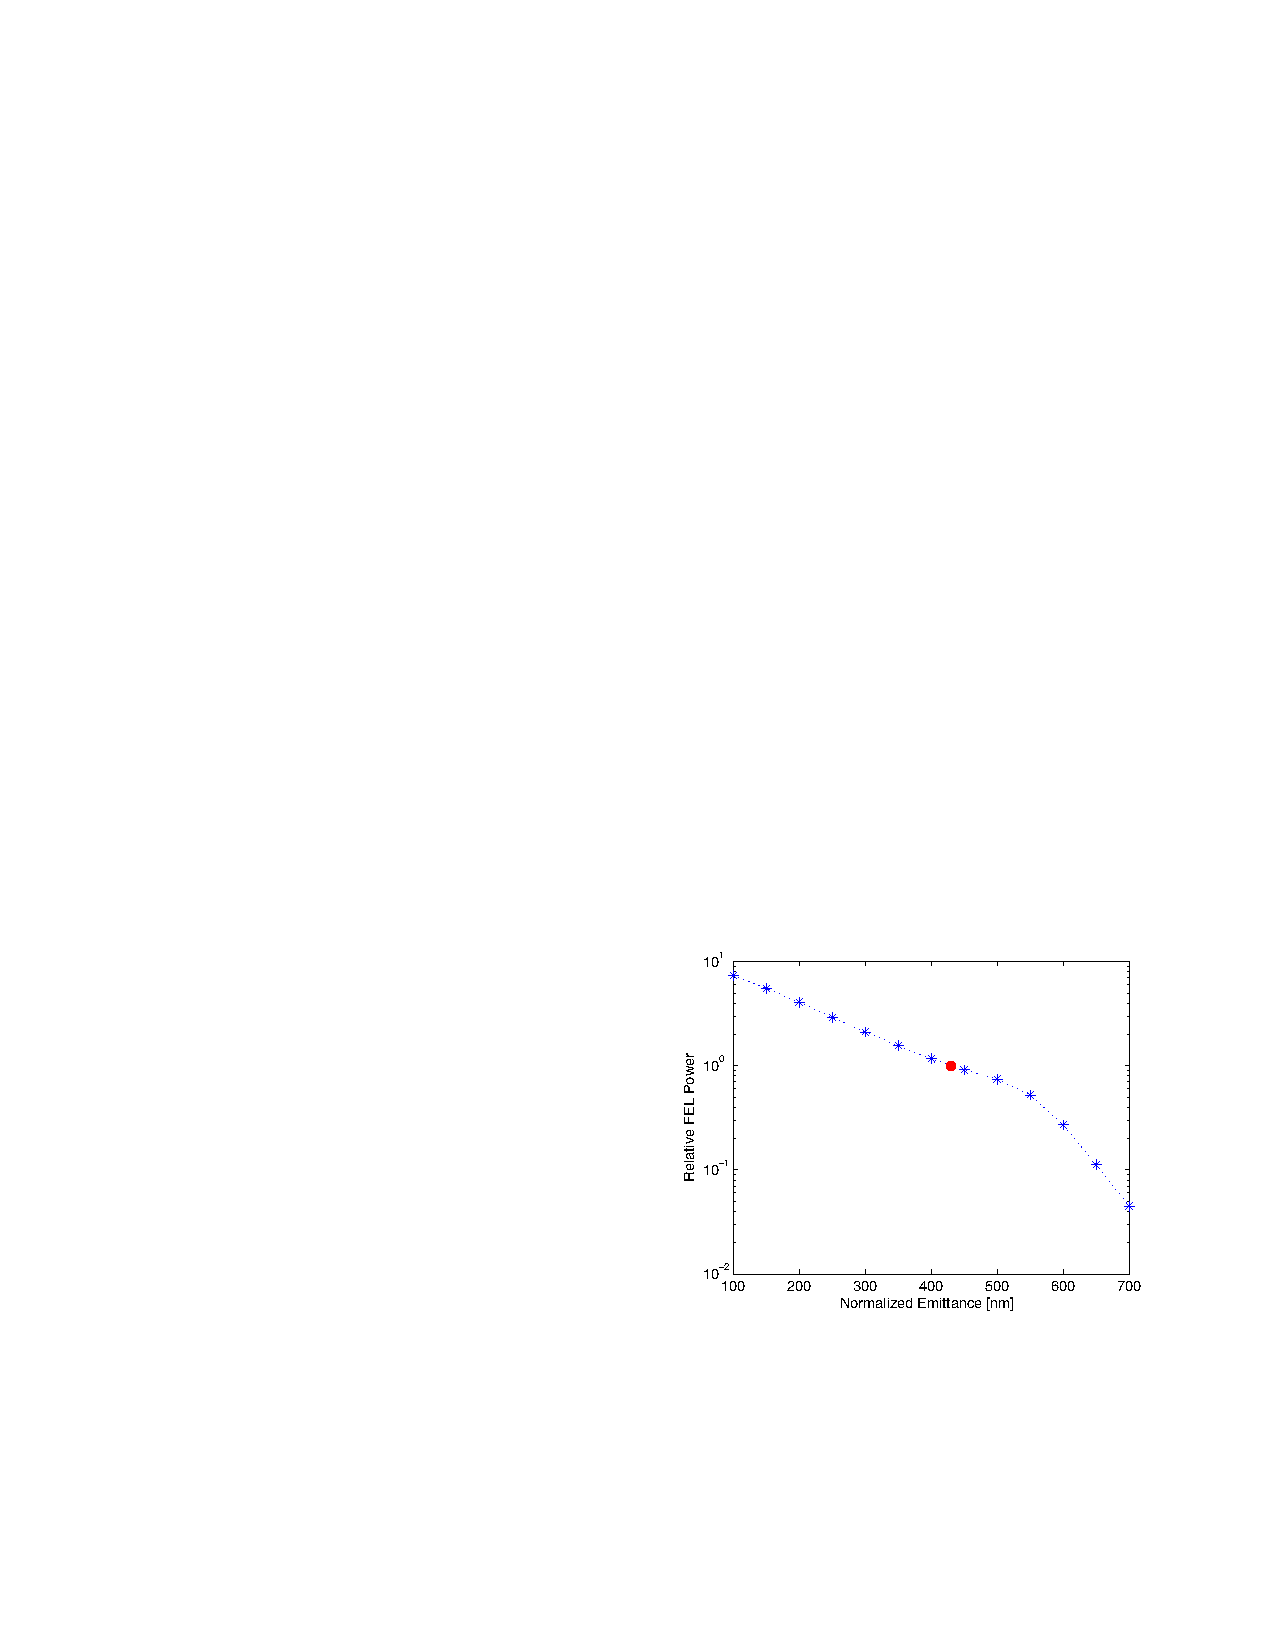
\includegraphics[width=0.6\textwidth]{xfel}
\caption{\label{fig:xfel} FEL 功率随发射度的变化\cite{prat2014emittance}。}
\end{figure}

\subsection{MeV UED}
MeV UED 即兆电子伏超快电子衍射,是一种将超短的 MeV 电子束作为探针,观测物质结构的快速变化过程实验手段。其原理见图 \ref{fig:ued}。
\begin{figure}[htbp]
\centering
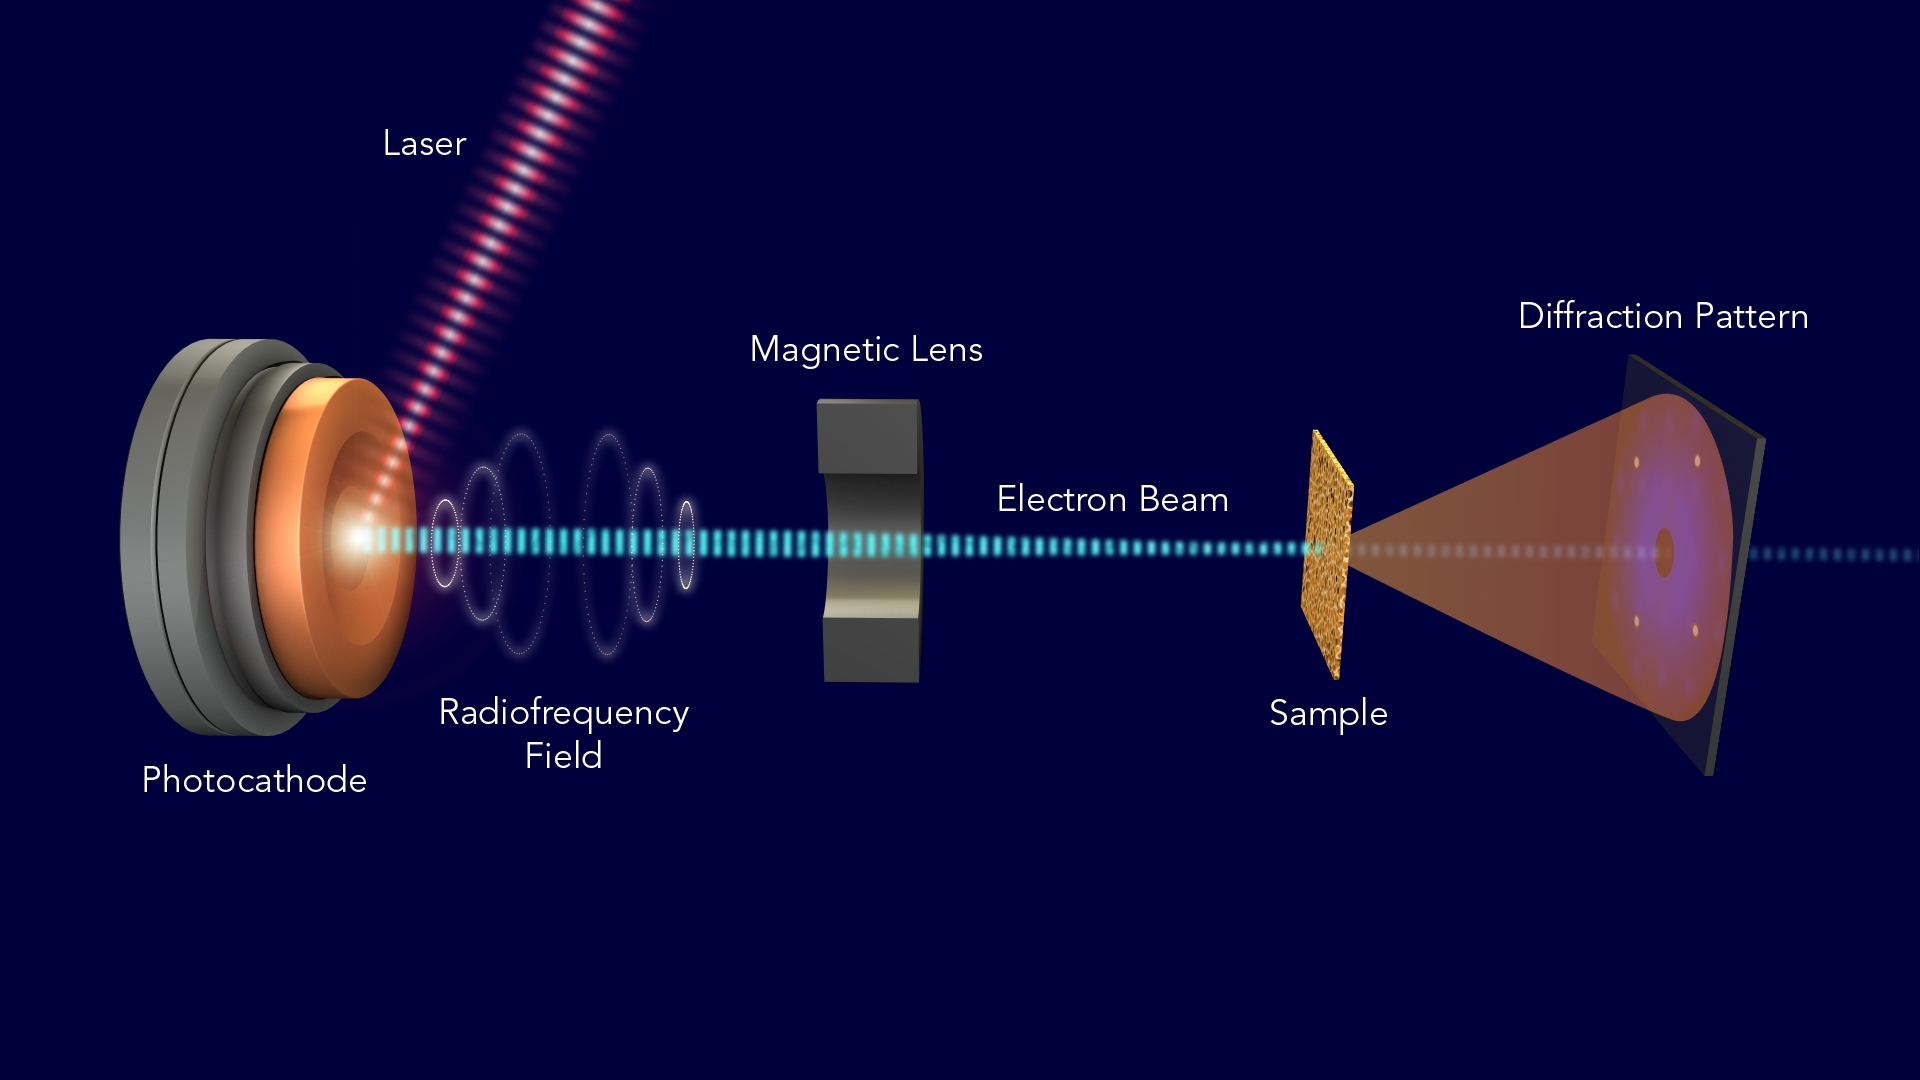
\includegraphics[width=0.8\textwidth]{ued}
\caption{\label{fig:ued} MeV UED 原理图\cite{Li:aa}。}
\end{figure}

MeV UED 的空间和时间分辨率如下式描述\cite{Weathersby:2015aa}:
\begin{eqnarray}
\Delta s &=& \frac{2\pi}{\lambda_e}\frac{\varepsilon_n}{\sigma_x}\\
\tau &=& \sqrt{\tau_e^2+\tau_{\text{ph}}^2+\tau_{\text{TOA}}^2+\tau_{\text{VM}}^2}
\end{eqnarray}
其中 $\lambda_e$ 为电子的康普顿波长。由上式可见在电子探针横向尺寸 $\sigma_x$(即样品上的电子束团 rms 尺寸)一定的情况下,空间分辨率随发射度 $\varepsilon_{n}$ 降低而减小,也即能分辨更细微的结构。同时电子的纵向尺寸越小,其时间分辨率也越小。一般 MeV UED 为保证足够的时间和空间分辨率,工作在低电荷量模式,电荷量 $Q < \SI{1}{pC}$,要求发射度 $\varepsilon_{n} < \SI{0.1}{mm\cdot mrad}$(达到 $<\SI{0.01}{mm\cdot mrad}$ 更好),束长尽量短($<\SI{1}{ps}$,若能达到 fs 量级更好)。根据发射度对电荷量的放缩关系($\varepsilon_n\propto\sqrt{Q}$),可知其发射度相当于 200\,pC 时 \emit{1.4}(达到更理想分辨率则需要 \emit{0.14}),其难度可见一斑。

\subsection{TSS}
汤姆逊散射源通过光子与相对论电子束对撞,产生高能 X 射线\cite{Milburn:1963aa,Fiocco:1963aa}。汤姆逊散射源的原理见示意图 \ref{fig:ttx}。
\begin{figure}[htbp]
\centering
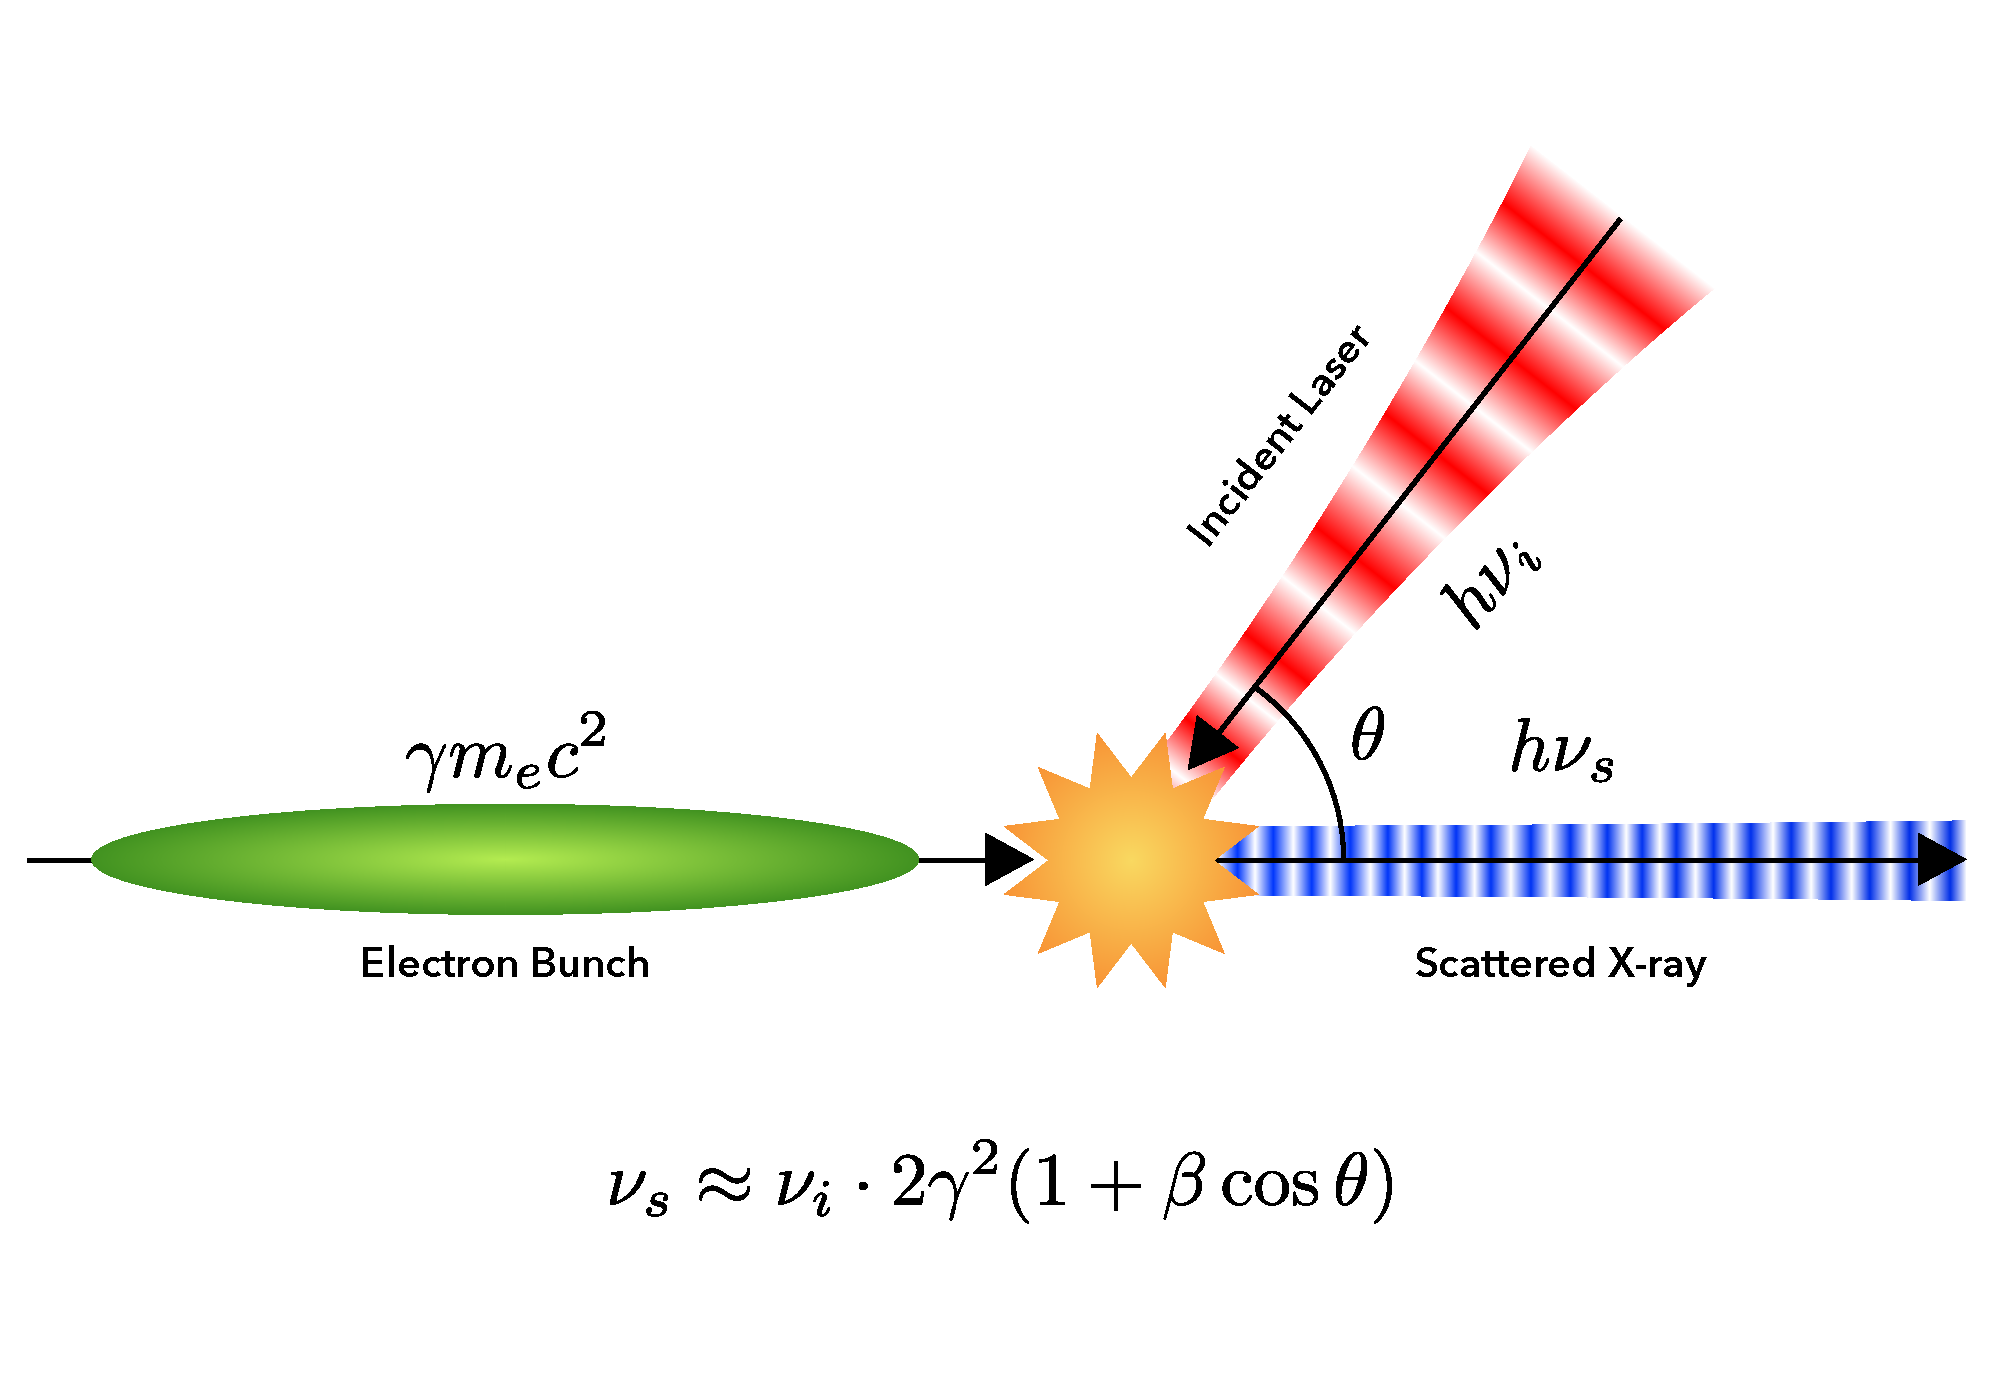
\includegraphics[width=0.6\textwidth]{ttx}
\caption{\label{fig:ttx} MeV UED 原理图。}
\end{figure}

激光与电子束正面对撞时,X 射线产额最大,此时 X 射线光子总数 $n_x$ 满足\cite{huangwenhui:2004aa}:
\begin{equation}
n_x = C_{\text{off}}\frac{n_en_l}{2\pi}\Sigma_{\text{th}}\frac{1}{\sqrt{(\sigma_{ex}^2+\sigma_{lx}^2)(\sigma_{ey}^2+\sigma_{ly}^2)}}
\end{equation}
其中 $n_e, \sigma_{ex}, \sigma_{ey}$ 是电子束的电子数目,x 向和 y 向尺寸;$n_l, \sigma_{lx}, \sigma_{ly}$ 是激光束的光子数目,x 向和 y 向尺寸。当电子束能散可忽略时,汤姆逊散射 X 射线源的亮度 $B_x$ 满足\cite{duyingchao:2006aa}:
\begin{equation}
B_x \propto \frac{n_x}{\varepsilon_{n, x}^2\varepsilon_{n, y}^2}
\end{equation}
从以上两式可知,电子束团发射度越小,X 射线光子总数越大,X 射线源亮度越高。对于清华大学加速器实验室的汤姆逊 X 射线散射源,目前实际运行在 0.5--0.7\,nC,发射度 \emit{1} 的参数下\cite{Qian:2012aa}。

\section{光阴极、光阴极微波电子枪与光阴极注入器}
为提供低发射度束流,常常采用光阴极注入器。光阴极注入器由光阴极微波电子枪、发射度补偿螺线管线圈和四极铁等束流操控元件及若干段加速管组成,其中光阴极微波电子枪是其核心。光阴极微波电子枪利用光电效应在光阴极表面产生电子束团,随后利用腔体内的高梯度射频场(几十至上百 MV/m),快速将束流加速到较高能量(几个到十几个 MeV),以抑制束团低能阶段空间电荷力对束流品质的破坏。

光阴极微波电子枪通过激光控制电子束团发射,可以实现阴极大电流密度发射及时间脉冲超短的电子束团,因此适用于产生亮度很高的电子束团。在光阴极注入器中,对电子束团进行进一步加速,并在加速过程中保持电子束的高亮度。

\section{基于光阴极注入器的低发射度束流研究现状}
如上节所述,激光入射到光阴极微波电子枪的光阴极上,通过光电效应激发光电子产生,光电子随后在电子枪中的高梯度射频场中加速,经过螺线管线圈、四极磁铁等束流操控元件以及加速结构进行进一步能量提升,最终抵达注入器出口。束流在光阴极表面产生时的发射度叫做热发射度,它决定了注入器出口处的束流发射度的最小值;然而,注入器出口束流发射度一般要大于热发射度,这是因为电子束在注入器的整个运动过程中,有很多因素都会造成发射度增长\cite{chao1980beam,Carlsten:1989aa,OShea:1996aa,OShea:1998aa,carlsten1995emittance}。追踪一个束流从产生到出射注入器的全部过程,就可更清晰地看到这些因素的影响。从光阴极表面出射时,由于阴极的粗糙度,可能造成热发射度的增长\cite{Bradley:1977aa};激光入射到粗糙表面时可能会激起表面等离激元\cite{Ritchie:1957aa},也会对发射度有一定影响。束团本身的线性及非线性空间电荷力也会造成投影发射度增长\cite{Kim:1989ab}。在电子枪的射频场运动时,线性和非线性 RF 效应都会造成投影发射度增长\cite{reiser1991free}。在螺线管线圈中,尽管投影发射度得到了补偿\cite{Carlsten:1989aa,Serafini:1997ab},但色散效应又会增大发射度\cite{yang2002experimental,Dowell:2010ab}。

自二十世纪八十年代起,经过二十多年的努力,人们已经逐步消除或补偿了其中的几个因素造成的发射度增长,下面简单回顾一下基于光阴极注入器的低发射度束流的发展。当然,除了追求低发射度,人们也追求高重频\cite{Petrarca:2010aa}或能工作于连续波(CW)模式的电子枪\cite{sannibale2012advanced,Filippetto:2013aa},但这并不是本论文的主题,故不在这里做综述。

\begin{figure}[htbp]
\centering
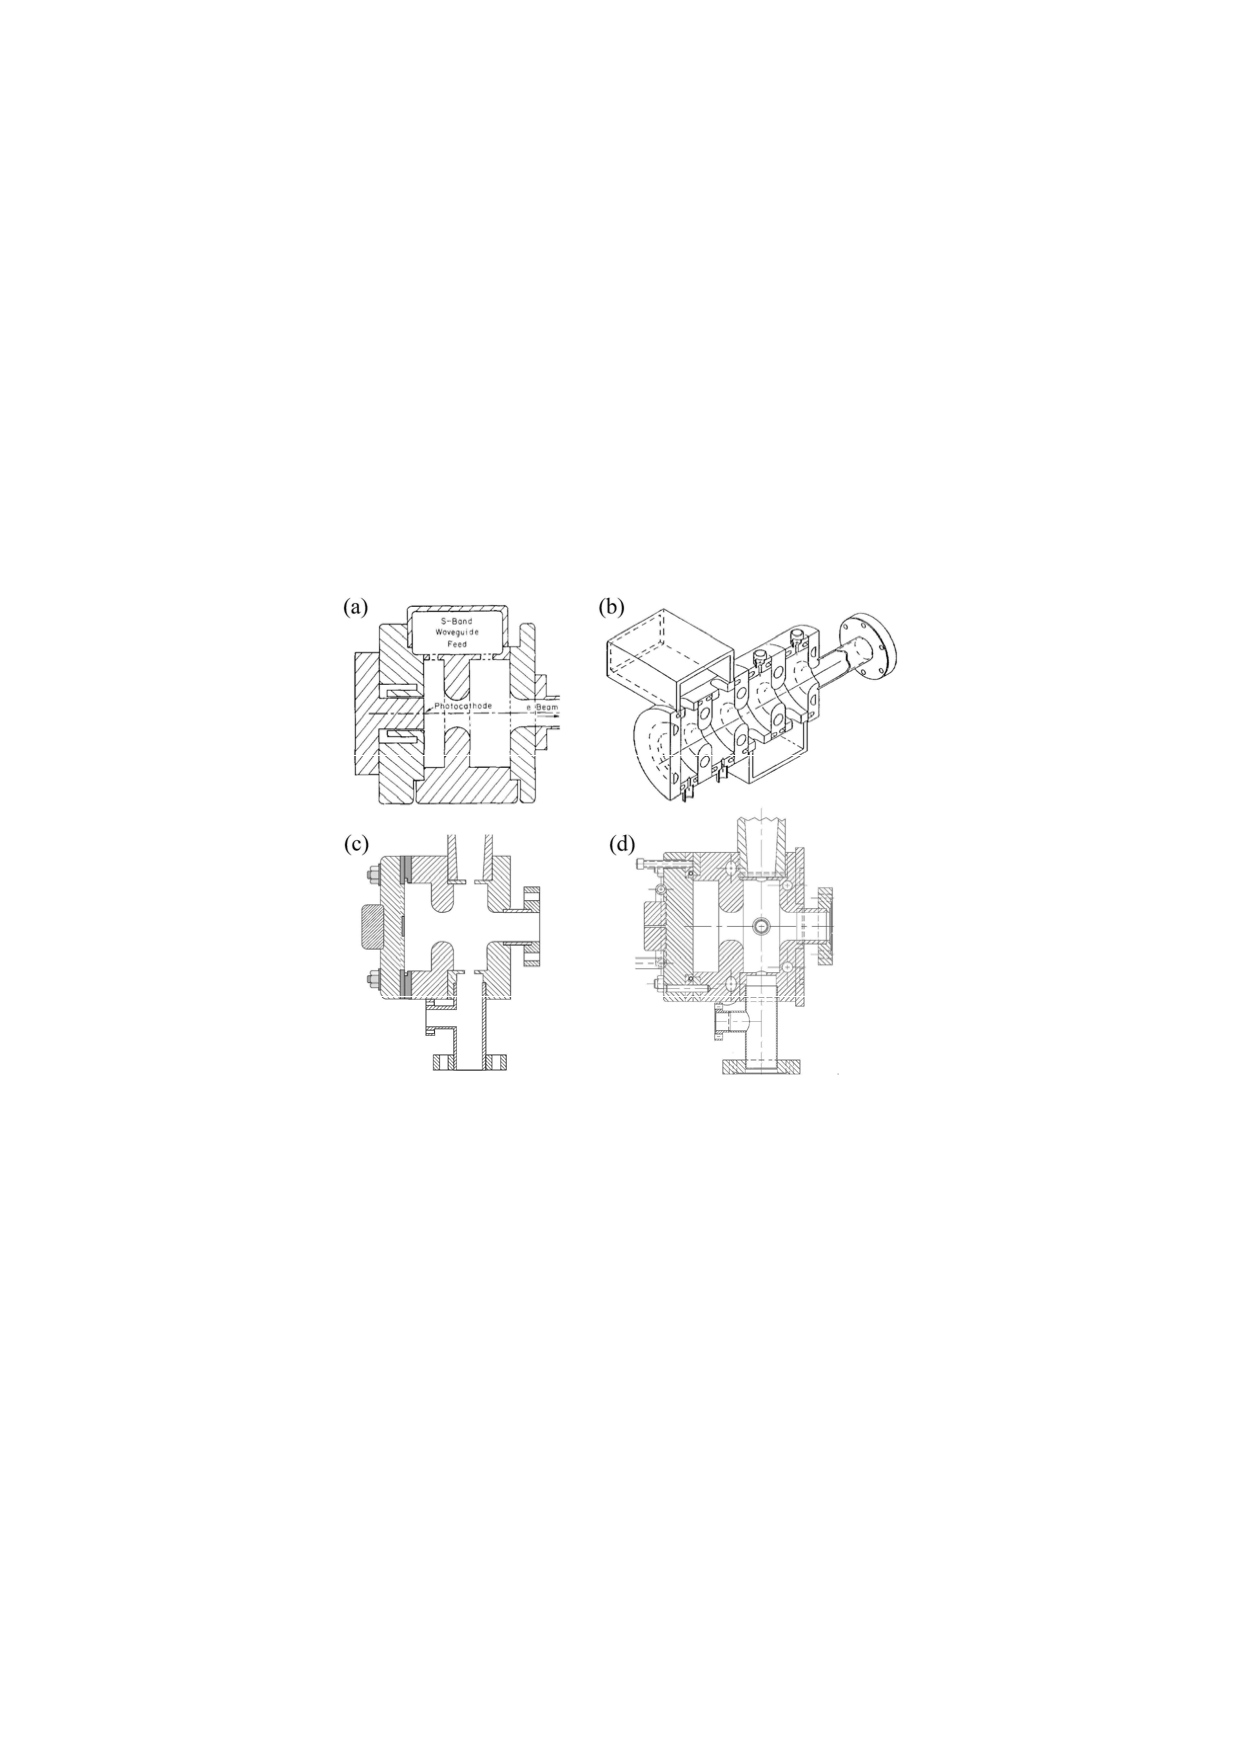
\includegraphics[width=0.7\textwidth]{guns}
\caption{\label{fig:guns} S 波段光阴极微波电子枪结构示意图\cite{Qian:2012aa}。}
\end{figure}

第一阶段在 1985 年光阴极微波电子枪注入器搭建成功\cite{Fraser:1986aa,Fraser:1987aa}后开始。该阶段光阴极注入器出口处发射度主要由电子枪本身限制,因此优化主要集中在抑制电子枪中线性/非线性 RF 场及空间电荷力造成的切片和投影发射度增长。McDonald 给出了电子枪理想边界,使横向 RF 场为线性\cite{McDonald:1988aa};Kim 解析了光阴极微波电子枪中束流的运动,并提出通过减小束团纵横比来抑制空间电荷力发射度增长,以及减小束团长度来抑制纵向非线性 RF 发射度增长\cite{Kim:1989ab};为进一步抑制非线性空间电荷力,增大阴极表面场强从而有首腔 0.5 cell 的设计\cite{McDonald:1988aa};同时为补偿关联投影发射度提出在电子枪上应用螺线管线圈\cite{Carlsten:1989aa}。

第二阶段则在上一阶段基础上,进一步优化电子枪结构,以消除多极场/干扰模式对发射度的影响,进一步提高束团亮度。为达到对束团更强聚焦以及束长压缩以提高束团亮度,首腔从 0.5 cell 变到 0.6 cell\cite{Lehrman:1992aa};由于关联发射度增长被抑制,电子枪中多极场对发射度的改变显现出来,因此电子枪结构/功率馈入变得对称化\cite{Palmer:1998aa,guan2007study},并采用跑道型耦合孔抑制多极模\cite{Limborg:2005vn, Akre:2008aa};$\pi$ 模工作时激发起的 0 模对发射度造成影响,因此优化束流孔以扩大频率间隔\cite{Palmer:1998aa}。电子枪腔型的发展过程见图 \ref{fig:guns}。在这一阶段中,一个重要的里程碑是应用于 LCLS 的光阴极注入器中的光阴极微波电子枪,它驱动了世界首台硬 X 射线自由电子激光(即直线加速器相干光源 LCLS),它集成了这一阶段对电子枪腔型的优化,其腔型设计见图 \ref{fig:lcls-gun}。

\begin{figure}[htbp]
\centering
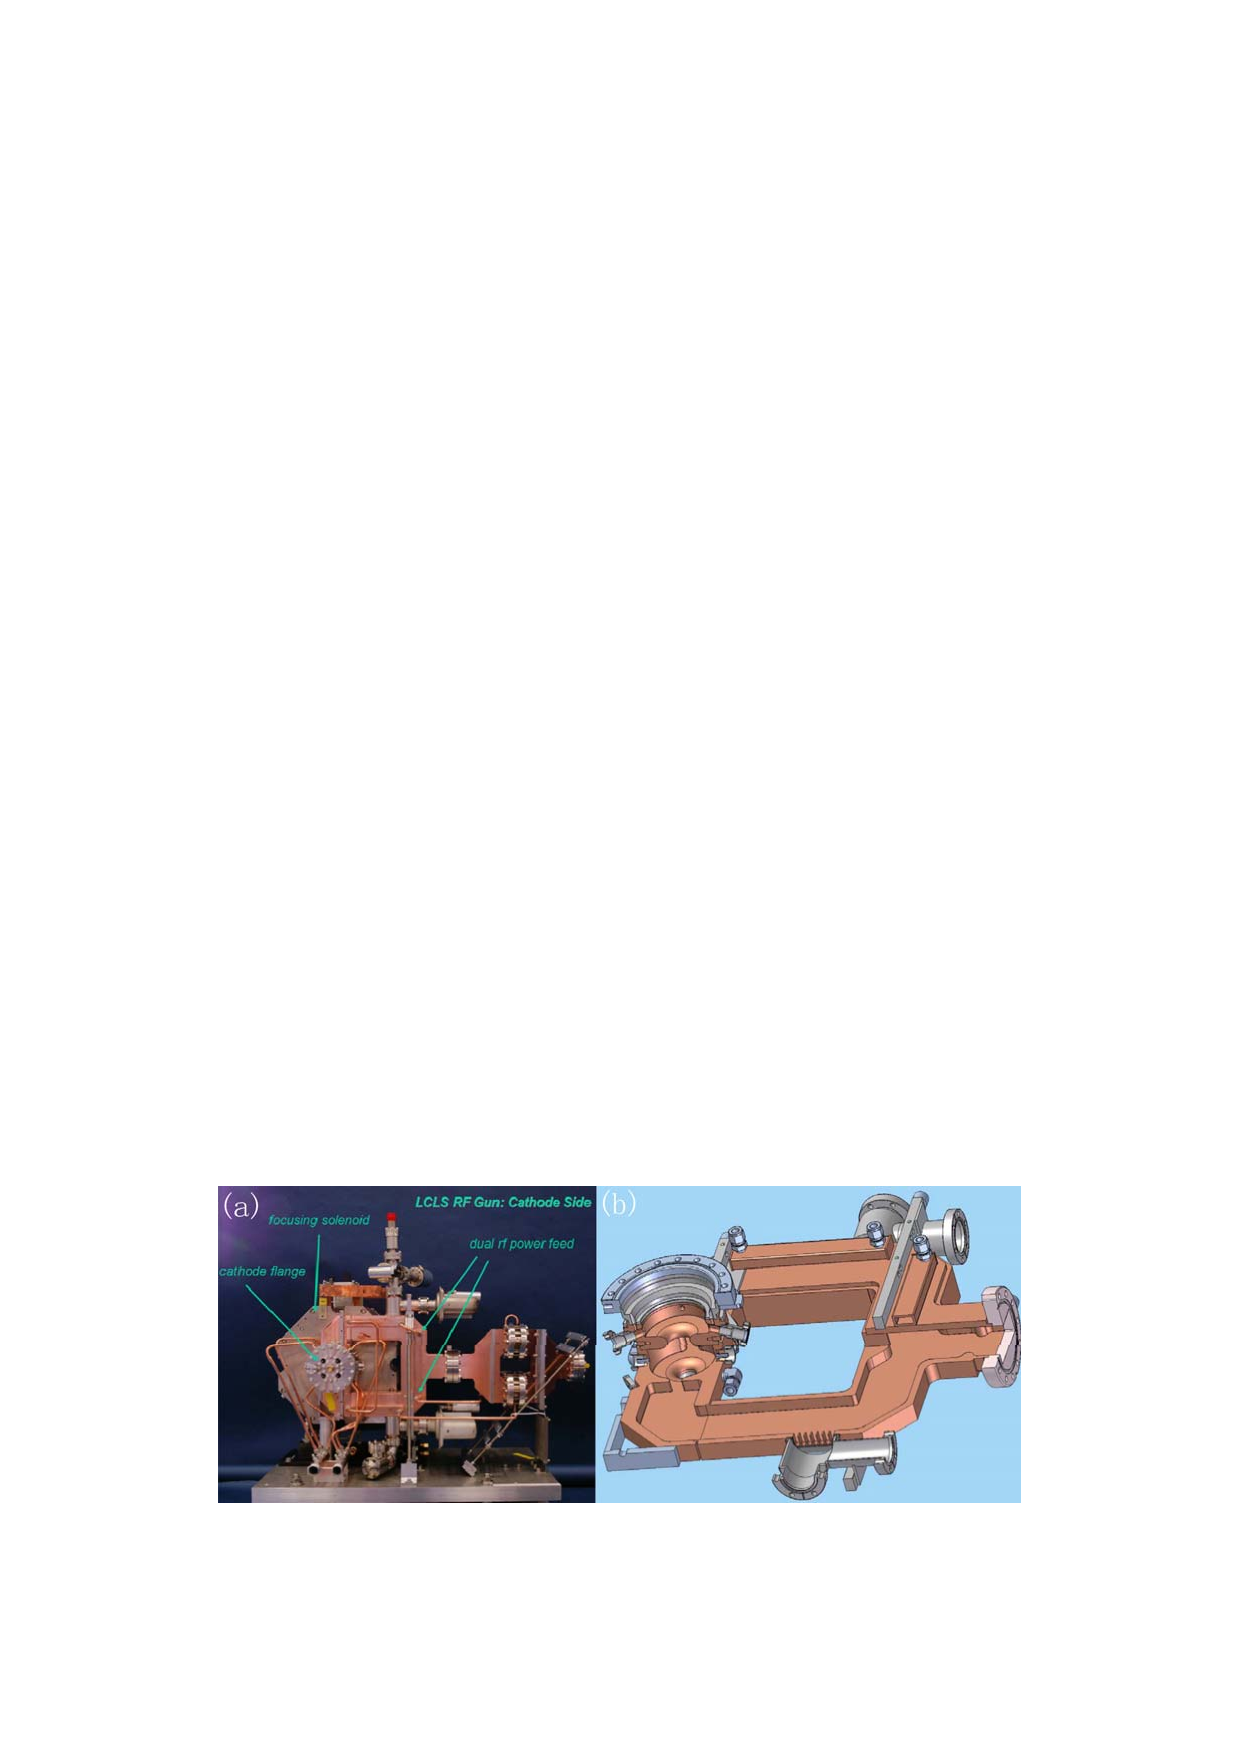
\includegraphics[width=0.7\textwidth]{lclsgun}
\caption{\label{fig:lcls-gun} LCLS 光阴极微波电子枪\cite{Qian:2012aa}。(a)电子枪实物图;(b)电子枪剖面图。}
\end{figure}

第三阶段中,电子枪的腔型造成的发射度增长已经很小,注入器出口处的发射度近似由热发射度、非线性 RF 发射度及非线性空间电荷发射度组成\cite{Qiu:1996aa}。此阶段人们开始优化整个注入器结构及激光参数。针对非线性空间电荷力,KV 分布\cite{Kapchinskij:1959aa}被动力学模拟证明可以有效抑制非线性空间电荷力发射度增长\cite{Limborg-Deprey:2006aa,Khojoyan:2013aa},进而激光整形、扁平束发射(pancake regime)\cite{bazarov2009maximum}及笔形束发射(cigar regime)\cite{filippetto2014maximum}等可以产生 KV 分布束团的方法被提出及模拟或实验验证\cite{Khojoyan:2013aa,Khojoyan:2014aa,Musumeci:2008ab,Li:2012aa}。对于非线性 RF 作用,Dowell 和 Raguin 分别提出了两种空间叠合型双频电子枪\cite{Dowell:2004aa,Raguin:2005aa}以实现纵向线性 RF 场,消除非线性 RF 发射度增长。

第四阶段,也即当前阶段中,注入器出口处的发射度已迫近热发射度\cite{li2012multi,gulliford2013demonstration,karkare2011effect,karkare2015effects},此时阴极的地位变得重要:阴极材料的选取\cite{Cultrera:2014ab},阴极表面形态(表面粗糙度,污染)\cite{Vecchione:2012aa,Vecchione:2013aa,Ling:2013aa},以及阴极表面上的物理过程:肖特基效应,空间电荷限等都会对注入器出口处发射度产生较大影响\cite{qian2012experimental}。在这个阶段中,人们提出了光阴极表面极限亮度并进行了实验验证\cite{bazarov2009maximum,filippetto2014maximum}。

综合以上,对注入器出口束流品质的优化基本分为两个部分,即对光阴极表面热发射度的优化,以及对注入器多个参数的优化,以将光阴极的横向亮度保持到注入器出口。下面详细介绍这两部分的相关研究和进展。

\subsection{光阴极热发射度的优化}
\subsubsection{改变材料及激光波长}
对于光阴极上的热发射度,Dowell 采用三步模型给出了金属光阴极体发射的发射度\cite{Dowell:2006aa,dowell2009quantum}:
\[
	\varepsilon_{n} =\sigma\sqrt{\dfrac{\hbar\omega-\phi_{\mathrm{eff}}}{3mc^2}}
\]
该公式揭示了体发射情形热发射度与金属材料及激光波长的关系。该公式催生了一系列调变金属材料与激光波长来优化热发射度的研究,如 PSI 对四种不同金属阴极热发射度及量子效率的实验\cite{hauri2010intrinsic},实验中使用了可微调中心波长的激光,通过对每种金属扫描激光波长,同步测量发射度与 QE 变化来验证理论公式。实验中测量了四种金属阴极:Cu,Mo,Nb,Al。实验直接验证了可以通过减小光子能量与有效逸出功的差距来降低热发射度,也同时验证了热发射度降低时,其对应的 QE 也会降低。该实验的结论是在引出场强较低(25 MV/m)时,由于能够同时提供可接受的 QE 以及最小的热发射度,Cu 是最适合用来做光阴极的金属。当入射激光波长为 282 nm,引出场强为 25 MV/m  时,Cu 的归一化热发射度为 0.41\,mm$\cdot$mrad/mm,QE 为 $5\times10^{-6}$\cite{hauri2010intrinsic}。

\subsubsection{采用新的发射机制}
人们提出了光场使能的场致发射(Photo Field Emission,PFE)来从原理上降低热发射度\cite{Reifenberger:1979aa}。光场使能场致发射本质上是一种场致发射,场致发射是利用量子隧穿效应的电子发射机制,其好处在于出射电子横向动量极小,因此可以有很低发射度,缺点是依靠高梯度微波场发射时其发射束团长度较长(ns 量级)且电荷量较小。若用激光作用于场致发射阴极(一般是针尖或针尖阵列)上,可以提高电子能量,使隧穿概率升高,原来不能场致发射的场强下也可进行场致发射。PFE 结合了场致发射发射度低和光电发射可控以及可产生超短束团的优点。PFE 提出后,针对 XFEL 上的应用陆续有实验\cite{Ganter:2008aa,Mingels:2012aa,Mingels:2013aa,Mingels:2014aa}及模拟研究\cite{Fallahi:2014aa}开展。如采用单 ZrC 针尖(半径 5\,$\mu$m)阴极,阴阳极之间加 60\,kV,2\,ns,30\,Hz 的脉冲高压,使用 16\,ps,266\,nm 的短束长激光入射就可以获得高 QE(针尖附近场强高)的同时实现低发射度。PFE 发射理论上可以在引出电荷 150\,pC 时获得 \emit{0.05} 的发射度\cite{Mingels:2014aa}。

\subsubsection{抑制阴极表面效应}
金属阴极表面一般有表面污染及表面粗糙起伏,这也会造成发射度的变化。表面污染一般是阴极加工时引入,例如电抛光时引入的 S、C、O 等元素。实验研究证明不同污染主要影响金属表面逸出功\cite{Chelvayohan:1982aa,Opower:2006aa,Valizadeh:2013aa}。例如对于银阴极,表面的硫污染会导致逸出功升高,表面的碳污染却会导致逸出功降低\cite{Chelvayohan:1982aa}。应对阴极表面污染造成的影响,目前较常见的解决方法是激光清洗\cite{Brachmann:2011aa}以及 Ar 原子轰击清洁阴极表面\cite{Chelvayohan:1982aa,Valizadeh:2013aa}。实验证明,利用 Ar 原子清洁可使阴极表面的 C 和 O 含量大幅降低,对量子效率的提升有很大帮助\cite{Valizadeh:2013aa};利用激光清洗,减小激光功率,缩短激光扫描步长,也会对量子效率有显著提升\cite{Brachmann:2011aa}。

另外对于光阴极微波电子枪中常用的多晶铜(晶面可能为(100),(110) 和 (111))阴极,研究发现阴极表面晶面不同的位置其逸出功也不同,且可能有高达 400\,meV 的差别\cite{Renault:2006aa},这也会引起热发射度的增长。可能的解决方案是采用单晶铜阴极,受限于单晶金属的造价,一般采用 cathode-plug 的方式进行应用\cite{Ganter:2013aa}。

对于阴极表面粗糙度造成的热发射度增长的研究,一般采用二维正弦表面模型进行研究\cite{He:2004aa,Krasilnikov:2006aa,Karkare:2011aa}。阴极表面粗糙度热发射度增长主要来自两方面:即表面离散效应(slope effect)和横向电场效应(field effect)\cite{Bradley:1977aa}。阴极的粗糙度被认为是造成热发射度实验测量值与理论值差异的主要原因\cite{qian2012experimental,Vecchione:2012aa,schubert2013bi}。尽管有基于二维正弦表面的定性粗糙度热发射度公式对两种增长效应给出物理上的解释,但是由于缺乏针对一般粗糙阴极表面的粗糙度热发射度公式(slope effect 主要是数学上的困难,field effect 主要是物理上的困难),粗糙度热发射度公式中的参数主要靠实验拟合,其说服力有限,且目前无法给出想抑制粗糙度热发射度到一个水平以下,对表面加工的要求具体是多少。

阴极表面粗糙度在合适激光波长的作用下有可能激励起表面等离激元\cite{Novotny:2012aa}。表面等离激元的产生对光阴极亮度既有好处又有坏处:表面等离激元可以将光子囚禁在金属阴极表面,这会增大阴极对激光的吸收率,同时表面等离激元会极大加强阴极上的激光功率密度,进而提高 QE;但另一方面,表面等离激元所要求的粗糙阴极表面形态会造成发射度的增长,这会降低阴极亮度。利用表面等离激元性质的阴极有两类:衰减全反射阴极(ATR)和纳米表面阴极(NPC)。其中衰减全反射阴极利用棱镜在金属薄膜表面激发表面等离激元,既有高 QE 的优点又兼具平面阴极低发射度的优点,但其问题在于由于微波的趋肤深度一般大于金属薄膜厚度,会造成场泄漏,难以集成在光阴极微波电子枪中\cite{Watanabe:2011aa,Neo:2012aa};而 NPC 阴极经实验验证,当工作在多光子光电发射模式\cite{Musumeci:2010aa},其电子产额有上百倍的增长,且归一化热发射度相对于平整阴极只增长不到 1 倍\cite{Polyakov:2013ab,Li:2013ac},因此是有潜力产生高亮度束团的候选。目前对于 NPC 阴极的研究仅限于铜阴极(材料易获得易加工),其他材料的发射特性有待研究。

\subsection{光阴极注入器中发射度的保持}
热发射度的优化和光阴极注入器的优化是密不可分的:即使在阴极表面产生了超低热发射度,因其可能存在的非线性空间电荷力和非线性 RF 场作用,也极有可能无法将超低热发射度保持到光阴极出口。因此进行光阴极注入器优化时,需要同时考虑阴极上的激光参数。下面介绍光阴极注入器优化的重要进展和工作。

\subsubsection{最高场强的优化}
文献\cite{wang1997field}指出加速结构中的射频击穿(RF breakdown)场强与频率的二分之一次方成正比,因此提高电子枪及加速管的工作频率可以提高腔内最大场强,进而更有效地抑制束流发射阶段空间电荷力发射度增长。目前绝大多数注入器均采用 S 波段或 L 波段(LCLS 采用 S 波段注入器\cite{Zhou:2015aa},PSI 目前也采用 S 波段注入器\cite{prat2014emittance},Cornell 注入器束线中采用 L 波段超导加速腔\cite{shemelin2012frequency,Bartnik:2015aa},DESY 的 PITZ 注入器中采用 L 波段电子枪\cite{Krasilnikov:2012aa})Limborg 于 2011 年搭建了 X 波段光阴极注入器测量平台\cite{Limborg-Deprey:2011aa},第一台 X 波段光阴极注入器于 2016 年成功搭建\cite{Limborg-Deprey:2016aa},其中阴极发射场强高达 150\,MV/m,其 100\,pC 对应发射度为 \emit{0.7},虽然发射度较大但其纵向 rms 束长极短,只有 400\,fs,亮度很高。另外一个提高注入器最高场强的办法是降低阴极温度。研究发现,当电子枪运行于低温($\sim$ 20\,K)时,其表面所允许的最大场强大幅上升\cite{Rosenzweig:2016aa},可以利用这个性质来减小激光横向尺寸从而降低热发射度,以及进一步抑制束团发射阶段的非线性空间电荷效应造成的发射度增长。

\subsubsection{激光参数的优化}
KV 分布\cite{Kapchinskij:1959aa}可以有效抑制非线性空间电荷力发射度增长\cite{Limborg-Deprey:2006aa,Khojoyan:2013aa},相对于常用的柱形均匀分布束团,三维均匀椭球束团的注入器出口处发射度可降低 30\%\cite{Khojoyan:2014aa}。产生 KV 分布的束团目前常用的有三种方法:激光整形、扁平束发射(pancake regime)及笔形束发射(cigar regime),其对发射度增长的抑制效果已被实验初步验证\cite{Khojoyan:2013aa,Khojoyan:2014aa,Musumeci:2008ab,Li:2012aa}。目前激光整形技术精度不够,离三维均匀椭球尚有一定偏差,这会造成不小的发射度增长\cite{Khojoyan:2013aa};扁平束在发射过程中,由于其极强的纵向空间电荷力,扁平束流会在很短时间内纵向膨胀成为一个准 KV 分布束团,但由于阴极表面的镜像电荷效应,初始服从 KV 分布的束团若电荷量太大会出现畸变,因此只限于产生低流强的束团\cite{Musumeci:2008ab};笔形束与扁平束正相反,靠其极强的横向空间电荷力,在发射后迅速横向膨胀成为一个准 KV 分布束团,且由于其横向尺寸很小,可产生 nm 级发射度\cite{Li:2012aa}。最近的遗传算法优化发现,将阴极上的初始束长拉长,有助于保持阴极热发射度,在注入器出口处可获得更低发射度的束流\cite{Qian:2016aa}。

\subsubsection{自动优化算法}
由于光阴极优化的多输入变量多优化目标的本质(优化发射度时要同时兼顾峰值流强),多目标进化算法最早于 2005 年被 Bazarov 应用于光阴极注入器优化\cite{Bazarov:2005aa}。在该工作中,Bazarov 将 NSGA-II 遗传算法\cite{Deb:2002aa} 应用于 Cornell 的直流高压枪注入器优化,遗传算法优化器对于 100\,pC 情形给出了 \emit{0.1} 的结果,对于 1\,nC 情形给出了 \emit{0.7} 的结果,从而证明了遗传算法优化器的可靠性与相对于人工的优势,即可能获得全局最优解。Qiang 将差异进化算法(differential evolution algorithm)应用于类 LCLS 的注入器优化,由于算法的贪婪(greedy)\cite{cormen2009introduction}本质,大大缩短了遗传算法优化所需要的时间\cite{Qiang:2013aa},当然与此同时带来的问题是可能无法获得全局最优解。Bettoni 受遗传算法启发,将分段单纯形法应用于 SwissFEL 注入器束线优化中,并获得 10\,pC 电荷量下 \emit{0.08} 以及 200\,pC 电荷量下 \emit{0.14} 的优化结果\cite{Bettoni:2015aa}。

\subsection{超低束流发射度的测量}
优化获得注入器出口处的超低发射度束流后,还需进行实验测量已验证优化效果,下面介绍低发射度束流的常用发射度测量方法。根据束流发射度的统计定义,束流发射度由横向束斑尺寸与横向动量参数共同决定。实验中,电子束的横向束斑尺寸信息可通过荧光屏上的束流图像直接测得~\cite{Graves:1997aa,Walasek-Hohne:2011aa},因此,发射度的测量问题主要集中在对束流的横向动量信息的获取~\cite{lee2015review}。

为叙述方便起见,引入平均横向动能(Mean Transverse Energy,MTE)的概念\cite{bazarov2008thermal,bazarov2009maximum,lee2015review}:
\begin{equation}
\text{MTE} = \frac{1}{2}m\langle v_\perp^2\rangle
\end{equation}
其中 $m$是电子质量,$v_\perp$为电子的横向速度。MTE与光阴极束流归一化热发射度 $\Delta_{x}$ 关系如下:
\begin{equation}
\label{eq:es_MTE}
\Delta_{x} = \sqrt{\frac{\text{MTE}}{mc^2}}
\end{equation}

目前,已有多项研究对MTE的数值进行理论推导~\cite{karkare2011effect,karkare2013monte}与实验测量~\cite{bazarov2009maximum,engelen2014effective,dowell2009quantum,qian2012experimental}。但是对于超低发射度的测量依然处以探索研究阶段,下面主要介绍针对 $\text{MTE}<\SI{100}{meV}$(等效归一化热发射度 $<$ 0.4\,mm$\cdot$mrad/mm)的发射度测量~\cite{hauri2010intrinsic,lee2015review}。

\begin{table}[htbp]
\caption{常用的发射度测量方法}
\label{tab:method}
\centering
\begin{tabular}{p{2cm}p{3.5cm}p{5cm}p{2.5cm}}
\toprule
方法 & 测量设置 & 方法的不足 & MTE测量值 \\
\midrule
半球形分析仪~\cite{Palczewski:2010aa} & 施加不同的电压来区分测量不同能量、不同空间分布的发射电子 &1)对功函数敏感;2)非直接的测量;3)易被系统中的杂散电磁场干扰;4)当发射电子动能小于1\,eV时测量结果不可靠;5)不适用于强场(MV/m)电子枪环境 & $\sim$ 100\,meV~\cite{Droubay:2014aa} \\
渡越时间分析器~\cite{Wang:2012aa,Sertore:2004aa}  & 利用延迟线探测器测量发射电子的渡越时间和横向位置 &1)需要一个亚皮秒的激光;2)易被环境中的电磁场干扰;3)当发射电子动能小于1\,eV时测量结果不可靠;4)不适用于强场(MV/m)电子枪环境 & $\sim$130$\pm$5\,meV~\cite{sertore2004cesium} \\
能量分析谱仪~\cite{Karkare:2015aa,Orlov:2001aa} & 测量发射电子在纵向磁场下的运动 & 1)不适用于强场(MV/m)电子枪环境;2)纵向磁场也许会影响光电发射的过程,测量结果不准 & $\sim$25$\pm$2.5\,meV~\cite{Orlov:2001aa} \\
最小束斑扫描法~\cite{engelen2014effective,bazarov2008thermal,bazarov2011thermal,anderson2002space,hauri2010intrinsic} & 电子枪加聚焦元件组 & 需要准确的磁场标定测量 &  $\sim$1\,meV~\cite{engelen2014effective}\\
束流采样或胡椒瓶法~\cite{anderson2002space,Reiser:2008aa,gulliford2013demonstration} & 两片光栅加探测器或者一片光栅加探测器 & 对于低MTE的束流,分辨率与束流初始发射度相当 & 35\,meV ~\cite{Maxson:2015aa}\\
自由膨胀法~\cite{feng2015novel} & 加速结构和自由漂移段 & 1)存在激光衍射效应;2)需要极小的激光光斑;3)使用的网格不均匀 & 27\,meV~\cite{feng2015novel} \\
横向能散谱仪~\cite{jones2013commissioning}  & 在加速段中自由膨胀 & 1)需要极小的激光光斑; 2)无法应用在kV/m的环境中 & $\sim$45$\pm$7\,meV~\cite{jones2013commissioning} \\
\bottomrule
\end{tabular}
\end{table}

对于目前有的发射度测量方式,其总结与对比可参见表格 \ref{tab:method}\cite{lee2015review}。其中典型的几个方法简介如下:

(1)半球形分析器\cite{Palczewski:2010aa}和渡越时间探测器\cite{Wang:2012aa, Sertore:2004aa}常用于角分辨的光电子能谱(Angle Resolved Photoemission Spectroscopy,ARPES)测量实验中~\cite{Palczewski:2010aa,Zhang:2011aa}。采用能量大于材料逸出功的光子照射在材料表面,利用半球形分析器或者渡越时间探测器测量发射电子的能量、对应的方位、极化角分布等参数,通过对测量材料的旋转,可以获得全角度范围的光电子信息,从而统计给出MTE参数。由于低能的发射电子(<1\,eV)易受系统中杂散电磁场的干扰,该系统适用于发射电子能量在几个eV能量范围~\cite{Droubay:2014aa,Sertore:2004aa}。

(2)最小束斑扫描法常用于加速器光阴极注入器的在线发射度测量~\cite{engelen2014effective,bazarov2008thermal,bazarov2011thermal,anderson2002space,hauri2010intrinsic},根据聚焦元件的种类,也称为螺线管扫描法或者四极磁铁扫描法。其装置设置的简单示意图如图~\ref{fig:waist_scan}(a)所示,电子经过电场的加速后,进入漂移段,通过改变磁透镜(螺线管或四极磁铁)的电流,改变其对束流的聚焦焦距,从而改变束流的包络。采用荧光屏和相机观测记录一定距离之后的束斑尺寸,束斑尺寸大小随着透镜强度的变化如图~\ref{fig:waist_scan}(b)中所示的曲线。根据束流传输理论,当所有传输元件(加速段、聚焦元件等)为线性元件,线性传输矩阵记为$\bf{\text{R}}=\bf{\text{R}}_{i\to f}$,描述束流从位置$i$到位置$f$的束斑联系矩阵,即~\cite{bazarov2008thermal}:
\begin{equation}
\label{eq:waist_scan}
\left(\sigma_x \sigma_{\theta_x}\right)_f = R\left(\sigma_x \sigma_{\theta_x}\right)_i
\end{equation}
其中,束流参数包含了rms束斑尺寸$\sigma_x$和rms束流发散角$\sigma_{\theta_x}$。由于$\bf{\text{R}}$已知,多组测量拟合下,可反推获得束流初始,即光阴极出口处的发射度(或者MTE)的信息。该方案需要对传输矩阵以及荧光屏上的束斑尺寸进行准确测量,传输元件的非线性效应、非线性空间电荷力效应等会引起测量误差、同时,该方案对于超低发射度的测量需要提高相机、荧光屏对束斑尺寸的分辨率。
\begin{figure}[htbp]
\centering
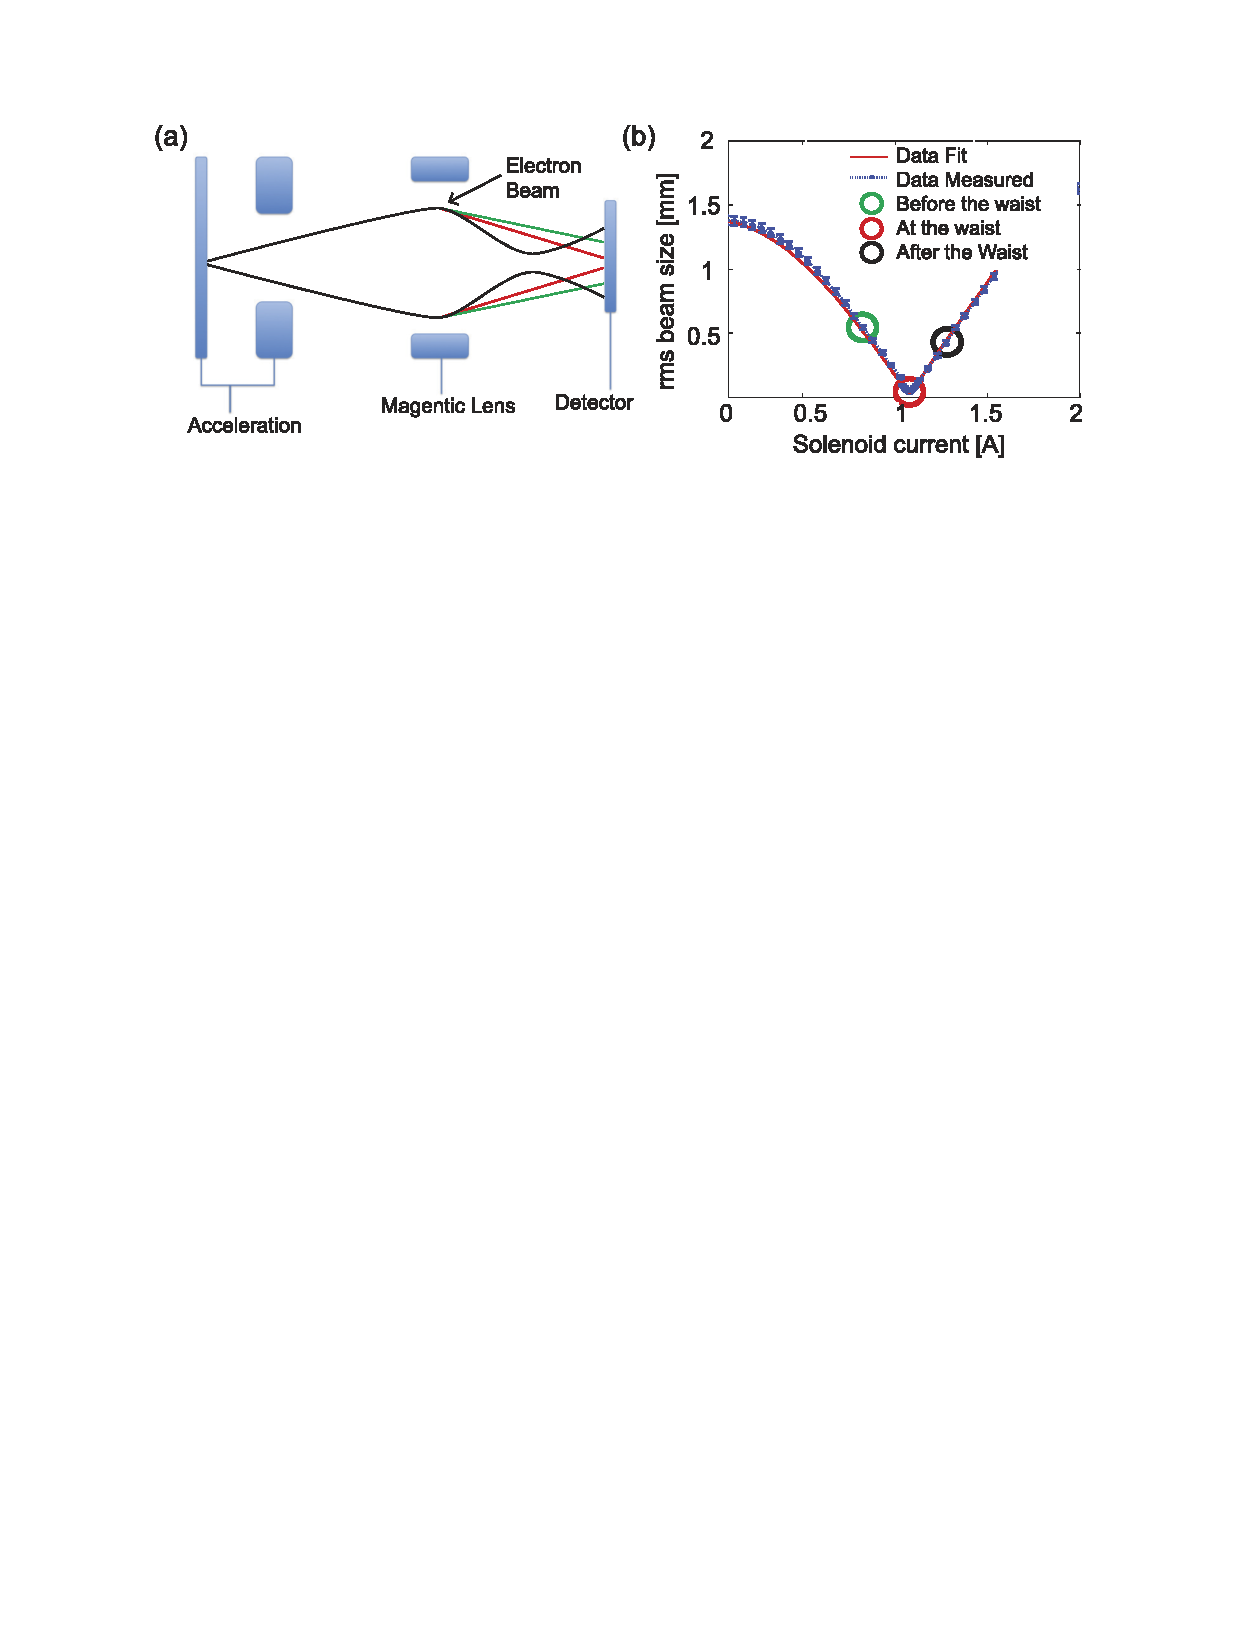
\includegraphics[width=0.9\textwidth]{waist_scan}
\caption{\label{fig:waist_scan} 最小束斑扫描法原理示意图}
\end{figure}

(3)束流采样或者胡椒瓶盖法\cite{anderson2002space,gulliford2013demonstration,li2012nanometer}:这类方法的主要优点是可以扫描获取整个束流的横向相空间。在两个窄缝系统的束流采样方案中,两个带有窄缝金属平板相隔一定距离,放置于束流前进方向,由于平板足够厚,只有窄缝位置处的束流可以通过。第一个窄缝选择出距离束斑中心一定位置的一定范围内的部分电子,被选择出来的电子进一步漂移,通过第二个窄缝的筛选,只有几个电子被最终的探测器(如测量电荷量的法拉第桶)收集,通过扫描窄缝的位置,该方法可以获取整个束流的横向分布与横向散角分布,从而获得束流的横向相空间。胡椒瓶法是对上述方案的改良,用胡椒瓶盖形状的栅网对束流进行采样,采用偏转腔替代法拉第筒对筛选后的束流进行偏转测量,可同时测量切片相空间。但是该类方法的分辨率受限于窄缝金属板厚度与之间的间隔,分辨率与MTE数值相当,同时,电子束与窄缝平板或胡椒瓶盖栅网的散射等作用对测量也可能造成误差影响~\cite{Reiser:2008aa,Maxson:2015aa}。

(4)自由膨胀法或者横向动量谱仪~\cite{feng2015novel,jones2013commissioning},都是简单地使得发射电子在空间自由运动开,通过测量一定距离后的横向束斑尺寸,来反推初始的MTE参数。如图 \ref{fig:free_expand} 所示,采用一束聚焦到极小光斑(rms尺寸<100\,$\mu$ m)的激光入射,产生初始的电子束,经历阴极和阳极之间的高梯度加速场后,漂移至探测屏测量其横向束斑尺寸。整个系统中,阳极是一个精细的电子显微镜栅网设计,阳极栅网结构足够小,以至于阳极网格的散焦力影响可忽略,阳极与阴极之间的电场只在电子轨迹方向对束流进行加速,因此可以较为精确地测量MTE的数值\cite{jones2013commissioning}。
\begin{figure}[htbp]
\centering
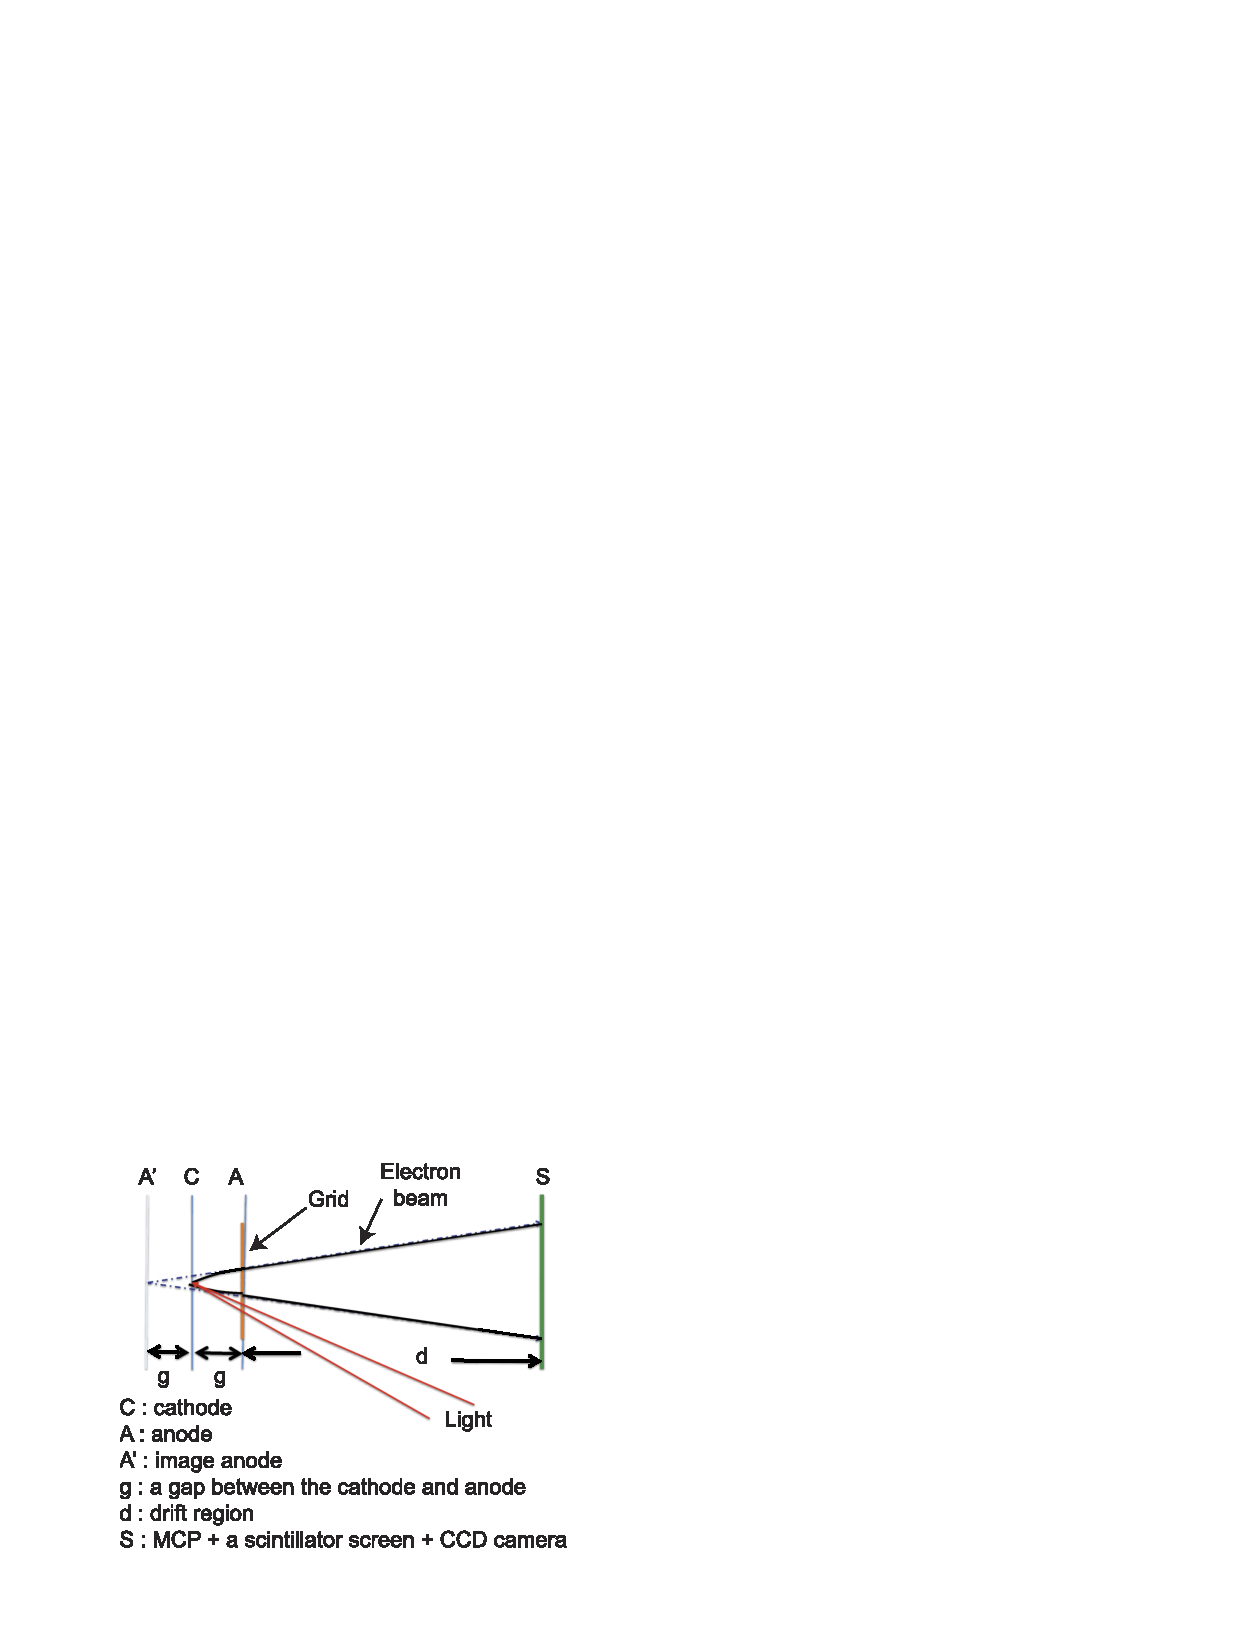
\includegraphics[width=0.6\textwidth]{free_expand}
\caption{\label{fig:free_expand} 自由膨胀法测量MTE的原理示意图}
\end{figure}

几个重要加速器应用的光阴极注入器出口束流参数最新测量值\cite{Zhou:2015aa,Krasilnikov:2012aa,prat2014emittance,Bartnik:2015aa}见表 \ref{tab:record-emit}。
\begin{table}[htbp]
\caption{几个重要装置注入器出口束流参数的实验测量结果}
\label{tab:record-emit}
\centering
\begin{tabular}{lcccccl}
\toprule
波段 & 峰值场强 & 发射场强 & 枪电压 & 发射度 & 峰值流强 & 装置 \\
 & MV/m & MV/m & MV & $\mu$m & A & \\
\midrule
S-band & $\sim$ 100 & $\sim$ 50 & $\sim$ 5 & $\sim$ 0.2--0.45 & 20--50 & LCLS/PSI \\
L-band & $\sim$ 60 & $\sim$ 45 & $\sim$ 7 & $\sim$ 0.3 & 15 & PITZ \\
DC & $\sim$ 4 & $\sim$ 4 & $\sim$ 0.4 & $\sim$ 0.6 & 30 & Cornell \\
VHF & $\sim$ 20 & $\sim$ 20 & $\sim$ 0.8 & $\sim$ 0.45 & 30 & APEX \\
\bottomrule
\end{tabular}
\end{table}

\section{论文工作的主要内容与创新点}
通过多年发展,光阴极出口处的束流发射度逐渐逼近热发射度,目前实验测量最优的结果是 200\,pC 电荷量下 \emit{0.2} 切片发射度及 \emit{0.3} 投影发射度\cite{Bettoni:2016aa}。200\,pC 束团的发射度是否已达到极限?我们的课题围绕这一问题进行探索,并尝试给出答案。如前所述,光阴极出口处束流发射度决定于初始束流热发射度,以及后续传输过程中对发射度的保持。束流在阴极表面产生时,阴极表面粗糙度对其贡献大小会影响后续的电子枪及注入器优化(抑制空间电荷效应发射度增长要尽量增大表面电场,但若表面粗糙度的横向电场发射度太大则增大表面电场会使热发射度增大,得不偿失),因此定量研究清楚一般阴极表面上粗糙度热发射度贡献大小对发射度优化有重要的意义;阴极上另一效应表面等离激元对束团亮度的影响不定,目前虽已有针对铜表面等离激元阴极的研究,但其它材料的发射属性依然未知,是否有新材料能够超越铜纳米阴极的亮度是一个值得探究的问题;阴极上的极限亮度已有公式给出,对于能够有效保持初始发射度到注入器尾端的扁平束和笔形束而言,若能从理论上预言其热发射度的极限,会对光阴极出口处发射度的优化有重要的参考意义;注入器的遗传算法优化表明要拉长初始束团可以抑制非线性空间电荷发射度增长,以降低注入器出口处发射度,但初始长度过长又会引入纵向非线性 RF 发射度,若能设法将非线性 RF 发射度补偿,就可能在注入器出口处获得更低(200\,pC 下 $\sim$ \emit{0.1})的发射度。论文工作主要围绕着以上几个问题逐步展开。

\subsection{论文工作的主要内容}
本论文主要内容如下:

(1)将点扩散函数的概念引入光阴极热发射度计算中,应用点扩散函数的观点给出了一般随机缓变粗糙表面阴极的表面离散效应和横向电场效应造成的粗糙度热发射度解析公式,并对一块真实阴极上光电发射过程中束团相空间及粗糙度热发射度的演化进行了数值模拟。模拟得到的真实阴极上的粗糙度热发射度与解析公式给出的符合较好。通过解析公式及数值模拟,发现对于三维随机缓变粗糙表面及粗糙度参数与其匹配的二维缓变粗糙表面,表面粗糙度对于发射度增长的贡献明显低于预期值。在阴极表面场强高达 120\,MV/m 时,发射度增长因子也低于 1.1,与发射度测量的一系列实验的测量值 1.5 $\sim$ 2 有较大差距。对于一块经过精细打磨的阴极(表面 rms 起伏不超过 \SI{30}{nm},表面 rms 坡度不大于 \SI{3}{mrad}),在阴极表面电场不太高($\sim$ 50\,MV/m)时表面粗糙度造成的发射度增长可以忽略不计。详细内容见第三章。

(2)模拟及实验探究了银纳米表面阴极的发射特性。先采用宽带反射率谱仪对表面刻有纳米结构的银晶片进行反射率谱测量,再将银晶片放入电子枪中进行高功率测试。银纳米表面晶片 266\,nm 激光下的量子效率 QE 测量值是 2.2$\times10^{-5}$,800\,nm 激光下的电子产额增益约为 400,x 向和 y 向的归一化热发射度分别为 1.6\,mm$\cdot$mrad/mm 和 1.7\,mm$\cdot$mrad/mm。多光子光电发射测量表明相同激光功率密度下,银纳米阴极相较于铜纳米阴极可以产生更高的电荷密度,但同时热发射度也要比铜纳米阴极大约 15\%。与平滑铜阴极相比,热发射度高了近一倍。我们也讨论了实验中观察到的一些有趣现象,如高功率测试后银纳米结构的损坏,离线反射率谱测量中 600\,nm 处奇怪的谐振峰,电子枪中由于 cathode-plug 设计造成的一系列效应等等。详细内容见第四章。

(3)理论计算了光阴极表面扁平束发射和笔形束发射两种情形下的极限热发射度,从极限热发射度的角度说明笔形束相对于扁平束的优势;针对笔形束发射中的非线性力导致的发射度增长问题,提出了分离型双频光阴极微波电子枪的概念,并用遗传算法对包含空间分离双频电子枪的注入器束线进行了多变量多目标优化。优化结果表明,在普通电子枪后引入一个高频腔可以将注入器出口处 \SI{200}{pC},峰值流强 \SI{30}{A} 的束流的发射度降低 $\sim$ 25\%,且切片发射度近乎与热发射度相等,这意味着双频电子枪成功将束流的初始横向亮度保持到注入器出口。当归一化热发射度降低至 \SI{0.5}{\mu m/mm} 时,优化器给出了注入器出口处流强 \SI{30}{A} 时切片发射度 $\sim$ \emit{0.10} 的方案。详细内容见第五章。

\subsection{论文工作的主要创新点}
本论文创新点如下:

(1)通过将点扩散函数引入光阴极热发射度计算,首次解析计算并数值模拟了真实粗糙表面阴极的粗糙度热发射度增长。理论及模拟结果表明,对于一块经过精细打磨的阴极(表面 rms 起伏不超过 \SI{30}{nm},表面 rms 坡度不大于 \SI{3}{mrad}),在阴极表面电场不太高($\sim$ 50\,MV/m)时表面粗糙度造成的发射度增长可以忽略不计。

(2)首次对银材料的纳米表面阴极发射属性进行了系统的高功率测量。实验结果表明银纳米阴极相较于铜纳米阴极可以产生更高的电荷密度,但同时热发射度也要比铜纳米阴极更大,因此适用于需要高电荷量且对发射度要求不太高的场景。

(3)首次理论上给出了扁平束发射和笔形束发射的极限热发射度,提出了采用分离型双频光阴极微波电子枪抑制非线性力发射度增长的方案,并用遗传算法进行了动力学优化验证。优化结果表明高频腔的引入可将光阴极的热发射度保持到注入器出口,并给出了注入器出口处流强 \SI{30}{A},切片发射度 $\sim$ \emit{0.10} 的方案。

%!TEX root = ../main.tex
\chapter{超低束流发射度实现的基础理论}
\label{chap:theory}

要探究光阴极微波电子枪中的极限束流发射度,首先要对光阴极电子枪中的物理有一个全面的认识,本章就来介绍光阴极电子枪中的基本物理概念与公式。

\section{束流相空间与束流发射度}
\subsection{束流相空间}
束流是由若干粒子组成的,每个粒子的运动状态都可以用一个六维向量来描述,即粒子的空间坐标 $(x, y, z)$ 和动量空间坐标 $(p_x, p_y, p_z)$ 的组合。那么在六维坐标系(相空间)中 $(x, y, z, p_x, p_y, p_z)$,每个粒子都可以用其中一个点代表。将束流中每个粒子都画在该坐标系中,就是束流的相空间分布。图 \ref{fig:phase-space} 给出了一个束团的相空间在横向竖向及纵向三对二维坐标系中的投影分布,这样的投影分布称为束流的二维相空间分布。
\begin{figure}[htbp]
\centering
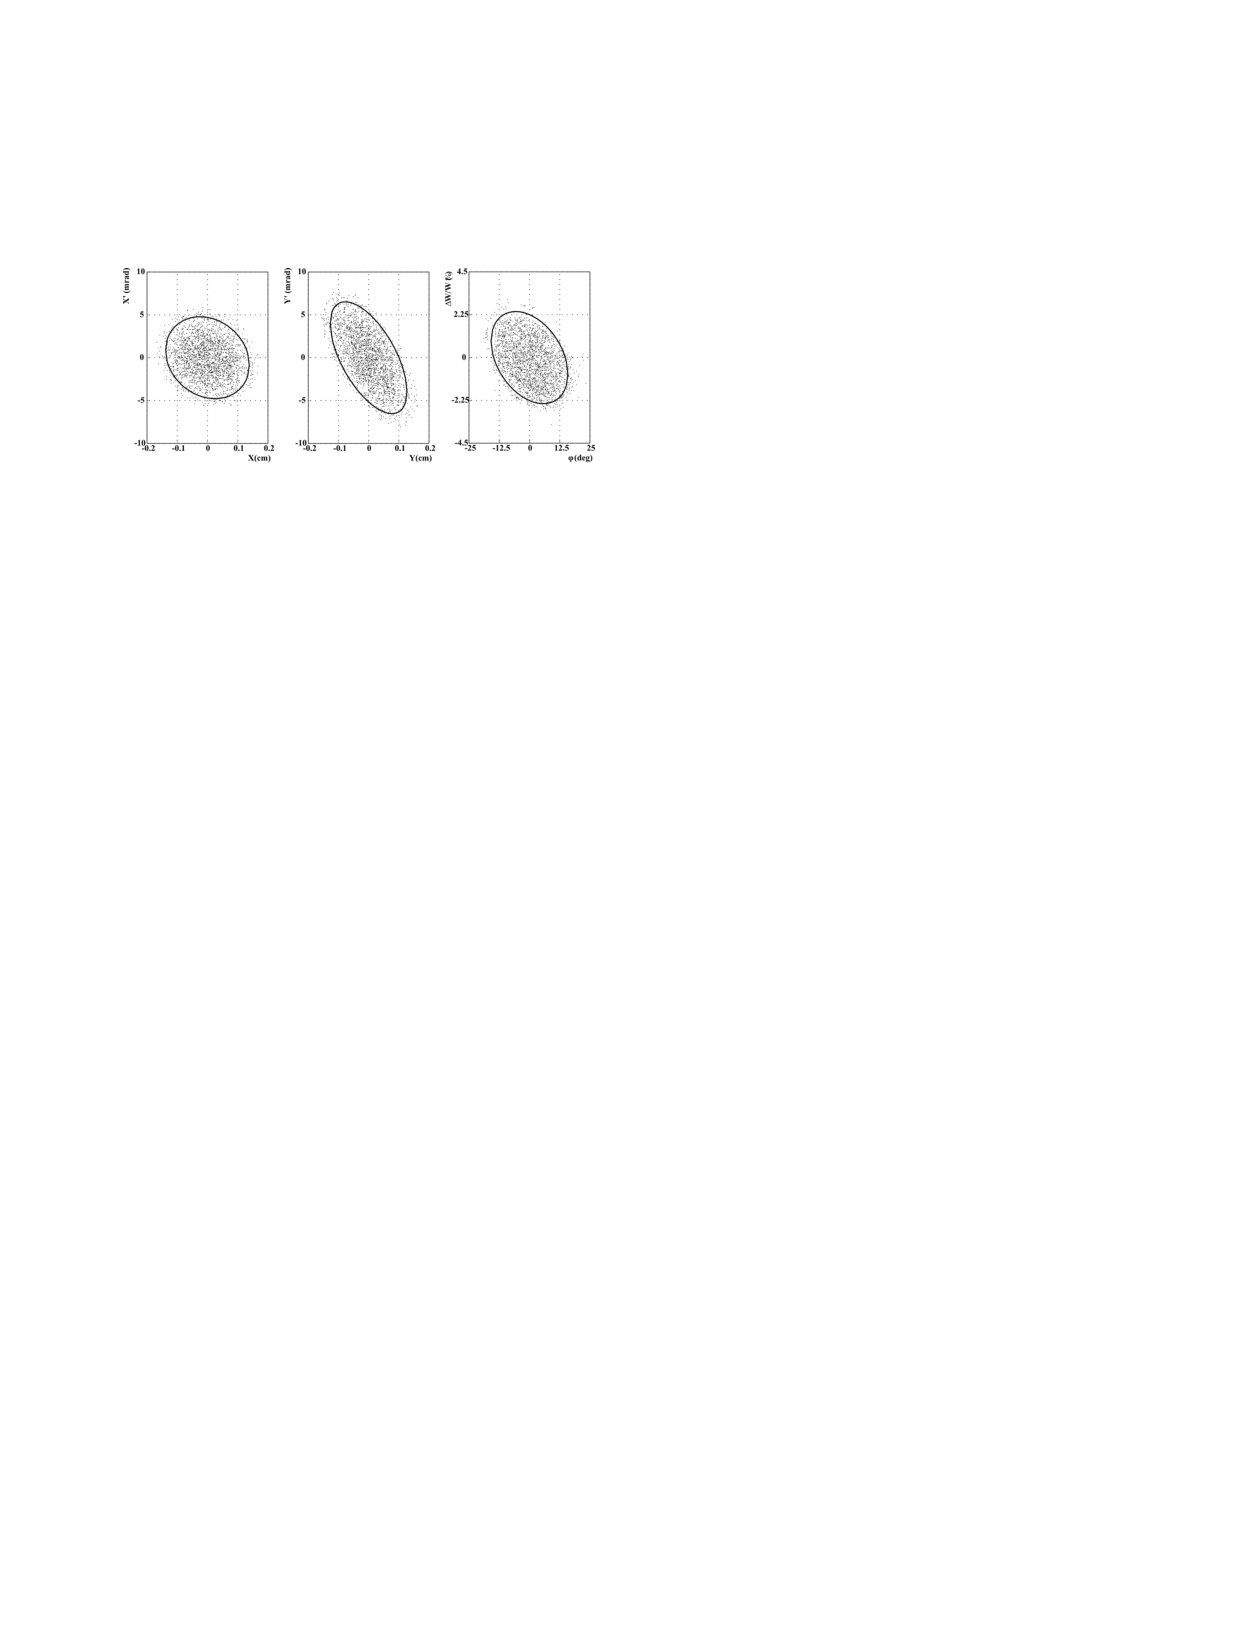
\includegraphics[width=0.9\textwidth]{phasespace}
\caption{\label{fig:phase-space} 一个束团在三方向的二维投影相空间分布\cite{yaramyshev2012new}}
\end{figure}

\subsection{束流发射度}
刘维尔定理指出,若粒子间无相互作用力,且束流所受外力均为保守力,则相空间的体积不变,这个不变的体积就称为束流的发射度。若束流的三方向无耦合(即三方向 $x, y, z$ 的运动互相无影响),则刘维尔定理也对三方向的二维相空间成立,此时三方向上的二维相空间的面积就称为相应方向的发射度。对于 x 方向的相空间分布,有下面的统计发射度定义:
\begin{equation}
\varepsilon = \sqrt{\langle x^2\rangle\langle p_x^2\rangle-\langle xp_x\rangle^2}
\label{eq:stat-emit-1}
\end{equation}
其物理意义是用椭圆去拟合相空间分布,求出的椭圆面积除以 $\pi$ 就是该相空间分布的发射度。由于该定义通过二阶矩(均方根)来进行统计平均,因此式 \ref{eq:stat-emit-1} 定义的发射度也称为均方根发射度。

在加速器物理中,由于束流中粒子之间存在空间电荷力,刘维尔定理不能精确成立;然而加速器中的束团普遍具有较好的柱对称性,以及束团中粒子数极为巨大,可近似将束流看做连续体,所以粒子的空间电荷效应往往可以等效成一个保守外力,在这种情况下,束流的发射度依然近似为常数。

\section{光阴极微波电子枪中存在的束流发射机制}

\subsection{光电发射}
光电效应是指光束照射在金属表面会使其发射电子的物理现象,发射出的电子被称为光电子。对于特定金属而言,激光功率密度不太大时,入射光光子能量必须大于某特定能量才能产生光电效应,该特定能量称为该金属的逸出功,这就是线性光电效应。线性发射时光电效应的发生与否与入射光强度没有关系;在激光功率密度较大时会发生非线性光电效应,此时入射光光子能量即使低于金属逸出功也能够发射光电子,非线性光电效应的光电流密度与入射光功率密度呈多项式关系。光电效应是一种量子效应,无法用 Maxwell 体系的经典电磁理论解释,必须借助光量子的概念才能解释。

光电效应(线性)可用下面的公式描述:
\[
E = h\nu-\phi
\]
其中$E$是出射光电子最大能量,$h\nu$为入射光子能量,$\phi$称为金属的逸出功或功函数(work function)。

\subsubsection{单光子光电效应与多光子光电效应}
人们在刚刚认识光电效应本质时,认为只有光子能量高于金属逸出功的时候才能产生光电发射。随着激光技术的发展,高功率激光被应用于研究中,此时发现了高阶光电效应:光子能量低于金属逸出功时,只要激光功率足够强,也能产生光电发射,这就是多光子光电效应现象。类似于单光子观点效应,多光子光电效应可用下面的公式描述:
\[
E = nh\nu-\phi
\]
其中$E$是出射光电子最大能量,$h\nu$为入射光子能量,$n$ 是光电效应阶数,$\phi$为金属的逸出功。下面详细介绍单光子光电效应和多光子光电效应的物理图像和重要结论。

单光子光电效应就是金属内电子吸收单个光子的光电效应。金属内处于费米能级(Fermi Energy)以下的束缚态电子吸收单个光子跃迁到高能态,进而成为自由电子向四周运动;经过若干次散射(能量损失)后部分高能态电子会到达金属表面,其中又有部分电子具有足够能量,克服金属表面势垒后从金属表面逸出,成为光电子。

1931 年 R. Fowler 研究了光电发射中光电流随入射光子能量变化曲线的拖尾现象\cite{Fowler:1931aa}。他采用简并电子气的观点,并假设:
	\begin{enumerate}
	\item 吸收光子后电子的能量略高于克服表面势垒所需能量,因此忽略电子间散射作用
	\item 所有沿阴极法向的动能与吸收的光子能量之和大于克服阴极表面势垒所需能量的电子都可从表面逃逸,这种电子叫做可出射电子
	\item 光电流正比于可出射电子数
	\end{enumerate}
	根据以上假设,R. Fowler 获得了光电发射电流 $I$ 的表达式,成功地揭示了拖尾现象的机理。1933 年 L. Dubridge 扩充了 Fowler 的理论,计算了光电发射中光电子的能谱\cite{DuBridge:1933aa},因此该理论被称为 Fowler-Dubridge 理论。

Fowler-Dubridge 理论中光电流可以简单推导如下:假定阴极表面法向沿 $+x$ 方向,利用简并电子气的速度分布公式,可以得到电子密度随 $x$ 方向速度 $v_x$ 的分布如下:
	\[
	n(v_x) = \frac{4\pi kT}{m}\left(\frac{m}{h}\right)^2\log\{1+e^{(\mu-\frac{1}{2}mv_x^2)/kT}\}
	\]
其中 $k$ 是玻尔兹曼常数,$m$ 是电子静止质量,$T$ 是金属温度,$h$ 是普朗克常数,$\mu$ 为金属的费米能级。根据 Fowler 的第二条假设,单位体积内所有可出射的电子数为:
	\begin{eqnarray*}
	&N &= \int_{\frac{1}{2}mv_x^2=\phi_w+\mu-h\nu}^{\infty}n(v_x)dv_x\\
	&&= \frac{2\pi kT}{m}\left(\frac{2kT}{m}\right)^{1/2}\left(\frac{m}{h}\right)^3\int_0^{\infty}\frac{\log\{1+e^{-y+(h\nu-\phi_w)/kT}\}}{\{y+(\mu+\phi_w-h\nu)/kT\}^{1/2}}dy
	\end{eqnarray*}
	$y$ 远大于 1 时该积分分子趋于 0,因此仅有 $y$ 不太大时该分式才会对积分有主要贡献,此时分母中的 $y$ 相对于第二项(根据 Fowler 第一条假设,一般远大于 1)可以忽略,所以上式可简化为:
	\[
	N = \frac{2\sqrt{2}\pi m^{3/2}}{h^3}\frac{(kT)^2}{(\mu+\phi_w-h\nu)^{1/2}}\int_0^{\infty}\log\{1+e^{-y+(h\nu-\phi_w)/kT}\}dy
	\]
	令 $F(x) = \int_0^{\infty}\log(1+e^{-y+x})dy$,则:
	\[
	N = \frac{2\sqrt{2}\pi m^{3/2}}{h^3}\frac{(kT)^2}{(\mu+\phi_w-h\nu)^{1/2}}F\left(\frac{h\nu-\phi_w}{kT}\right)
	\]
	根据 Fowler 的第三条假设,光电流 $I$ 正比于可出射电子数 $N$,我们就得到单光子发射光电流:
	\begin{equation}
	I = CT^2F\left(\frac{h\nu-\phi_w}{kT}\right)
	\end{equation}
	其中 $C$ 为常数,$T$ 为电子气温度,$F(x)$ 为 Fowler 函数,可以展成下面级数:
	\[
	F(x) =
	\begin{cases}
	e^x-\dfrac{e^{2x}}{2^2}+\dfrac{e^{3x}}{3^2}-\cdots & x \le 0\\[10pt]
	\dfrac{\pi^2}{6}+\dfrac{x^2}{2}-\left[e^{-x}-\dfrac{e^{-2x}}{2^2}+\dfrac{e^{-3x}}{3^2}-\cdots\right] & x > 0
	\end{cases}
	\]
	Fowler 函数的特征是在 $x < 0$ 时,其值随 $x$ 的减小而迅速衰减。这个特性意味着波段合适的激光可以作为阴极的发射开关,即光电发射具有良好的可控性。

单光子光电发射中,光电子数目(光电子产额)与入射光强度成正比,因此又被称为线性光电效应,可以定义光阴极的量子效率 QE 如下:
	  \begin{equation}
	  QE = \frac{N_e}{N_p} = \frac{Q/e}{IS\tau/h\nu} = \frac{J}{I}\cdot\frac{h\nu}{e}
	  \end{equation}
	  其中$N_e$为出射光电子数,$N_p$为入射光子数,$Q$是出射束团电荷量,$J$是出射电流密度,$I$是入射光功率密度,$h\nu$为入射光子能量,$e$为电子电荷量,$S$为入射光横向面积,$\tau$为入射光脉宽

多光子光电效应就是金属内电子吸收多个光子的光电效应。金属内处于费米能级以下的束缚态电子同步或非同步吸收多个光子跃迁到高能态,进而成为自由电子向四周运动;经过若干次散射(能量损失)后部分高能态电子会到达金属表面,其中又有部分电子具有足够能量,克服金属表面势垒后从金属表面逸出,成为光电子。

	J. Bechtel 于 1973 年在他的博士论文(未发表)里推广了 Fowler-Dubridge 模型\cite{bechtel1975four,bechtel1977two},将多光子发射的情形包含进来,他得到多光子发射光电流密度:
\begin{equation}
J_n = \alpha_nA\left(\frac{e}{h\nu}\right)^n(1-R)^n\cdot I^nT^2F\left(\frac{nh\nu-\phi_w}{kT}\right)
\label{eq:multi-emission}
\end{equation}
其中 $A$ 为 Richardson 常数 \SI{120}{A.cm^{-2}.K^{-2}},$R$ 为阴极表面反射率,$I$ 为入射激光功率密度,$\alpha_n$ 是与 n-光子电离常数成正比的常数。
	
	取 $n=0$,此时 $\alpha_0 = 1$,我们就得到热发射电流密度公式;取 $n=1$,我们就得到单光子光电流密度公式。
	于是总发射电流密度为:
	\begin{equation}
	J = \sum_{i = 0}^{\infty}J_i
	\end{equation}
	此公式包含了热发射电流,线性光电流和高阶光电流。

对于多光子光电发射,光电子产额与入射光强度成幂函数关系,因此又被称为高阶光电效应或非线性光电效应;N光子光电效应的光电流密度J与入射光强度I成N次幂关系:
\[
J \propto I^N
\]
由于单个光子激发电子的数目与激光功率密度有关,在高阶光电效应中不能再用量子效率来描述光电发射的电子产额大小。

\subsubsection{表面等离激元加强的光电发射}
Maxwell 电磁理论预言在两种介电常数实部反号的介质的交界面存在一种沿交界面传播的电磁-电荷密度振荡波,也称做表面等离激元(Surface Plasmon Polaritons, SPPs)\cite{Ritchie:1957aa,Barnes:2003aa,Maier:2007ab,Pitarke:2007aa}。利用经典的 Drude 模型可导出金属的介电常数实部为负,因此金属与介质交界面可以存在 SPPs。

表面等离激元有下面特点:1)SPPs 存在一个频率上限($\omega_P/\sqrt{2}$),低于此频率的光才能激发 SPPs;2)入射光必须设法增加横向动量(横向波数)才能激发 SPPs;3)SPPs 沿交界面传播,垂直于交界面衰减;4)特定波长和角度入射的光可被 SPPs 完全共振吸收,此时交界面处会形成极高电场。SPPs 的物理图像及具体性质会在第四章中详细介绍。

由于 SPPs 有提高入射光吸收率/增强阴极表面光场的性质,可以利用 SPPs 来加强光电发射,提高阴极的量子效率\cite{Tsang:1991aa,Neo:2012aa,Grubisic:2012aa,Polyakov:2013ab,Li:2013aa}。

\subsection{热发射}
热发射即因金属表面电子热运动而产生的电子发射。对于温度高于绝对零度的金属,假定其温度为 $T$($T > 0$),由于金属内部的电子能量服从 Fermi-Dirac 分布($T$ 较小时近似 Maxwell-Boltzmann 分布),其拖尾部分的电子处于较高能态,从而具有足够的能量克服金属表面势垒,逸出金属表面\cite{richardson1901negative}。

阴极上的热发射电流密度可以利用 Drude-Sommerfeld 模型中的电子速度分布公式做近似直接导出如下。金属表面的电子速度分布遵守:
	\[n(v_x, v_y, v_z) = 2\left(\frac{m}{h}\right)^3\frac{1}{e^{(E-E_F)/kT}+1}\]
	由于只有动能 $E$ 远高于费米能级 $E_F$ 的电子才能克服金属表面势垒 $U$ 逸出,我们统计热电流时可将 Fermi-Dirac 分布近似为 Maxwell-Boltzmann 分布:
	\[\frac{1}{e^{(E-E_F)/kT}+1} \rightarrow e^{-(E-E_F)/kT}\]
	假定阴极法向沿 $+x$ 方向,那么热发射电流密度 $J$ 可写成:
	\[J = \iiint\limits_{mv_x^2/2 > U}\zskip ev_xn(v_x, v_y, v_z)dv_xdv_ydv_z\]
	将近似后的电子速度分布公式代入,利用高斯积分:
	\[\int_{-\infty}^{\infty}e^{-\alpha z^2}dz=\sqrt{\frac{\pi}{\alpha}}\]
	可以得到:
	\[J = \frac{4\pi emk^2}{h^3}T^2\exp\left(\frac{E_F-U}{kT}\right)\]
	由此我们得到热发射电流密度公式:
\begin{equation}
	J = AT^2\exp\left(-\frac{\phi}{kT}\right)
\end{equation}
	其中 $A=4\pi emk^2/h^3\approx \SI{1202}{\micro A.\milli m^{-2}.K^{-2}}$,称为Richardson常数;$\phi=U-E_F$,定义为金属的逸出功,$k$ 是 Boltzmann 常数。

热发射可以看作是零阶光电发射,电子吸收 0 个光子而逸出金属表面,电子逃逸是通过热运动完成的。热发射特点如下:1)热发射电流只与金属温度$T$有关,与入射光强度大小无关;2)热发射电流的强度很小,在 $T = \SI{300}{K}$ 时热发射电流在 \SI{1}{\mu A} 量级。

\subsection{场致发射(暗电流)}
场致发射即因金属表面存在很强的电场而产生的电子发射。当金属表面存在很强的引出电场时,金属表面势垒会在电场的影响下变成准三角形,其厚度变小,从而金属表面的电子可以通过量子隧穿效应穿越表面势垒,逸出金属表面。其物理图像参见示意图 \ref{fig:fieldemission}。
\begin{figure}[htbp]
\centering
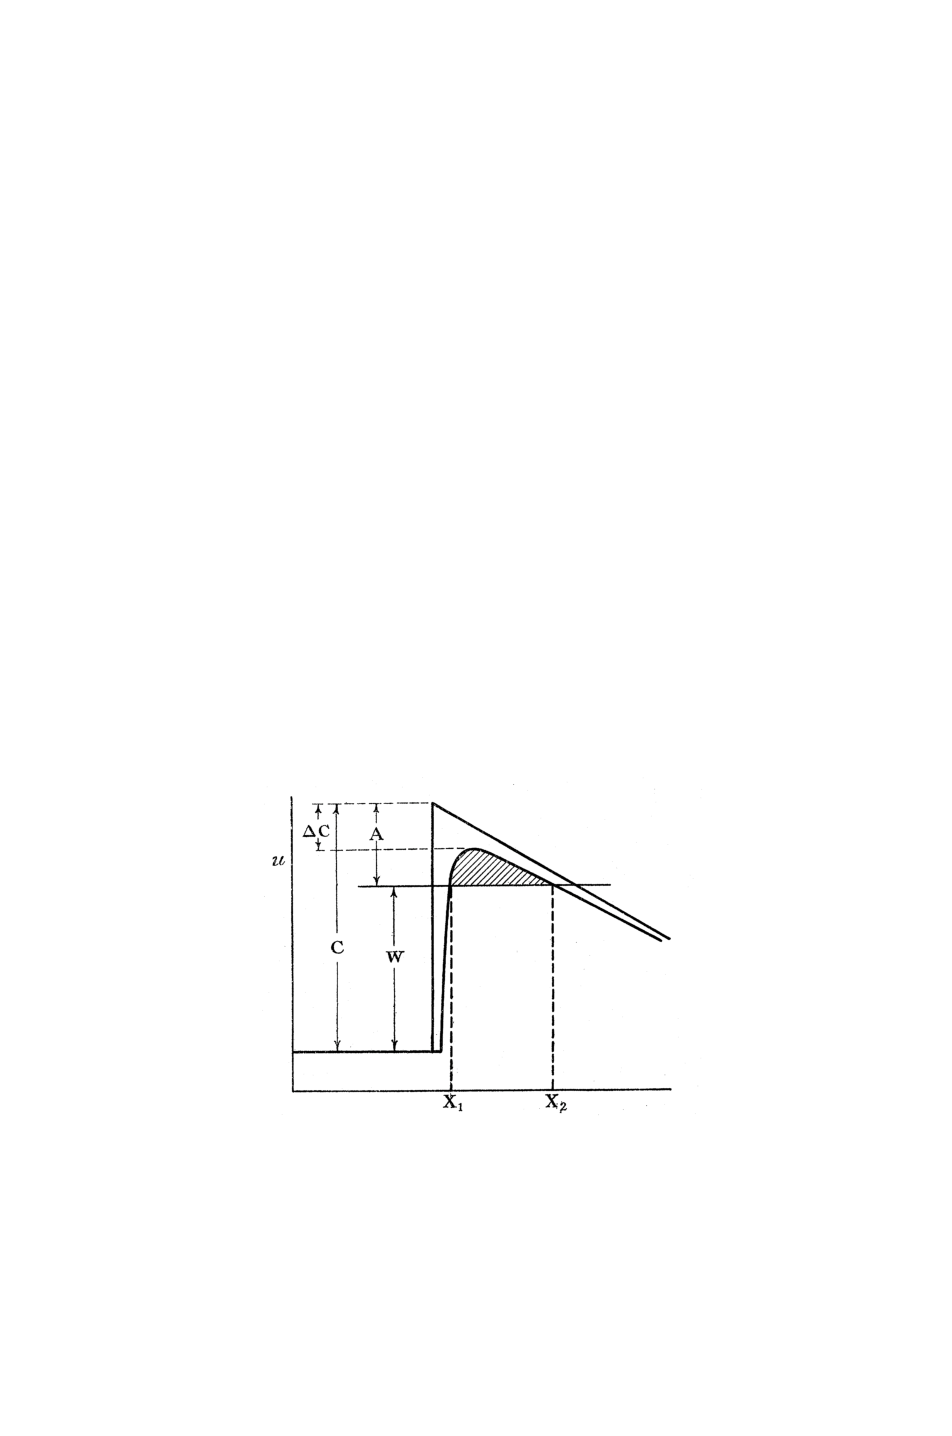
\includegraphics[width=0.6\textwidth]{fieldemission}
\caption{\label{fig:fieldemission} 场致发射示意图\cite{nordheim1928effect}。}
\end{figure}

在光阴极领域,阴极表面场致发射产生的电流又被称为暗电流。暗电流密度可以通过量子理论给出。考虑阴极表面附近的电子,假定阴极法向沿 $+x$ 方向,利用简并电子气的电子速度分布 $n(v_x, v_y, v_z)$,可写出场致发射电流密度为:
	\[
	J = \iiint\limits_{v_x \in [0, +\infty]}\zskip ev_xn(v_x, v_y, v_z)\cdot \Theta(v_x)dv_xdv_ydv_z
	\]
	其中 $\Theta(v_x)$ 为 $x$ 方向速度为 $v_x$ 的电子的隧穿概率。接下来采用 WKB 近似(WKB (Wigner, Kramers, Brillouin) approximation)来计算量子隧穿概率。

	假定阴极法向沿 $+x$ 方向,我们计算阴极表面势垒分布为 $V(x)$ 情形下的电子波函数,从而得到隧穿概率。设此时电子波函数为 $\Phi(x)$,利用一维含时 Schr\"odinger 方程,我们有:
	\[\frac{d^2\Psi}{dx^2}=\frac{2m(V-E_x)}{\hbar^2}\Psi\]
	其中 $E_x$ 为电子在 $x$ 方向的动能。考虑在 $[x, x+dx]$ 一段的势垒 V,我们近似认为其为常数,那么可解出波函数 $\Phi$ 在此区间满足:
	\[\Phi(x+dx)=\Phi(x)\exp\left(-\frac{\sqrt{2m[V(x)-E_x]}}{\hbar}dx\right)\]
	于是 $\Psi$ 在整个 $x$ 正半轴上的可写为:
	\[\Phi(x)=\Phi(0)\exp\left(-\int_0^x\frac{\sqrt{2m[V(s)-E_x]}}{\hbar}ds\right)\]
	上面的公式就称为 WKB 近似。有了波函数,我们便可以计算特定形状势垒下的隧穿概率:
	\[\Theta(E_x)=\frac{\Psi(L)\Psi^*(L)}{\Psi(0)\Psi^*(0)}=\exp\left(-\frac{2\sqrt{2m}}{\hbar}\int_0^L\zskip\sqrt{V(s)-E_x}ds\right)\]
	式中 $L$ 为势垒宽度,也即相对(能量 $E_x$ 的)势垒高度刚好等于 0 的位置。下面以外场为恒定电场且不考虑空间电荷力时的三角(ET,Exact Triangular)势垒为例计算隧穿概率。
	假定外场梯度为 $F$,那么 $V(x)-E_x=\phi-eFx$,其中 $\phi$ 为相对电子 $x$ 方向动能 $E_x$ 的势垒高度,此时势垒宽度 $L=\phi/eF$。代入 $\Theta$ 的计算公式,就得到 ET 势垒的隧穿概率:
	\begin{equation}
	\Theta(E_x)=\exp\left(-\frac{4\sqrt{2m}}{3e\hbar}\frac{\phi(E_x)^{3/2}}{F}\right)
	\end{equation}
	其中 $\phi(E_x)=\phi_w+E_F-E_x$,是相对于 $x$ 方向动能为 $E_x$ 的电子的金属表面势垒高度。
	
	有了隧穿概率,将其代回到场致发射电流密度公式中就可以获得暗电流密度。

	容易将场致发射电流密度公式化为下面形式:
	\[J = A\cdot\frac{T}{k}\int_0^{\infty} dE_x\Theta(E_x)\ln\left(e^{-\frac{E_x-E_F}{kT}}+1\right)\]
	其中 $A$ 为 Richardson 常数。考虑到场致发射电子大部分能量在 Fermi 能级附近,我们可以将一般形式的 $\Theta(E_x)$ 在 $E_F$ 附近做 Taylor 展开到二阶,有:
	\[\Theta(E_x)=\Theta(E_F)\cdot e^{\left(\frac{2\sqrt{2m}}{\hbar}(E_x-E_F)\int\limits_0^L\frac{ds}{\sqrt{V(s)-E_F}}\right)}\]
	将上式代入 $J$ 的表达式,考虑到场致发射电流主要由 $E_x$ 在 Fermi 能级附近的电子贡献,可以将 $J$ 中的积分区间扩充至 $(-\infty, \infty)$。
	通过变量代换及积分公式:
	\[\int_0^{\infty}du u^{-\alpha-1}\ln(u+1)=\frac{\pi}{\alpha\sin(\alpha\pi)},\quad\mathrm{Re}(\alpha)\in(0, 1)\]
	可得到:
	\[J = AT^2\frac{\Theta(E_F)}{C^2\mathrm{Sa}(C\pi)}\]
	其中 $C$ 满足:
	\[C = kT\frac{\sqrt{2m}}{\hbar}\int_0^L\frac{ds}{\sqrt{V(s)-E_F}}\]
	代入 ET 势垒的隧穿概率的相关计算结果,最终我们有场致发射电流密度:
	\begin{equation}
	J=\frac{AF^2}{\phi_w}\exp\left(-\frac{B\phi_w^{3/2}}{F}\right)\frac{1}{\mathrm{Sa}(CT\phi_w^{1/2}/F)}
	\end{equation}
	其中 $A=e^3/8\pi h$,$B=4\sqrt{2m}/3e\hbar$,$C=2\pi k\sqrt{2m}/e\hbar$
	当温度 $T\rightarrow \SI{0}{K}$ 时,$\mathrm{Sa}$ 函数趋近于 1,由此我们有 Fowler-Nordheim 公式:
	\begin{equation}
	J=\frac{AF^2}{\phi_w}\exp\left(-\frac{B\phi_w^{3/2}}{F}\right)
	\end{equation}
	其中 $A=e^3/8\pi h\approx\SI{1.541e-6}{A.eV.V^{-2}}$,$B=4\sqrt{2m}/3e\hbar\approx\SI{6.831}{eV^{-3/2}.V.\nano m^{-1}}$,$F$ 是金属表面场梯度。

场致发射也可以看作是零阶光电发射,电子吸收 0 个光子而逸出金属表面,电子逃逸通过量子隧穿效应完成。场致发射有下面特点:1)场致发射电流对金属温度 $T$ 的变化不敏感;2)场致发射电流随引出电场的梯度下降而迅速减小。

\section{光阴极微波电子枪中束流的初始发射度}
第一节中已介绍了束流发射度的概念,将其应用于电子枪光阴极表面,就是光阴极微波电子枪中束流的初始发射度(intrinsic emittance)。由于其主要是因为电子的热运动造成,也称为热发射度(thermal emittance)。

\subsection{初始发射度(热发射度)}
\subsubsection{三步模型}
Fowler-Dubridge 模型仅仅考虑了阴极中电子在吸收光子后的运动状态,而未考虑光子吸收和电子输运的过程,因此无法用于计算光电子束较细致的参数,例如量子效率 QE 和发射度。1958 年 W. Spicer 开发了三步模型,考虑光子吸收和电子输运的过程,成功计算了 QE\cite{spicer1958photoemissive};2006 年 D. Dowell 利用三步模型,进行了简化并给出了 QE 和发射度的非常简洁的公式,并被实验所验证\cite{Dowell:2006aa}。

电子发射的三步模型即下面的三步:
	\begin{enumerate}
	\item 光子激发(Excitation)阴极内电子
	\item 电子输运(Transport)到阴极表面
	\item 电子逃逸(Escape)到真空
	\end{enumerate}
	
第一步是光子激发阴极内电子:假设能量为 $h\nu$ 的光子垂直入射光滑金属阴极(沿 $-z$ 方向入射),由于光子被金属中电子吸收是一个泊松过程,因此光子被吸收的概率会随入射深度 $s$ 呈指数衰减,也即:
	\[
	p(\gamma: \mathrm{surface} \to s) = \frac{1}{\lambda_p}e^{-s/\lambda_p}
	\]
	其中 $p(\gamma: \mathrm{surface} \to s)$ 是进入阴极表面的光子在入射深度 $s$ 处被吸收的概率密度,$\lambda_p$ 是该能量光子在金属中的平均自由程。而能量为 $E$ 的电子吸收该光子,从而从能级 $E$ 跃迁到 $E+h\nu$ 的概率正比于能级 $E$ 的电子数与能级 $E+h\nu$ 的空位数的乘积:
	\[
	p(e^{-}: E\to E+h\nu) \propto f_{\mathrm{FD}}(E)g(E)\cdot [1-f_{\mathrm{FD}}(E+h\nu)]g(E+h\nu)
	\]
	其中 $f_{\mathrm{FD}}(E)$ 为 Fermi-Dirac 分布,$g(E)$ 是能级 $E$ 处的能态密度。
	
第二步是电子输运到阴极表面:被激发到高能态 $E+h\nu$ 的电子开始输运过程。假设被激发的电子运动方向随机,并在 $4\pi$ 方向角均匀分布,再限定被激发的电子能量仅略高于有效逸出功,则电子输运到阴极表面的概率等于电子朝向阴极表面运动并输运过程中无散射的概率(一旦发生散射电子丢失能量,剩余能量不足以克服有效势垒),也即:
	\[
	p(e^{-}: (E+h\nu, s, \theta) \to \mathrm{surface}) = e^{-s/(\lambda_{e-e}(E+h\nu)\cos\theta)}
	\]
	其中 $\lambda_{e-e}(E+h\nu)$ 是能量为 $E+h\nu$ 电子的散射平均自由程,$\theta$ 为电子运动方向与阴极表面法向($+z$)的夹角。
	
第三步是电子逃逸到真空:能量为 $E+h\nu$ 的电子以 $\theta$ 角传输至阴极表面时会尝试克服表面势垒而逃逸。假设所有 $+z$ 方向动能大于等于有效势垒高度(有效逸出功与 Fermi 能量之和)的电子都可以逃逸,可得逃逸概率为:
	\[
	p(e^{-}: \mathrm{escape}) = u[(E+h\nu)\cos^2\theta-\mu-\phi_{\mathrm{eff}}]
	\]
	其中 $u(x)$ 为阶跃函数:$x\ge 0$ 时 $u(x)=1$;$x<0$ 时 $u(x)=0$,$\mu$ 为 Fermi 能量。

\subsubsection{热发射度与量子效率}
利用上小节所述的三步模型及公式,可以计算光阴极的量子效率\cite{Dowell:2009ab}:
\begin{equation}
	\mathrm{QE}(\omega) \approx\dfrac{1-R(\omega)}{1+\dfrac{\lambda_{\mathrm{opt}}}{\bar{\lambda}_{e-e}(\omega)}}\frac{(\hbar\omega-\phi_{\mathrm{eff}})^2}{8\phi_{\mathrm{eff}}(E_F+\phi_{\mathrm{eff}})}
\end{equation}
以及光阴极的热发射度\cite{Dowell:2009ab}:
\begin{equation}
	\varepsilon_{n} =\sigma\sqrt{\dfrac{\hbar\omega-\phi_{\mathrm{eff}}}{3mc^2}}
	\label{eq:emit-dowell}
\end{equation}

\subsection{阴极材料与激光参数对热发射度的影响}
\subsubsection{空间电荷限}
	C. Child 于 1911 年提出 Child 定律\cite{Child:1911aa},该定律是说在平行两极板间的电压 $V$ 固定的情况下,其极板间电流密度存在最大值 $J$,并且 $J$ 与 $V$ 成 3/2 次方关系,因此又被称为 3/2 次方定律。1911 年发表的情况针对的是离子流,I. Langmuir 在 1913 年将 Child 的方法应用于电子流\cite{langmuir1913effect},因此该定律又被称为 Child-Langmuir 定律。

	阴极上空间电荷限的本质是:在两极板间的电流产生的空间电荷场会减小发射极的引出电场,当电流大到一定程度时,发射极表面的总引出电场降到 0,逸出的电子无法获得加速,发射电流无法进一步增加,因此电压固定时发射电流存在饱和值。
	
	Child-Langmuir 模型的假定如下\cite{Child:1911aa,langmuir1913effect,Langmuir:1923aa}:
	\begin{itemize}
	\item 不考虑相对论效应
	\item 忽略极板间运动的粒子间的散射
	\item 极板间的粒子是同一的(同质量,同电荷量)
	\item 阴极上的初始发射速度为 0
	\end{itemize}
	那么当两极板间电流处于稳态时,可以直接利用 Poisson 方程导出空间电荷限电流公式。考虑两极板间电流中的一点,那么有 Poisson 方程成立:
	\[\nabla^2V=-\frac{\rho}{\epsilon_0}\]
	其中 $V$ 为该点电势,$\rho$ 为该点电荷密度。
	由于阴极上($V=0$)粒子的初始动能为 0,根据能量守恒,电势 $V$ 处粒子的能量满足:
	\[\frac{1}{2}mv^2+qV=0\]
	考虑到电荷守恒及稳态条件,有:
	\[\nabla\cdot\vec{J}=-\frac{\partial \rho}{\partial t}= 0\]
	而电流密度$\vec{J}$满足:
	\[\vec{J}=\rho \vec{v}\]
	仅考虑一维情形(束流沿 $z$ 轴运动),可知 $J$ 是个常量,联立以上各式可得关于电势 $V$ 的方程:
	\[\frac{d^2V}{dz^2}+AV^{-\frac{1}{2}}=0\]
	其中 $A=-\frac{J}{\varepsilon_0}\sqrt{-m/2q}$。解上面方程并代入边界条件:
	\begin{eqnarray*}
	&&V|_{z=0}=0\\
	&&V|_{z=d}=V_d
	\end{eqnarray*}
	可得电压$V_d$与最大电流密度 $J$ 之间的关系为:
	\[J = \frac{4\varepsilon_0}{9}\sqrt{-2q/m}\cdot \frac{V_d^{\frac{3}{2}}}{d^2}\]
	对于电子而言,得到阴极上的空间电荷限电流密度为($V_d\rightarrow V$):
	\begin{equation}
	J = \frac{4\varepsilon_0}{9}\sqrt{2e/m}\cdot \frac{V^{\frac{3}{2}}}{d^2}
	\end{equation}

	在带有电子枪的电子器件中,定义导流系数 $P=I/V^{3/2}$,该系数衡量电子枪的发射能力,$P$ 的单位为朴(P)。一般微波器件的电子枪,导流系数在 \SIrange[range-phrase = --]{0.1}{1}{\micro P} 的范围。导流系数反映了阴极发射电流$I$与阴阳极间电压$V$之间的关系,它仅取决于枪的几何尺寸。

\subsection{阴极表面状况与阴极表面 RF 场对热发射度的影响}
真实阴极并非一个完美的平面,而是一个有起伏的粗糙表面。粗糙表面的起伏会造成光电子发射方向的离散,且阴极表面的 RF 场会在起伏表面上产生横向电场分量,造成光电子横向动量的增加,这都会对光阴极热发射度产生一定影响。人们目前采用理想二维($x$ 和 $z$)正弦表面来定性给出粗糙度对热发射度造成的影响\cite{He:2004aa,Krasilnikov:2006aa}。设二维正弦表面的表面形态函数 $R(x)$ 为:
\[
	R(x) = a\cos(kx)
\]
下面来简单推导表面离散和横向电场造成的发射度增长。
\subsubsection{表面离散热发射度}
假定光电子以表面法向为中心发射,其动量分布与平面情形下相同,那么有:
\[
\left(\begin{array}{c}
p_x\\
p_z
\end{array}\right)=
\left(\begin{array}{cc}
\cos\theta & -\sin\theta\\
\sin\theta & \cos\theta 
\end{array}\right)
\left(\begin{array}{c}
p_x^{\prime}\\
p_z^{\prime}
\end{array}\right)
\]
其中 $\theta$ 是从 z 轴到点 \textbf{P} 法向的夹角,且 $p_x^{\prime}, p_z^{\prime}$ 分别是发射电子在局部坐标系下的横向和纵向动量。利用发射度统计公式 \ref{eq:stat-emit-1},设 $\xi=ak$,就有:
\begin{equation}
\Delta^2 = \Delta_{0}^2\left(1+\frac{1}{2}\xi^2\right)
\end{equation}
其中 $\Delta$ 为归一化散角,即 $\sqrt{\langle p_x^2\rangle}/mc$。

\subsubsection{横向电场热发射度}
当 $\xi=ak\ll 1$ 时,设平均外加电场为 $E$,则阴极表面电场可以如下近似描述:
\begin{eqnarray*}
E_x &=& E\xi\cdot e^{-kz}\sin kx \\
E_z &=& E\left(1+\xi e^{-kz}\cos kx\right)
\end{eqnarray*}
由于刚出射的电子还是非相对论粒子,可以直接用经典力学写出粒子运动方程:
\begin{eqnarray*}
\ddot{x} &=& \frac{eE}{m}\xi\cdot e^{-kz}\sin kx \\
\ddot{z} &=& \frac{eE}{m}\left(1+\xi e^{-kz}\cos kx\right)
\end{eqnarray*}
做近似:
\begin{itemize}
\item 认为电子出射方向近似是 $z$ 向
\item 极短的运动过程中横向位置 $x$ 基本不发生改变
\end{itemize}
令 $eE/m=A$,积分上面第一式,有:
\[
	\dot{x}_{\infty} - \dot{x}_0 \approx A\xi\sin kx\int_0^{\infty}\zskip e^{-kz}\,dt
\]
考虑到 $\xi \ll 1$,$z$ 向运动方程可以近似为:
\[
\ddot{z}\approx A
\]
因此 $z$ 和 $t$ 的关系就可以直接积分得到:
\[
z\approx \dot{z}_0 t + \dfrac{1}{2}At^2
\]
将上式代入横向速度方程,就得到:
\[
	\dot{x}_{\infty} - \dot{x}_0 \approx A\xi\sin kx\int_0^{\infty}\zskip e^{-k\left(\dot{z}_0 t + \frac{1}{2}At^2\right)}\,dt
\]
由于电子初始纵向速度 $\dot{z}_0$ 很小,忽略指数上时间的线性项,直接由高斯分布积分公式得到:
\[
	\dot{x}_{\infty} - \dot{x}_0 \approx \sqrt{\frac{\pi A}{2k}}\cdot\xi\sin kx
\]
因此归一化散角 $\Delta_{\infty}$ 就满足:
\begin{eqnarray*}
\Delta_{\infty}^2 &=& \frac{\left\langle\dot{x}_{\infty}^2\right\rangle}{c^2} \approx \frac{\left\langle\left(\dot{x}_0 + \sqrt{\frac{\pi A}{2k}}\cdot\xi\sin kx\right)^2\right\rangle}{c^2} \\
	&=& \frac{\left\langle\dot{x}_{0}^2\right\rangle}{c^2} + 2\sqrt{\frac{\pi A}{2k}}\xi\frac{\left\langle\sin kx\cdot\dot{x}_{0}\right\rangle}{c^2} + \frac{\pi A}{2k}\xi^2\frac{\left\langle\sin^2 kx\right\rangle}{c^2}
\end{eqnarray*}
若假定交叉项为 0,那么上式可化为:
\[
	\Delta_{\infty}^2 \approx \Delta_{0}^2 + \frac{\pi A\xi^2}{4kc^2}
\]
将 $A,\xi$ 的表达式代回上式,再代入均方根发射度公式,就得到:
\[
	\varepsilon^2 \approx \varepsilon_{0}^2 + \frac{\pi e}{4mc^2}\cdot \sigma^2a^2kE
\]
其中 $\sigma$ 是激光横向 rms 尺寸。上式右边第二项的平方根便是横向电场对热发射度的贡献,其大小与外加电场强度的平方根成正比。

\subsubsection{肖特基效应}
	电子在逃逸出金属阴极表面时要克服表面势垒(真空势垒和镜像电荷势的总和)的作用;阴极表面的高引出场强会降低表面势垒的高度,从而降低电子所感受到的逸出功,这种效应叫做 Schottky 效应\cite{tersoff1984schottky},电子所感受的逸出功叫做有效逸出功。

	对于单个电子而言,在金属阴极表面距离 $x$ 的位置,其电势能为:
	\[
	\Phi = \phi_{\mathrm{w}} - \frac{e^2}{16\pi\varepsilon_0x} - eE_0x
	\]
	其中 $\phi_{\mathrm{w}}$ 为金属的逸出功,$-e^2/16\pi\varepsilon_0x$ 是镜像电荷势能,$- eE_0x$ 是引出场势能。
	容易看出总势能在距离 $x$ 满足:
	\[
	x = \sqrt{\frac{e}{16\pi\varepsilon_0E_0}}
	\]
	时取得最大值,最大值即为有效逸出功:
	\begin{equation}
	\phi_{\mathrm{eff}} = \phi_{\mathrm{w}} - e\sqrt{\frac{eE_0}{4\pi\varepsilon_0}}
	\end{equation}
由于肖特基效应的存在,由发射度公式 \ref{eq:emit-dowell},表面电场的存在会增大束流发射度。

\subsection{高阶光电流对热发射度的影响}
高阶光电流的发射度可以写做:
\begin{equation}
	\varepsilon_{n} =\sigma\sqrt{\dfrac{n\hbar\omega-\phi_{\mathrm{eff}}}{3mc^2}}
\end{equation}
式中 $n$ 即为光电发射阶数。若光子能量高于逸出功,则线性光电效应是主项,所有高阶项由于其权重(式 \ref{eq:multi-emission} 里的 $\alpha_n$)远远小于主项的权重,除非激光功率密度极大(例如 $>$ \SI{100}{GW/cm^2}),高阶光电流在总光电流中所占比例可以忽略,因此高阶光电流对束团的热发射度基本没有贡献。

\section{光阴极微波电子枪中束流发射度的增长}
电子束团从光阴极表面产生到电子枪出口再到注入器出口,其发射度会发生增长。束线中束团发射度的增长因素主要可分为三类,即线性力引发的投影发射度增长;非线性力引发的切片发射度增长和束线元件的球差和色差引起的投影发射度增长。
\subsection{线性力引起的发射度增长}
由刘维尔定理,保守外力并不会引起发射度增长。束线中作用于束团的外力全部都是保守力(电磁力),是否意味着二维发射度就不增长了呢?其实不然。刘维尔定理是针对六维发射度而言的,如果考虑二维发射度,则需要外力在二维上的投影也是保守力,才能保证二维发射度不变。对于作用于束团上的线性力,例如线性 RF 作用力和线性空间电荷力,其对于束流纵向不同位置的作用可能是不同的,所以此时探讨二维相空间上粒子的受力是没有意义的(同样位置 $(x, p_x)$ 处的粒子由于其纵向坐标 $z$ 不同而受不同的力)。有意义的讨论应该限于束流纵向的某个薄切片内(即 $z$ 基本固定),这就引出了切片发射度和投影发射度的概念。

\subsubsection{切片发射度与投影发射度}
切片发射度即束团纵向某处的薄切片对应的相空间分布的发射度,投影发射度即束团中全部切片的相空间进行叠合后,叠合相空间分布的发射度。切片相空间分布在线性力作用下会在二维相空间中旋转,其发射度不变;但是由于作用于各个切片的线性力强度不同,各切片在相空间中旋转的速度也不同,因此各切片叠合起来(投影)的相空间分布就会出现交错,导致总发射度增加,这就是线性力引起的发射度增长。由于运动过程中束流各切片的线电荷密度不同,则各切片所受空间电荷力强度也不同,因此空间电荷效应是造成投影热发射度增长的主因;除此之外,RF 场由于相位不同也会引入投影发射度增长。

\subsection{非线性力引起的发射度增长}
刘维尔定理中没有要求保守力为线性力,但在实际情形中,非线性力会造成二维相空间不同横向位置处的粒子在相空间中旋转速度不同,形成丝化效应(见示意图 \ref{fig:filament})。丝化后的相空间尽管其面积没有改变,但从宏观上来看,由于无法分辨丝化后细丝之间的间隙,只能认为其间隙已被填满,因此统计意义的发射度已经发生改变,这就是非线性力造成的发射度增长。作用于束团的非线性力主要分非线性 RF 场作用力及非线性空间电荷力。非线性 RF 场是由 RF 纵向电场沿轴线分布的非线性导致,电子枪的腔型设计不佳也可能对其产生贡献;非线性空间电荷力是由于束团偏离三维椭球均匀分布而造成的。
\begin{figure}[htbp]
\centering
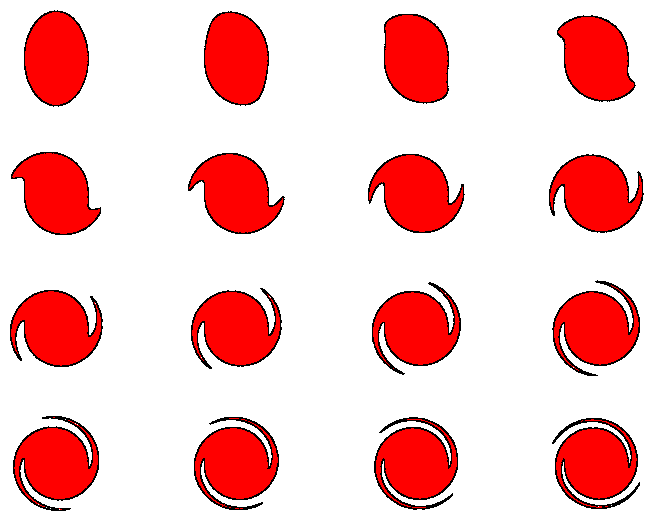
\includegraphics[width=0.6\textwidth]{filament}
\caption{\label{fig:filament} 束团相空间丝化效应示意图\cite{Baartman:2000aa}}
\end{figure}

\subsection{束线元件的球差与色差对束流发射度的影响}
束线上的束流操纵元件,例如螺线管线圈、四极铁等,都或多或少有球差和色差。当束流纵向各切片不在同一个位置经过元件时,元件的球差会对束流各切片有不同的作用;当束流沿纵向有能散时,元件的色差也会导致束流各切片受到作用力不同。如前所述,各切片作用力不同就会导致投影发射度的增长。下式给出了螺线管的色差对束流发射度的影响\cite{Dowell:2010ab}:
\begin{equation}
\varepsilon = \beta\gamma\sigma_x^2\sigma_p\left|\frac{d}{dp}\left(\frac{1}{f_{\text{sol}}}\right)\right|
\end{equation}
代入螺线管线圈焦距公式,就有:
\begin{equation}
\varepsilon = \beta\gamma\sigma_x^2K(\sin KL+KL\cos KL)\frac{\sigma_p}{p}
\end{equation}
其中 $K = B_0/2G_0$,$B_0$ 是螺线管磁感应强度,$G_0$ 是束流中心能量对应的磁钢度。由上式可见,能量较高时,过大的能散也会造成可观的发射度增长。

\section{光阴极微波电子枪束流发射度增长的补偿与抑制}
上一节分析了光阴极微波电子枪(及后续束线)中束流发射度的增长原因,本节就针对各发射度增长机制,介绍相应的补偿或抑制手段。

\subsection{线性发射度增长的补偿}
切片不对齐造成的投影发射度增长一般采用螺线管线圈进行补偿。其基本想法如图 \ref{fig:solcomp} 右图所示:随着束团的运动,束团中各切片由于受力不同而逐渐错开(受力大的切片转动更快),造成发射度增长;在束流传输时加入一个螺线管线圈,相当于引入一个透镜,束团中各切片经过透镜时空间分布不变而动量分布有一个跳变。选择适当的透镜焦距,可以使束团处于聚焦状态。此时受力较小的切片从聚焦状态变回发散状态的速度先慢后快,受力较大的切片从聚焦状态变回发散状态则速度比较均匀。因此在传输一定距离后,受力较小的切片在相空间中后来居上追上之前领先的受力较大的切片,各切片再次在相空间相互重合,这就是线性发射度增长补偿的基本原理\cite{Anderson:2002ab}。
\begin{figure}[htbp]
\centering
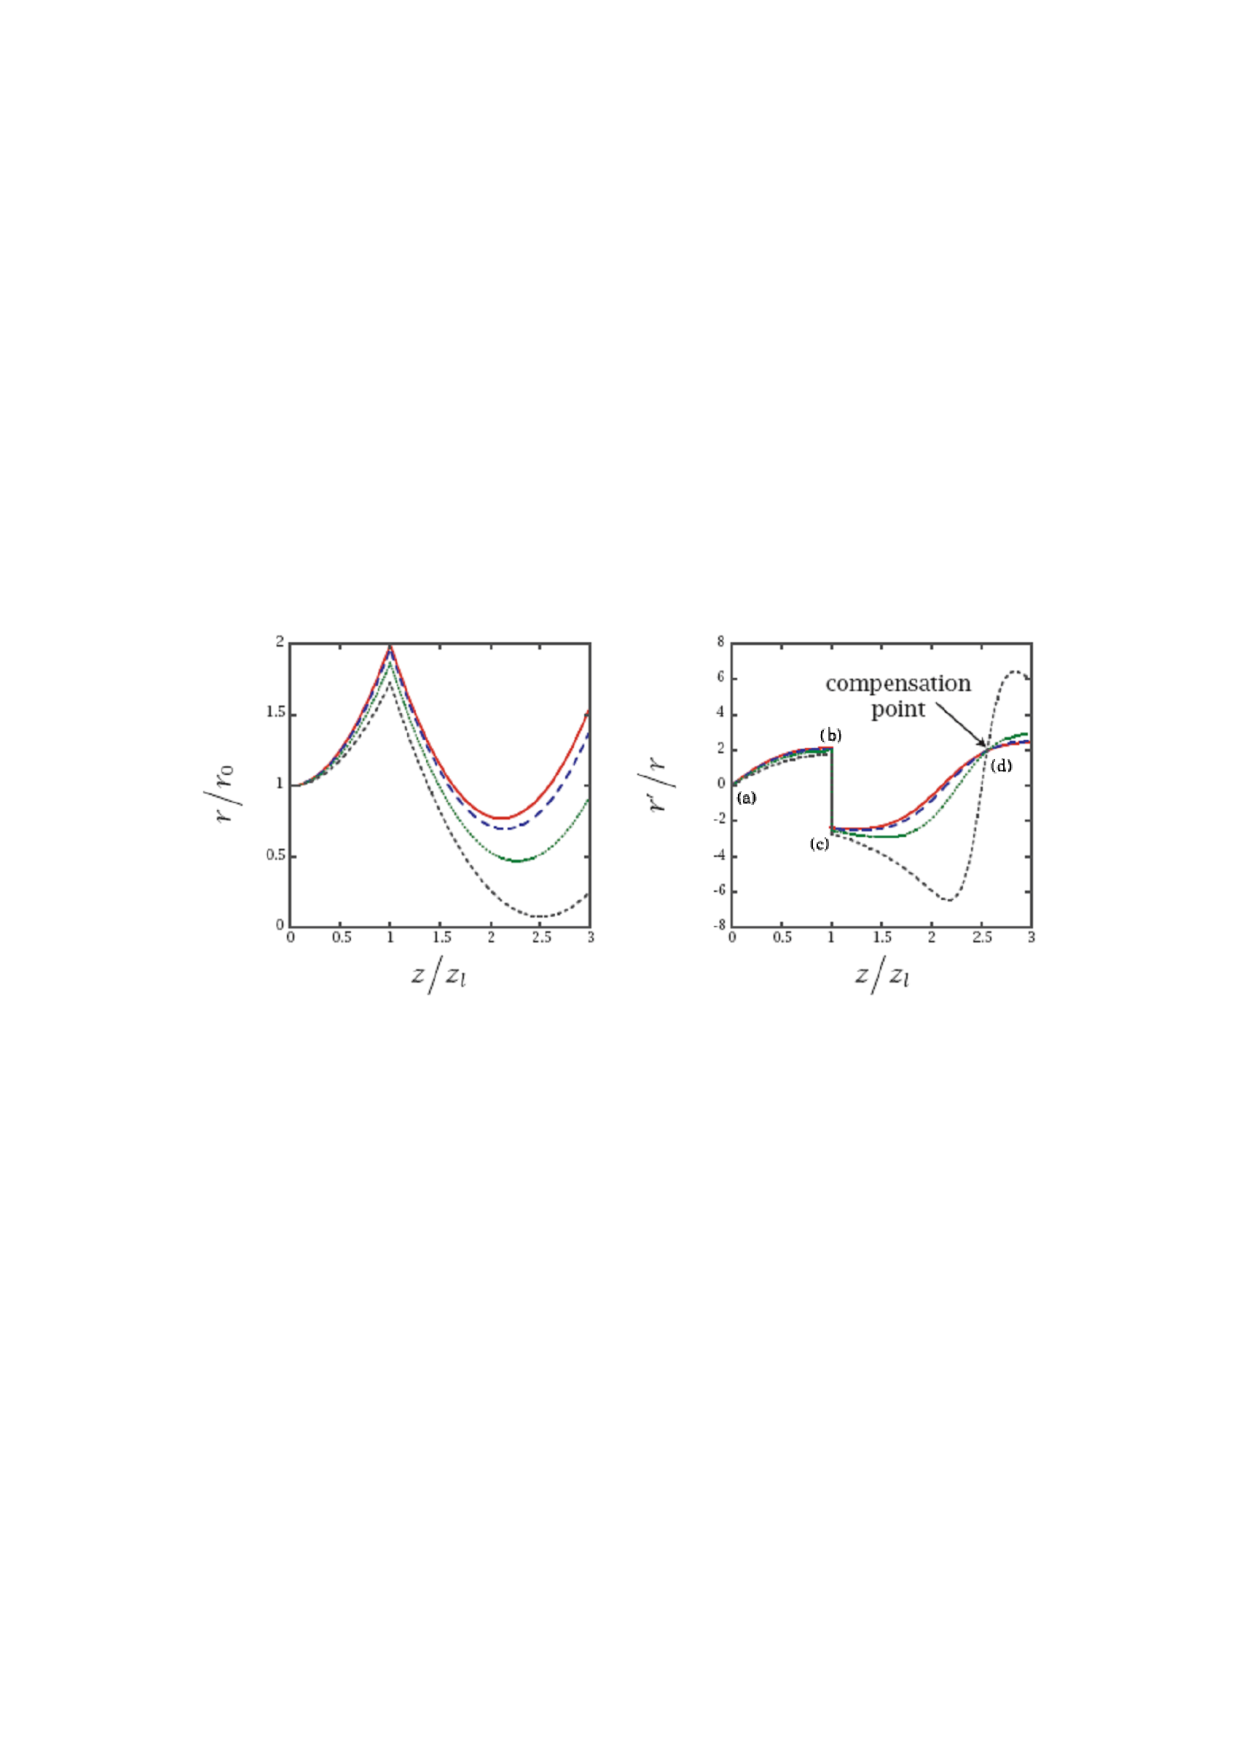
\includegraphics[width=0.9\textwidth]{solcomp}
\caption{\label{fig:solcomp} 螺线管线圈补偿线性发射度增长的原理示意图\cite{Anderson:2002ab}。}
\end{figure}

\subsection{非线性发射度增长的抑制}
对于非线性 RF 作用而言,抑制发射度增长一般采用对称化的电子枪设计以减少结构引入的非线性力;同时可以缩短束流长度,使束流所占微波相位上,微波场强度基本呈线性,以减小纵向高阶分量引入的横向非线性力;人们还提出一种空间叠合型双频电子枪的概念,通过将基模与高阶模重叠在同一个腔体内,达到将 RF 部分相位区间中场强线性化的目标。

对于非线性空间电荷力,目前常采用的方法是设法使束流为 KV 分布(Kapchinskij-Vladimirskij Distribution)\cite{Kapchinskij:1959aa},以从根本上消除非线性空间电荷力。常用的产生 KV 分布束流的方式有:三维激光整形,扁平束发射(pancake regime)和笔形束发射(cigar regime)。

\subsubsection{KV 分布、扁平束与笔形束}
三维 KV 分布即六维椭球面上的均匀分布,实空间体现为三维椭球均匀分布。下面用二维 KV 分布(横向四维椭球面上的均匀分布)为例,给出 KV 分布的形式及其基本性质。二维 KV 分布的形式如下:
\begin{equation}
f(x, y, x^{\prime}, y^{\prime}) = \frac{\lambda}{Q\pi^2\varepsilon_x\varepsilon_y}\delta\left[\left(\frac{x}{\sigma_x}\right)^2+\left(\frac{\sigma_x x^{\prime}-\sigma_x^{\prime} x}{\varepsilon_x}\right)^2+\left(\frac{y}{\sigma_y}\right)^2+\left(\frac{\sigma_x x^{\prime}-\sigma_x^{\prime} x}{\varepsilon_x}\right)^2\right]
\end{equation}
其中 $\lambda$ 为此纵向切片处的线电荷密度,$Q$ 为束团总电荷量。对 $(x^{\prime}, y^{\prime})$ 空间积分,就有:
\begin{equation}
n(x, y) = \frac{\lambda}{Q\pi\sigma_x\sigma_y},\quad (x/\sigma_x)^2+(y/\sigma_y)^2 < 1
\end{equation}
也即实空间中电荷均匀分布在一个椭球(椭圆)内部。KV 分布是唯一使各方向空间电荷力为线性的分布\cite{Kapchinskij:1959aa}。

扁平束即纵横比远小于 1 的束流,在发射过程中,由于其极强的纵向空间电荷力,扁平束流会在很短时间内纵向膨胀成为一个准 KV 分布束团;笔形束与扁平束正相反,它的纵横比远大于 1,是靠其极强的横向空间电荷力,在发射后迅速横向膨胀成为一个准 KV 分布束团。虽然扁平束和笔形束的最终形态都接近 KV 分布,但由于其膨胀过程是个强非线性过程,低的发射度在膨胀时可能会被破坏,所以产生 KV 分布最理想的办法就是用 KV 分布的激光入射直接产生 KV 分布的初始电子束,然而目前的激光技术尚不足以产生精度足够的三维椭球均匀分布的激光脉冲,因此消除非线性空间电荷力的技术依然处于发展中。

\subsubsection{抑制非线性力发射度增长中面临的问题}
非线性 RF 场发射度抑制与非线性空间电荷力发射度抑制之间存在矛盾:为抑制非线性空间电荷力发射度增长,需要将束团尽量拉长;然而拉长后的束团又在射频场中占有相当相位,这就会造成非线性 RF 场发射度的增长;反之亦然,缩短束团长度可以抑制非线性 RF 场发射度的增长,但也会造成初始非线性空间电荷力的增长。两者之间此消彼长。

克服二者的矛盾,可以:1)设法将射频场某相位区间的场强线性化,这也就是双频电子枪的基本想法;2)直接产生较长的 KV 分布的束团;3)提高阴极表面场强,抑制非线性空间电荷力发射度。然而以上三种办法均有自己的缺点:空间叠加型双频电子枪结构复杂,调谐困难;激光的三维整形技术尚不成熟,且由于阴极表面的镜像电荷效应,初始服从 KV 分布的束团若电荷量太大会出现畸变,因此只限于产生低流强的束团;阴极表面场强由电子枪对暗电流/打火等因素的容忍程度限制,不能无限制提高。如何更有效地抑制电子枪(或注入器)中的非线性力发射度增长,依然是一个研究热点。

\section{小结}


%!TEX root = ../main.tex
\chapter{随机缓变粗糙表面光阴极的粗糙度热发射度}
\label{chap:roughness}

为在注入器中产生高亮度的电子束团,需要束团在光阴极表面产生时就具有相当高的品质。因此,光阴极追求尽可能小的热发射度以及尽可能大的量子效率。D. Dowell 利用光电效应的三步模型给出了单光子光电效应光滑金属阴极体发射情形中,量子效率与发射度的公式:
\begin{eqnarray}
\text{QE}(\omega) &\approx& \dfrac{1-R(\omega)}{1+\dfrac{\lambda_{\text{opt}}}{\lambda_{e-e}(\omega)}}\frac{(\hbar\omega-\phi_{\text{eff}})^2}{8\phi_{\text{eff}}(E_F+\phi_{\text{eff}})}\label{eq:QE_d}\\
\varepsilon_{n,x} &=& \sigma_x\sqrt{\dfrac{\hbar\omega-\phi_{\text{eff}}}{3mc^2}}\label{eq:emit_d}
\end{eqnarray}

公式 \ref{eq:QE_d} 与 Cu 阴极的实验结果符合的相当好,但是公式 \ref{eq:emit_d} 却与各实验室的测量值出现了相当大的偏差。若采用 Cu 的文献逸出功 $\phi=4.65\,\text{eV}$,则各实验室的测量值均比公式预测值大 2 倍左右。一般猜测热发射度的增大是由光滑表面的假设失效导致的,也即热发射度中也包含了表面粗糙度的贡献。表面粗糙度对热发射度的贡献分成两种,一种是由于电子发射方向在粗糙表面的离散造成的热发射度,另一种是由阴极表面杂散电场造成的热发射度。对于计算粗糙度热发射度对总体热发射度的贡献,文献中往往采用二维模型或单频三维模型给出大概的量级,半定量地说明粗糙度对热发射度有较大贡献,但却无法和测量值做更精细的比较。因此粗糙度热发射度是否是发射度测量值大于理论值的唯一原因,尚无定论。

本章的目的就是较精确的计算三维粗糙表面粗糙度对热发射度的贡献,为此,需要精确计算激光入射后在粗糙表面产生的出射电子相空间分布。该分布可以利用光阴极的点扩散函数求出。需要注意的是,使用三步模型计算光电发射过程中,本章采取了和 Dowell 相似的假设,即体发射假设,因此本章给出的具体公式仅适用于体发射情形。但是利用点扩散函数来精确计算粗糙度对热发射度贡献的思路与发射模型无关,依然适用于表面发射等更广泛的情形。

\section{\label{s:psf}光阴极的点扩散函数}
当激光入射一个均匀 YAG 屏时,为了预测 YAG 屏上的图像,我们只需要知道激光的横向功率密度分布,以及激光单点入射时屏幕上的图像。后者就是 YAG 屏的点扩散函数(Point Spread Function,PSF)。点扩散函数本质上描述了 YAG 屏对于激光的冲击响应。假设屏幕的点扩散函数为 $f(x, y)$,激光横向功率密度分布为 $I(x, y)$,那么激光入射屏幕时的图像 $D(x, y)$ 就可写成二者的卷积:
\begin{equation}
D(x, y) = I(x, y) * f(x, y)
\label{eq:PSF}
\end{equation}

当我们考虑一个光阴极对入射激光的响应时,也可借鉴类似的概念,唯一的不同在于,光阴极对激光的响应是出射电子的相空间分布,即同时包含空间分布和动量分布;而屏幕对激光的响应是屏幕上的亮度分布,只是空间分布。若我们可以求出光阴极表面任意位置的点扩散函数(不同位置由于起伏可能点扩散函数不同),那么当我们知道入射激光的分布时,就可以直接通过卷积求出光阴极的出射电子相空间分布,从而计算出精确的发射度。下面我们从简单情形考虑,先计算正入射情形下的点扩散函数。

\subsection{正入射情形的光阴极点扩散函数}
为推导光阴极点扩散函数的解析形式,我们采用和 Dowell 相同的假设,即:体发射模型,阴极表面光滑,临界发射(即所有光电子在金属中无散射)。推导中所采用的坐标系统如图 \ref{fig:coor} 所示。

\begin{figure}[htbp]
\centering
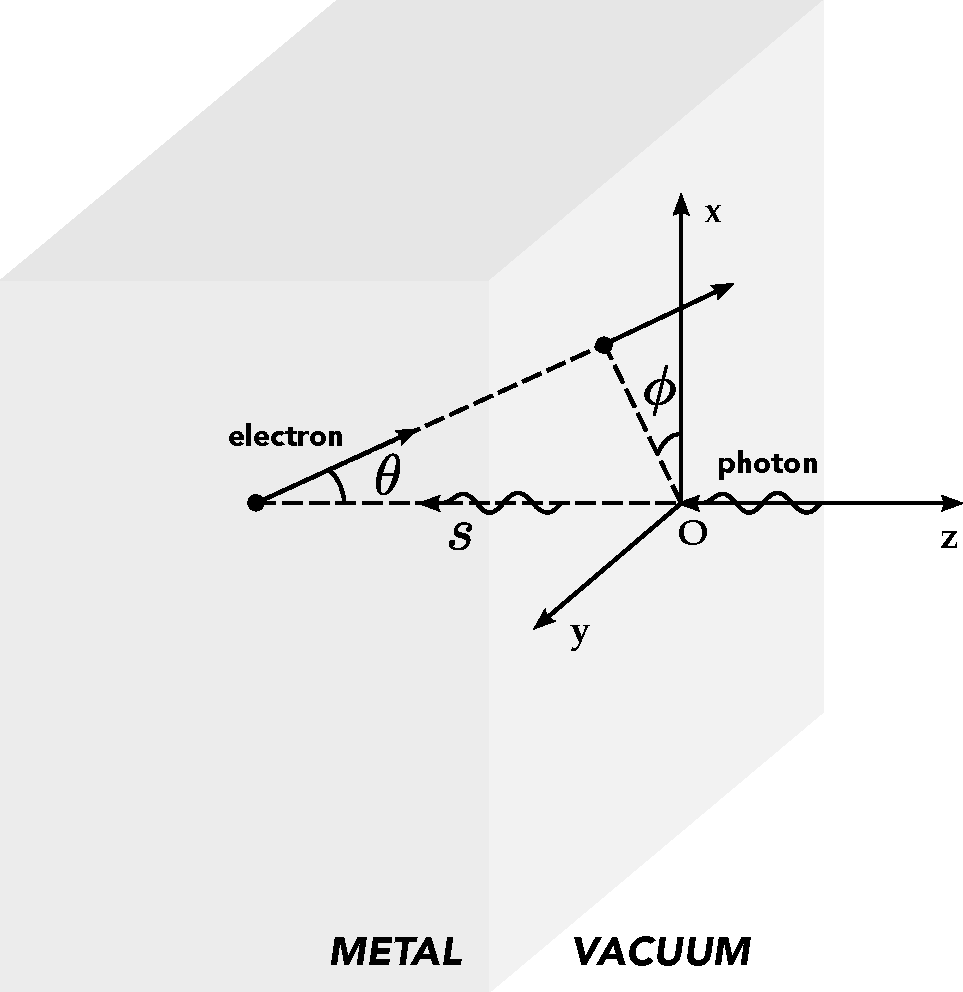
\includegraphics[width=0.5\textwidth]{coor}
\caption{\label{fig:coor} 单点正入射情形下光滑金属阴极体发射示意图,坐标和变量的定义请参见图中标注。}
\end{figure}

采用三步模型,我们可以获得一个正入射的光子入射阴极后,行进距离 $s$ 后被一个能量为 $E$ 的电子所吸收,随后该电子以空间角 $(\theta, \phi)$ 无散射出射并最终逃逸出金属表面成为光电子的概率密度。公式如式 \ref{eq:f} 所示。

\begin{eqnarray}
f(s, \theta, \phi, E, \omega) &=& (1-R)\dfrac{1}{\lambda_{\text{opt}}}\exp\left[-s\left(\dfrac{1}{\lambda_{\text{opt}}} + \dfrac{1}{\bar{\lambda}_{\text{e-e}}}\right)\right]\nonumber\\
&&\cdot\dfrac{H(E_\text{F}-E)H(E+\hbar\omega-E_\text{F})}{\hbar\omega}\dfrac{\sin\theta}{4\pi}
\label{eq:f}
\end{eqnarray}

式 \ref{eq:f} 中的 $H(x)$ 函数是 Heaviside 阶跃函数。为简化形式,令:
\begin{eqnarray}
\frac{1}{\lambda} &=& \frac{1}{\lambda_{\text{opt}}} + \frac{1}{\bar{\lambda}_{\text{e-e}}}\nonumber\\
C &=& \frac{1-R}{\lambda_{\text{opt}}\cdot 4\pi\hbar\omega}\\
p_m &=& \sqrt{2m(E_F+\phi_{\text{eff}})}\nonumber\\
p_M &=& \sqrt{2m(E_F+\hbar\omega)}\nonumber
\label{eq:pm}
\end{eqnarray}
考虑到两组坐标 $(s, \theta, \phi, E, \omega)$ 和 $(x, y, p_x, p_y, p_z)$ 之间的关系:
\begin{eqnarray}
x &=& s\tan\theta\cos\phi\nonumber\\
y &=& s\tan\theta\sin\phi \nonumber\\
p_x &=& \sqrt{2m(E+\hbar\omega)}\sin\theta\cos\phi\\
p_y &=& \sqrt{2m(E+\hbar\omega)}\sin\theta\sin\phi\nonumber\\
p_z &=& \sqrt{2m(E+\hbar\omega)\cos^2\theta - 2m(E_F+\phi_{\text{eff}})}\nonumber
\label{eq:trans}
\end{eqnarray}
我们可以尝试采用雅可比矩阵进行坐标变换。然而不幸的是,上面两组坐标系统并不是一一对应的,因此雅可比行列式为 0,也就是说,我们无法直接通过雅可比矩阵将两个坐标系下的概率分布建立连接。考虑到单点正入射情形时的出射电子相空间分布的轴对称性,采用一个中转坐标系 $(r, p_r, p_z)$ 可以达成连接的目的。

对 $f(s, \theta, \phi, E, \omega)$ 的 $\phi$ 进行积分,可以获得:$f(s,\theta,E;\omega) = 2\pi Ce^{-\frac{s}{\lambda}}\sin\theta$。之后令 $p=\sqrt{2m(E+\hbar\omega)}$,就可以建立起 $(s,\theta,E)$ 与 $(r, p_r, p_z)$ 之间的连接如下:
\begin{eqnarray}
r &=& s\tan\theta\nonumber\\
p_r &=& p\sin\theta\\
p_z &=& \sqrt{p^2-p_r^2-p_m^2}\nonumber
\label{eq:apatrans}
\end{eqnarray}
两坐标系统间的雅可比行列式为:
\begin{eqnarray}
|J| &=& \left|
\renewcommand{\arraystretch}{2.5}
\begin{array}{ccc}
0 & \dfrac{p_r}{m} & \dfrac{p_z}{m} \\
\dfrac{\sqrt{p_z^2+p_m^2}}{p_r} & -\dfrac{r\sqrt{p_z^2+p_m^2}}{p_r^2} & \dfrac{r}{p_r}\dfrac{p_z}{\sqrt{p_z^2+p_m^2}} \\
0 & \dfrac{\sqrt{p_z^2+p_m^2}}{p_r^2+p_z^2+p_m^2} & -\dfrac{p_rp_z}{\sqrt{p_z^2+p_m^2}(p_r^2+p_z^2+p_m^2)}
\end{array} \right|\nonumber\\
&=& \dfrac{1}{m}\cdot\dfrac{p_z}{p_r}
\end{eqnarray}
于是 $dEdsd\theta = |J|drdp_rdp_z$。进而有 $(r, p_r, p_z)$ 坐标系下的点扩散函数:
\begin{eqnarray}
f(r, p_r, p_z)&=&C\exp\left[-\dfrac{\sqrt{p_z^2+p_m^2}}{p_r}\cdot\dfrac{r}{\lambda}\right]\cdot\dfrac{p_z}{\sqrt{p_r^2+p_z^2+p_m^2}}\nonumber\\
&&\cdot H(p_r)H(p_z)H(r)H(p_M^2-p_m^2-p_r^2-p_z^2)
\end{eqnarray}

现在我们要利用电子相空间分布的轴对称性来将 $(r, p_r, p_z)$ 下的点扩散函数变换到 $(x, y, p_x, p_y, p_z)$ 坐标系中。假定 $(x, y, p_x, p_y, p_z)$ 坐标系下的点扩散函数有下面的一般形式:
\begin{equation}
f(x, y, p_x, p_y, p_z) = g(r, p_r, p_z)\delta(xp_y-yp_x)H(xp_x)
\label{eq:apa_general}
\end{equation}
利用积分恒等关系:
\begin{equation}
dp_z\iint_{p_r}^{p_r+dp_r}\!\!\!dp_x\,dp_y\iint_{r}^{r+dr}\!\!\!dx\,dy\,f(x, y, p_x, p_y, p_z) = f(r, p_r, p_z)\,dr\,dp_r\,dp_z
\end{equation}
可获得 $g(r, p_r, p_z)$ 与 $f(r, p_r, p_z)$ 的关系:
\[
g(r, p_r, p_z) = \dfrac{1}{2\pi}f(r, p_r, p_z)
\]
代入 $r = \sqrt{x^2+y^2}$ 和 $p_r = \sqrt{p_x^2+p_y^2}$ 到式 \ref{eq:apa_general},我们就获得了光阴极的正入射点扩散函数,如式 \ref{eq:psf} 所示。

\begin{eqnarray}
f(x, y, p_x, p_y, p_z)&=&C\exp\left[-\dfrac{\sqrt{p_z^2+p_m^2}}{\sqrt{p_x^2+p_y^2}}\cdot\dfrac{\sqrt{x^2+y^2}}{\lambda}\right]\cdot\dfrac{p_z}{\sqrt{p_x^2+p_y^2+p_z^2+p_m^2}}\cdot \delta(xp_y-yp_x)\nonumber\\
&&\cdot H(p_z)H(xp_x)H(p_M^2-p_m^2-p_x^2-p_y^2-p_z^2)
\label{eq:psf}
\end{eqnarray}

利用式 \ref{eq:psf} 所示的点扩散函数,我们可以精确计算任意横向功率密度分布的激光正入射光滑光阴极后的光电子相空间分布。例如,一个横向高斯分布的激光:
\[
I(x, y) = \dfrac{I_0}{2\pi\sigma_x\sigma_y}\cdot\exp\left[-\left(\dfrac{x^2}{2\sigma_x^2}+\dfrac{y^2}{2\sigma_y^2}\right)\right]
\]
所激发的光电子相空间分布 $G(\bm{x},\bm{p})$ 如式 \ref{eq:guass} 所示。
\begin{eqnarray}
G &=& \dfrac{\sqrt{\pi}}{2}\dfrac{1}{\sqrt{\dfrac{p_x^2}{2\sigma_x^2}+\dfrac{p_y^2}{2\sigma_y^2}}}\exp\left[-\dfrac{x^2}{2\sigma_x^2}-\dfrac{y^2}{2\sigma_y^2}+T^2\right]\cdot\text{erfc}(T)\nonumber\\
T &=& \dfrac{-\dfrac{xp_x}{2\sigma_x^2}-\dfrac{yp_y}{2\sigma_y^2}+\dfrac{\sqrt{p_z^2+p_m^2}}{2\lambda}}{\sqrt{\dfrac{p_x^2}{2\sigma_x^2}+\dfrac{p_y^2}{2\sigma_y^2}}}
\label{eq:guass}
\end{eqnarray}

\subsection{\label{ss:dowell}对 Dowell 发射度公式的修正}
统计意义下的发射度定义如下:
\begin{equation}
\varepsilon_{D,x}^2 = \langle x^2\rangle_D\langle p_x^2\rangle_D-\langle xp_x\rangle_D^2
\label{eq:emit_def}
\end{equation}
式 \ref{eq:emit_def} 中的符号 D 代表电子相空间分布。在 Dowell 发射度公式的推导中,$\langle xp_x\rangle$ 所代表的交叉项被忽略掉了,理由是假设电子动量分布与光子入射位置相互独立。Dowell 同时假定了出射光电子的横向空间分布与入射激光的横向分布相同。若这些假设成立,则统计意义的发射度计算就可以简化为 $\varepsilon_{x} = \sqrt{\langle x^2\rangle\langle p_x^2\rangle}=\sigma_x\sqrt{\langle p_x^2\rangle}$,因此 $\varepsilon_{x,n} = \sigma_x\cdot\Delta_x$,其中 $\Delta_x$ 被称做归一化散角(有时也称为归一化热发射度),定义为 $\sqrt{\langle p_x^2\rangle}/mc$。利用我们前面推导的点扩散函数,通过计算式 \ref{eq:emit_def} 中的各统计项,可以检验 Dowell 发射度公式的精确程度。

假设我们有一个形式为 $v(x,y,p_x,p_y,p_z)$ 的变量 $v$,为了计算 $v$ 在概率密度分布 $D=I*f$ 下的期望,我们有式 \ref{eq:stat} 中所展示的规律:
\begin{equation}
\langle v \rangle_{D} = \langle v\rangle_{I * f} = \langle v(x_I+x_f, y_I+y_f, p_x, p_y, p_z)\rangle_{I\cdot f}
\label{eq:stat}
\end{equation}
式 \ref{eq:stat} 中有下标的 $x$ 或 $y$ 代表它们仅在下标所示的分布中是变量,而在其他分布中是常数。例如当计算 $\langle x_I\rangle_{f}$ 时 $x_I$ 是个常数,而当计算 $\langle x_I\rangle_{I}$ 时则是变量。 同时约定 $\langle\cdots\rangle_{I\cdot f}$ 代表求复合平均 $\langle\langle\cdots\rangle_{I}\rangle_{f}$ 或者 $\langle\langle\cdots\rangle_{f}\rangle_{I}$。由于交换内外括号的下标并不会改变统计结果,我们可以将复合平均符号写做 $\langle\cdots\rangle_{I\cdot f}$。

经过代数计算,最终可获得:
\begin{eqnarray}
\varepsilon_{D, x}^2 &=& \langle x^2\rangle_I\langle p_x^2\rangle_f+\varepsilon_f^2
\label{eq:emit_acc}
\end{eqnarray}
其中 $\varepsilon_f^2$ 代表单点入射发射度,即 $\langle x^2\rangle_f\langle p_x^2\rangle_f-\langle xp_x\rangle_f^2$。式 \ref{eq:emit_acc} 右侧第一项就是 Dowell 给出的发射度公式,所以第二项 $\varepsilon_f$ 就是 Dowell 发射度公式的误差。当 $\hbar\omega$ 接近 $\phi_{\text{eff}}$ 时(也即临界发射,这也是一般光阴极采用的工作状态)。下面我们尝试计算 $\varepsilon_f$。至少有两种方式计算单点热发射度,即 1)直接使用式 \ref{eq:psf} 和 2)采用原始的概率密度公式 \ref{eq:f}。下面使用对人类更友好的第二种方式进行计算。

简化起见,令 $p = \sqrt{2m(E+\hbar\omega)}$ 以及 $\cos\theta_M=p_m/p_M$,也令 $\Delta=p_M-p_m$ 以及 $\delta=(p_M-p_m)/p_m$。应用式 \ref{eq:f},我们有:
\begin{eqnarray*}
\langle x^2\rangle_f &=& \dfrac{\int_{p_m}^{p_M} pdp\int_0^{\infty} ds\int_0^{2\pi}d\phi\int_0^{\theta_M}d\theta (s\tan\theta\cos\phi)^2e^{-\frac{s}{\lambda}}\sin\theta}{\int_{p_m}^{p_M} pdp\int_0^{\infty} ds\int_0^{2\pi}d\phi\int_0^{\theta_M}d\theta e^{-\frac{s}{\lambda}}\sin\theta}\\
&=& \dfrac{\int_{p_m}^{p_M} pdp\int_0^{\infty} s^2e^{-\frac{s}{\lambda}}ds\int_0^{2\pi}\cos^2\phi d\phi\int_0^{\theta_M}\tan^2\theta\sin\theta d\theta}{\int_{p_m}^{p_M} pdp\int_0^{\infty} e^{-\frac{s}{\lambda}}ds\int_0^{2\pi}d\phi\int_0^{\theta_M}\sin\theta d\theta}\\
&=& \dfrac{\int_{p_m}^{p_M}pdp\cdot\lambda^3\Gamma(3)\cdot\pi\cdot(p/p_m+p_m/p-2)}{\int_{p_m}^{p_M}pdp\cdot\lambda\Gamma(1)\cdot2\pi\cdot(1-p_m/p)}\\
&=& \frac{\lambda^2}{p_m}\cdot\dfrac{\Delta^3/3}{\Delta^2/2} = \frac{2}{3}\lambda^2\delta
\end{eqnarray*}

\begin{eqnarray*}
\langle p_x^2\rangle_f &=& \dfrac{\int_{p_m}^{p_M} pdp\int_0^{\infty} ds\int_0^{2\pi}d\phi\int_0^{\theta_M}d\theta (p\sin\theta\cos\phi)^2e^{-\frac{s}{\lambda}}\sin\theta}{\int_{p_m}^{p_M} pdp\int_0^{\infty} ds\int_0^{2\pi}d\phi\int_0^{\theta_M}d\theta e^{-\frac{s}{\lambda}}\sin\theta}\\
&=& \dfrac{\int_{p_m}^{p_M} p^3dp\int_0^{\infty} e^{-\frac{s}{\lambda}}ds\int_0^{2\pi}\cos^2\phi d\phi\int_0^{\theta_M}\sin^3\theta d\theta}{\int_{p_m}^{p_M} pdp\int_0^{\infty} e^{-\frac{s}{\lambda}}ds\int_0^{2\pi}d\phi\int_0^{\theta_M}\sin\theta d\theta}\\
&=& \dfrac{\int_{p_m}^{p_M}p^3dp\cdot\lambda\Gamma(1)\cdot\pi\cdot(2/3-p_m/p+1/3\cdot p_m^3/p^3)}{\int_{p_m}^{p_M}pdp\cdot\lambda\Gamma(1)\cdot2\pi\cdot(1-p_m/p)}\\
&=& \frac{1}{2}\cdot\dfrac{\Delta^4/6+p_m\cdot\Delta^3/3}{\Delta^2/2} = \frac{1}{6}\Delta(\Delta+2p_m)
\end{eqnarray*}

\begin{eqnarray*}
\langle xp_x\rangle_f &=& \dfrac{\int_{p_m}^{p_M} pdp\int_0^{\infty} ds\int_0^{2\pi}d\phi\int_0^{\theta_M}d\theta (sp\tan\theta\sin\theta\cos^2\phi)e^{-\frac{s}{\lambda}}\sin\theta}{\int_{p_m}^{p_M} pdp\int_0^{\infty} ds\int_0^{2\pi}d\phi\int_0^{\theta_M}d\theta e^{-\frac{s}{\lambda}}\sin\theta}\\
&=& \dfrac{\int_{p_m}^{p_M} p^2dp\int_0^{\infty} se^{-\frac{s}{\lambda}}ds\int_0^{2\pi}\cos^2\phi d\phi\int_0^{\theta_M}\tan\theta\sin^2\theta d\theta}{\int_{p_m}^{p_M} pdp\int_0^{\infty} e^{-\frac{s}{\lambda}}ds\int_0^{2\pi}d\phi\int_0^{\theta_M}\sin\theta d\theta}\\
&=& \dfrac{\int_{p_m}^{p_M}p^2dp\cdot\lambda^2\Gamma(2)\cdot\pi\cdot(-1/2-\ln(p_m/p)+1/2\cdot p_m^2/p^2)}{\int_{p_m}^{p_M}pdp\cdot\lambda\Gamma(1)\cdot2\pi\cdot(1-p_m/p)}\\
&=& \frac{\lambda}{2}\cdot\dfrac{\frac{1}{3}p_M^3\ln(p_M/p_m)-\frac{1}{9}(p_M^3-p_m^3)-\frac{1}{6}\Delta^2(p_M+2p_m)}{\Delta^2/2}\\
&=& \frac{1}{3}\lambda \Delta\left(1+\frac{1}{4}\delta+O(\delta^2)\right)\approx\frac{1}{3}\lambda \Delta
\end{eqnarray*}

把上面的计算结果带回统计意义发射度公式,就有:
\begin{eqnarray*}
\varepsilon_f &=& \sqrt{\langle x^2\rangle_f\langle p_x^2\rangle_f-\langle xp_x\rangle_f^2} \approx \frac{1}{3}\lambda\sqrt{\delta\cdot\Delta(\Delta+2p_m)-\Delta^2}\\
&=& \frac{1}{3}\lambda\sqrt{\delta\cdot\Delta^2+2\Delta^2-\Delta^2} = \frac{1}{3}\lambda\sqrt{\Delta^2\cdot(1+\delta)}\\
&\approx& \frac{1}{3}\lambda\Delta = \dfrac{1}{3}\lambda(p_M-p_m)
\end{eqnarray*}
也即 $\varepsilon_f$ 具有下面的近似形式:
\[
\varepsilon_f \approx \dfrac{1}{3}\lambda(p_M-p_m)
\]
其中 $p_M,p_m$ 和 $\lambda$ 与 式 \ref{eq:pm} 中的定义相同。而 $\langle p_x^2\rangle_f$ 可以写成:
\[
\langle p_x^2\rangle_f = \dfrac{1}{6}(p_M^2-p_m^2)
\]
取一阶近似,则修正后的发射度公式的近似形式就如下式所示:
\begin{equation}
\varepsilon_{D,x}^2 \approx \varepsilon_{\text{Dowell}}^2\left[1+\left(\dfrac{\lambda}{\sigma_x}\right)^2\cdot\dfrac{\delta}{3}\right]
\label{eq:emit_de}
\end{equation}
其中 $\delta = (p_M-p_m)/p_m$。代入表 \ref{tab:exp} 中所示的一组典型的实验参数,就有:
\[
\varepsilon_{D,x}^2 = \varepsilon_{\text{Dowell}}^2\left[1+\left(\dfrac{0.40\,\text{nm}}{\sigma_x}\right)^2\right]
\]

由于 $\sigma_x$ 的典型值在 100\,$\mu$m 量级,从上式可以看出,绝大多数情形下,Dowell 公式足够精确,在发射度计算中可以忽略动量分布与入射位置间的关系。

\begin{table}[htbp]
\caption{\label{tab:exp}
一组典型的光阴极物理参数。}
\centering
\begin{tabular}{llll}
\toprule
参数 & 值 & 单位 & 描述 \\
\midrule
$E_F$ & 7.0 & eV & Cu 的费米能级 \\
$\hbar\omega$ & 4.66 & eV & 光子能量 \\
$\phi_w$ & 4.31 & eV & Cu 的逸出功 \\
$E_{\text{rf}}$ & 50.0 & MV/m & 阴极表面电场强度 \\
$\lambda_{\text{opt}}$ & 12.58 & nm & Cu 中光子的平均自由程 \\
$\bar{\lambda}_{\text{e-e}}$ & 6.13 & nm & Cu 中电子的平均自由程 \\
\bottomrule
\end{tabular}
\end{table}

\subsection{\label{ss:approx}光电子相空间分布的近似形式}
从小节 \ref{ss:dowell} 中证明了一般情况下忽略电子动量分布与光子入射位置之间的关系是合理的,事实上这个结论可以从点扩散函数的观点直接得到。

考虑阴极表面点 \textbf{P}$(x_0, y_0)$ 附近的光电子相空间分布。利用式 \ref{eq:psf} 中给出的点扩散函数,容易证明点扩散函数的 rms 半径在亚纳米量级,且点扩散函数的幅度在 rms 半径外的区域迅速衰减到 0。因此我们定义以 \textbf{P} 点为中心 rms 半径为半径的圆形区域为有效区域。由于有效区域非常小,可以假设激光功率密度在 \textbf{P} 点的有效区域内基本为常数。同时对于有效区域外的被照射表面,其发射电子对点 \textbf{P} 处光电子相空间的贡献基本可以忽略。根据以上分析,点 \textbf{P} 处的光电子相空间分布可以近似如下:
\begin{eqnarray}
D\big|_{\textbf{P}} &=& I(x,y)*f(x,y,p_x,p_y,p_z)\big|_{x=x_0,y=y_0}\nonumber\\
&\approx& I(x_0,y_0)*f(x,y,p_x,p_y,p_z)\big|_{(x, y)\text{ in effective area}}\nonumber\\
&\approx& I(x_0,y_0)*f(x,y,p_x,p_y,p_z)\big|_{(x, y)\text{ in entire area}}\nonumber\\
&=& I(x_0,y_0)\cdot\iint dxdyf(x,y,p_x,p_y,p_z)\nonumber\\
&=& I(x_0,y_0)f_p(p_x,p_y,p_z)
\label{eq:approx}
\end{eqnarray}
上式就验证了前面的结论。

式 \ref{eq:approx} 中的函数 $f_p(p_x, p_y, p_z)$ 是动量点扩散函数,它描述了单点入射情形下的光电子动量空间分布。正如式 \ref{eq:approx} 所示,$f_p$ 就是 $f$ 对整个实空间 $(x, y)$ 的积分,因此可以计算得到动量点扩散函数的形式如下:
\begin{eqnarray}
f_p(p_x,p_y,p_z) &=& \dfrac{C_p p_z}{\sqrt{{p_z}^2+p_m^2}\cdot\sqrt{{p_x}^2+{p_y}^2+{p_z}^2+{p_m}^2}}\nonumber\\
&&\cdot H(p_z)H(p_M^2-p_m^2-p_x^2-p_y^2-p_z^2)
\label{eq:ppsf}
\end{eqnarray}
其中 $C_p$ 满足:
\[
C_p = \dfrac{1-R}{1+\dfrac{\lambda_{\text{opt}}}{\lambda_{e-e}}}\cdot\dfrac{1}{4\pi m\hbar\omega}
\]
近似形式的光电子分布函数将会在接下来的一般表面粗糙度热发射度计算中起到关键作用。

\section{\label{s:ana}随机缓变粗糙表面光阴极的粗糙度热发射度}
采用点扩散函数的独特好处在于,它可以处理真实场景下几乎任意表面形态的光阴极的热发射度。这里强调真实场景,是因为真实的光阴极通常是经过精细加工与打磨的,其表面在宏观上非常接近一个平面;但是从微观上看,加工过程中的车铣会在其表面留下较规则的条纹,其横向尺度一般在十几微米,起伏在百纳米级别,而打磨时会在阴极表面留下非常细小的起伏,其横向和纵向尺度一般在百纳米到纳米量级。尽管真实阴极表面会存在这些不均匀的形态,但其总体上依然是一个相当平滑的平面,我们称这种表面为随机缓变粗糙表面。

\subsection{缓变粗糙表面}
图 \ref{fig:rough} 展示了白光干涉仪下的一块真实阴极的表面形态,其局部的三维视图见 \ref{fig:rough-3D}。
\begin{figure}[htbp]
\centering
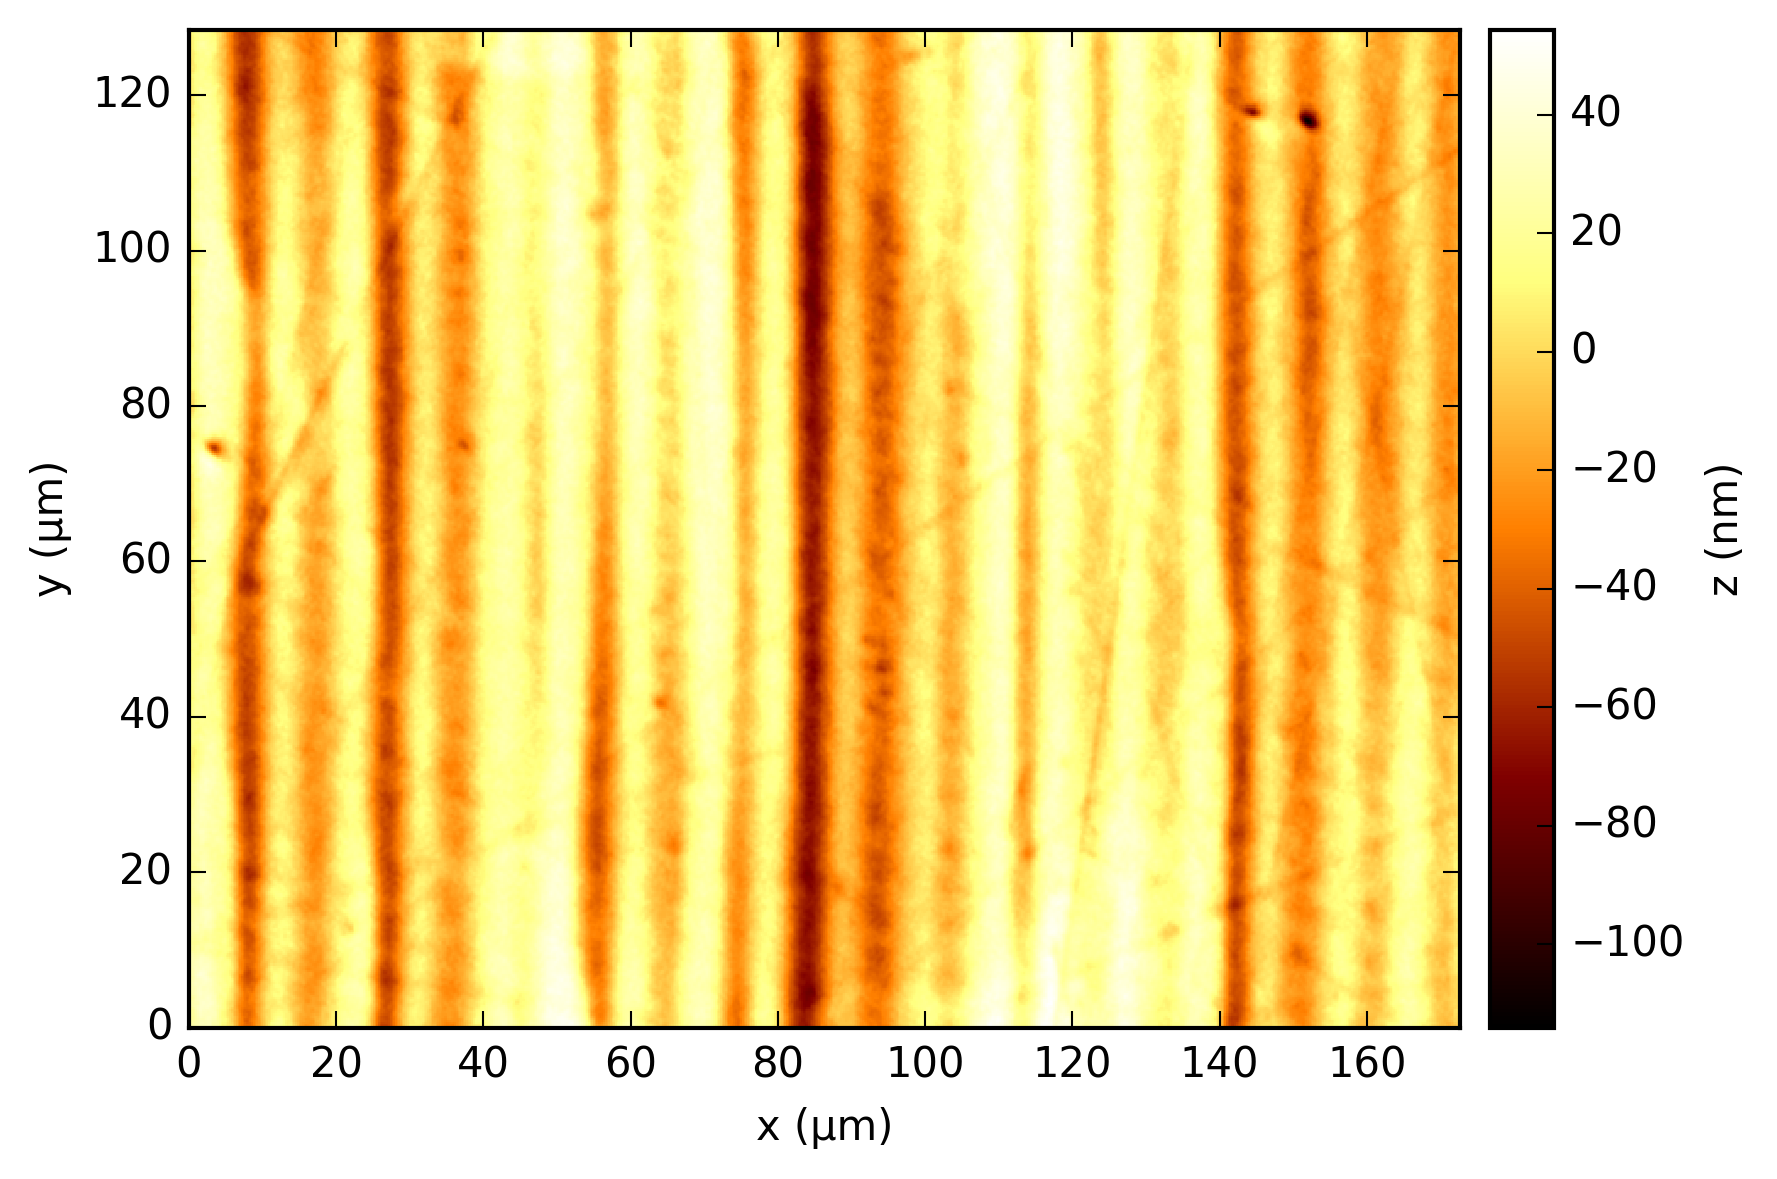
\includegraphics[width=0.45\textwidth]{surface-all}
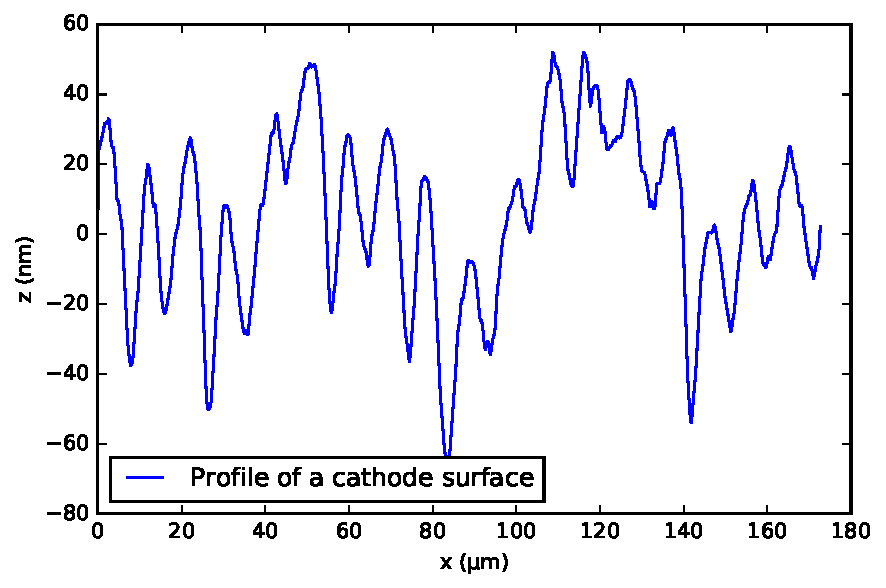
\includegraphics[width=0.45\textwidth]{profile}
\caption{\label{fig:rough} 白光干涉仪下一块真实阴极的表面形态。左图:测量表面俯视图;右图:某截面的轮廓,注意横纵坐标的单位不同。}
\end{figure}

人们通常使用振幅 $a$ 与空间周期 $\lambda$(或空间波数 $k$)来描述粗糙度的某个特定空间频率的分量。如前所述,一块经过抛光的阴极上通常存在两种粗糙度,即宏观粗糙度 $r_M$ 与微观粗糙度 $r_m$。这两种粗糙度的典型参数见表 \ref{tab:rough}。

\begin{figure}[htbp]
\centering
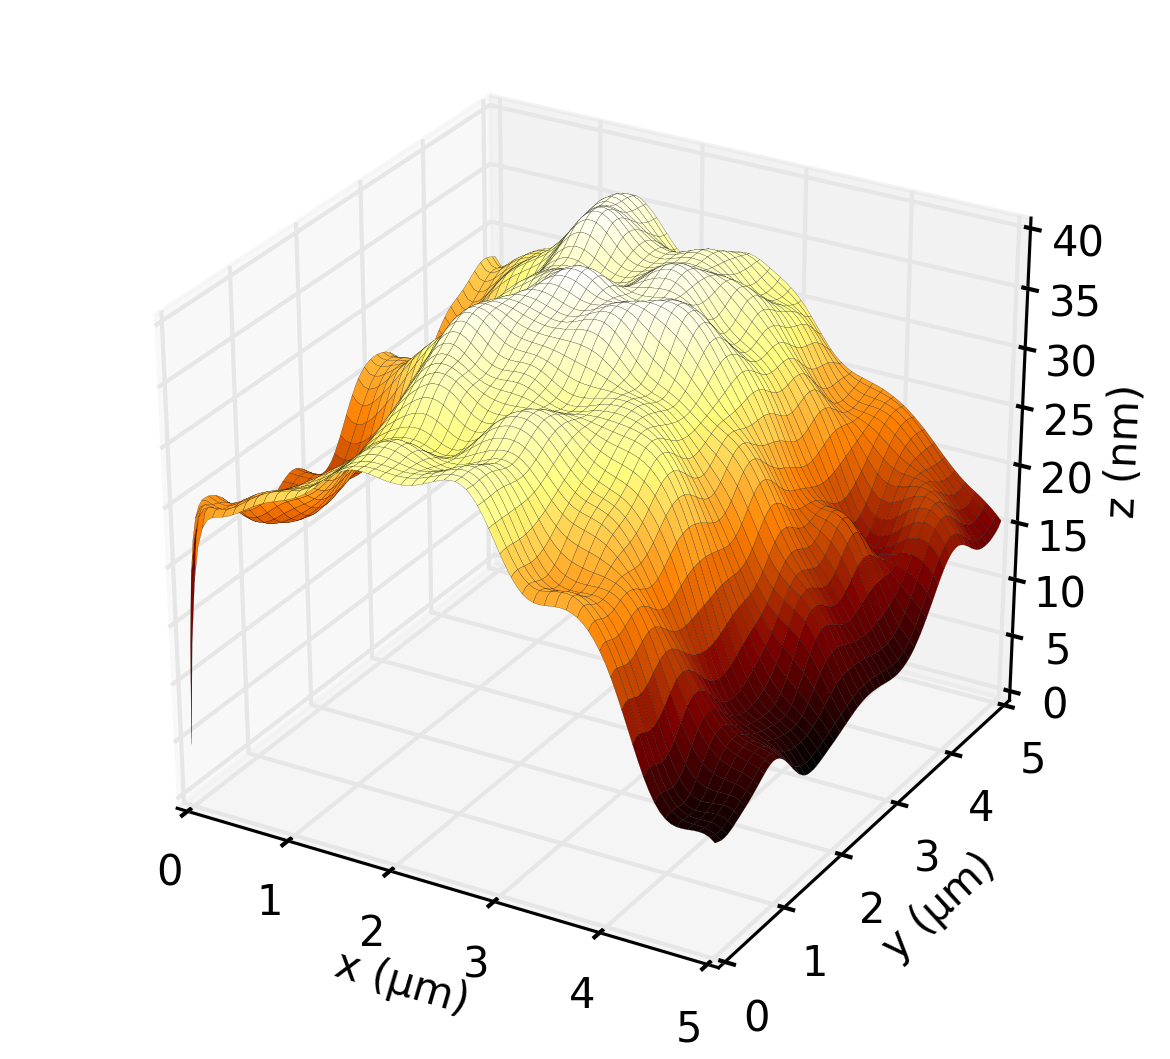
\includegraphics[width=0.6\textwidth]{surface}
\caption{\label{fig:rough-3D} 白光干涉仪下一块真实阴极的局部形态。注意横纵坐标的单位不同。}
\end{figure}

\begin{table}[htbp]
\caption{\label{tab:rough}
粗糙度参数的典型值。}
\centering
\begin{tabular}{llll}
\toprule
参数 & 值 & 单位 & 描述 \\
\midrule
$a_m$ & 4 & nm & 微观粗糙度典型振幅 \\
$\lambda_m$ & 200 & nm & 微观粗糙度典型空间周期 \\
$a_M$ & 100 & nm & 宏观粗糙度典型振幅 \\
$\lambda_M$ & 16 & $\mu$m & 宏观粗糙度典型空间周期 \\
\bottomrule
\end{tabular}
\end{table}

缓变粗糙表面很难严格界定,因为不同情形下对缓变和粗糙的定义不同。但在光阴极领域,我们可以认为缓变粗糙表面有下面特征:其大部分空间分量的梯度都远小于 1。根据这个特点,定义某方向 $x$ 的缓变粗糙表面为满足下面条件的表面:
\begin{equation}
\text{rms}(R)\cdot\text{rms}(k_x) \ll 1
\label{eq:def_gus}
\end{equation}
其中 $k_x$ 是 $x$ 方向的空间波数, $R$ 是待考虑表面的振幅。 

这个定义其实是保证对于所有 $k \le k_{\max}$,$k\cdot R(x, y) \ll 1$。这里 $k_{\max}$ 我们所考虑的最大空间波数,因为对于 $k > k_{\max}$ 的空间分量,其振幅已经小到可以在计算粗糙度热发射度时忽略不计。我们以图 \ref{fig:conf} 所示的真实阴极表面为例,其空间频谱见图 \ref{fig:spec}。对该粗糙阴极表面计算得到各统计值如下:$\text{rms}(k_x)=3.45\,\mu\text{m}^{-1}, \text{rms}(R)=22.65\,\text{nm}$,因此 $\text{rms}(R)\cdot\text{rms}(k_x) = 0.08 \ll 1$。从频谱的强度分布可以看出,我们所关心的最大波数 $k_{x, \max}\sim 4\,\mu\text{m}^{-1}$(因为大部分的空间分量的能量都集中在这个区域内)。对于这个表面,容易看出 $\text{rms}(k_x)\sim k_{x, \max}$ 并且 $R(x, y)\sim\text{rms}(R)$,因此我们的定义式 \ref{eq:def_gus} 可以保证对于所有 $k \le k_{\max}$ 都有 $k\cdot R(x, y) \ll 1$。

本章接下来所有的讨论和推导都仅限于这种缓变粗糙表面。
%Paper~[5] assumed the surface morphology obey the form:
%\[ 
%R(x, y)=h\cos(kx)\cos(ky)
%\]which described a quasi-monochrome roughness, to derive the analytical formation of the roughness emittance. The result of paper~[5] showed that: $\varepsilon_{\text{roughness}}\propto \xi$, $\xi=hk$.

\subsection{\label{ss:gmpsf}推广的动量点扩散函数}

\begin{figure}[htbp]
\centering
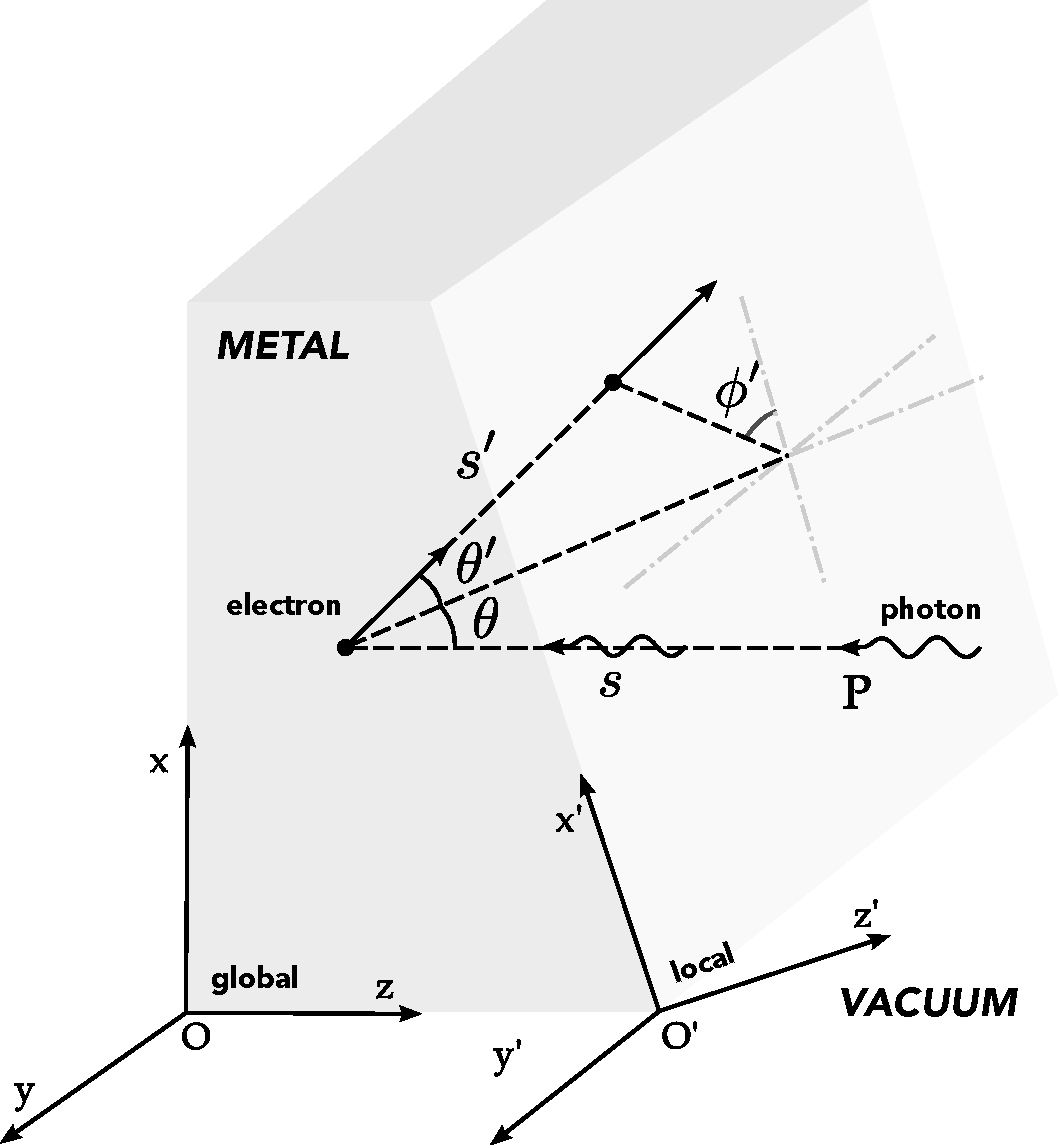
\includegraphics[width=0.5\textwidth]{coor2}
\caption{\label{fig:coor_m} 粗糙阴极表面某局部的体发射示意图。坐标系统和变量定义如图中标注所示。光滑和粗糙阴极的主要区别在于,对于粗糙阴极而言,激光基本上在表面任何一点都是(相对于该处法向)斜入射的。如图所示,一个光子以 $\theta$ 的入射角入射,在行进 $s$ 距离后,光子被一个电子吸收,随后电子向粗糙表面运动并成功逃逸处金属表面成为光电子。很明显斜入射时光电子发射的中心点不再是光子入射点 \textbf{P},而是距离点 \textbf{P} 有一个小的偏移。}
\end{figure}

当一束激光正入射一个表面形态函数为 $R(x, y)$ 的粗糙表面时,我们跟踪其中一个光子来看看中间的物理过程。假定该光子从阴极表面 \textbf{P}$(x_0, y_0)$ 点入射,由于点 \textbf{P} 的法向相对于全局坐标系的 z 轴存在一个夹角,光电发射过程除了发射中心不再是入射点外,其他几乎与光滑平面阴极的情形没有区别。

采用点扩散函数的观点来考虑上面的进程,我们可以采用和小节 \ref{ss:approx} 类似的想法。点 \textbf{P} 的邻域 $\Delta$ 可以看成一个法向相对于 $z$ 轴成一个夹角 $\theta$ 的平面,且激光功率密度在有效区域内近似常量 $I(x_0, y_0)$。为获得全局坐标系 $S$ 下的光电子相空间分布,可以首先获取局部坐标系 $S^{\prime}$(法向与全局坐标系 $z$ 轴成 $\theta$ 的夹角)下的光电子相空间分布 $D^{\prime}$,随后旋转 $D^{\prime}$ 到全局坐标系,进而获得 $D$。

为实现上面的想法,有必要将原始的正入射动量点扩散函数推广到一般入射情形。通过一定的计算,得到推广的动量点扩散函数如式 \ref{eq:g-ppsf} 所示。

\begin{eqnarray}
f_p(p_x,p_y,p_z) &=& \dfrac{C_p(\theta)p_z}{\sqrt{p_z^2+p_m^2}\cdot\sqrt{p_x^2+p_y^2+p_z^2+p_m^2}}\label{eq:g-ppsf}\\
C_p(\theta) &=& \dfrac{1-R(\theta)}{1+\dfrac{\lambda_{\text{opt}}}{\lambda_{e-e}}\cos\theta}\cdot\dfrac{1}{4\pi m\hbar\omega}\nonumber
\end{eqnarray}
为了使公式清晰我们省略了 Heaviside 阶跃函数。结合式 \ref{eq:approx} 和 \ref{eq:g-ppsf},获得局部坐标系下的光电子相空间分布:
\begin{equation}
D^{\prime}(x, y, p_x, p_y, p_z) = I(x_0,y_0)\cos\theta f_p(p_x, p_y, p_z)
\label{eq:l-dist}
\end{equation}

下一步是利用局部坐标系到全局坐标系的旋转矩阵将局部坐标系下光电子相空间分布变换到全局坐标系下。
将式 \ref{eq:g-ppsf} 代入式 \ref{eq:l-dist} 可以获得全局坐标系下分布的形式:
\begin{equation}
D^{\prime}= I(x_0,y_0)\cos\theta \dfrac{Cp_z^{\prime}}{\sqrt{{p_z^{\prime}}^2+p_m^2}\cdot\sqrt{{p_x^{\prime}}^2+{p_y^{\prime}}^2+{p_z^{\prime}}^2+p_m^2}}
\label{eq:apc_l2d}
\end{equation}
设局部与全局坐标系之间的变换矩阵为:
\begin{equation}
\mathbf{D}=\left(
\begin{array}{c}
\mathbf{m}\\
\mathbf{n}\\
\mathbf{k}
\end{array} \right)
\end{equation}
那么:
\begin{equation}
\mathbf{D}\cdot\left(
\begin{array}{c}
p_x\\
p_y\\
p_z
\end{array} \right)=\left(
\begin{array}{c}
p_x^{\prime}\\
p_y^{\prime}\\
p_z^{\prime}
\end{array} \right)
\label{eq:apc_trans}
\end{equation}
我们未指定 $S^{\prime}$ 的具体朝向,所以基向量 $\bm{m}$ 和 $\bm{n}$ 可以随意选择(当然要保证与 $\bm{k}$ 正交)。$\bm{k}$ 是点 \textbf{P} 的法向量,所以其满足:
\begin{equation}
{\mathbf k} = \left(\dfrac{-\partial_xR}{\sqrt{1+\partial_x^2R+\partial_y^2R}},\dfrac{-\partial_yR}{\sqrt{1+\partial_x^2R+\partial_y^2R}},\dfrac{1}{\sqrt{1+\partial_x^2R+\partial_y^2R}}\right)
\label{eq:apc_k}
\end{equation}
将式 \ref{eq:apc_k} 代入式 \ref{eq:apc_trans},就可以得到 $(p_x^{\prime}, p_y^{\prime}, p_z^{\prime})$ 与 $(p_x, p_y, p_z)$ 之间的关系。在式 \ref{eq:apc_l2d} 中将所有项中的 $p^{\prime}$ 替换为 $p$,再考虑到局部坐标系中相空间分布的轴对称性,通过一定计算最终得到全局坐标系下的光电子相空间分布为式 \ref{eq:g-dist}。

事实上,我们在计算粗糙度热发射度时并不需要 \ref{eq:g-dist} 的具体形式,而是可以直接使用式 \ref{eq:l-dist} 来计算点 \textbf{P}$(x_0, y_0)$ 的邻域 $\Delta$ 中在局部坐标系下的统计项,然后使用旋转矩阵去计算全局坐标系下的各统计项。

现在全部准备工作都已做完,可以开始计算粗糙度热发射度了。简单起见,当推导 2D 和 3D 随机表面的粗糙度热发射度时,我们会忽略掉发射权重 $W(\theta)$(定义为 $W(\theta)=\cos\theta\cdot C_p(\theta)$,发射权重其实就是相对量子效率)和入射角度 $\theta$ 之间的关系,理由会在节 \ref{s:num} 中给出。

\begin{eqnarray}
&&D = I(x,y)\cdot\dfrac{\cos\theta\cdot C_p(\theta)(Ap_x+Bp_y+Cp_z)}{\sqrt{(Ap_x+Bp_y+Cp_z)^2+p_m^2}\cdot\sqrt{p_x^2+p_y^2+p_z^2+p_m^2}}\cdot H(p_z)H(p_M^2-p_m^2-p_x^2-p_y^2-p_z^2)\label{eq:g-dist}\nonumber\\
&&(A, B, C) = \left(\dfrac{-\partial_xR}{\sqrt{1+\partial_x^2R+\partial_y^2R}},\dfrac{-\partial_yR}{\sqrt{1+\partial_x^2R+\partial_y^2R}},\dfrac{1}{\sqrt{1+\partial_x^2R+\partial_y^2R}}\right)
\end{eqnarray}

\subsection{\label{ss:2d}2D 正弦表面}
首先我们考虑一个简单却富有启发性的 2D 正弦表面情形。此时阴极表面的形态函数为:
\[
z = a\cos kx
\]
坐标系统如图 \ref{fig:coor_2D} 所示。

\begin{figure}[htbp]
\centering
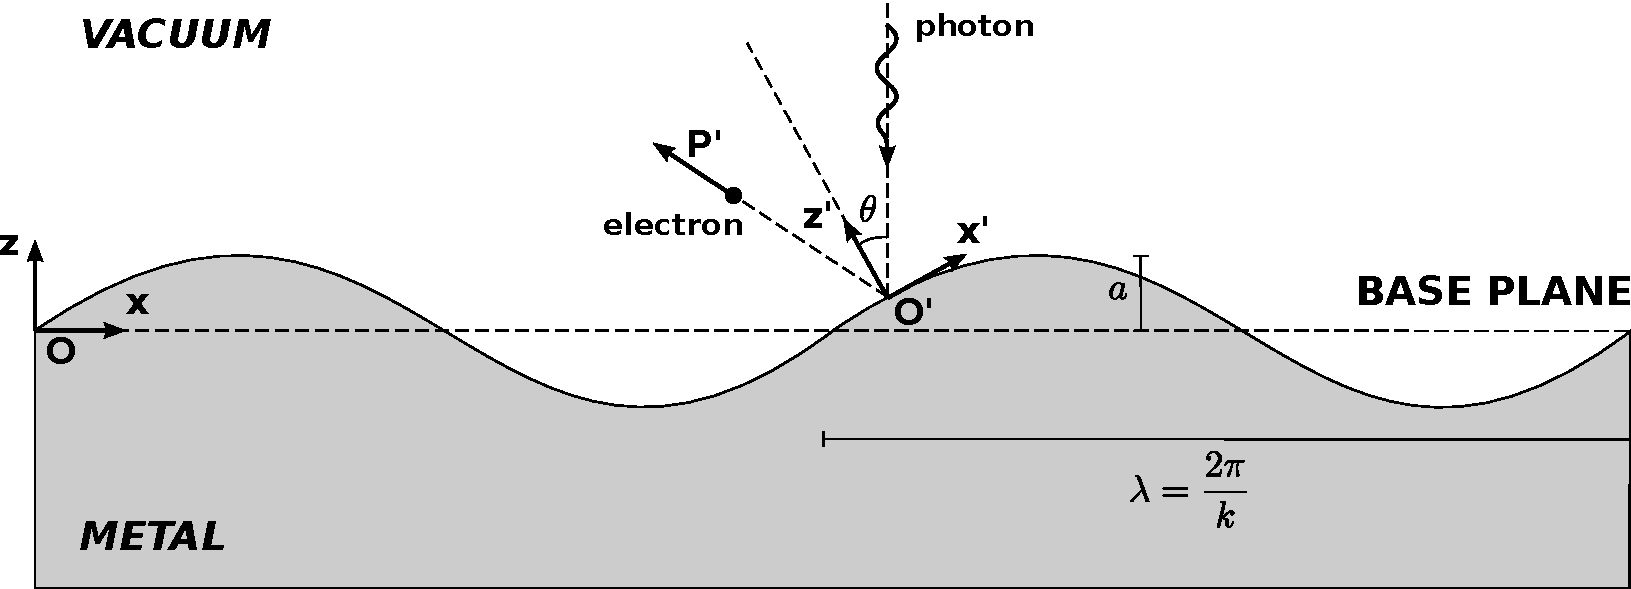
\includegraphics[width=0.9\textwidth]{coor_2D}
\caption{\label{fig:coor_2D} 2D 正弦表面的体发射示意图。坐标系统和参数的定义见图中标注。}
\end{figure}

如在节 \ref{ss:gmpsf} 中解释的那样,考虑在点 \textbf{P} 的入射,假设在全局坐标系下一个从点 \textbf{P} 发射出来的电子的横向和纵向动量分别为 $p_x, p_z$,应用 2D 旋转矩阵,我们有:
\[
\left(\begin{array}{c}
p_x\\
p_z
\end{array}\right)=
\left(\begin{array}{cc}
\cos\theta & -\sin\theta\\
\sin\theta & \cos\theta 
\end{array}\right)
\left(\begin{array}{c}
p_x^{\prime}\\
p_z^{\prime}
\end{array}\right)
\]
角度 $\theta$ 是从 z 轴到点 \textbf{P} 法向的夹角,且 $p_x^{\prime}, p_z^{\prime}$ 分别是发射电子在局部坐标系下的横向和纵向动量。上面的方程描述了发射角分散效应是如何影响横向动量,进而导致热发射度增长的。

现在考虑横向电场对发射度造成的影响。首先需要知道表面上横向电场的分布。有如下结论:定义 $\xi=ak$,那么若 $\xi$ 远小于 1,则正弦表面附近的电场可以写成下面形式:
\begin{eqnarray*}
E_x &=& E\xi\cdot e^{-kz}\sin kx \\
E_z &=& E\left(1+\xi e^{-kz}\cos kx\right)
\end{eqnarray*}
令 $A = eE/m$,可以证明,电子的横向动量近似满足下面的方程:
\[
p_{\infty}-p_0 = m\sqrt{\dfrac{\pi A}{2k}}\xi\sin kx
\]
其中 $p_{\infty}$ 是经历了阴极表面场后电子的最终横向动量。注意这里的横向动量应从极限的角度理解,即假定电子向 z 运动无穷远后,表面场对其横向的积分作用。事实上,电子的横向动量在离开表面几微米后就非常接近极限了。

将表面离散效应和横向电场效应叠加起来,就可以获得最终的 $p_x$ 的表达式:
\[
p_x = p_x^{\prime}\cos\theta-p_z^{\prime}\sin\theta + m\sqrt{\dfrac{\pi A}{2k}}\xi\sin kx
\]
其中:
\begin{eqnarray*}
\cos\theta &=&\dfrac{1}{\sqrt{1+\xi^2\sin^2kx}} \approx 1-\dfrac{1}{2}\xi^2\sin^2kx \\
\sin\theta &=&\dfrac{-\xi\sin kx}{\sqrt{1+\xi^2\sin^2kx}} \approx -\xi\sin kx
\end{eqnarray*}

将上面结果代入式 \ref{eq:emit_def},令 $p_C = m\sqrt{\pi A/2k}$($p_C$ 有动量的量纲),就得到式 \ref{eq:emit_2d} 所示的最终粗糙度发射度。这里我们定义式 \ref{eq:emit_2d} 中的方括号中的项的平方根为发射度增长因子 $\eta$,于是式 \ref{eq:emit_2d} 可以被重写为 $\varepsilon_x=\eta\cdot\varepsilon_{D, x}$。
\begin{equation}
\varepsilon_x^2 = \varepsilon_{D, x}^2\left[1+\dfrac{1}{2}\xi^2\left(\dfrac{\aver{\left(p_z^{\prime}+p_C\right)^2}}{\aver{{p_x^{\prime}}^2}}-1\right)\right]
\label{eq:emit_2d}
\end{equation}

当外场强度为 0 时,公式 \ref{eq:emit_2d} 就退化为表面离散效应粗糙度热发射度公式 \ref{eq:emit_2d_d};当 $p_z^{\prime} \ll p_C$ 时,式中的 $p_z^{\prime}$ 项可以忽略,从而公式 \ref{eq:emit_2d} 退化为横向电场效应粗糙度热发射度公式 \ref{eq:emit_2d_a}。
\begin{eqnarray}
\varepsilon_x^2 &\approx& \varepsilon_{D, x}^2\left(1+\frac{1}{2}\xi^2\right)\label{eq:emit_2d_d}\\
\varepsilon_x^2 &\approx& \varepsilon_{D, x}^2\left(1+\frac{3\pi e}{4}\cdot\frac{a^2kE}{\hbar\omega-\phi_{\text{eff}}}\right)\label{eq:emit_2d_a}
\end{eqnarray}

在式 \ref{eq:emit_2d} -- \ref{eq:emit_2d_a} 中代入表 \ref{tab:rough} 中的典型微观和宏观粗糙度参数,就可以看出对于微观粗糙度而言,发射度增长因子为 1.08,但是对于宏观粗糙度,发射度增长因子高达 1.35,这就意味着发射度增长主要是由宏观粗糙度导致的。分别保持 $\xi$ 和 $a$ 不变,画出粗糙度的空间周期 $\lambda$ 和发射度增长因子 $\eta$ 的关系,就得到图 \ref{fig:comp}。

\begin{figure}[htbp]
\centering
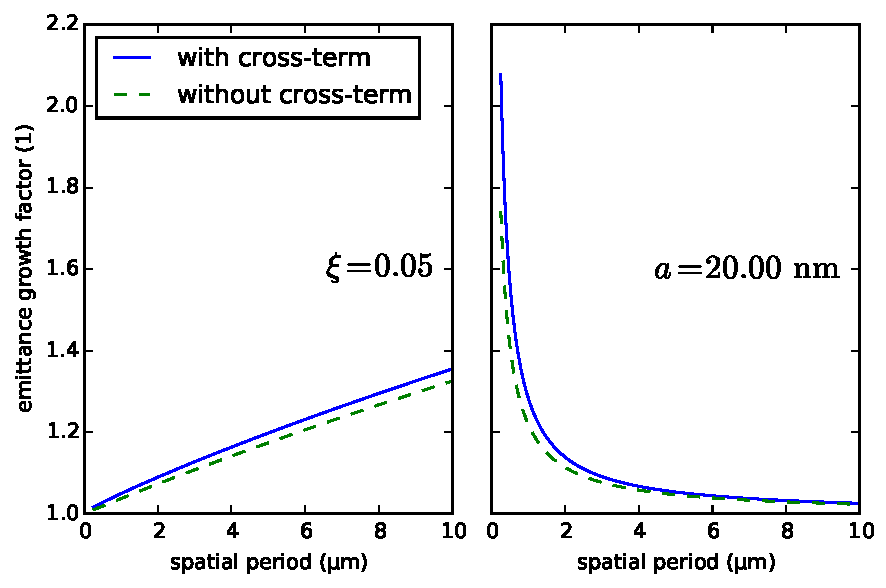
\includegraphics[width=0.7\textwidth]{comp}
\caption{\label{fig:comp} 2D 正弦表面上发射度增长因子与空间周期的关系。表面场强为 50\,MV/m。 左图是保持表面纹理的比例不变(即梯度不变,$\xi=0.05$);右图为保持表面振幅不变($a=20.00\,\text{nm}$)。}
\end{figure}

正如图 \ref{fig:comp} 中左图的实线所示,当等比例放缩表面纹理时,发射度增长因子和表面粗糙度空间周期是正相关的,这也验证了发射度增长的主要贡献来自宏观粗糙度的结论。我们也在图 \ref{fig:comp} 中检验了计算粗糙度热发射度时忽略表面离散效应和横向电场效应之间的耦合所造成的偏差,如图中虚线所示。容易看出实线和虚线间在某些空间周期时有着可观的差距,进一步的计算结果表明忽略两种效应耦合所造成的发射度增长的相对误差可达 10\%,这表明计算粗糙度热发射度时直接忽略两种效应的耦合有时是不合适的。

图 \ref{fig:comp} 说明了两个规律:1)阴极表面起伏越小,粗糙度热发射度增长越小;2)当阴极表面形状不变时,尺度越大,发射度增长就越大。图 \ref{fig:contour} 给出了一个关于空间周期,粗糙度振幅和发射度增长因子之间的更完整的理解。

\begin{figure}[htbp]
\centering
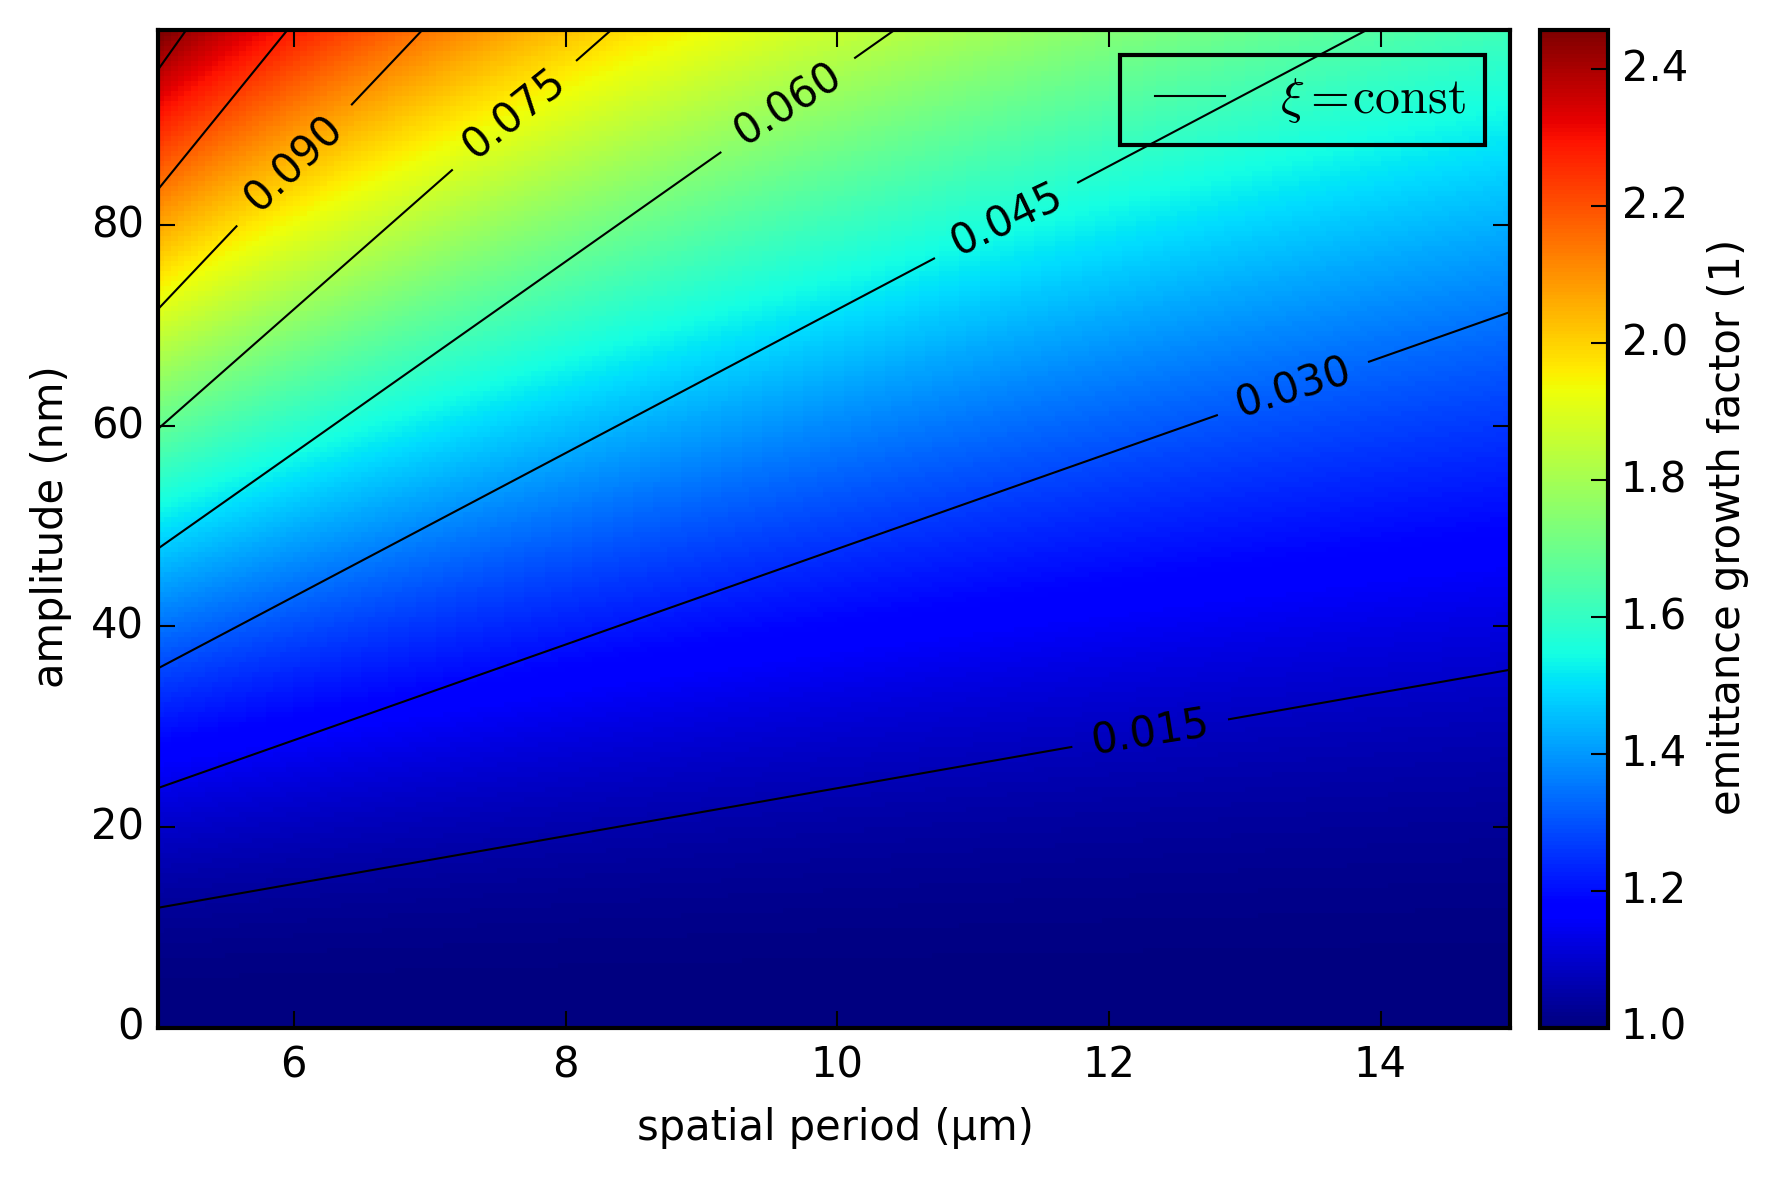
\includegraphics[width=0.6\textwidth]{contour}
\caption{\label{fig:contour} 发射度增长因子与表面粗糙度空间周期和振幅的关系。注意图中的黑色实线是表面形状(相同的形状 $\xi$ 相等)的等位线,而不是发射度增长因子的等位线,发射度增长因子相同则在图中颜色相同。}
\end{figure}

\subsection{\label{ss:2dr}2D 随机缓变粗糙表面}
现在我们研究 2D 随机缓变粗糙表面的情形,坐标系统如图 \ref{fig:coor_2Dr} 所示。
\begin{figure}[htbp]
\centering
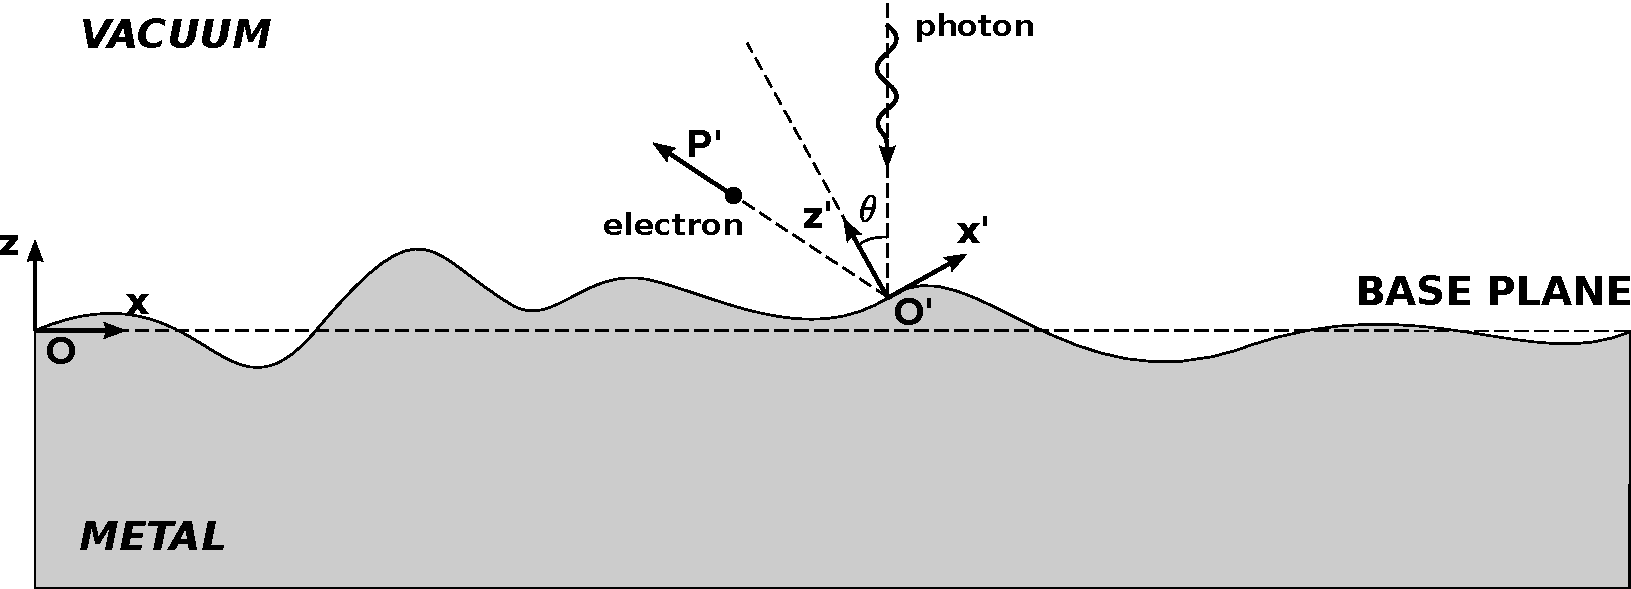
\includegraphics[width=0.9\textwidth]{coor_2Dr}
\caption{\label{fig:coor_2Dr} 2D 随机缓变粗糙表面的体发射示意图。坐标系统和参数的定义见图中标注。}
\end{figure}\\
计算 2D 随机缓变粗糙表面的粗糙度热发射度的思路与节 \ref{ss:2d} 中相同。表面离散效应造成的动量增长计算与节  \ref{ss:2d} 中的完全一致,所以我们跳过该部分而直接考虑横向电场效应部分。

假设表面形态函数为:
\[
z = R(x)
\]
我们选取基平面使得 $\langle R(x)\rangle=0$。和之前一样,想要计算横向场导致的横向动量增长,我们需要获取阴极表面附近的横向场分布。

\subsubsection{2D 随机缓变粗糙表面附近的电场分布}
受到 2D 正弦表面场分布计算的启发,我们可以假定在光阴极表面 $z = R(x)$ 与无穷远 $z = +\infty$ 之间的电势满足下面的近似形式:
\[
\phi(x, z) = z + \int dkC(k)\cdot e^{jkx-|k|z}
\]
上面的形式自动满足拉普拉斯方程 $\Delta\phi = 0$ 和 $z=\infty$ 处的边界条件 $\phi|_{z=d}=d, d\to\infty$,这里我们采用了归一化电场强度。现在考虑光阴极表面 $z=R(x)$ 处的边界条件。电势 $\phi$ 必须满足:
\[
\phi(x, z)\big|_{z=R(x)} = R(x) + \int dkC(k)\cdot e^{jkx-|k|R(x)} \equiv 0
\]
由于该表面为式 \ref{eq:def_gus} 所定义的随机缓变粗糙表面,$|k|R(x)$ 应该是一阶小量。将 $e^{-|k|R(x)}$ 做泰勒展开并保留一阶项就成为 $1-|k|R(x)$,代入上面的边界条件,就有:
\[
R(x) + \int dkC(k)\cdot e^{jkx} = O(1) \approx 0
\]
对 $R(x)$ 进行傅里叶展开:
\[
R(x) = \int dkR(k)\cdot e^{jkx}
\]
比较 $R(x)$ 的两个表达式,容易看出 $C(k) = -R(k)$,因此我们有二维随机缓变粗糙表面附近的电势 $\phi$ 的一阶近似表达式:
\begin{equation}
\label{eq:2d-pot}
\phi(x, z) = z - \int dkR(k)\cdot e^{jkx-|k|z}
\end{equation}

\begin{figure*}[htbp]
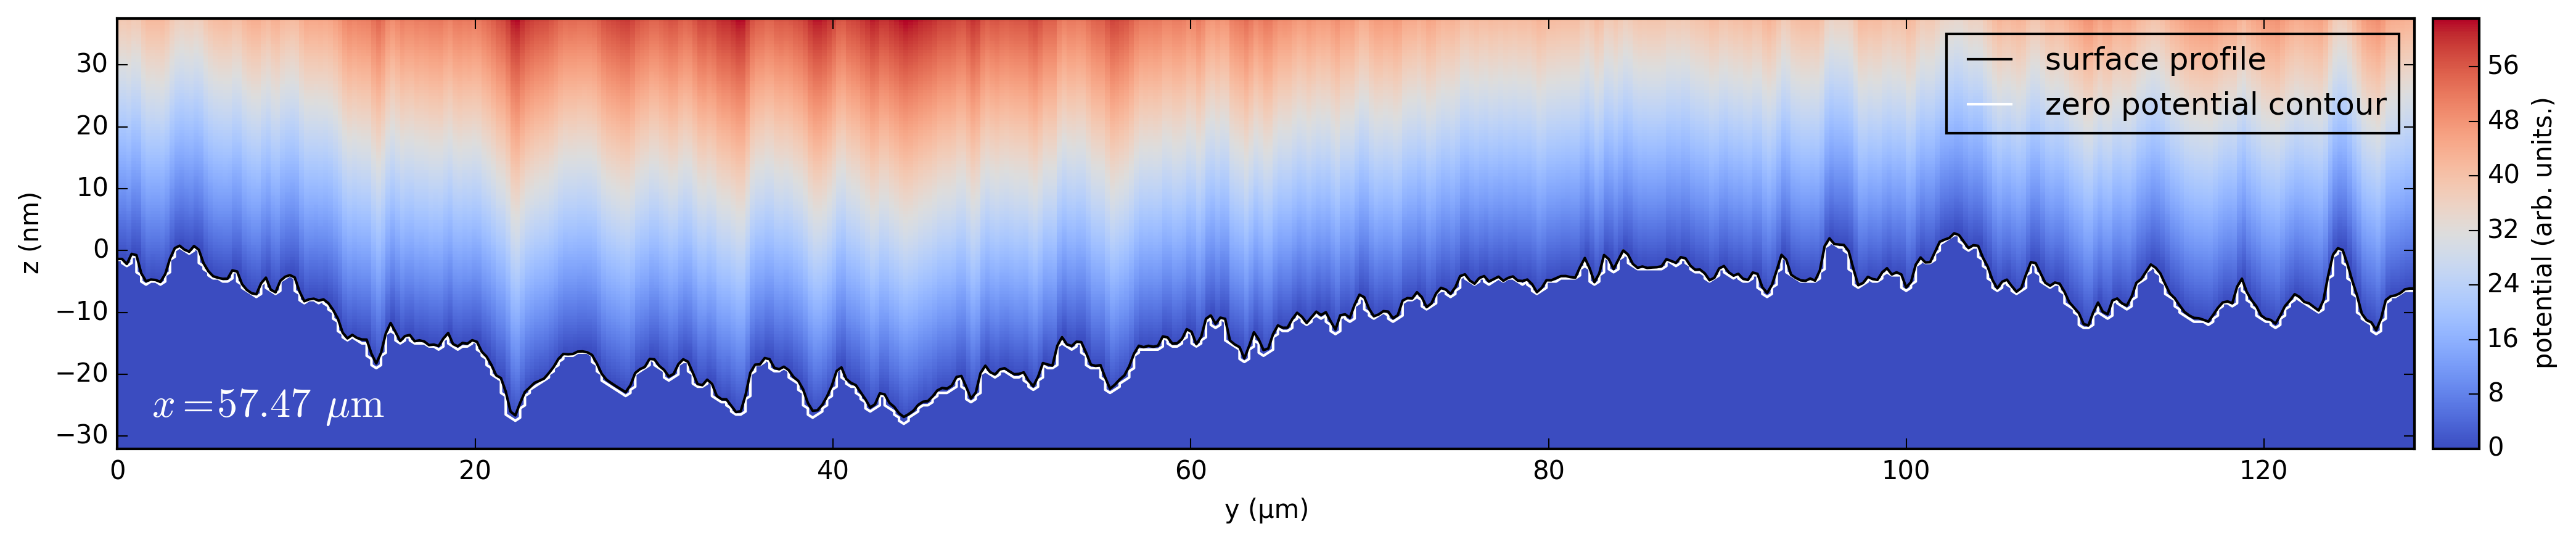
\includegraphics[width=\textwidth]{potential}
\caption{\label{fig:potential} 
验证电势一阶近似表达式的精确度。采用图 \ref{fig:conf} 所示的真实光阴极表面的沿 $x=57.47\,\mu\text{m}$ 的一个纵截面,该截面阴极表面轮廓用黑色实现描出;图中的白色实线为式 \ref{eq:2d-pot} 给出的解析公式的零势能面(对于 2D 情形而言是一条曲线),从图中可见看到,阴极表面轮廓和解析的零势能面几乎完全重合,这就验证了电势一阶近似表达式的精确性。}
\end{figure*}

为了验证上面的近似公式,我们选择了一个二维随机缓变粗糙表面,同时画出表面轮廓和近似的电势图。由于推导中我们假设阴极表面电势为 0,因此近似公式中的零势能面就描绘了解析的表面轮廓。实际的表面轮廓与解析的表面轮廓越接近,该一阶近似公式就越精确。二者的比较见图 \ref{fig:potential}。

从图 \ref{fig:potential} 中可以看到,二维随机缓变粗糙表面附近的电势一阶近似表达式是足够精确的。利用电势和电场间的关联 $\bm{E}=-\nabla\phi$,就可以得到表面附近的近似电场分布:
\begin{eqnarray*}
E_x &=& j\int dk\cdot kR(k)\cdot e^{jkx-|k|z} \\
E_z &=& -1-\int dk\cdot |k|R(k)\cdot e^{jkx-|k|z}
\end{eqnarray*}

\subsubsection{2D 随机缓变粗糙表面的粗糙度热发射度}

现在假定表面场强为 $E$,由牛顿第二定律可以写出:
\begin{eqnarray}
p_{\infty}-p_0 &=& m\sqrt{\dfrac{A}{2}}\cdot\int-\dfrac{E_x}{\sqrt{z}}\,dz\nonumber\\
&=& -jm\sqrt{\dfrac{\pi A}{2}}\cdot\int dk \dfrac{k}{\sqrt{|k|}}R(k)\cdot e^{jkx}\label{eq:p_field}
\end{eqnarray}
代入统计意义发射度公式计算可得最终发射度为:
\begin{equation}
\varepsilon_x^2 = \varepsilon_{D, x}^2\left[1-\aver{{R^{\prime}}^2}+\dfrac{\aver{\left(p_z^{\prime}\cdot R^{\prime}+jm\sqrt{\dfrac{\pi A}{2}}\displaystyle\cdot\int dk \dfrac{k}{\sqrt{|k|}}R(k)\cdot e^{jkx}\right)^2}}{\aver{{p_x^{\prime}}^2}}\right]
\label{eq:emit_2dr}
\end{equation}

为验证式 \ref{eq:emit_2dr} 的正确性,我们考虑节 \ref{ss:2d} 中所考虑的特殊二维情形,即二维正弦表面 $R(x) = a\cos k_0x$,为推导方便这里假定 $k_0>0$。令:
\[
I(x) = jm\sqrt{\dfrac{\pi A}{2}}\displaystyle\cdot\int dk \dfrac{k}{\sqrt{|k|}}R(k)\cdot e^{jkx}
\]
而 $R(k)=\frac{a}{2}\left[\delta(k-k_0)+\delta(k+k_0)\right]$,因此:
\begin{eqnarray*}
I(x) &&= jm\sqrt{\dfrac{\pi A}{2}}\left[\frac{a}{2}\dfrac{k_0}{\sqrt{|k_0|}}e^{jk_0x}-\frac{a}{2}\dfrac{k_0}{\sqrt{|k_0|}}e^{-jk_0x}\right]\\
&&= m\sqrt{\dfrac{\pi A}{2k_0}}\cdot(-ak_0\sin k_0x) = p_C\cdot R^{\prime}
\end{eqnarray*}
从而:
\begin{eqnarray*}
\varepsilon_x^2 &&= \varepsilon_{D, x}^2\left[1-\aver{{R^{\prime}}^2}+\dfrac{\aver{\left(p_z^{\prime}\cdot R^{\prime}+I(x)\right)^2}}{\aver{{p_x^{\prime}}^2}}\right]\\
&&= \varepsilon_{D, x}^2\left[1+\aver{{R^{\prime}}^2}\left(\dfrac{\aver{\left(p_z^{\prime}+p_C\right)^2}}{\aver{{p_x^{\prime}}^2}}-1\right)\right]\\
&&= \varepsilon_{D, x}^2\left[1+\dfrac{1}{2}\xi^2\left(\dfrac{\aver{\left(p_z^{\prime}+p_C\right)^2}}{\aver{{p_x^{\prime}}^2}}-1\right)\right]
\end{eqnarray*}
结果与式 \ref{eq:emit_2d} 相同。这就意味着对于二维缓变正弦表面,公式 \ref{eq:emit_2dr} 退化为公式 \ref{eq:emit_2d},这样我们就验证了二维随机缓变粗糙表面粗糙度热发射度公式 \ref{eq:emit_2dr} 的可靠性。

另外,$I(x)$ 也可以被写成下面的等价形式:
\begin{equation}
I(x) = \frac{m}{2}\sqrt{\frac{A}{|x|}}\ast R^{\prime}(x)
\label{eq:conv}
\end{equation}
利用卷积定理以及下面恒等式:
\[
\mathcal{F}\left(\dfrac{1}{\sqrt{|x|}}\right) = \frac{\sqrt{2\pi}}{|k|}
\]
其中 $\mathcal{F}\left(f(x)\right) = \int f(x)e^{-jkx}dx$ 是 $f(x)$ 的傅里叶变换,我们就可以直接得到式 \ref{eq:emit_2d} 的结果。

\subsection{\label{ss:3d}3D 随机缓变粗糙表面}
采用和节 \ref{ss:2dr} 相似的思想,可以解决三维随机缓变粗糙表面上粗糙度热发射度计算的问题。假定三维随机缓变粗糙表面可用下式描述:
\[
z = R(x, y)
\]
依然选取基平面使得 $\langle R(x, y)\rangle=0$。

\subsubsection{3D 随机缓变粗糙表面附近的电场分布}
仿照二维情形,我们假定光阴极表面 $z = R(x, y)$ 和无穷远 $z = +\infty$ 之间的电势有下面的近似形式:
\[
\phi(x, y, z) = z + \int dk_xdk_yC(k_x, k_y)\cdot e^{j(k_xx+k_yy)-kz}
\]
其中 $k=\sqrt{k_x^2+k_y^2}$。容易证明上面的形式自动满足拉普拉斯方程和无穷远处边界条件。结合阴极表面的边界条件,我们有 $C(k_x, k_y)=-R(k_x, k_y)$,其中 $R(k_x, k_y)$ 是 $R(x, y)$ 的傅里叶变换系数。于是电势可写成:
\[
\phi(x, y, z) = z - \int dk_xdk_yR(k_x, k_y)\cdot e^{j(k_xx+k_yy)-kz}
\]
进而电场具有以下形式:
\begin{eqnarray*}
E_x &=& j\int dk_xdk_y\cdot k_xR(k_x, k_y)\cdot e^{j(k_xx+k_yy)-kz} \\
E_y &=& j\int dk_xdk_y\cdot k_yR(k_x, k_y)\cdot e^{j(k_xx+k_yy)-kz} \\
E_z &=& -1-\int dk_xdk_y\cdot kR(k_x, k_y)\cdot e^{j(k_xx+k_yy)-kz}
\end{eqnarray*}

\subsubsection{3D 随机缓变粗糙表面的粗糙度热发射度}
现在考虑发射光电子的横向动力学,有:
\begin{eqnarray}
p_{\infty}-p_0 &=& m\sqrt{\dfrac{A}{2}}\cdot\int-\dfrac{E_x}{\sqrt{z}}\,dz\\\label{eq:p_field_3d}
&=& -jm\sqrt{\dfrac{\pi A}{2}}\cdot\int dk_xdk_y\dfrac{k_x}{\sqrt{k}}R(k_x, k_y)\cdot e^{j(k_xx+k_yy)}\nonumber
\end{eqnarray}

类似节 \ref{ss:2dr},不难推出三维随机缓变粗糙表面光阴极的粗糙度热发射度如式 \ref{eq:emit_3d} 所示。

\begin{equation}
\varepsilon_x^2 = \varepsilon_{D, x}^2\left[1-\aver{\partial_x^2R}+\dfrac{\aver{\left(p_z^{\prime}\cdot\partial_xR+jm\sqrt{\dfrac{\pi A}{2}}\displaystyle\cdot\int dk_xdk_y\dfrac{k_x}{\sqrt{k}}R(k_x, k_y)\cdot e^{j(k_xx+k_yy)}\right)^2}}{\aver{{p_x^{\prime}}^2}}\right]
\label{eq:emit_3d}
\end{equation}

和 2D 情形类似,将 $E = 0$ 代入式 \ref{eq:emit_3d},就可以得到三维表面离散效应粗糙度热发射度式 \ref{eq:emit_3d_d}。
\begin{equation}
\varepsilon_x^2 = \varepsilon_{D, x}^2\Big(1+\aver{\partial_x^2R}\Big)
\label{eq:emit_3d_d}
\end{equation}
由傅里叶能量守恒定律,$\aver{\partial_x^2R}$ 项可以被写成下面的等价形式:
\[
\left\langle \partial_x^2 R \right\rangle = \dfrac{\displaystyle\iint_{F(S)} k_x^2\left|R(k_x, k_y)\right|^2dk_xdk_y}{\displaystyle\iint_{S} dxdy}
\]
注意到空间谐波振幅 $|R(k_x, k_y)|$ 和空间谐波波数 $k_x$ 的乘积即为形状参数 $\xi$,而在 2D 正弦表面情形中,$\xi$ 参数正比于表面离散效应对粗糙度热发射度的贡献,因此这个对 2D 正弦表面成立的结论对于一般的随机缓变三维表面也成立,这同时意味着 2D 和 3D 的结果是自洽的。

尽管 3D 随机表面粗糙度热发射度形式上比 2D 正弦表面的要复杂,我们依然可以从公式 \ref{eq:emit_3d} 中得到一些有用的规律。例如,我们考虑发射度增长因子 $\eta$ 随外加电场强度 $E$ 的关系,将式 \ref{eq:emit_3d} 对 $E$ 展开就有:
\[
\eta^2 = aE+b\sqrt{E}+c
\]
这里 $a, b$ 和 $c$ 是只与阴极表面形状相关的参数。一些实验结果已经验证了 $E$ 和 $\varepsilon$ 具有类似的二次关系。

\section{\label{s:num}数值模拟验证}
\subsection{光阴极的量子效率与表面形态的关系}
在节 \ref{ss:gmpsf} 中,计算发射度时我们忽略了相对量子效率(或发射权重) $W(\theta)$ 与该点入射光子与表面法向之间夹角 $\theta$ 之间的关联,现在详细研究这二者之间的关系。铜光阴极的反射率 $R(\theta)$ 与发射权重 $W(\theta)$ 与入射角 $\theta$ 之间的关系如图 \ref{fig:weight} 中所示。
\begin{figure}[htbp]
\centering
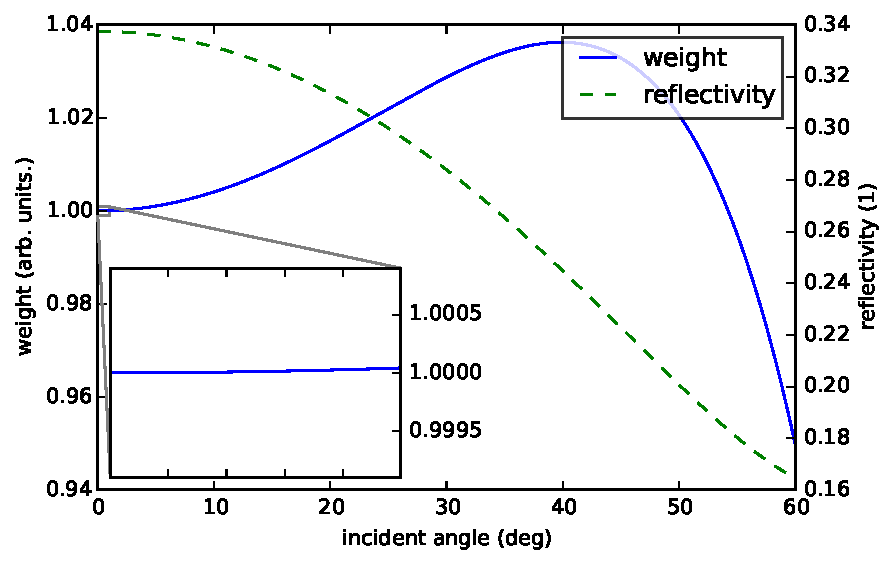
\includegraphics[width=0.6\textwidth]{weight}
\caption{\label{fig:weight} 相对量子效率 $W(\theta)$ 与反射率 $R(\theta)$ 与入射角 $\theta$ 之间的关系。相对量子效率 $W(\theta)$ 正比于阴极上该点处的光电子发射密度。图中图放大了 0 度到 1 度之间的相对量子效率曲线。}
\end{figure}
图 \ref{fig:weight} 也展示了 0 度到 1 度之间的相对量子效率曲线。容易看出在 1 度以下,相对量子效率基本是常数。这就是在发射度计算中忽略 $W(\theta)$ 和 $\theta$ 之间关系的原因。在以下的数值模拟中,$W(\theta)$ 也会被做为常量处理。

\subsection{\label{ss:sim-conf}数值模拟配置}
整个数值模拟程序采用 Python 编写,其模拟的场景如图 \ref{fig:conf} 所示。图中央区域的蓝红渐变区域代表激光入射区域,背景取自一块真实光阴极的表面的白光干涉仪测量结果。这块表面的空间频谱如图 \ref{fig:spec} 所示。阴极材料是无氧铜(阴极材料会影响阴极的逸出功,电子和光子的平均自由程,进而影响量子效率和发射度)。为模拟横向电场效应,我们在该表面引入了一个高场强电场,简单起见,采用了恒定场代替射频场,由于激光的脉冲长度远小于电子枪中射频场的周期,这个近似也是符合实际的。
\begin{figure}[htbp]
\centering
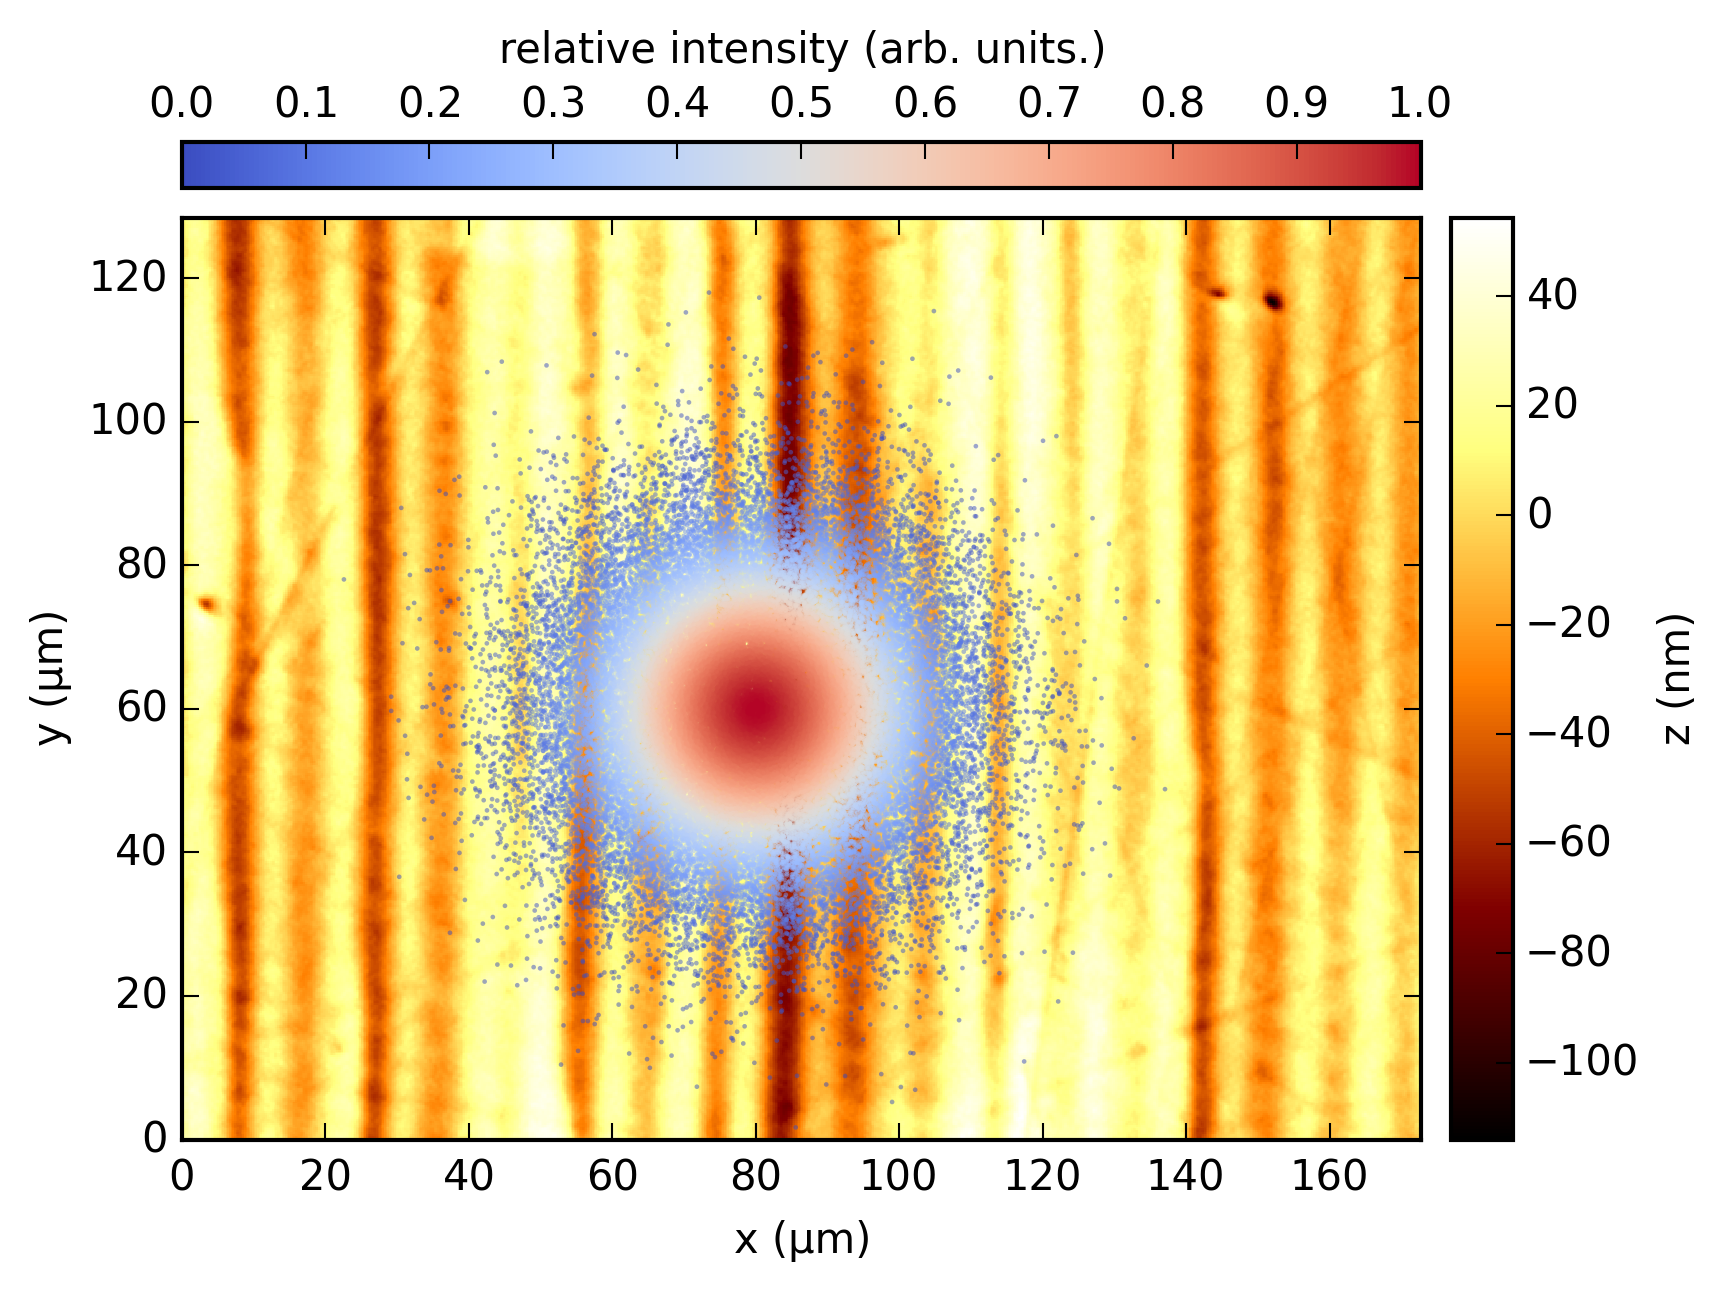
\includegraphics[width=0.6\textwidth]{configuration}
\caption{\label{fig:conf} 数值模拟配置。黄黑渐变的背景代表了模拟中所使用的表面的形态分布,中心附近红蓝渐变的区域描述了激光的横向功率密度分布。}
\end{figure}

\begin{figure}[htbp]
\centering
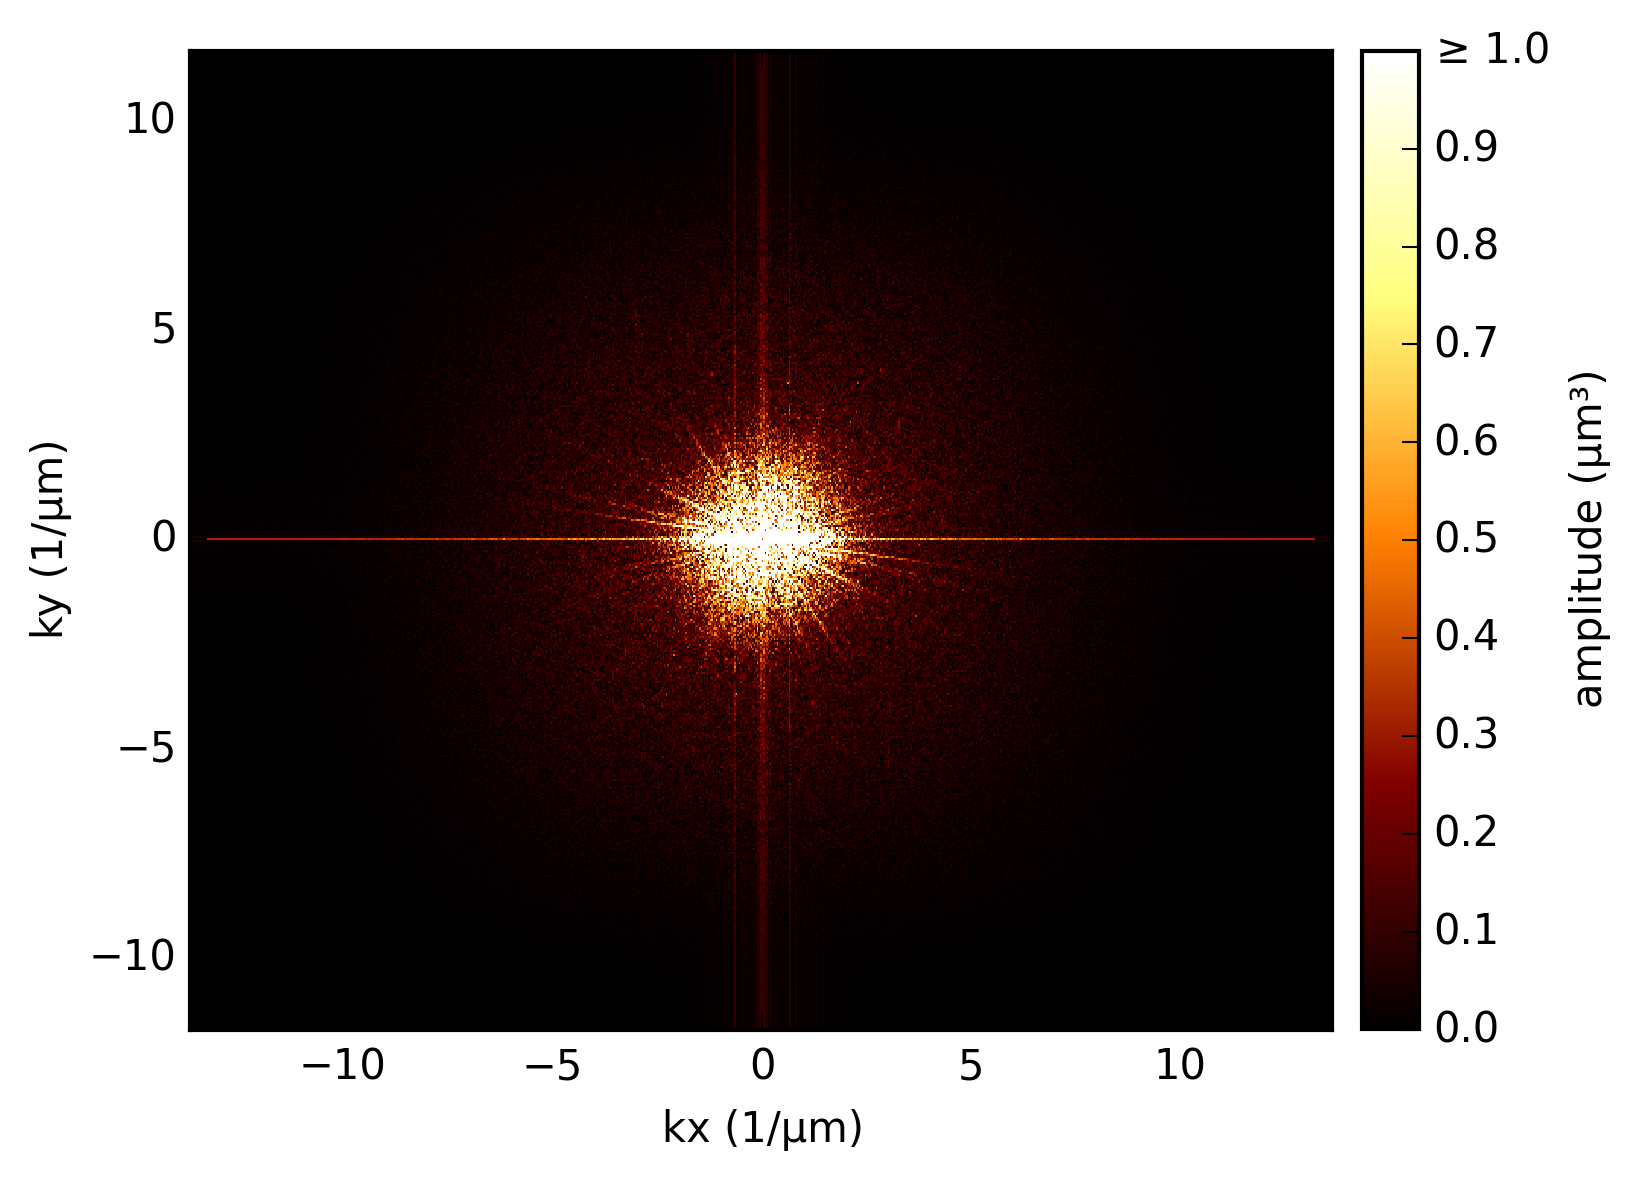
\includegraphics[width=0.6\textwidth]{spectrum}
\caption{\label{fig:spec} 模拟中采用的表面的空间频谱。为了使高频成分也可见,我们设置了饱和振幅为 1\,$\mu\text{m}^{3}$,也就是说变换后所有幅度大于 1\,$\mu\text{m}^{3}$ 的空间分量其振幅都当作 1\,$\mu\text{m}^{3}$ 来绘制。}
\end{figure}

在上面的配置下,我们对阴极表面的光电子进行动力学模拟,之后对初始发射度与饱和发射度进行统计,从而获得不同模拟参数下的发射度增长因子。

\subsection{\label{ss:sim-prin}数值模拟原理}
粗糙度热发射度可以分为两部分,即表面离散效应和横向电场效应导致的热发射度,进行数值模拟时需要对二者分别处理。总体而言,模拟需要一块特定材料的粗糙表面,一个外加场强与一束激光。我们采用了一块真实铜阴极的表面形态数据(白光干涉仪测量得到)做为特定材料的粗糙表面,其光学参数可以查阅得到;为了生成阴极表面上的外加电场,应用了节 \ref{ss:3d} 中给出的电场分布公式;为获得被给定横向功率密度分布的激光照射而出射的初始电子束团,首先生成符合激光横向功率密度分布的二维位置序列,随后对每个位置赋予一个概率分布为该点动量点扩散函数(由于法向不同,表面各点的动量点扩散函数有微小差异)的随机动量,最后将位置序列与随机动量合并,就得到了符合初始电子束相空间的一组采样。

有了初始电子束团,需要对其进行动力学模拟以给出发射度演变过程,这可以应用 5 阶龙格库塔法对运动方程进行积分。出于统计的方便,我们采用了以纵向位置坐标 $z$ 做为积分变量的方式,而不是以时间 $t$ 做为积分变量。以 $z$ 为变量的电子运动方程为:
\begin{eqnarray*}
\frac{dp_x\,[\text{keV/c}]}{dz\,[\text{nm}]} &=& 511\times 10^{-6}\cdot\frac{E_0\,[\text{MV/m}]}{p_z\,[\text{keV/c}]}\cdot \hat{E}_x(x, y, z)\\
\frac{dx\,[\mu\text{m}]}{dz\,[\text{nm}]} &=& \frac{p_x\,[\text{keV/c}]}{p_z\,[\text{keV/c}]}\cdot 1\times 10^{-3}
\end{eqnarray*}
其中 $x$ 代表横向,$E_0$ 是阴极表面电场强度,$\hat{E}_x$ 是归一化横向电场分布。值得注意的是,考虑到缓变表面的特征与模拟的目的,我们选取了 $\mu$m 做为横向尺寸的单位,nm 做为纵向尺寸单位。

从阴极表面电场分布的公式上可看出,电场的横向分量随着到基平面距离的增大而指数衰减,因此光电子的横向动量一定会很快饱和。通过实际模拟发现,饱和距离可以选在距离基平面 5000\,nm 附近,我们就在饱和距离处进行发射度增长因子的统计。

\subsection{\label{ss:sim-res}数值模拟结果}
数值模拟参数参见表 \ref{tab:sim1},发射度演变结果见图 \ref{fig:sim1}。
\begin{table}[htbp]
\centering
\caption{\label{tab:sim1}
数值模拟中所用参数。}
\begin{tabular}{llll}
\toprule
参数 & 值 & 单位 & 描述\\
\midrule
$\lambda_l$ & 266.0 & nm & 激光波长 \\
l-dist & \text{均匀分布} & - & 激光横向分布 \\
$r_l$ & 20.0 & $\mu$m & 激光横向半径 \\
$x_l$ & 80.0 & $\mu$m & 激光入射中心横座标 \\
$y_l$ & 60.0 & $\mu$m & 激光入射中心纵座标 \\
mat & \text{无氧铜} & - & 光阴极材料 \\
$E_0$ & 50.0 & MV/m & 阴极表面有效电场强度 \\
$\phi_w$ & 4.31 & eV & 阴极逸出功 \\
$\phi_{\text{eff}}$ & 4.04 & eV & 阴极有效逸出功 \\
$E_F$ & 7.0 & eV & 材料费米能级 \\
$N$  & 10000 & - & 模拟所用粒子数 \\
$z_i$ & 0 & nm & 模拟起始位置 \\
$z_f$ & 5000.0 & nm & 模拟结束位置 \\
$dz$ & 10.0 & nm & 模拟步长 \\
\bottomrule
\end{tabular}
\end{table}

从图 \ref{fig:sim1} 中可看到,在运动过程中,束团相空间沿着 $x$ 方向逐渐扭曲。相空间扭曲的原因就是表面的横向电场,而正是相空间扭曲导致了发射度增长。分别对初始相空间和结束相空间进行统计,可以得到发射度增长因子:
\[
\eta_{s} = \frac{\varepsilon_f}{\varepsilon_i} = \frac{4.826\,\mu\text{m}\cdot\text{keV}/c}{4.623\,\mu\text{m}\cdot\text{keV}/c} = 1.044
\]
令人惊讶的是,发射度增长因子比大部分文献中报道的(1.5 $\sim$ 2)要小得多!我们的模拟结果说明了表面粗糙度效应可能并非实验中观测到的发射度增长的唯一原因。

\begin{figure}[htbp]
\centering
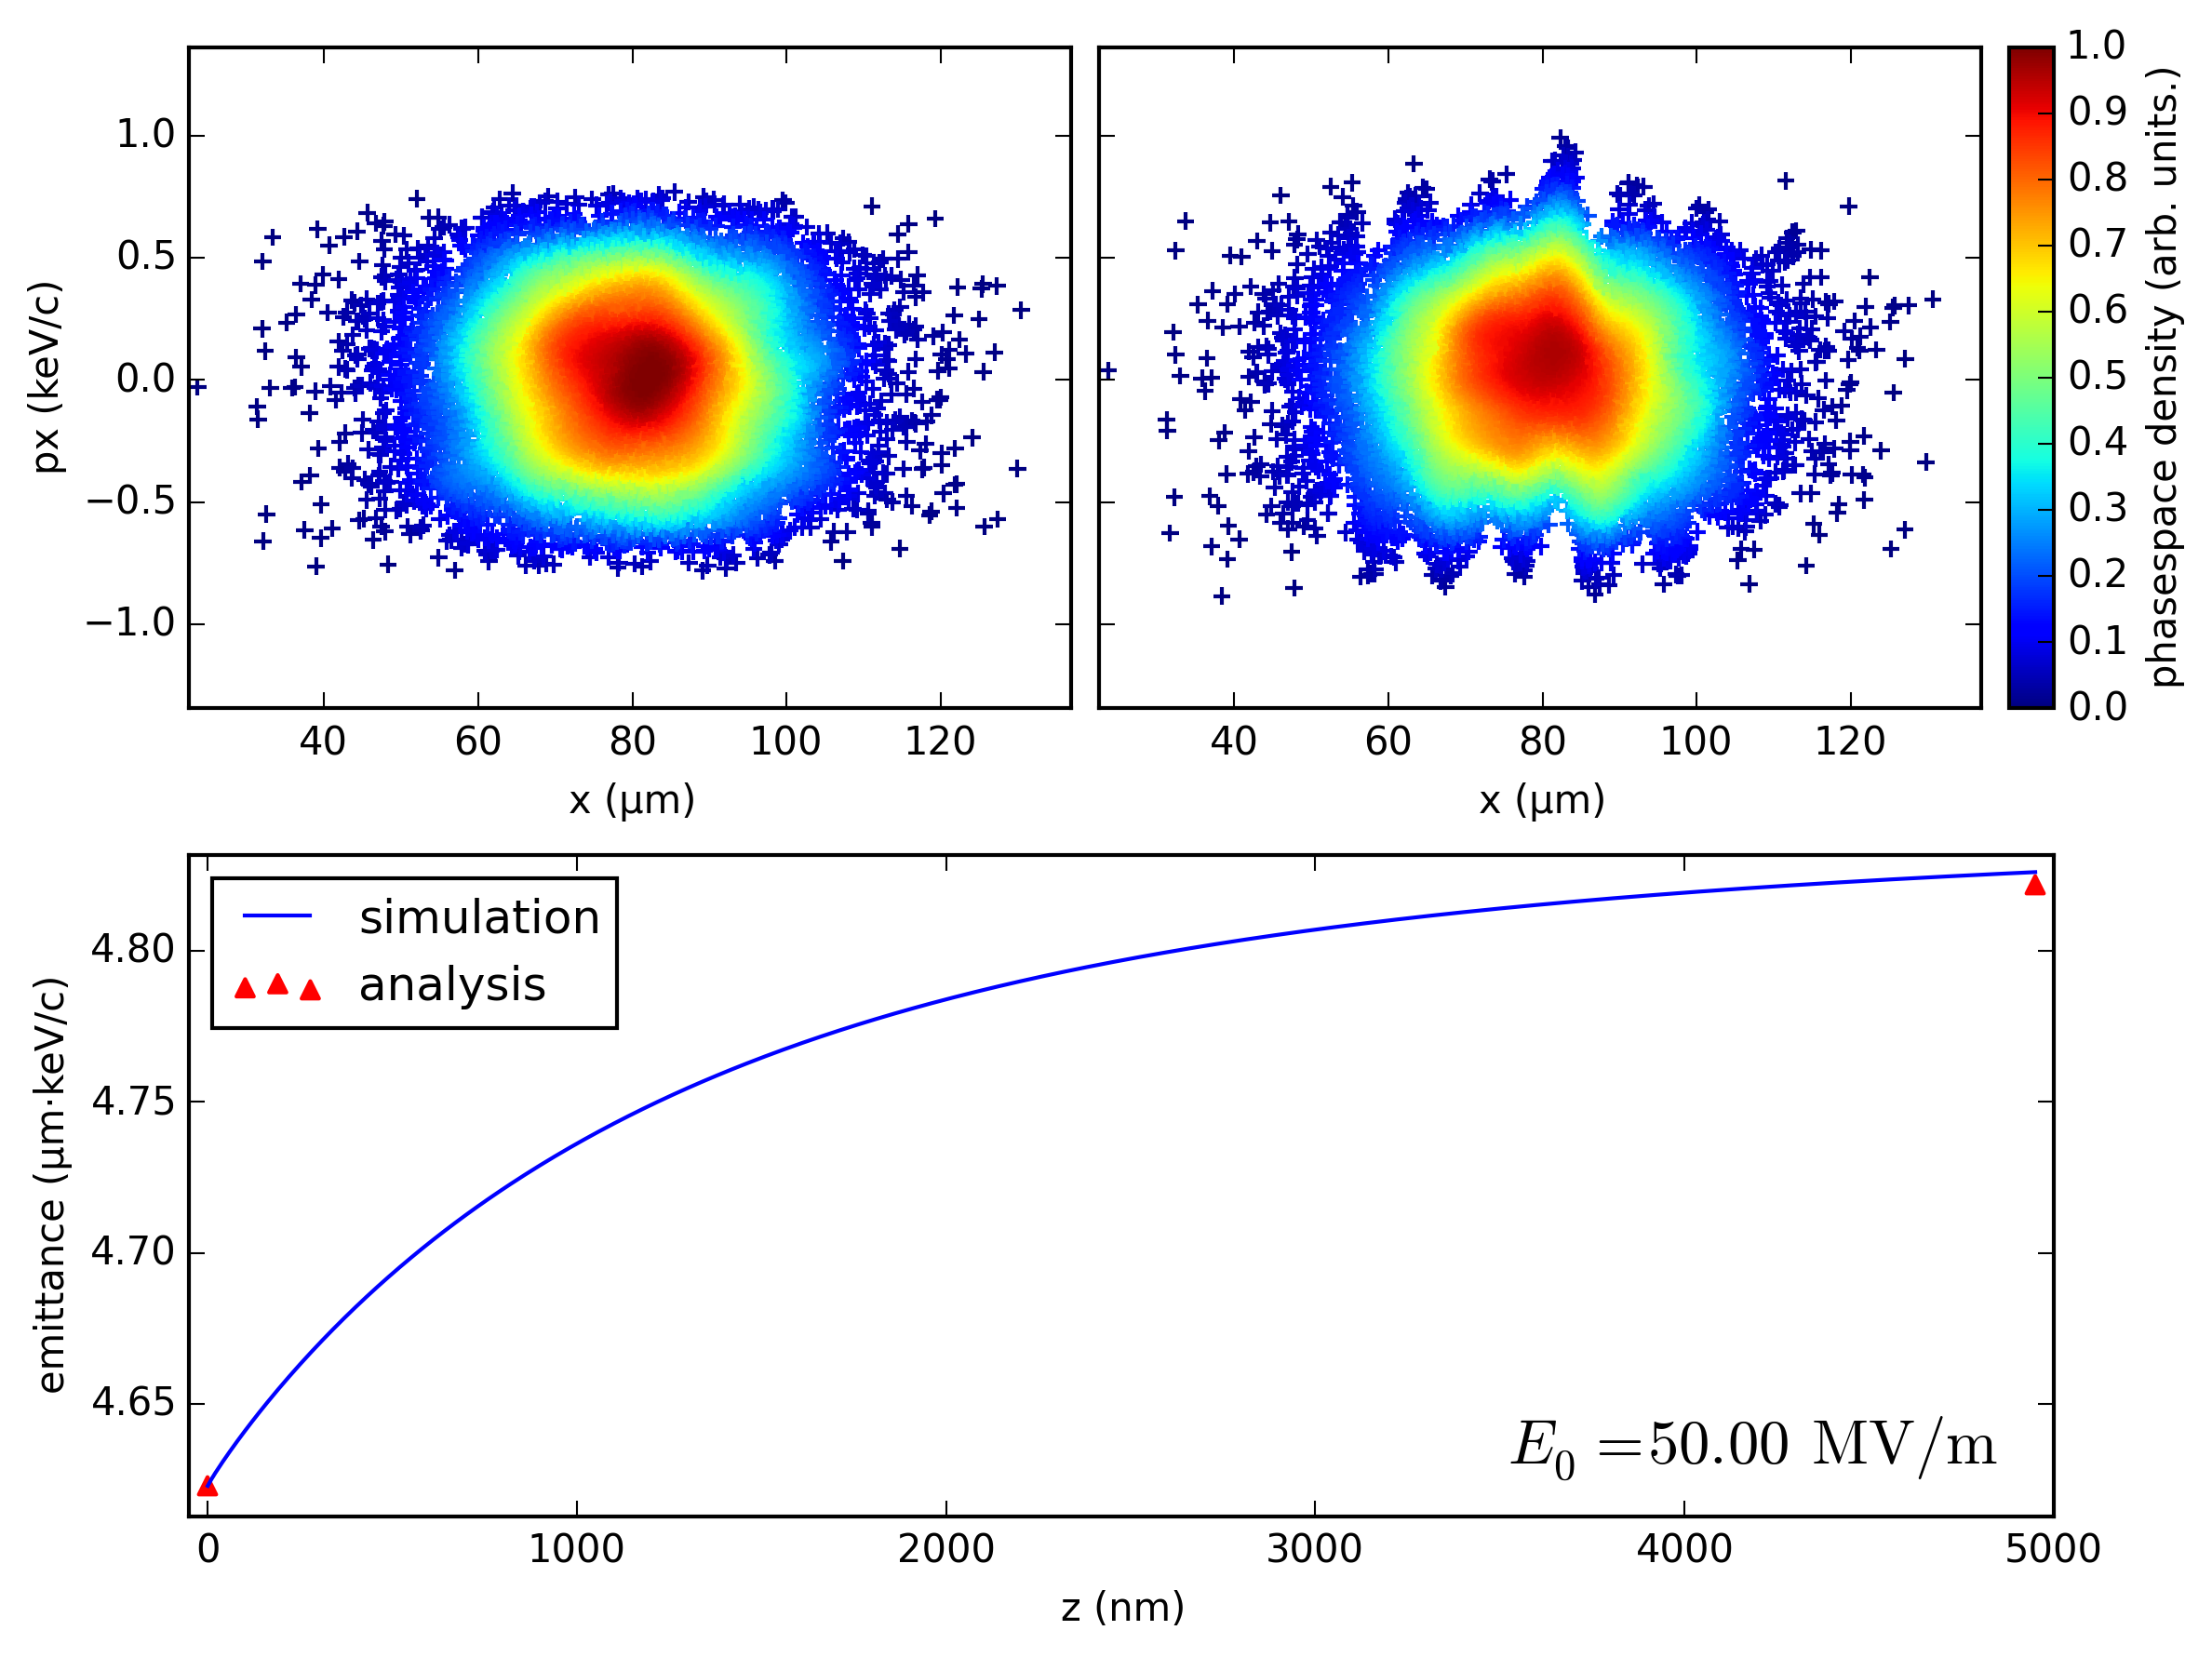
\includegraphics[width=0.6\textwidth]{simulation}
\caption{\label{fig:sim1} 
图 \ref{fig:conf} 中所示的粗糙铜阴极表面的电子束相空间与发射度演变的模拟结果。左上图是 $z=0\,\text{nm}$ 处的初始相空间分布,右上图是 $z=5000\,\text{nm}$ 处的最终相空间分布,下图是发射度 $\varepsilon_x$ 沿 $z$ 的演变,其中左右两个红色三角符号分别是解析初始发射度与解析饱和发射度。}
\end{figure}

\subsection{\label{ss:sim-res}数值模拟与解析结果的对比}
我们在图 \ref{fig:sim1} 中比较了粗糙度发射度的模拟结果与解析结果(见公式 \ref{eq:emit_3d})。图中的两个红色三角形符号代表解析结果:左边的是只考虑了表面离散效应的粗糙度热发射度,($\varepsilon_1$),右边则是将横向电场效应一起加入的粗糙度热发射度($\varepsilon_2$)。由于模拟中在产生初始电子束团时,已经包含了表面离散效应,而且采用了相同的电子束团进行理论计算和模拟模拟,因此 $\varepsilon_1$ 对于理论和模拟而言是完全相同的。

对于 $\varepsilon_2$,理论上说模拟结果应该比解析结果略小并且随着纵向位置 $z$ 的增大逐渐趋于解析结果,但是图 \ref{fig:sim1} 中却正相反。这可能是因为我们的模拟步长选得过大导致的,因为横向电场分布会随着 $z$ 的增大而衰减,所以运动方程积分会比真实的动量改变要大(因为龙格库塔法中每步所采用的外场都是上一时刻的场),进而导致模拟结果比解析结果略大。

尽管如此,解析公式给出的最终发射度增长因子为:
\[
\eta_a = \frac{\varepsilon_2}{\varepsilon_1} = \frac{4.822\,\mu\text{m}\cdot\text{keV}/c}{4.623\,\mu\text{m}\cdot\text{keV}/c} = 1.043
\]
可以看出解析结果与数值模拟结果相当接近,这就进一步验证了解析结果的可靠性。

应用粗糙度发射度的解析公式,发射度增长因子的计算速度可以大大提高,所以可以借助解析公式来探索阴极表面电场强度与发射度增长因子之间的关系。分析结果见图 \ref{fig:factor_comp} 中蓝色实线。图 \ref{fig:factor_comp} 说明,对于经过打磨的光阴极,其由于三维表面粗糙度造成的发射度增长是很小的,即使在阴极表面场高达 120\,MV/m 的情形下,发射度增长因子仍然小于 1.1。

\begin{figure}[htbp]
\centering
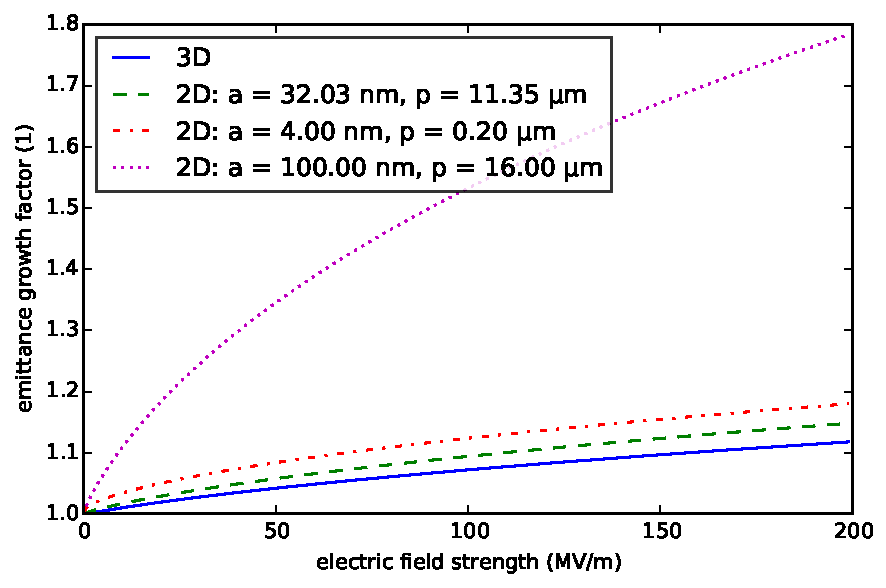
\includegraphics[width=0.6\textwidth]{factor_comp}
\caption{\label{fig:factor_comp} 2D 粗糙表面和 3D 粗糙表面的发射度增长因子对比。蓝色实线对应图 \ref{fig:conf} 中所示的粗糙阴极表面的发射度增长因子;绿色虚线代表粗糙度参数和 3D 粗糙表面相同的 2D 近似公式给出的增长因子;红色点划线和洋红色点虚线分别对应表 \ref{tab:rough} 中的微观粗糙度和宏观粗糙度参数对应的 2D 近似公式给出的增长因子。}
\end{figure}

图 \ref{fig:factor_comp} 中同时比较了若干粗糙度参数不同的 2D 正弦表面与 3D 随机缓变粗糙表面的发射度增长。对于 2D 正弦表面,我们采用了三组不同的粗糙度空间周期 $p$ 和粗糙度振幅 $a$,具体说明见图 \ref{fig:factor_comp} 题注。可以看出,在表面场强相同的情况下,2D 宏观粗糙度的发射度增长因子明显高于 3D 真实阴极表面的发射度增长因子。但是由于 3D 表面的粗糙度参数 $a$ 和 $p$ 与宏观粗糙度的参数有很大差异,这种比较并无太大意义。为了获得更有意义的比较结果,我们统计了图 \ref{fig:conf} 所示的粗糙表面的粗糙度参数,得到其 rms 粗糙度 $R_q$ 和 rms 平均空间波长 $\lambda_q$ 分别为 22.65\,nm 和 11.35\,$\mu$m。对应的 2D 正弦表面若想达到相同的粗糙度参数,其空间周期 $\lambda$ 和振幅 $a$ 需要满足下式:
\begin{eqnarray*}
&&a = \sqrt{2}R_q \\
&&\lambda = \lambda_q
\end{eqnarray*}
计算得到 $a=32.03\,\text{nm}$,$\lambda=11.35\,\mu\text{m}$。应用这组参数,画出对应的发射度增长因子曲线如图 \ref{fig:factor_comp} 中的绿色虚线所示。可以看出,对于拥有相同粗糙度参数的 3D 和 2D 表面,其发射度增长因子是非常接近的,但是 3D 情形总是比 2D 情形的发射度增长因子更小。这个现象的原因可能是 3D 表面的横向动量增长是分散在整个 x-y 平面的,但是 2D 表面的横向动量增长被限制在 x 方向,因此对于相同的粗糙度参数,2D 表面发射度增长总是高于 3D 情形。

粗糙度参数匹配的 2D 和 3D 表面的发射度增长因子的相似性给了我们一个估算真实三维阴极的粗糙度发射度增长上限的简单办法:首先计算真实阴极表面的粗糙度参数 $R_q$ 和 $\lambda_q$,随后将 $a=\sqrt{2}R_q$ 以及 $k=2\pi/\lambda_q$ 代入 2D 正弦表面粗糙度发射度公式 \ref{eq:emit_2d_a} 中,计算结果就是真实阴极粗糙度热发射度的上限。具体经验公式如式 \ref{eq:upperlimit} 所示。
\begin{equation}
\bar{\varepsilon}_{n, x}^2 = \sigma_x^2\cdot\left[\frac{\hbar\omega-\phi_{\text{eff}}}{3mc^2}+\frac{\pi e^2}{mc^2}\cdot\frac{R_q^2E}{\lambda_q}\right]
\label{eq:upperlimit}
\end{equation}

正如图 \ref{fig:factor_comp} 所示,无论 3D 表面还是与其粗糙度匹配的 2D 表面都不会造成显著的粗糙度热发射度增长(当阴极表面有效场强接近 150\,MV/m 时发射度增长也不超过 10\%)。这个事实证明在实验中观测到的较大发射度增长可能并不是主要由阴极表面粗糙度和阴极表面的高引出场强造成的,或许另有原因。

\section{小结}
本章我们首先引入了光阴极的点扩散函数,应用点扩散函数的观点验证了光电子动量分布与光子入射近似位置无关的假设。随后给出缓变粗糙表面的概念,推导并首次获得了随机缓变粗糙 2D 表面与 3D 表面的粗糙度热发射度的解析公式。通过对一个简单 2D 正弦表面的分析,我们讨论了表面离散效应与横向电场效应的耦合,并指出计算总粗糙度热发射度时不应随便忽略二者的耦合效应。

接着我们对一块真实阴极上光电发射过程中束团相空间及粗糙度热发射度的演化进行了数值模拟,以验证粗糙度热发射度解析公式。通过数值模拟,验证了解析公式给出的结果足够精确;同时也发现对于三维随机缓变粗糙表面及粗糙度参数与其匹配的二维缓变粗糙表面,表面粗糙度对于发射度增长的共享明显低于预期。甚至阴极表面场强高达 120\,MV/m 时,发射度增长因子也低于 1.1,与发射度测量的一系列实验的测量值 1.5 $\sim$ 2 有较大差距。因此我们猜想,实验中观测到的发射度大幅增长也许另有原因。

本章给出的粗糙度热发射度的理论与模拟结果也表明,对于一块经过机器精细打磨的阴极(表面 rms 起伏不超过 \SI{30}{nm},表面 rms 坡度不大于 \SI{3}{mrad}),在阴极表面电场不太高($\sim$ 50\,MV/m,该场强是 S 波段光阴极微波电子枪中的常用场强)其表面粗糙度造成的发射度增长可以忽略不计。这也说明在阴极加工时,要尽量避免手工打磨阴极,因为手工打磨阴极造成的粗糙度一般在百 nm 量级,有可能造成较大粗糙度热发射度。

%!TEX root = ../main.tex
\chapter{纳米表面光阴极亮度的理论与实验探究}
\label{chap:NPC}

\section{表面等离激元与纳米表面光阴极}

\section{纳米表面光阴极亮度测量的实验准备}

\section{纳米表面光阴极的电子产额测量}

\section{纳米表面光阴极的热发射度测量}

%!TEX root = ../main.tex
\chapter{高亮度空间分离双频电子枪的优化设计}
\label{chap:GA}
近年来理论和实验研究指出,在光阴极上产生笔形束(纵横比远大于 1 的束团)可以提高注入器出口处束流的横向亮度,且束流的峰值流强可以通过在电子枪后放置一个微波聚束器得到提高。我们将这个结果应用于 S 波段光阴极注入器中,提出了将一个高次谐波腔紧贴 S 波段电子枪放置,就可形成一个空间分离的双频电子枪,目标是实现 200\,pC 电荷量下注入器出口处达到 30\,A 峰值流强以及 0.2\,mm$\cdot$mrad 以下的发射度。

\begin{table}[htbp]
\caption{几个重要装置注入器出口束流参数的实验测量结果}
\centering
\begin{tabular}{lcccccl}
\toprule
波段 & 峰值场强 & 发射场强 & 枪电压 & 发射度 & 峰值流强 & 装置 \\
 & MV/m & MV/m & MV & $\mu$m & A & \\
\midrule
S-band & $\sim$ 100 & $\sim$ 50 & $\sim$ 5 & $\sim$ 0.2--0.45 & 20--50 & LCLS/PSI \\
L-band & $\sim$ 60 & $\sim$ 45 & $\sim$ 7 & $\sim$ 0.3 & 15 & PITZ \\
DC & $\sim$ 4 & $\sim$ 4 & $\sim$ 0.4 & $\sim$ 0.6 & 30 & Cornell \\
VHF & $\sim$ 20 & $\sim$ 20 & $\sim$ 0.8 & $\sim$ 0.45 & 30 & APEX \\
\bottomrule
\end{tabular}
\end{table}

\section{光阴极的极限热发射度}
如绪论中所述,光阴极注入器出口处的发射度已经逐渐趋近于光阴极表面的热发射度,因此如何进一步降低光阴极的热发射度就成为近年来的研究热点。下面我们就当前注入器中常用的两种束团发射状态:扁平束(pancake beam)和笔形束(cigar beam),探究一下光阴极的极限热发射度。在下面的叙述中,假设光阴极的光电发射为体发射,因此采用三步模型做理论推导。

\subsection{扁平束的极限热发射度}
Dowell 指出,利用三步模型可以得到光阴极的量子效率 QE 以及热发射度 $\varepsilon$ 如下:
\begin{eqnarray*}
\text{QE}(\omega) &\approx& \dfrac{1-R(\omega)}{1+\dfrac{\lambda_{\text{opt}}}{\lambda_{e-e}(\omega)}}\frac{(\hbar\omega-\phi_{\text{eff}})^2}{8\phi_{\text{eff}}(E_F+\phi_{\text{eff}})}\\
\varepsilon_{n,x} &=& \sigma_x\sqrt{\dfrac{\hbar\omega-\phi_{\text{eff}}}{3mc^2}}
\end{eqnarray*}
其中 $\phi_{\text{eff}}$ 为有效逸出功,满足:
\[
\phi_{\text{eff}} = \phi_{w} - e\sqrt{\frac{eE_0}{4\pi\varepsilon_0}}
\]
上式中 $\phi_{w}$ 为金属阴极的逸出功。若不考虑发射过程中束团的纵向空间电荷力,那么束团的热发射度可写做:
\begin{equation}
\varepsilon = \sigma_x\cdot\sqrt{\frac{\hbar\omega-\phi_w+e\sqrt{\frac{eE_0}{4\pi\varepsilon_0}}}{3mc^2}}
\label{eq:tot-emit-none}
\end{equation}
但是空间电荷限发射时,束团纵向空间电荷力几乎抵消了阴极表面场强,所以上面假设显然不能成立,下面计算考虑了纵向空间电荷效应的阴极热发射度。

假设阴极表面引出场强为 $E_0$,束团电荷量为 $Q$,激光横向分布为圆均匀分布,那么对于扁平束而言,空间电荷限对表面场强的减小最大为(考虑到镜像电荷作用):
\begin{equation}
E_{SC} \approx \frac{Q}{\varepsilon_0S} = \frac{Q}{\varepsilon_0\pi r^2}
\label{eq:e-sc-pancake}
\end{equation}
其中 $r$ 为激光半径,$S$ 为激光在阴极上的辐照面积。

为保证束团可以完整发射,最大空间电荷场 $E_{SC}$ 不能高于引出电场 $E_0$,也即:
\begin{equation}
E_0 \ge \frac{Q}{\varepsilon_0\pi r^2}
\label{eq:sc-limit}
\end{equation}
在光阴极电子枪中,引出场强 $E_0$ 被打火/击穿/暗电流大小等因素限制不能太大,对于 $S$ 波段光阴极电子枪而言,$E_0$ 一般可以取到 \SI{120}{MV/m}。

若考虑切片的空间电荷场对引出场强的减弱,且忽略不同切片的减弱不同的效应,就可以算出考虑了空间电荷场的束团发射度:
\begin{equation}
\varepsilon = \sigma_x\cdot\sqrt{\frac{\hbar\omega-\phi_w+e\sqrt{\frac{e\left(E_0-\frac{Q}{\varepsilon_0 S}\right)}{4\pi\varepsilon_0}}}{3mc^2}}
\label{eq:tot-emit-orig}
\end{equation}
其中 $Q$ 为总发射电荷量。

然而真实情形并非如此。由 Dowell 发射度公式及有效逸出功公式可知,对于发射时刻不同的切片,由于已发射电荷量 $q$ 不同,空间电荷力造成的阴极表面场减小也不同,从而其有效逸出功不同,导致其发射度也有差别。发射时刻越靠后的切片,其阴极表面场减小一般越强,发射度也就越小,当然,同时其量子效率也会降低。因此统计热发射度时,需要考虑各个切片发射度有差异的问题。

另外需要注意的是,肖特基效应造成逸出功降低是利用单电子发射模型推导的,而我们考虑的情形是束团中某个切片的发射过程,该切片发射时可能阴极表面已经存在一定的发射电荷,因此单电子发射给出的有效逸出功需要进行修正。

\subsubsection{切片中电子感受到的有效逸出功的修正}
考虑图 \ref{fig:schottky-mod} 中的发射过程,设整个束团发射长度为 $L$,我们考察纵向相对位置为 $\zeta$ 的切片在发射过程中感受到的电场。
\begin{figure}[htbp]
\centering
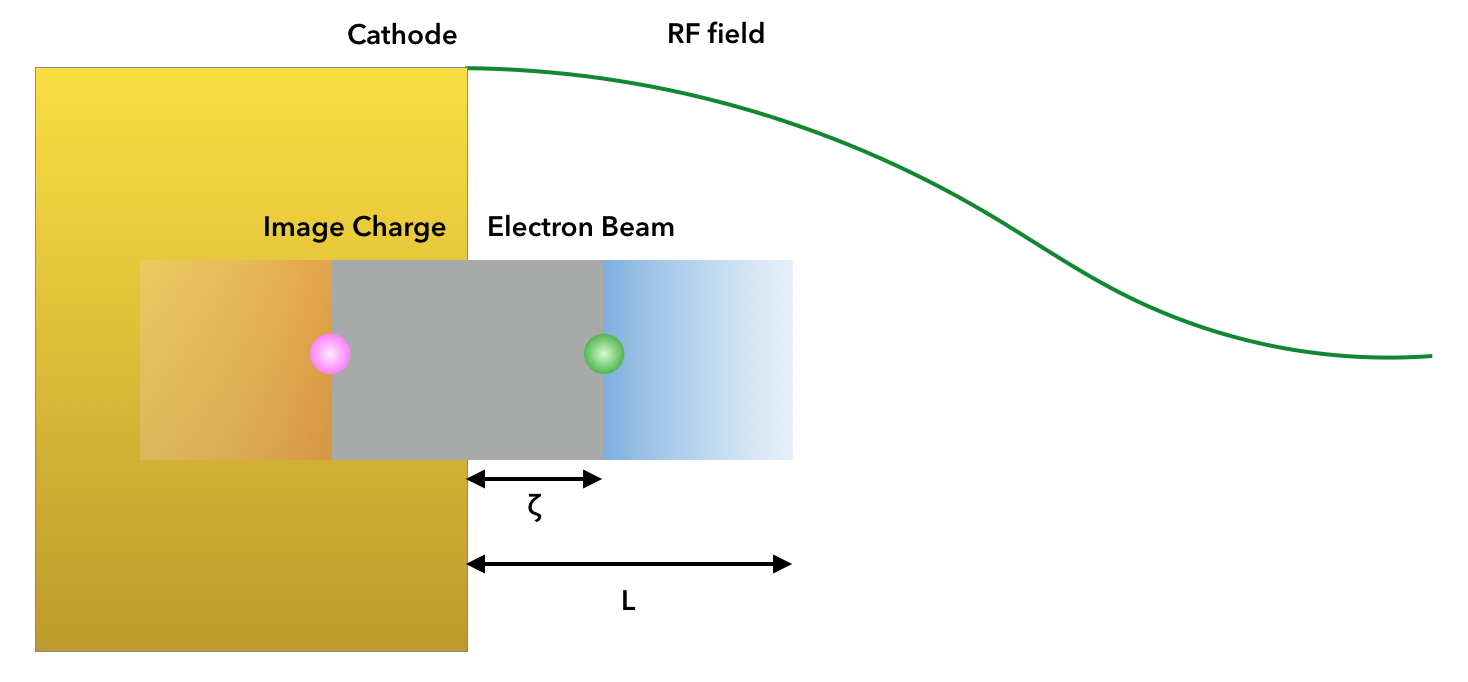
\includegraphics[width=0.9\textwidth]{schottky}
\caption{\label{fig:schottky-mod} 束团中某切片的发射过程示意图}
\end{figure}
如图中所示,在切片 $\zeta$ 从阴极表面出射到离开阴极一定距离的整个过程中,切片 $\zeta$ 以内(纵向相对位置 $< \zeta$)的电荷由于镜像电荷的存在,对切片 $\zeta$ 的作用为零;而切片 $\zeta$ 以外的电荷 $q$ 由于镜像电荷的存在,对切片 $\zeta$ 的作用会加强为两倍。同时考虑引出电场 $E_0$ 以及该切片中电子自身的镜像电荷力,有该切片中电子在发射过程中所感受到的总场强为:
\begin{equation}
-\frac{\partial\phi}{\partial z} = eE_0-e\frac{q}{\varepsilon_0 S}-\frac{e^2}{4\pi\varepsilon_0(2z)^2}
\end{equation}
注意扁平束情形下,空间电荷力对切片 $\zeta$ 的作用力在发射过程中可近似认为不变。上式与标准的单电子发射肖特基模型非常类似,仅需要将标准肖特基模型中的外场 $E_0$ 置换为 $E_0-q/\varepsilon_0S$ 即可,因此切片 $\zeta$ 中电子感受到的有效逸出功为:
\begin{equation}
\phi_{\text{eff}} = \phi_{w} - e\sqrt{\frac{e\big(E_0-(1-\zeta/L)\cdot Q/\varepsilon_0S\big)}{4\pi\varepsilon_0}}
\end{equation}
其中 $Q$ 为束团的总电荷量。各场对逸出功的贡献随切片离开阴极距离 $z$ 的变化如图 \ref{fig:schottky-mod} 所示。
\begin{figure}[htbp]
\centering
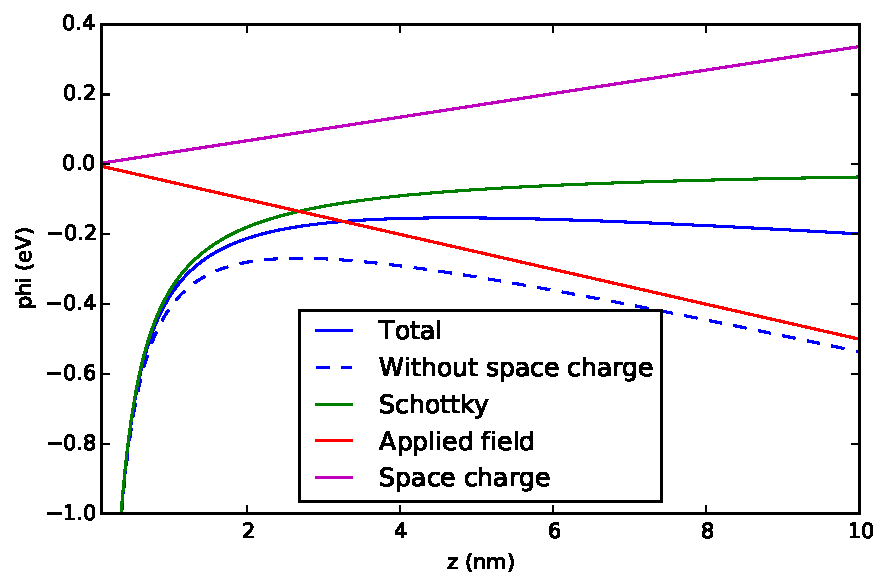
\includegraphics[width=0.6\textwidth]{schottky-mod}
\caption{\label{fig:schottky-mod} 考虑了空间电荷修正的肖特基效应示意图。}
\end{figure}

\subsubsection{考虑了切片发射度差异的束团热发射度}
如第三章所述,计算阴极上热发射度时可忽略动量分布与横向位置间的关系,因此依据统计发射度定义,第 i 个切片的发射度可写做:
\begin{eqnarray*}
\varepsilon_i^2 &=& \sigma_x^2\cdot\langle p_{x,i}^2\rangle \\
&=& \sigma_x^2\cdot\frac{\hbar\omega-\phi_w+e\sqrt{\frac{e\left(E_0-\frac{q_i}{\varepsilon_0 S}\right)}{4\pi\varepsilon_0}}}{3mc^2}
\end{eqnarray*}
这里假定激光纵向均匀分布,因此对于所有切片,其横向 rms 尺寸 $\sigma_{x,i}$ 都相等,等于激光的 $\sigma_{x}$;式中 $q_i$ 为指标大于 i 的切片的电荷量之和。

束团的总发射度为:
\[
\varepsilon^2 = \sigma_x^2\cdot\langle p_{x}^2\rangle
\]
因此有:
\begin{eqnarray}
\varepsilon^2 &=& \sigma_x^2\cdot\frac{\sum\limits_i Q_i\langle p_{x,i}^2\rangle}{\sum\limits_iQ_i} \label{eq:tot-emit-orig}\\
&=& \sigma_x^2\cdot\dfrac{\displaystyle\int_0^{Q}dq\frac{\hbar\omega-\phi_w+e\sqrt{\frac{e\left(E_0-\frac{q}{\varepsilon_0 S}\right)}{4\pi\varepsilon_0}}}{3mc^2}}{\displaystyle\int_0^{Q}dq}\nonumber\\
&=&\sigma_x^2\cdot\frac{\hbar\omega-\phi_w+e\sqrt{\frac{e}{4\pi\varepsilon_0}}\cdot\frac{2}{3}\frac{\varepsilon_0 S}{Q}\left(\sqrt{E_0}^3-\sqrt{E_0-\frac{Q}{\varepsilon_0 S}}^3\right)}{3mc^2}
\label{eq:tot-emit}
\end{eqnarray}
其中 $Q_i$ 为第 i 个切片的电荷量。注意上式化求和为积分一步做了变量代换 $Q-q \to q$,其中 $Q$ 为总电荷量,$q$ 为切片 $\zeta$ 以内的全部切片电荷量之和。

考虑空间电荷限发射($E_0=E_{SC}$)情形,由式 \ref{eq:tot-emit} 可知:
\begin{equation}
\varepsilon = \sigma_x\cdot\sqrt{\frac{\hbar\omega-\phi_w+e\sqrt{\frac{e\cdot\frac{4}{9}E_0}{4\pi\varepsilon_0}}}{3mc^2}}
\end{equation}
也即在空间电荷限发射情形下,发射束团的总发射度相当于不考虑切片空间电荷力时,阴极表面电场强度为 $E_0^*$ 的切片发射度,其中 $E_0^*$ 满足:
\begin{equation}
E_0^*=\frac{4}{9}E_0
\end{equation}
上式启发我们对式 \ref{eq:tot-emit} 进行一定的近似:
\begin{equation}
\varepsilon \approx \sigma_x\cdot\sqrt{\frac{\hbar\omega-\phi_w+e\sqrt{\frac{e\left(E_0-\frac{5}{9}\frac{Q}{\varepsilon_0 S}\right)}{4\pi\varepsilon_0}}}{3mc^2}}
\label{eq:tot-emit-approx}
\end{equation}
近似效果如图 \ref{fig:emit-mod} 所示。

\begin{figure}[htbp]
\centering
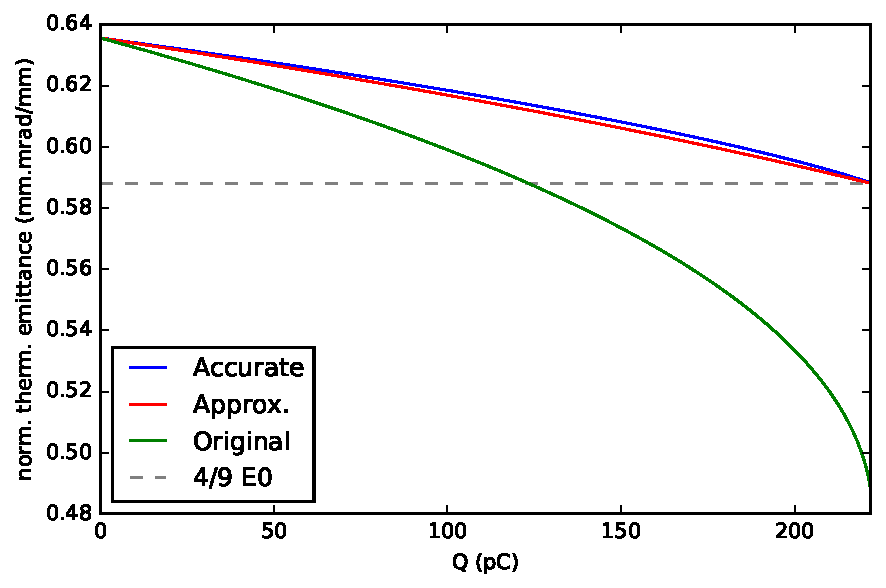
\includegraphics[width=0.6\textwidth]{emit-mod}
\caption{\label{fig:emit-mod} 修正前后的束团归一化发射度随发射电荷量的变化。}
\end{figure}

图 \ref{fig:emit-mod} 给出在 \SI{50}{MV/m} 的引出电场下的铜阴极表面束团热发射度随发射电荷量的变化。图中蓝色曲线对应式 \ref{eq:tot-emit},是精确的束团归一化发射度;红色曲线对应式 \ref{eq:tot-emit-approx},是近似的束团归一化发射度;绿色曲线对应式 \ref{eq:tot-emit-orig},是不考虑切片空间电荷力差异的束团归一化发射度;灰色虚线对应原始束团发射度公式 \ref{eq:tot-emit-none} 中代入 $4/9\cdot E_0$ 的束团归一化发射度。可以看到,精确解和近似解均在空间电荷限发射(对于 \SI{50}{MV/m} 的引出场强,铜阴极的空间电荷限发射对应电荷量约为 222\,pC)情形下收敛到灰色虚线。不考虑束流切片空间电荷力差异的束团发射度则与真实情况差距较大(且始终较真实情况偏小),在空间电荷限发射情形下,相对偏差约 20\%。图 \ref{fig:emit-mod} 还表明,当不考虑空间电荷力时(即发射电荷量为 0),各公式给出的归一化发射度均相等,这也是意料之中的结果。

\subsubsection{扁平束的极限热发射度计算}
上一节我们给出了一个近似效果较好的束团热发射度公式 \ref{eq:tot-emit-approx},下面就利用该式进行扁平束极限热发射度的估计。

依然采用前几节的模型,即激光横向圆均匀分布,纵向均匀分布;阴极材料为铜,光电发射方式为体发射。我们固定阴极表面场强 $E_0$,考察在该场强下阴极的极限热发射度。设激光半径为 $r$,那么 $\sigma_x = r/2$,结合式 \ref{eq:sc-limit},代入式 \ref{eq:tot-emit-approx},有:
\begin{equation}
\varepsilon \ge \frac{r}{2}\cdot\sqrt{\frac{\hbar\omega-\phi_w+e\sqrt{\frac{e\cdot\frac{4}{9}E_0}{4\pi\varepsilon_0}}}{3mc^2}} \ge \frac{1}{2}\cdot\sqrt{\frac{Q}{\varepsilon_0\pi E_0}}\cdot\sqrt{\frac{\hbar\omega-\phi_w+e\sqrt{\frac{e\cdot\frac{4}{9}E_0}{4\pi\varepsilon_0}}}{3mc^2}}
\end{equation}
上式中已不含可变参数(电荷量 $Q$ 是指定的,$E_0$ 也固定),因此扁平束的极限热发射度为:
\begin{equation}
\varepsilon_{\min} = \frac{1}{2\sqrt{3mc^2\varepsilon_0\pi}}\cdot\sqrt{Q}\cdot\sqrt{\frac{\hbar\omega-\phi_w}{E_0}+\frac{1}{3}e\sqrt{\frac{e}{\pi\varepsilon_0}}\cdot\frac{1}{\sqrt{E_0}}}
\label{eq:min-emit-pancake}
\end{equation}
取到极限热发射度的条件为空间电荷限发射($E_{SC}=E_0$)。

\subsubsection{扁平束极限热发射度的讨论}
式 \ref{eq:min-emit-pancake} 给出了扁平束的极限热发射度,观察该式,就得到以下两个基本结论:
\begin{itemize}
\item 极限发射度与发射电荷量 $Q$ 的平方根成正比,即:
\begin{equation}
\varepsilon_{\min} \propto \sqrt{Q}
\end{equation}
\item 若 $\hbar\omega-\phi_w \ge 0$,阴极表面场强越大,极限发射度越小
\end{itemize}
对于铜阴极而言,若采用 266\,nm 激光,则$\hbar\omega-\phi_w = \SI{4.66}{eV}-\SI{4.31}{eV} = \SI{0.35}{eV}$,显然满足第二条,因此想要降低铜阴极的初始热发射度,就必须提高表面场强 $E_0$;同时提高表面场强 $E_0$ 也有助于快速将束流加速到接近光速,抑制低能阶段的空间电荷力对热发射度的破坏。

将场强 $E_0=\SI{50}{MV/m}$,电荷量 $Q=\SI{200}{pC}$ 代入式 \ref{eq:min-emit-pancake},就得到铜阴极在典型条件下的极限热发射度:
\begin{equation}
\varepsilon_{\min, \text{Cu}} = \SI{0.11}{mm\cdot mrad}
\end{equation}
此时对应的激光半径 $r=\SI{379.2}{\mu\meter}$。式 \ref{eq:min-emit-pancake} 可以化成一个对工程更友好的形式:
\begin{equation}
\varepsilon_{\min} = \sqrt{Q}\cdot\sqrt{\frac{5.863(\hbar\omega-\phi_w)}{E_0}+\frac{0.1483}{\sqrt{E_0}}}
\label{eq:min-emit-pancake-eig}
\end{equation}
其中 $\varepsilon_{\min}$ 的单位为 mm$\cdot$mrad,$Q$ 的单位为 nC,$E_0$ 的单位为 MV/m,$\hbar\omega$ 和 $\phi_w$ 的单位为 eV。

上面讨论了 $\hbar\omega-\phi_w \ge 0$ 的情况,$\hbar\omega-\phi_w < 0$ 时情况更加复杂,表面上 $\varepsilon_{\min}$ 不再是 $E_0$ 的单调减函数,而是与 $1/\sqrt{E_0}$ 构成椭圆关系;但由更细致的分析可知,该情形下不可能达到空间电荷限发射条件(因为在空间电荷限达成之前光电子发射就已经由于光电子无法穿过表面势垒而截止了),因而其极限发射度不能再由式 \ref{eq:min-emit-pancake} 描述。具体分析这里就暂不展开了。

\subsection{笔形束的极限热发射度}
笔形束的极限热发射度分析过程与扁平束的非常类似,唯一的不同在于空间电荷限的估算,对于纵横比远大于 1 的笔形束来说,纵向空间电荷场不能再用式 \ref{eq:e-sc-pancake} 来近似。想要给出笔形束中某切片在发射时所感受到的场的(近似)解析表达式较为困难,但如果仅仅想估计笔形束的极限发射度,可以采用如下的想法绕开数学上的困难。

\subsubsection{笔形束的阴极饱和电流}
依然将长束团划分为若干薄切片,考虑某距离阴极为 $z$ 的切片对阴极表面中心的电场,就有(包含镜像电荷效应):
\begin{equation}
E_{SC}(z) = \frac{\sigma}{\varepsilon_0}\left(1-\frac{z}{\sqrt{z^2+r^2}}\right)
\label{eq:slice-sc}
\end{equation}
其中 $r$ 为该切片半径,$\sigma$ 为该切片的面电荷密度。从上面的形式看到,若 $z/r \ll 1$,$E_{SC}(z)\approx \sigma/\varepsilon_0$,即趋向于扁平束中的空间电荷场表达式;若 $z/r \gg 1$,$E_{SC}(z)\approx q/2\pi\varepsilon_0z^2$,其中 $q = \pi r^2 \sigma$ 为该切片电荷量,即趋于点电荷与镜像点电荷对阴极表面的作用。图 \ref{fig:slice-sc} 给出了式 \ref{eq:slice-sc} 中电场随距离 $z$ 的变化。
\begin{figure}[htbp]
\centering
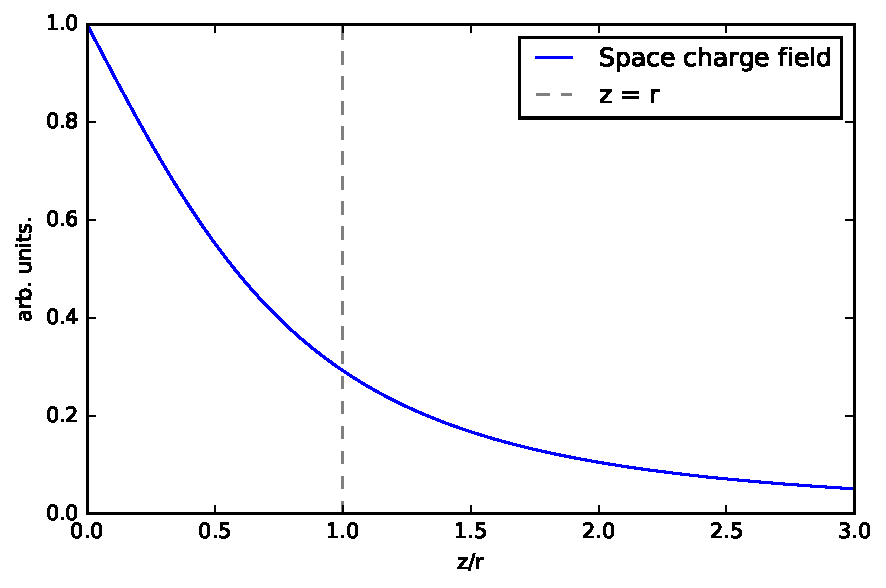
\includegraphics[width=0.6\textwidth]{slice-sc}
\caption{\label{fig:slice-sc} 长束团切片在阴极上的空间电荷场}
\end{figure}
图中可见,当距离 $z$ 与切片半径相等时,该切片对阴极的作用已经相当弱,由此引出了有效作用长度 $z_{\text{eff}}$ 的概念:即只有距离阴极 $z_{\text{eff}}=\eta r$ 以内的切片才会对阴极表面空间电荷场有贡献。将阴极表面有效距离内的束流看做稳定饱和束流(令阴极表面总电场为 0),那么利用 Child-Langmuir 定律,有饱和电流:
\begin{equation}
I_{\text{sat}} = \frac{1}{\sqrt{\eta}}I_0\frac{\sqrt{2}}{9}\left(\frac{eE_0r}{mc^2}\right)^{\frac{3}{2}}
\end{equation}
其中 $I_0=4\pi\varepsilon_0mc^3/e\approx\SI{17}{kA}$ 为 Alfven 电流。模拟证明,在相当大的范围里 $\eta\approx 1$,因此饱和电流可近似为:
\begin{equation}
I_{\text{sat}} \approx I_0\frac{\sqrt{2}}{9}\left(\frac{eE_0r}{mc^2}\right)^{\frac{3}{2}}
\label{eq:sat-I}
\end{equation}

\subsubsection{笔形束的极限热发射度估计}
现在估计笔形束的极限热发射度。由式 \ref{eq:tot-emit-orig} 可知,束团的总发射度为各切片发射度的均方根,而由上节的分析知道,当束团发射长度长于激光横向尺寸时,阴极表面上的空间电荷场强度几乎不再变化;而束团的纵向长度又远远大于横向尺寸,因此束团中绝大多数切片的发射度都相等,等于阴极表面空间电荷场饱和时对应的切片发射度:
\begin{equation}
\varepsilon = \varepsilon_{\text{slice, sat}}
\end{equation}
另一方面,越接近空间电荷限发射,阴极上的饱和空间电荷场越大,那么由有效逸出功修正一节可知,其对应的有效逸出功也就越大,进而饱和切片发射度越小,最小值即阴极表面总电场为 0 时的切片发射度。由此,想达到极限发射度,其条件与扁平束一样,就是空间电荷限发射。注意,为保证空间电荷限发射可达到,这里假定了 $\hbar\omega-\phi_w \ge 0$。

由此,结合饱和电流式 \ref{eq:sat-I},我们有笔形束的极限热发射度估计:
\begin{equation}
\varepsilon \ge \frac{r}{2}\cdot\sqrt{\frac{\hbar\omega-\phi_w}{3mc^2}} \ge \frac{mc^2}{2eE_0}\left(\frac{9Q}{\sqrt{2}I_0\tau}\right)^{\frac{2}{3}}\cdot\sqrt{\frac{\hbar\omega-\phi_w}{3mc^2}}
\end{equation}
其中 $\tau$ 为阴极上的束流脉宽。于是:
\begin{equation}
\varepsilon_{\min} = \left(\frac{9}{16\pi\varepsilon_0}\sqrt{\frac{m}{e}}\right)^{\frac{2}{3}}\cdot\sqrt{\frac{\hbar\omega-\phi_w}{3mc^2}}\cdot\left(\frac{Q}{\tau}\right)^{\frac{2}{3}}\frac{1}{E_0}
\label{eq:min-emit-cigar}
\end{equation}

\subsubsection{笔形束极限热发射度的讨论}
式 \ref{eq:min-emit-cigar} 给出了笔形束的极限热发射度,观察该式,就得到以下两个基本结论:
\begin{itemize}
\item 极限发射度与发射电流 $Q/\tau$ 的三分之二次方成正比,即:
\begin{equation}
\varepsilon_{\min} \propto (Q/\tau)^{\frac{2}{3}}
\end{equation}
\item 极限发射度与阴极表面场强 $E_0$ 成反比,即:
\begin{equation}
\varepsilon_{\min} \propto 1/E_0
\end{equation}
\end{itemize}
第二条结论说明,与扁平束的情况相同,想获得更低的热发射度就要尽可能地提高表面场强。而第一条结论与扁平束的情形相当不同:极限热发射度中出现了阴极上的束流脉宽 $\tau$,这意味着在相同电荷量下,为获得更低的极限热发射度,需要拉长阴极上的束长!

然而阴极表面束流脉宽并不能无限制地拉长,因为过长的束流会占有相当的微波场相位,进而会引入高阶 RF 效应,导致在后续的光阴极枪及注入器中传输时发射度发生不可逆增长。

代入一组典型参数(铜阴极,场强 $E_0=\SI{50}{MV/m}$,电荷量 $Q=\SI{200}{pC}$,激光脉宽 $\tau=\SI{10}{ps}$)到式 \ref{eq:min-emit-cigar},就有此情形下的极限热发射度:
\begin{equation}
\varepsilon_{\min, \text{Cu}} = \SI{0.09}{mm\cdot mrad}
\end{equation}
此时对应的激光半径 $r=\SI{390.4}{\mu\meter}$。式 \ref{eq:min-emit-cigar} 可以化成一个对工程更友好的形式:
\begin{equation}
\varepsilon_{\min} = 1.070\sqrt{\hbar\omega-\phi_w}\cdot\left(\frac{Q}{\tau}\right)^{\frac{2}{3}}\frac{1}{E_0}
\label{eq:min-emit-cigar-eig}
\end{equation}
其中 $\varepsilon_{\min}$ 的单位为 mm$\cdot$mrad,$Q$ 的单位为 pC,$\tau$ 的单位为 ps,$E_0$ 的单位为 MV/m,$\hbar\omega$ 和 $\phi_w$ 的单位为 eV。

\subsection{阴极热发射度与注入器出口处的发射度}
前两节我们讨论了阴极表面的两种发射模式:扁平束发射和笔形束发射。比较二者典型参数下的极限热发射度,可以看到笔形束的热发射度要优于扁平束的热发射度,一些模拟和实验探索也证明将束团初始长度拉长有助于降低光阴极注入器出口处的发射度。然而,阴极上的热发射度与注入器出口处的束流发射度一般并不相等。阴极上产生的束团在后续的传输过程中,会受到束团自身非线性空间电荷力的作用(束团分布只要不是 KV 分布就一定存在非线性空间电荷力);由于束团有一定长度占一定的射频相位,因此射频场的高阶成分也会对束团产生非线性射频场的作用;另外,由于束团具有一定能散,注入器中的各束流操纵元件,例如发射度补偿螺线管线圈,四极磁铁等会对束团产生色散效应。以上各因素都会导致束团初始热发射度有不同程度的增大,因此优化注入器发射度时,不能仅仅将光阴极上的热发射度优化到最小,还要考虑该热发射度是否能够较好地保持到注入器出口,这就要对初始激光参数与注入器各元件的参数进行统一的优化。接下来的章节,先引入双频光阴极微波电子枪的概念,随后应用遗传算法对双频电子枪注入器进行多变量多目标优化,以求达到注入器出口处发射度的较优值。

\section{双频光阴极微波电子枪}
经过多年的模拟和实验探索,目前光阴极注入器出口处的束团横向亮度已经趋近于光阴极表面的最大束流亮度。想进一步提高束流亮度,可以提高阴极表面电场强度,降低光电发射时的电子剩余动能,或者将激光的尺寸从扁平状改变为细长状(笔形束)。光电发射时采用笔形束的基本原理是牺牲光电流的峰值流强,降低空间电荷效应,抑制发射度增长。因此如果采用笔形束方案,为保持光阴极注入器出口处流强足够(一般 FEL 的应用对注入器出口处的流强要求为 30\,A 左右),必须要使用聚束腔(buncher)。然而,由于笔形束的纵向尺寸较大,占有一定的微波相位,RF 发射度就会增长,进而束团的纵向分布在聚束后就会变得高度不对称,这样的束流对于 XFEL 等应用其出光品质就会降低。

为了降低 RF 发射度增长以及减小束团纵向分布不对称性,空间叠加型光阴极电子枪的概念应运而生。典型的空间叠加型光阴极电子枪结构见图 \ref{fig:overlapgun}。

\begin{figure}[htbp]
\centering
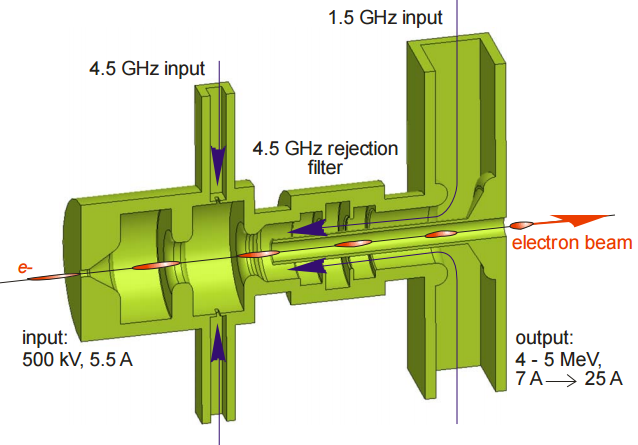
\includegraphics[width=0.6\textwidth]{overlapgun}
\caption{\label{fig:overlapgun} PSI 设计的空间叠加型光阴极电子枪结构图。}
\end{figure}

其原理为:将基模和高阶模(一般是三阶模)叠加在同一个腔体内,那么在某一段 RF 相位区间就会形成一段线性的微波场,如图 \ref{fig:linearfield} 所示。工作时将电子束置于该相位区间,则原来的微波场造成的二阶 RF 效应就被补偿,电子束从始至终处于一个线性场区,其引入的能量调制为线性,从而实现均匀的压缩,即在保持发射度以及峰值流强的情况下,使电子束的纵向分布也尽量均匀,提高后续的出光效率。

\begin{figure}[htbp]
\centering
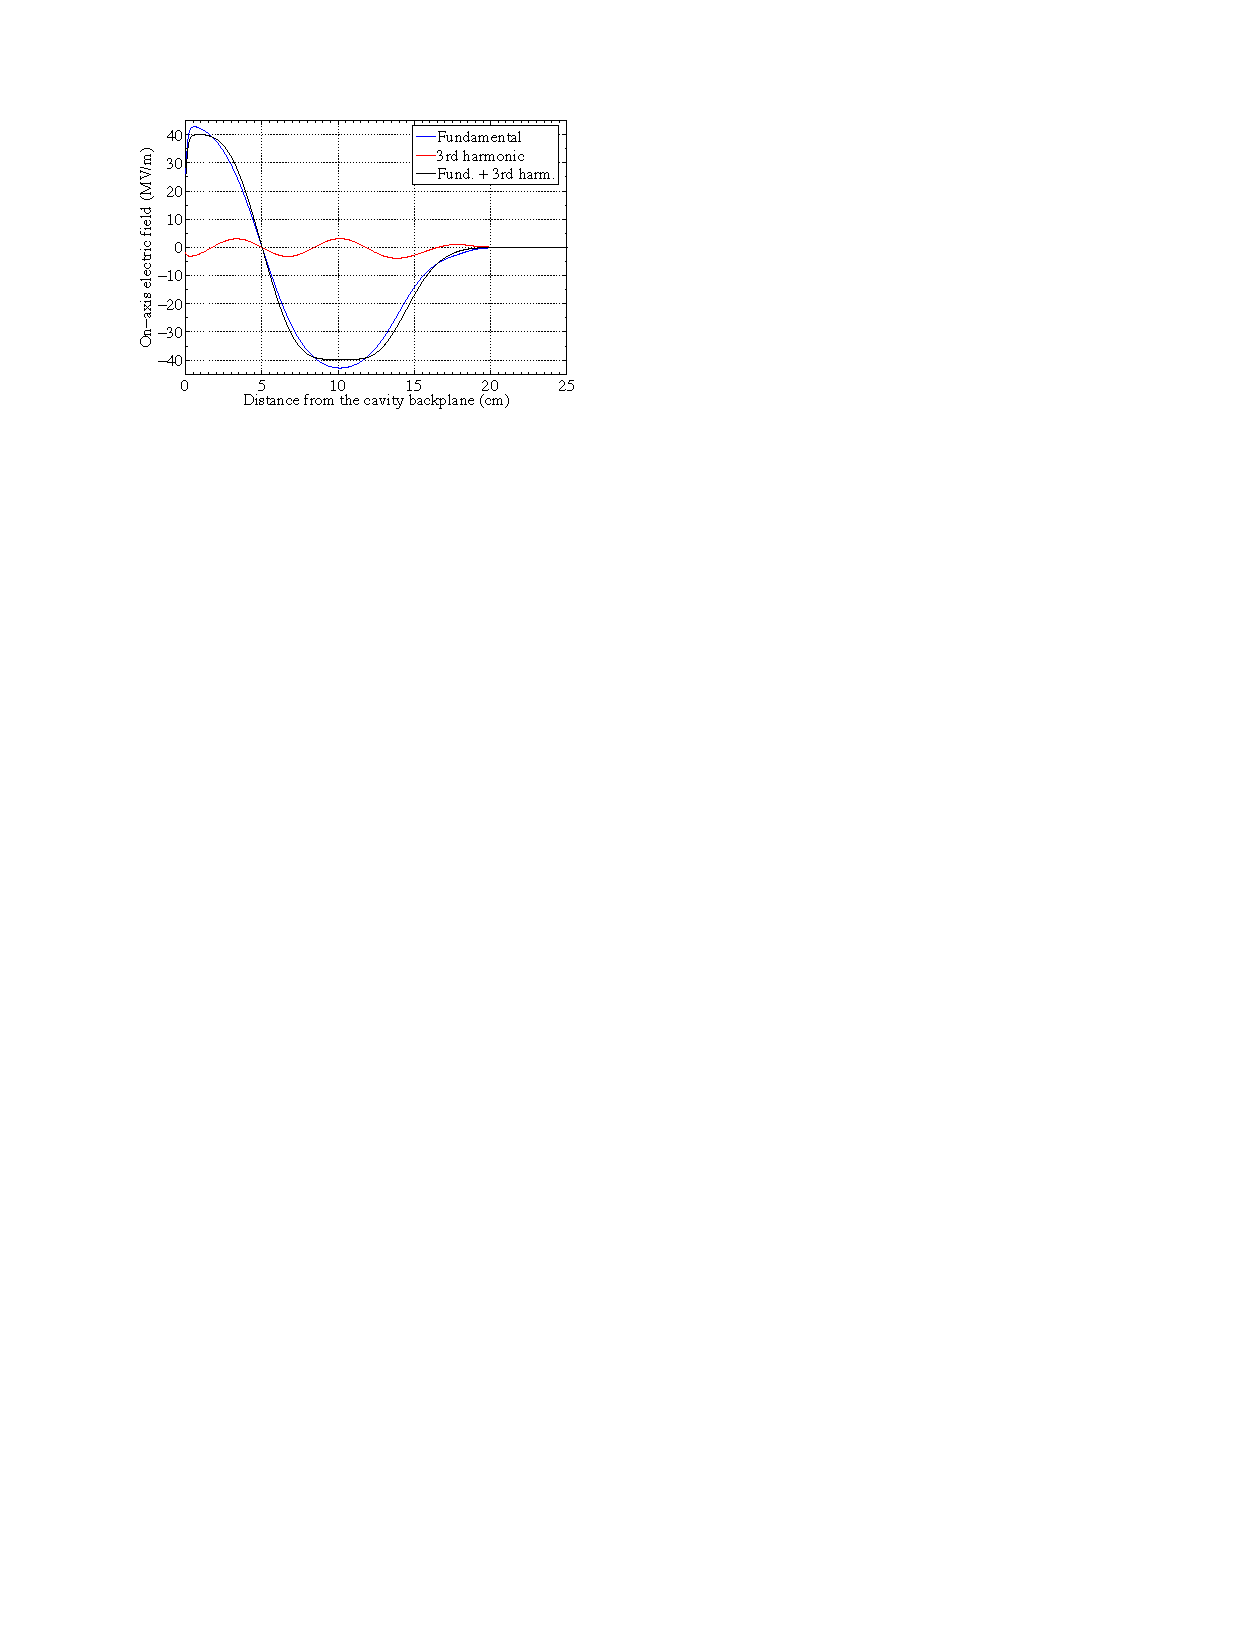
\includegraphics[width=0.6\textwidth]{overlap}
\caption{\label{fig:linearfield} 空间叠加型光阴极电子枪中的微波场。}
\end{figure}

尽管空间叠加型电子枪的原理已经由束流动力学模拟所验证,想真正实现这个想法却是很困难的:一把空间叠加型电子枪需要两个耦合器和一个过滤器,并且要在同一个腔中同时调谐和调平基模和高阶模(HOM)两个模式,其工程难度是巨大的。受此思想启发,我们提出了一种不同的路线来实现双频电子枪,即将两个 RF 模式在空间上分离开,分别将它们放在基模腔和高阶模腔中,并将基模腔和高阶模腔紧凑地组合起来,就形成了空间分离双频电子枪。

实际设计中,我们将一个 BNL 型 1.6 cell S 波段电子枪和一个高阶模腔集成在一起,初始束团的纵向尺寸先被拉长,抑制了空间电荷力发射度的增长,随后在束流经过高阶模腔时进行聚束,这样就可以在注入器出口处获得较高的峰值流强。由于相同的电荷量下,较长束团对应的横向尺寸较小,因此此举也可减小阴极表面初始热发射度。空间分离双频电子枪中的高频腔也同时可对束流纵向相空间进行线性化,从而补偿掉微波场的二阶效应,从而可在注入器出口形成对称束流,这对电子束团的后续应用有很大好处。

\section{空间分离双频电子枪的腔型设计}
我们选择了 S 波段的四阶模 X 波段作为高频腔的工作波段,并利用 Superfish 做电磁场模拟以进行腔结构参数设计。在腔型尺寸设计中,主要考察了以下几个限制条件:1)基频腔和高频腔的工作模式频率要分别为 S 波段和 X 波段;2)S 波段模式的场要调平;3)X 波段模式渗透到 S 波段腔体的场不能太强。为了同时满足三个条件,选定了 S 波段半腔半径,S 波段整腔半径与 X 波段腔半径作为输入变量;两个模式的频率,S 波段模式场平为目标变量,对腔型进行优化。

X 波段模式的场渗透率(X 波段模式在 S 波段腔中最高场强与在 X 波段腔中最高场强之比)可以通过调节 X 波段高频腔的位置进行控制,且后续动力学模拟中可能对高频腔位置有反馈,因此腔型优化可能对于 X 波段高频腔的不同位置反复进行多次。鉴于此,我们借鉴梯度下降法的思想编写了腔型自动优化算法,实现对腔型的自动优化。

\subsection{腔型自动优化算法}
腔型自动优化算法的基本思想如下:假定我们的目标为 $\mathbf{y_t} = (y_{1,t}, y_{2,t}, y_{3,t})^T$,那么优化问题实质是找到使:
\begin{equation}
\label{eq:newton}
\mathbf{y_t} = f(\mathbf{x_t})
\end{equation}
成立的 $\mathbf{x_t}$,其中 $f$ 即系统对输入变量的响应函数,一般情况下具体形式未知(但是对于给定的输入,系统可以给出响应,例如任何一个动力学模拟的模拟结果对于束线的参数的响应函数就是这样的情形)。采用类似牛顿法求根的思想,若我们相信使得式 \ref{eq:newton} 成立的 $\mathbf{x_t}$ 一定存在,那么只要从输入变量初始值 $\mathbf{x} = (x_{1}, x_{2}, x_{3})^T$ 开始,求出该点处响应函数的值 $\mathbf{y} = (y_{1}, y_{2}, y_{3})^T$ 及梯度 $\mathbf{M}$(即雅可比矩阵):
\[
d\mathbf{y} = \mathbf{M}\cdot d\mathbf{x}
\]
及此时的目标差距 $\mathbf{\Delta} = \mathbf{y_t}-\mathbf{y} = (y_{1,t}-y_1, y_{2,t}-y_2, y_{3,t}-y_3)^T$,就可以求出预期的 $\mathbf{x_t^*}$:
\begin{equation}
\label{eq:delta}
\mathbf{x_t^*} = \mathbf{M}^{-1}\cdot\mathbf{\Delta}+\mathbf{x}
\end{equation}
由于一般动力学系统的响应函数并非线性,因此 $\mathbf{x_t^*}$ 一般不会是真解,但若响应函数 $f$ 性质较好,则式 \ref{eq:delta} 会给出一个距离真解更近的解;以该解作为新的输入变量,重复以上步骤,就获得一系列解 $\mathbf{x}, \mathbf{x_t^*}, \mathbf{x_t^{**}, \dots}$ 及对应的目标差距 $\mathbf{\Delta}, \mathbf{\Delta^*}, \mathbf{\Delta^{**}, \dots}$,随着迭代次数增加,解序列会逐渐趋近于真解 $\mathbf{x_t}$,目标差距序列会逐渐趋近于 $\mathbf{0}$。

实际优化中,我们采用下式而非式 \ref{eq:delta} 生成解序列:
\begin{equation}
\label{eq:delta2}
\mathbf{x_t^*} = \eta\mathbf{M}^{-1}\cdot\mathbf{\Delta}+\mathbf{x}
\end{equation}
其中 $\eta$ 为一个 0 到 1 之间的因子,与收敛速度相关。经过实验,我们最终采用 $\eta=1/2$ 进行优化求解。

能够应用以上算法的前提是:1)要保证解存在;2)输入变量与目标变量维数相同(维数可以更高,不限定是三维的)。第二点是保证雅可比矩阵是方阵,有可逆的可能性。因此在腔型优化中,采用了三输入变量,三目标变量的设置。

我们使用 Python 编程实现了上述算法。实现过程的重点是如何给出某点的雅可比矩阵,我们采用了下面的办法:首先计算输入变量 $\mathbf{x}$ 对应的输出 $\mathbf{y}$;随后对于输入变量的某一分量 $x_i$ 取增量 $dx_i$ 变为 $x_i^{\prime}$,计算输入变量为 $\mathbf{x}_i^{\prime} = (x_1, x_2,\dots,x_i^{\prime},\dots,x_n)^T$ 的响应 $\mathbf{y}_i^{\prime}$,也即仅将输入变量第 i 维取增量时的系统响应,那么雅可比矩阵就可写为:
\begin{equation}
\label{eq:jacob}
\mathbf{M} = \left(\frac{\mathbf{y}_1^{\prime}-\mathbf{y}}{dx_1}, \frac{\mathbf{y}_2^{\prime}-\mathbf{y}}{dx_2}, \dots, \frac{\mathbf{y}_n^{\prime}-\mathbf{y}}{dx_n}\right)
\end{equation}
对于本节中的腔型优化问题,可以估算迭代一次所需的模拟次数:对原始输入变量求输出需要一次模拟,生成雅可比矩阵需要三次模拟,因此一次迭代需要四次模拟。实际优化中,发现该优化算法的收敛速度极快,对于较好的初始输入值,达到精度要求或收敛(由于加工精度有限,模拟中各尺寸的精度到 10\,$\mu$m 量级,因此迭代进行到一定次数后新给出的输入变量由于四舍五入而保持与上一组输入变量相同,此时优化算法收敛,但给定的目标变量精度要求可能并未达到)只需要三次左右的迭代,因此一次完整优化只需要运行 12 次模拟,效率很高。

\subsection{腔型优化后的结构参数及场分布}
我们将 X 波段高频腔放在离 S 波段腔尽可能近(但保持场渗透率低于千分之一)的位置,应用自动优化算法,最终得到整体双频电子枪腔型及场分布见图 \ref{fig:field_sx}。S 波段腔型微波及结构参数见表 \ref{tab:geo_s},X 波段腔型微波及结构参数见表 \ref{tab:geo_x}。
\begin{figure}[htbp]
	\centering
	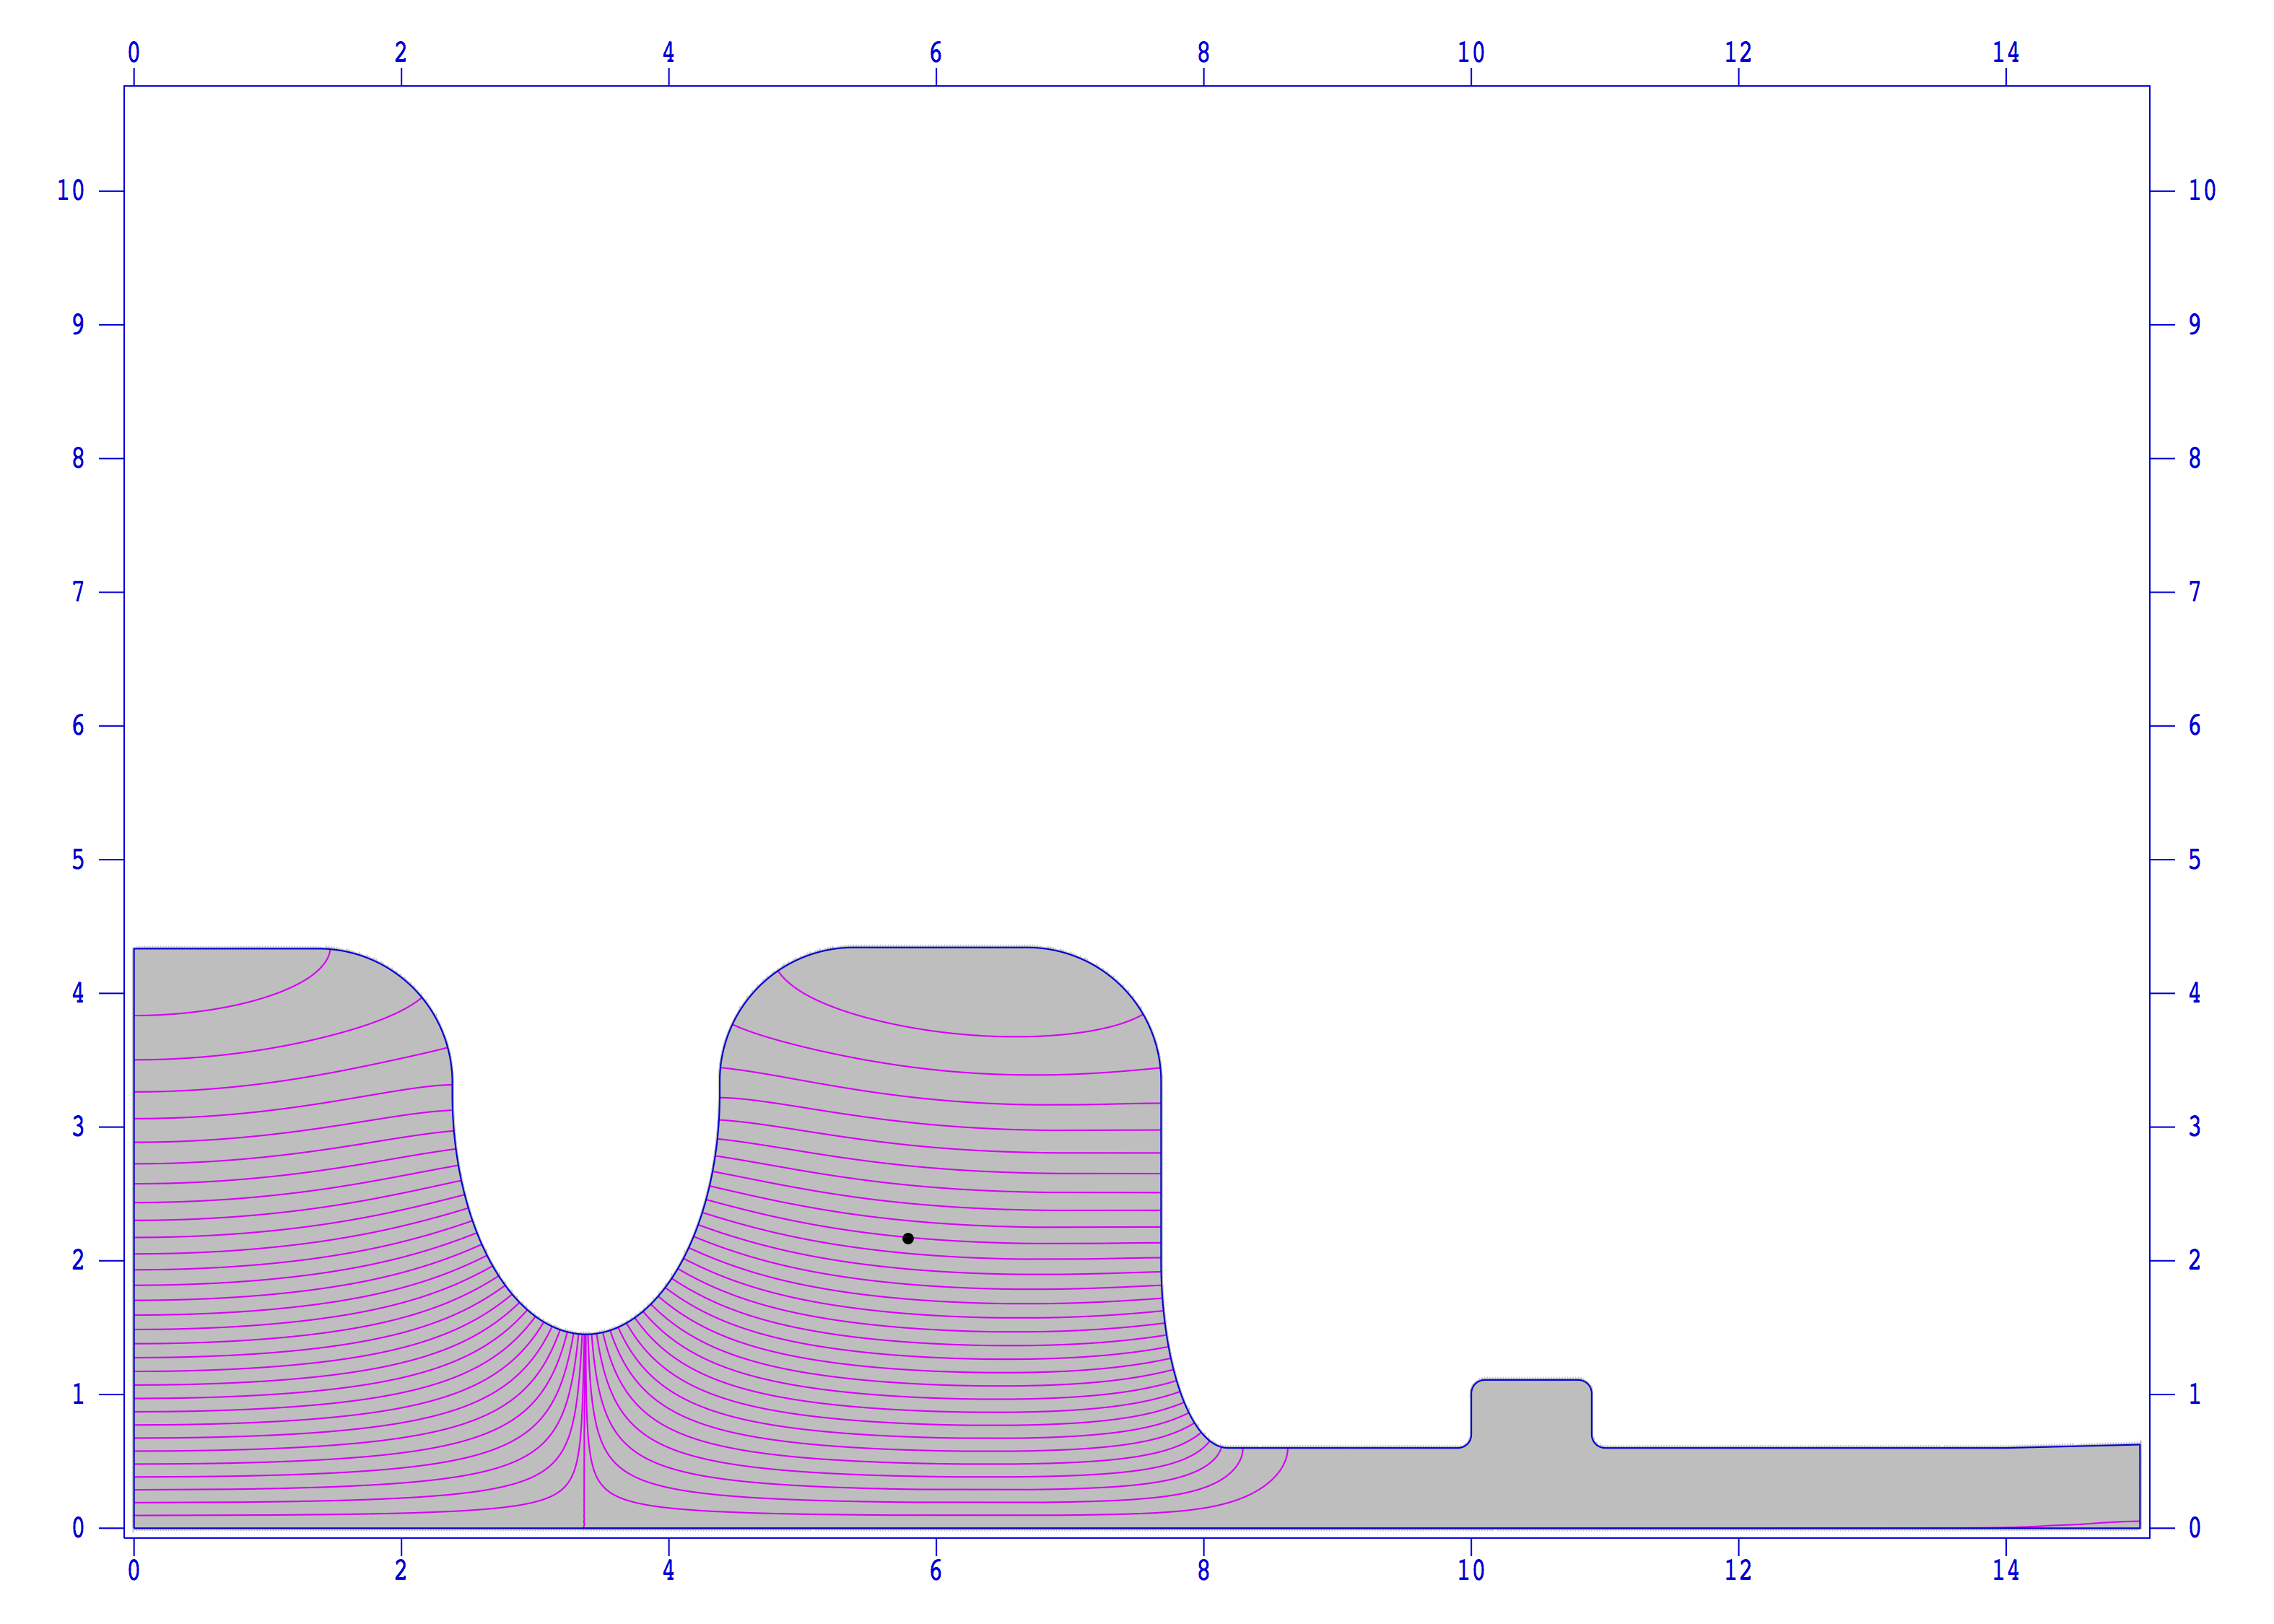
\includegraphics[width=0.45\textwidth]{field_s}
	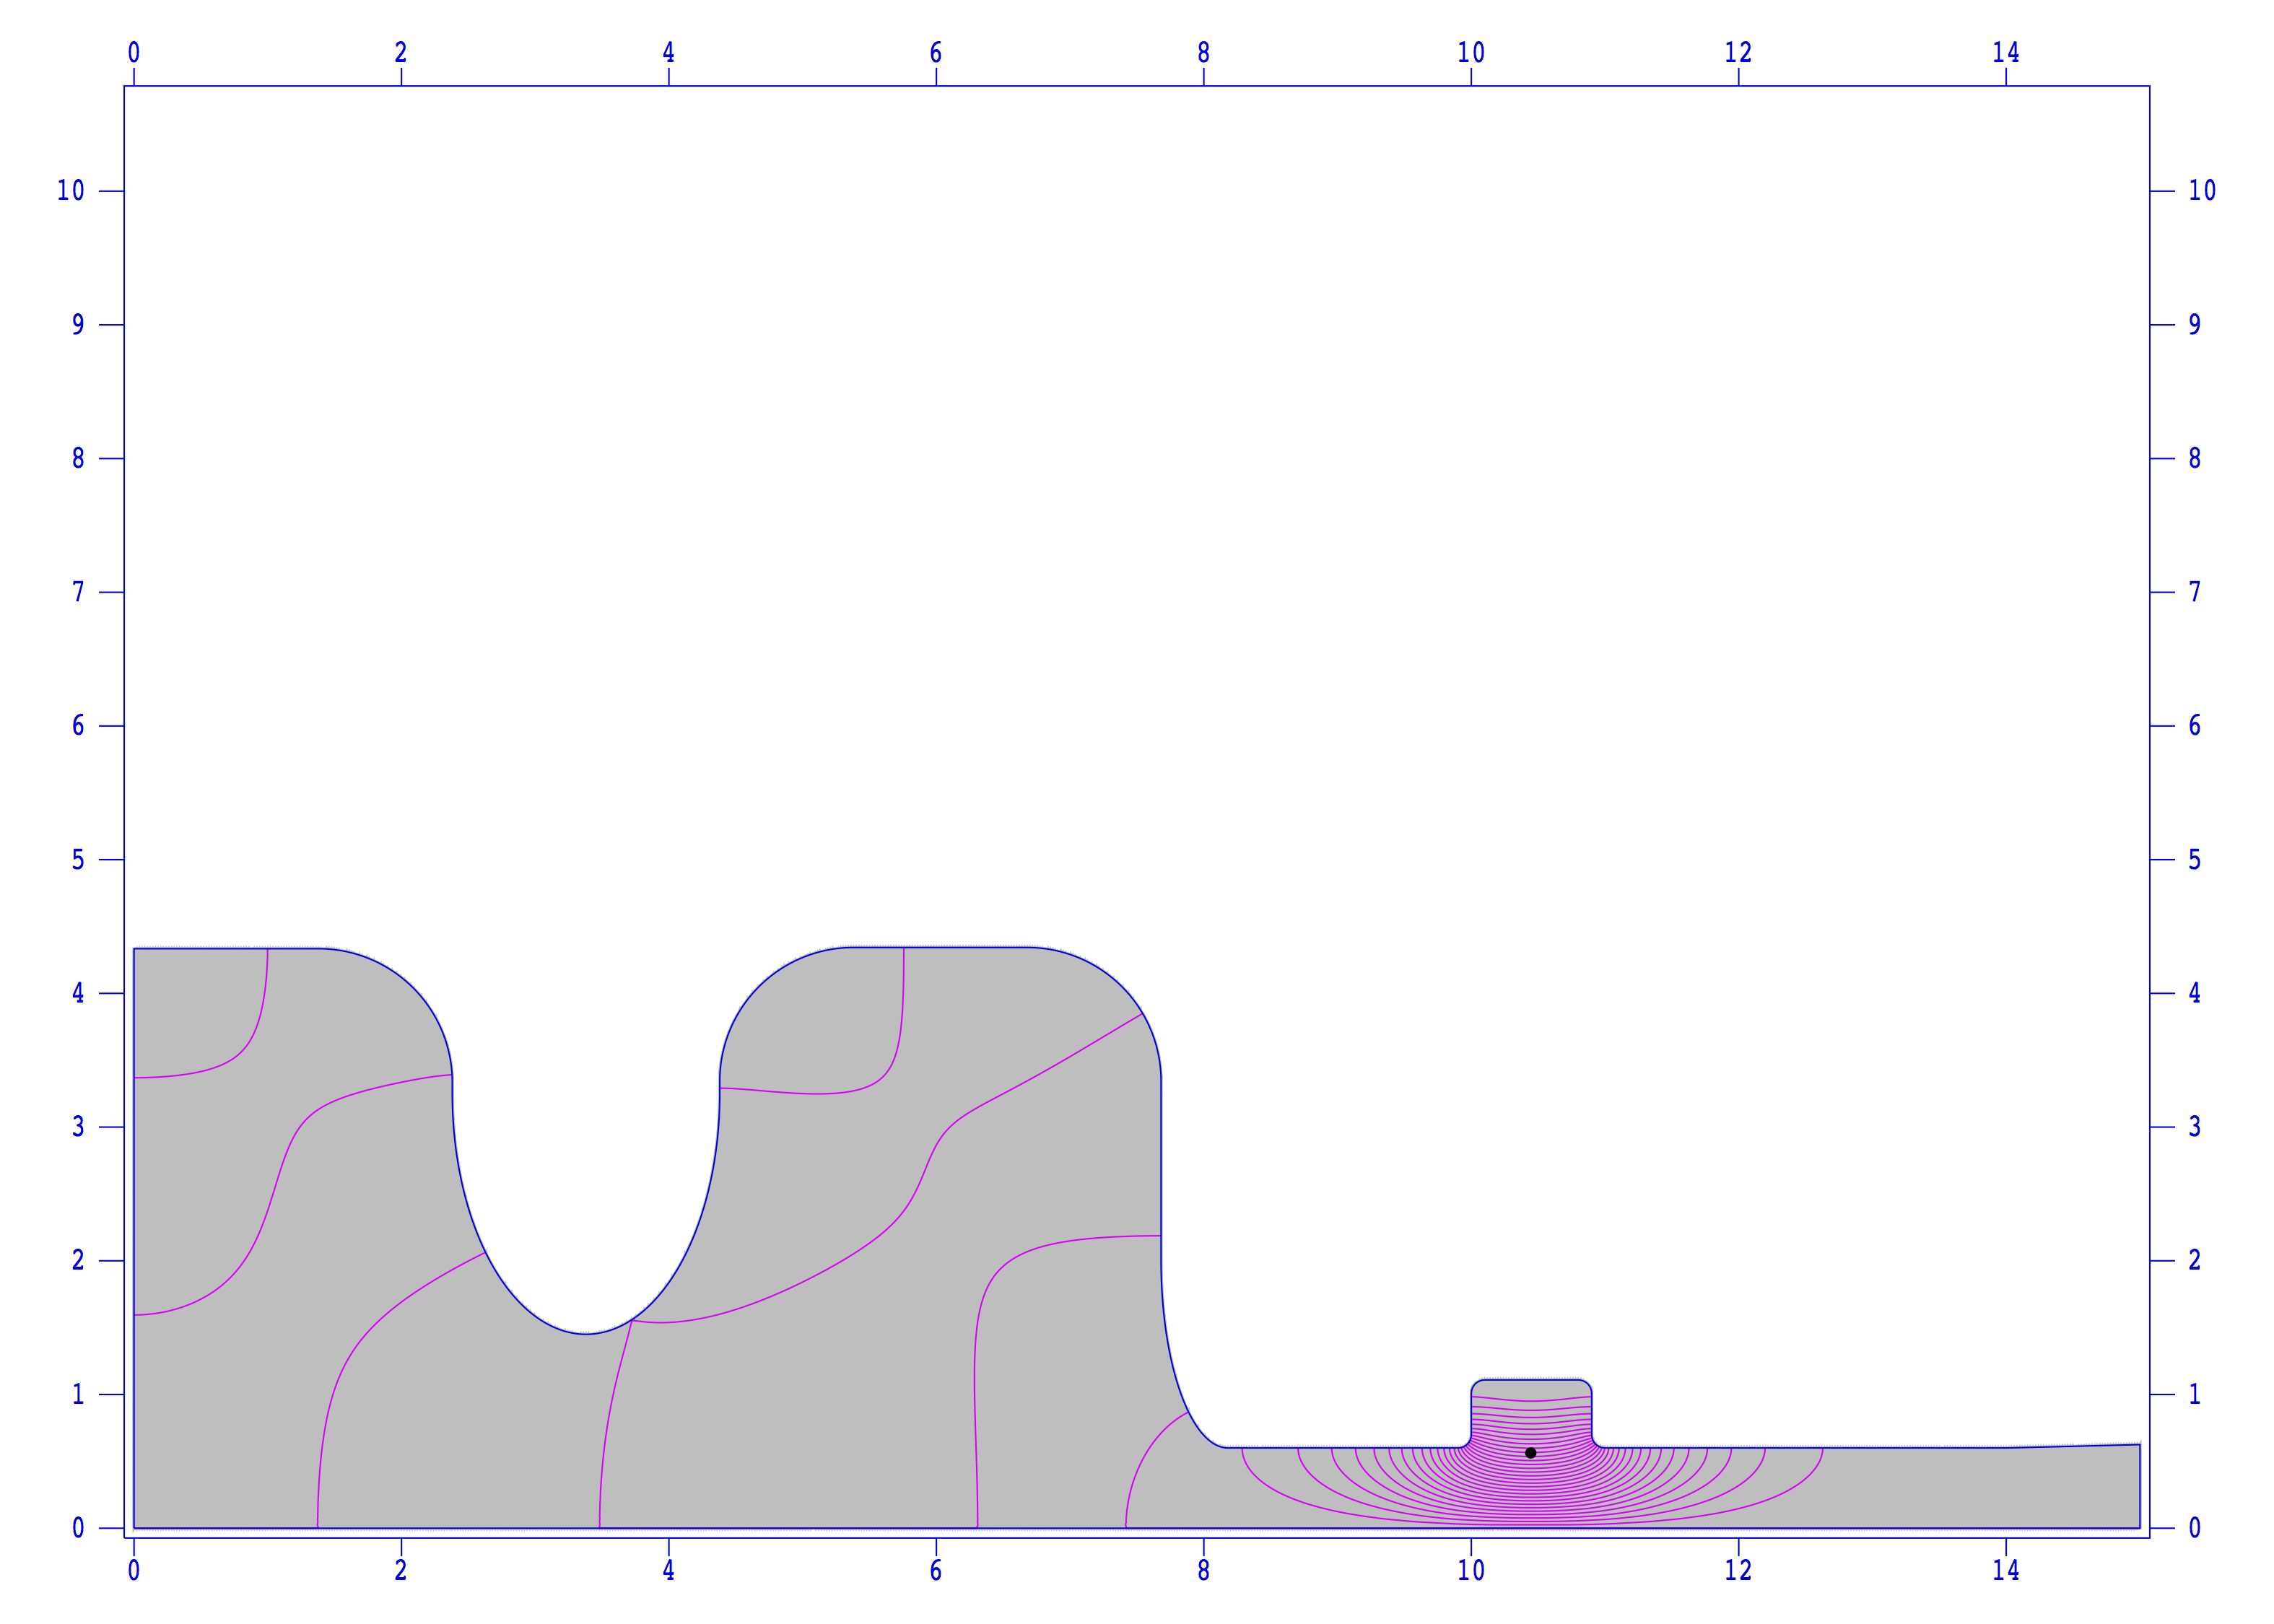
\includegraphics[width=0.45\textwidth]{field_x}
	\caption{
	双频电子枪中的电场分布。左图:S 波段基模电场分布;右图:X 波段高阶模电场分布。}
	\label{fig:field_sx}
\end{figure}

\begin{table}[htbp]
\centering
\caption{\label{tab:geo_s}
S 波段腔结构参数。}
\begin{tabular}{lll}
\toprule
参数 & 值 & 描述\\
\midrule
freq & \SI{2856.00}{MHz} & 微波频率  \\
flatness & 0.9996 & 场平  \\
\midrule
$l_h$ & \SI{3.38}{cm} & 半腔长度  \\
$r_h$ & \SI{4.3341}{cm} & 半腔半径  \\
$c_h$ & \SI{1}{cm} & 半腔倒角半径  \\
$j_h$ & \SI{1}{cm}, \SI{1.8}{cm} & 半腔盘片长、短轴 a、b \\
$l_f$ & \SI{4.8}{cm} & 整腔长度  \\
$r_f$ & \SI{4.3431}{cm} & 整腔半径  \\
$c_f$ & \SI{1}{cm} & 整腔倒角半径  \\
$j_{f, l}$ & \SI{1}{cm}, \SI{1.8}{cm} & 整腔左盘片长、短轴 a、b \\
$j_{f, r}$ & \SI{0.5}{cm}, \SI{1.4}{cm} & 整腔右盘片长、短轴 a、b \\
$r_{f, t}$ & \SI{1.45}{cm} & 束流管道半径  \\
\bottomrule
\end{tabular}
\end{table}

\begin{table}[htbp]
\centering
\caption{\label{tab:geo_x}
X 波段腔结构参数。}
\begin{tabular}{lll}
\toprule
参数 & 值 & 描述\\
\midrule
freq & \SI{11424.25}{MHz} & 微波频率  \\
penetration & $3.02\times10^{-4}$ & 场渗透率  \\
\midrule
$p$ & \SI{9.9}{cm} & 腔起始位置  \\
$l$ & \SI{1.1}{cm} & 腔长度  \\
$r$ & \SI{1.1088}{cm} & 腔半径  \\
$c$ & \SI{0.1}{cm} & 腔倒角半径  \\
$j$ & \SI{0.1}{cm} & 腔盘片半径  \\
$r_t$ & \SI{0.6}{cm} & 束流管道半径  \\
\bottomrule
\end{tabular}
\end{table}

\begin{figure}[htbp]
	\centering
	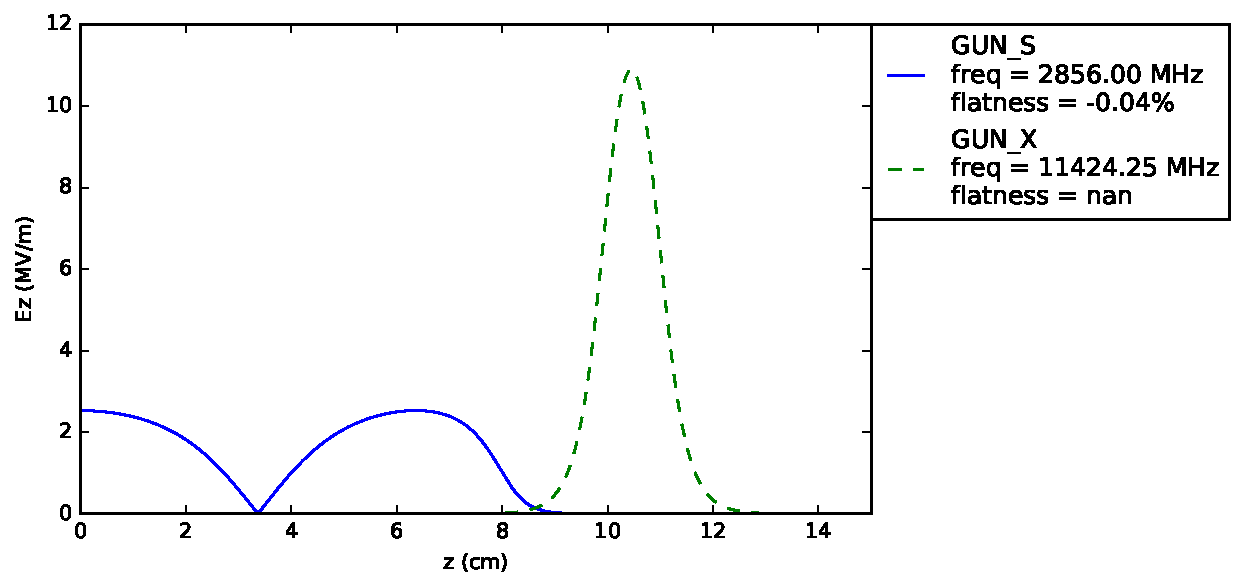
\includegraphics[width=0.8\textwidth]{sx-dist}
	\caption{
	S/X 双频电子枪中的轴线电场分布。注意纵座标并不代表实际场强,而是分别对 S 波段和 X 波段腔中模式能量进行归一化后的场强。}
	\label{fig:sx-fielddist}
\end{figure}
S/X 双频电子枪的轴线场分布见图 \ref{fig:sx-fielddist}。从图中可见,S 波段半腔和整腔中的场强基本平整,X 波段高阶模几乎没有渗透进 S 波段腔体中,自动优化算法较为可靠。另外也可看到,由于 X 波段腔的存在,S 波段整腔中场强分布变得稍稍不对称,这个不对称性对动力学的影响有待后续模拟研究。

\section{空间分离双频电子枪的动力学验证}
腔型设计好后,需要对双频电子枪的性能进行验证,我们利用 Astra 来做空间分离双频电子枪的动力学模拟。人们真正关心的是注入器出口处束流的参数而非仅仅电子枪出口处的束流参数,因此双频电子枪被放入一个类 LCLS 的光阴极注入器(见图 \ref{fig:injector-x})中进行动力学优化。为验证双频电子枪的亮度提升的效果,需要与普通电子枪的注入器优化结果进行比对。

我们关心的物理量为注入器出口处束流的峰值流强和发射度(100\% 投影发射度,95\% 投影发射度及切片发射度),在束团电荷量一定的情况下(200\,pC),注入器出口处峰值流强可以近似认为只由束团长度决定,因此最终的目标变量设置为注入器出口处束流的 rms 长度与投影发射度。如图 \ref{fig:injector-x} 中所示,整个注入器由双频电子枪,螺线管线圈及两段加速管构成,可优化的变量为:
\begin{itemize}
\item {\sf 激光}:激光长度及横向尺寸
\item {\sf 双频电子枪}:S 波段腔的场强和相位;X 波段腔的场强和相位
\item {\sf 螺线管线圈}:位置和强度
\item {\sf 加速管}:第一段加速管位置和场强;第二段加速管位置和场强
\end{itemize}
其中 S 波段腔的场强应该取可取的最大值,因为阴极表面场越强对空间电荷发射度增长的抑制效果就越好;第二段加速管一般紧贴第一段加速管,因此只要第一段加速管位置确定,第二段的位置也随之确定,不需要优化。从上面的分析看,完整的注入器需要优化 10 个变量,若采用人工方式优化不仅工作量/耗时巨大而且无法保证取到全局最优解。鉴于此,我们采用了遗传算法(Genetic Algorithm,GA)对该多变量问题进行优化。
\begin{figure}[htbp]
	\centering
	
\includegraphics[width=0.9\textwidth]{injector-x}	
	\caption{S/X 双频电子枪的注入器布局示意图。}
	\label{fig:injector-x}
\end{figure}

\subsection{遗传算法优化器}
\subsubsection{NSGA-II}
我们采用了经典而高效的算法 NSGA-II(Nondominated Sorting Genetic Algorithm II)来驱动遗传算法优化器。
\begin{figure}[htbp]
	\centering
	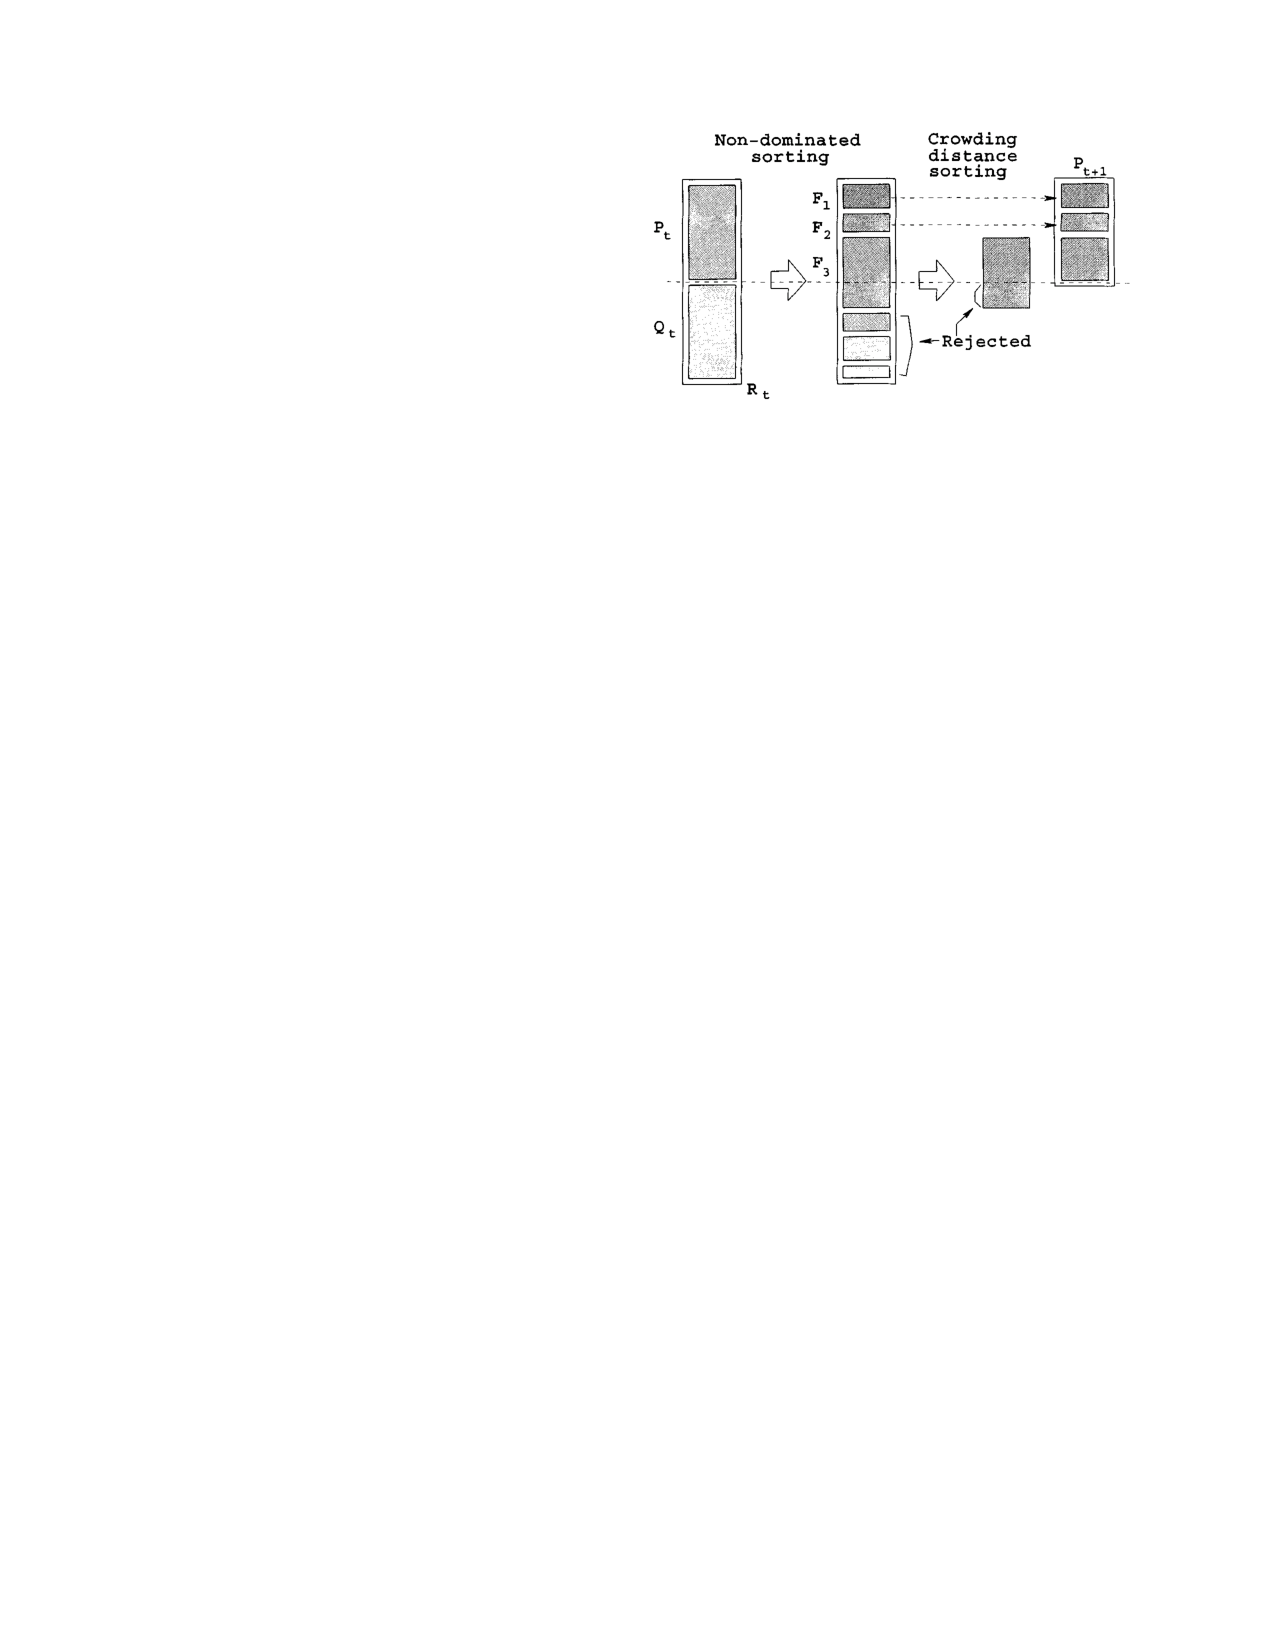
\includegraphics[width=0.6\textwidth]{nsgaii}	
	\caption{NSGA-II 算法原理示意图。}
	\label{fig:nsgaii}
\end{figure}
NSGA-II 的基本原理如图 \ref{fig:nsgaii} 所示,NSGA-II 在进化过程中,同时保留父代和子代,将相邻两代按照种群距离进行筛选,并分为一等公民,二等公民等;产生新的子代时,先从一等公民中按性状优良程度挑选,再依法炮制挑选二等公民,直至达到种群容量上限;新挑选出的子代再分成两组进行 crossover。上述过程一直进行下去,直至种群收敛,此时算法将给出一组最优解,即 Pareto 前沿。多次改变初始种群进行 NSGA-II,就可以获得全局最优解集。

\subsubsection{遗传算法优化器的逻辑结构}
遗传算法优化器逻辑上分为四部分:生成器,运行器,后处理器以及迭代器。下面首先介绍优化器的运行方式,再分别介绍四部分各自的用途。

优化器需要一个已经运行通过的模拟算例作为起始算例,该模拟算例一般体现为一个文件夹,其中包含模拟的输入文件,以及模拟所需要的场分布等附加文件。优化器运行时,对初始算例中的输入文件进行解析,给出输入文件中所有重要的可变参数,随后根据优化器配置文件中设置的具体关心的参数以及各参数的可变范围,依据初始算例,对其参数进行覆盖,随机生成给定容量的初始种群。随后优化器调用动力学模拟程序(例如 Astra)对初始种群的每个个体进行模拟,模拟结束后对模拟结果进行后处理,最后该种群的后处理结果经过汇总分析后,产生新一代种群,依此类推,直到达到优化目标或超出预设资源(时间/存储空间等),优化结束。

\red{这里要插一张流程图。}

在上面的过程中,生成器会根据迭代器提供的输入参数,基于初始算例给出新的待模拟算例;运行器负责调用动力学模拟软件对生成器给出的待模拟算例进行模拟;后处理器接受运行器模拟完成的算例,并对模拟结果进行统计,得到关心的参数(例如注入器出口处束长,发射度等);迭代器则扮演了优化过程的大脑的角色,它根据后处理器给出各算例的参数,给出下一组待模拟算例的输入参数(例如激光尺寸,腔的相位、强度等),同时迭代器还承担着控制整个优化进程的任务,也即它需要根据情况判断是否优化条件达成,是否超时/超储存空间而中止优化等。

以上是遗传算法优化器的一般逻辑结构,该结构并不仅限于遗传算法优化,而是适用于几乎一切加速器中的束流动力学模拟优化任务。在处理不同任务时,只需要根据优化目标和优化方法对迭代器进行定制即可。例如,要对束线中某个参数进行扫描,那么迭代器的逻辑就是根据待扫描参数的上一个取值,给出待扫描参数的下一个取值;对于支持并行计算的平台,实现可以更加简单和快速:迭代器初始化时直接给出待扫描参数全部可能取值,那么该扫描任务一次迭代就完成了。对于本章所采用的遗传算法而言,迭代器执行遗传算法的筛选过程,将父代中符合要求的个体留下,crossover/变异后产生下一代种群。

上面描述的优化器逻辑结构也自动具有扩展功能:例如运行器可以支持调用各种模拟软件,如 Astra,GPT,Parmela 等,只需要为相应的模拟软件写好调用接口即可;而迭代器的具体实现也可以多种多样,甚至可以由人来担任迭代器,根据后处理器给出的上一代性能,决定下一代的优化方向。

\subsubsection{遗传算法优化器的编程实现}
我们采用 Python 编程实现了遗传算法优化器的逻辑结构。优化器程序分为以下六个文件:
\begin{itemize}
\item {\sf astracore.py}:生成器与运行器,负责读取初始模拟算例,接受输入参数生成新算例以及调用 Astra 程序进行模拟计算
\item {\sf plotplugins.py}:后处理器的图形部分,负责对模拟结果进行可视化,例如画出横/纵向相空间,束团纵向密度分布等
\item {\sf statplugins.py}:后处理器的统计部分,负责对模拟结果进行统计,给出发射度/能散/束长/切片发射度等参数
\item {\sf physicshelper.py}:基础的物理运算助手,进行如波长/能量转换,时间/长度转换及 $\beta$/$\gamma$ 等相对论因子转换等常见运算
\item {\sf gaoptimizer.py}:迭代器的引擎,实现了 NSGA-II 算法
\item {\sf main.py}:优化器入口,迭代器的流程控制逻辑,负责产生初始种群,利用 NSGA-II 引擎进化种群,并在满足一定条件后中止进化并产生断点;支持从断点处继续进化的功能
\end{itemize}
遗传算法优化器的核心文件是 {\sf gaoptimizer.py},其内部采用了 DEAP 库作为遗传算法支持库,采用 SCOOP 库实现多核并行计算。有了并行计算的支持,遗传算法优化器才有应用的可能。{\sf main.py} 是遗传算法优化器的入口,其中配置了束线信息,输入变量,优化目标以及遗传算法参数等信息,要应用遗传算法优化器进行束线优化,只需要修改 {\sf main.py} 文件即可。

\subsubsection{遗传算法优化器的运行流程}
遗传算法优化器需要运行在支持并行运算的大型机上。假设占用大型机的 N 个处理器核,其中一个核为主核,其它核为附属核(worker)。一次优化开始时,优化器向主核提交任务,主核调用迭代器产生容量为 N 的初始种群,并调用生成器产生全部模拟算例;随后将每个算例分配到不同的核上,调用运行器进行模拟;所有核上的模拟并行进行,各核之间在模拟过程中无数据交换。注入器在不同输入参数下模拟时间会有伸缩(例如某些电子枪相位可能导致束团反轰,模拟会提前结束),而下一代种群的基因产生需要等上一代模拟彻底结束后才能开始,因此种群的模拟时间等于该种群中耗时最长的个体所用的模拟时间。当种群中全部个体均模拟完毕,各核将模拟结果返回给主核,主核调用后处理器对模拟结果进行后处理(一般是统计注入器出口处 rms 束流长度核 100\% 投影发射度),并将各算例的数据处理结果汇总,调用迭代器根据 NSGA-II 的规则进行筛选、crossover 以及变异,产生下一代种群。循环上面步骤,直到满足跳出条件或达到优化目标,就完成一次遗传算法优化。

遗传算法优化器在每一代种群模拟结束后,都会将该代种群的后处理结果写入一个名为 {\sf ghist} 的文件中,因此即使优化突然中断,{\sf ghist} 文件也保存了从初代种群到中断前种群的全部历史;再次启动优化时,优化器会首先尝试读取 {\sf ghist} 文件,并以最近的一代种群作为起点,继续进化。这就是从断点继续进化的实现原理。

\subsection{遗传算法优化平台}
为保证优化时间在可接受的范围内,我们采用了清华大学探索 100 高性能计算平台作为遗传算法优化器的运行平台。探索 100 高性能平台共有 740 个计算节点,8800 个处理器核。处理器核按照刀片(board)组织,一个刀片上有 12 颗处理器核,一个刀片对应一个计算节点;刀片按照刀片箱(cabinet)放置,每个刀片箱有 20 个刀片,共有 37 个刀片箱。因此定位某计算节点时,采用 c[xx]b[yy] 的方式,其中 [xx] 和 [yy] 为数字,例如 c01b02 就是第一个刀片箱的第二块刀片对应的计算节点。

对于遗传算法驱动的双频电子枪注入器动力学优化,一般选取种群容量是 12 的整数倍(这样就可以占用若干完整的刀片进行并行计算,由于同一个刀片上各核间的数据传输速度远高于不同刀片核间的数据传输速度,占用完整的刀片可使模拟数据的传输更快),为保证 Pareto 前沿的覆盖性,种群容量不能太小,因此常用 120、240 以及 360 的种群容量;探索 100 的处理器是 Intel Xeon X5670,主频 2.93\,GHz,缓存 12\,MB,此配置下采用较多的宏粒子数(20000--30000)对图 \ref{fig:injector-x} 中所示注入器的单次模拟时间大约在 30 分钟到 60 分钟之间;遗传算法收敛所需代数依据遗传算法参数(如 crossover 概率,突变概率等等)不同而不同,但一般 100 到 200 代就可以收敛,获得较稳定的 Pareto 前沿。综上所述,完成一次完整的注入器遗传算法优化只需要 2 天到 8 天,对于多输入变量多优化目标问题而言,相对于人工优化不仅时间更短,而且可以一次得到一批优化解,在优化效率上有巨大优势。

\subsection{基于遗传算法的双频电子枪注入器动力学优化}

\begin{figure}[htbp]
	\centering
	
\includegraphics[width=0.9\textwidth]{injector-c}	
	\caption{分离型 S/C 双频电子枪的注入器布局示意图。}
	\label{fig:injector-c}
\end{figure}

\subsubsection{S/C 分离型双频枪注入器}
基于上面的理由,我们考虑了分离型的双频电子枪,即螺线管线圈置于 S 波段电子枪与 C 波段聚束腔之间。我们采用了遗传算法优化器对 \SI{200}{pC} 束团电荷量的情形进行了优化。

光阴极注入器束线设置见图 \ref{fig:injector-c},其包括一个 BNL 型 S 波段电子枪(腔梯度设置为 \SI{120}{MV/m}),一个发射度补偿螺线管线圈,一个 C 波段聚束腔和两节 S 波段行波加速管(每节加速管加速梯度 $<$ \SI{78}{MV})。光阴极上的激光纵向分布为平顶分布,其上升和下降时间均设置为束团半高全宽的 10\%,横向分布为在一倍标准差处截断的高斯分布。激光的横向/纵向尺寸,枪相位,螺线管线圈强度,C 波段聚束腔位置、梯度及相位,行波加速管的梯度和位置作为优化器的待优化变量。

注入器出口处 100\% 发射度和 rms 束团长度作为优化的目标变量,且其优化方向为趋向最小值。我们也对束流能量做了限制(注入器出口处束流能量不低于 \SI{100}{MeV})。优化结果的 Pareto 前沿如图 \ref{Pareto120}(a)所示,图中 \SI{0.65}{mm} 的 rms 束团长度就对应 \SI{30}{A} 的峰值电流。图 \ref{Pareto120} 清晰地显示,通过引入一个 C 波段聚束腔,注入器出口处的发射度得以在 \SI{30}{A} 峰值流强下较无聚束腔情形降低了 $\sim$25\%。图 \ref{Pareto120}(b)中我们画出了优化解集对应的 95\% 投影发射度(近似等于去掉头尾切片后束流的 100\% 投影发射度)与 rms 束长的拮抗关系,图中的绿色三角形代表了相应的优化解对应的初始热发射度,可以看出,加入了 C 波段聚束腔的注入器束线出口处的 95\% 发射度与阴极产生的初始热发射度相当接近,这说明阴极表面的束团亮度被保持到了注入器出口。

\begin{figure}[htbp]
	\centering
	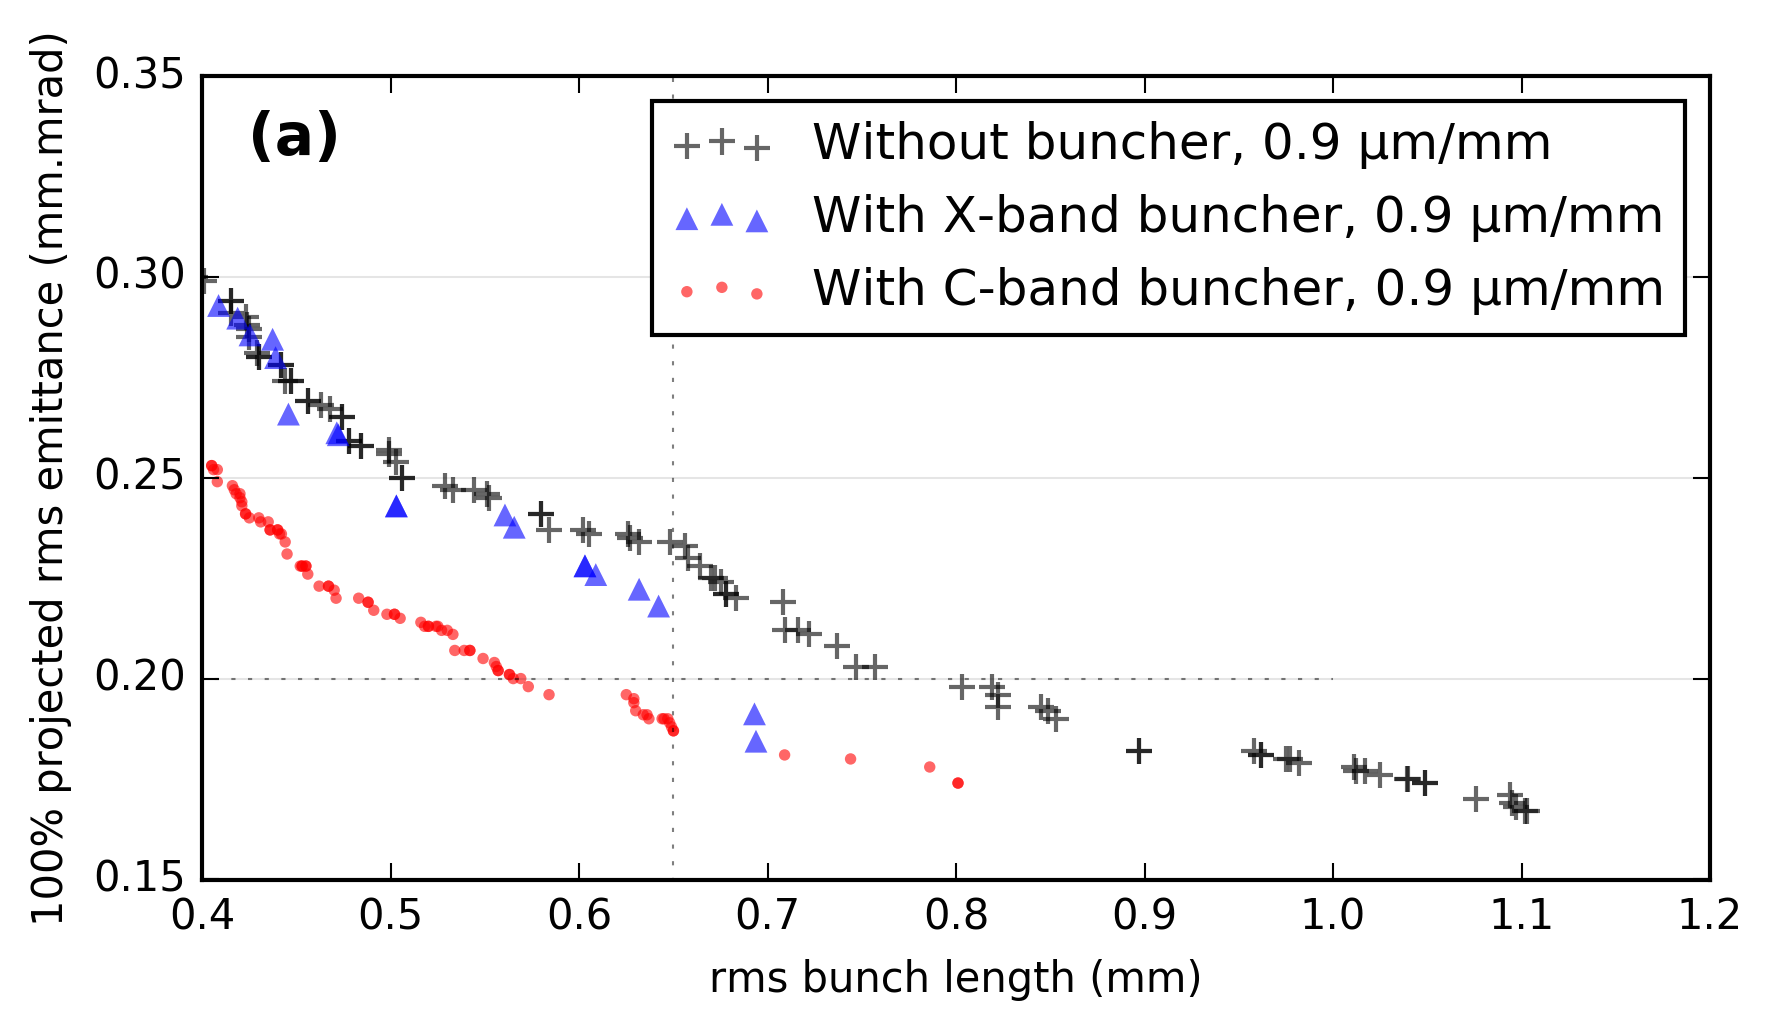
\includegraphics[width=0.6\textwidth]{s120-a}\\
	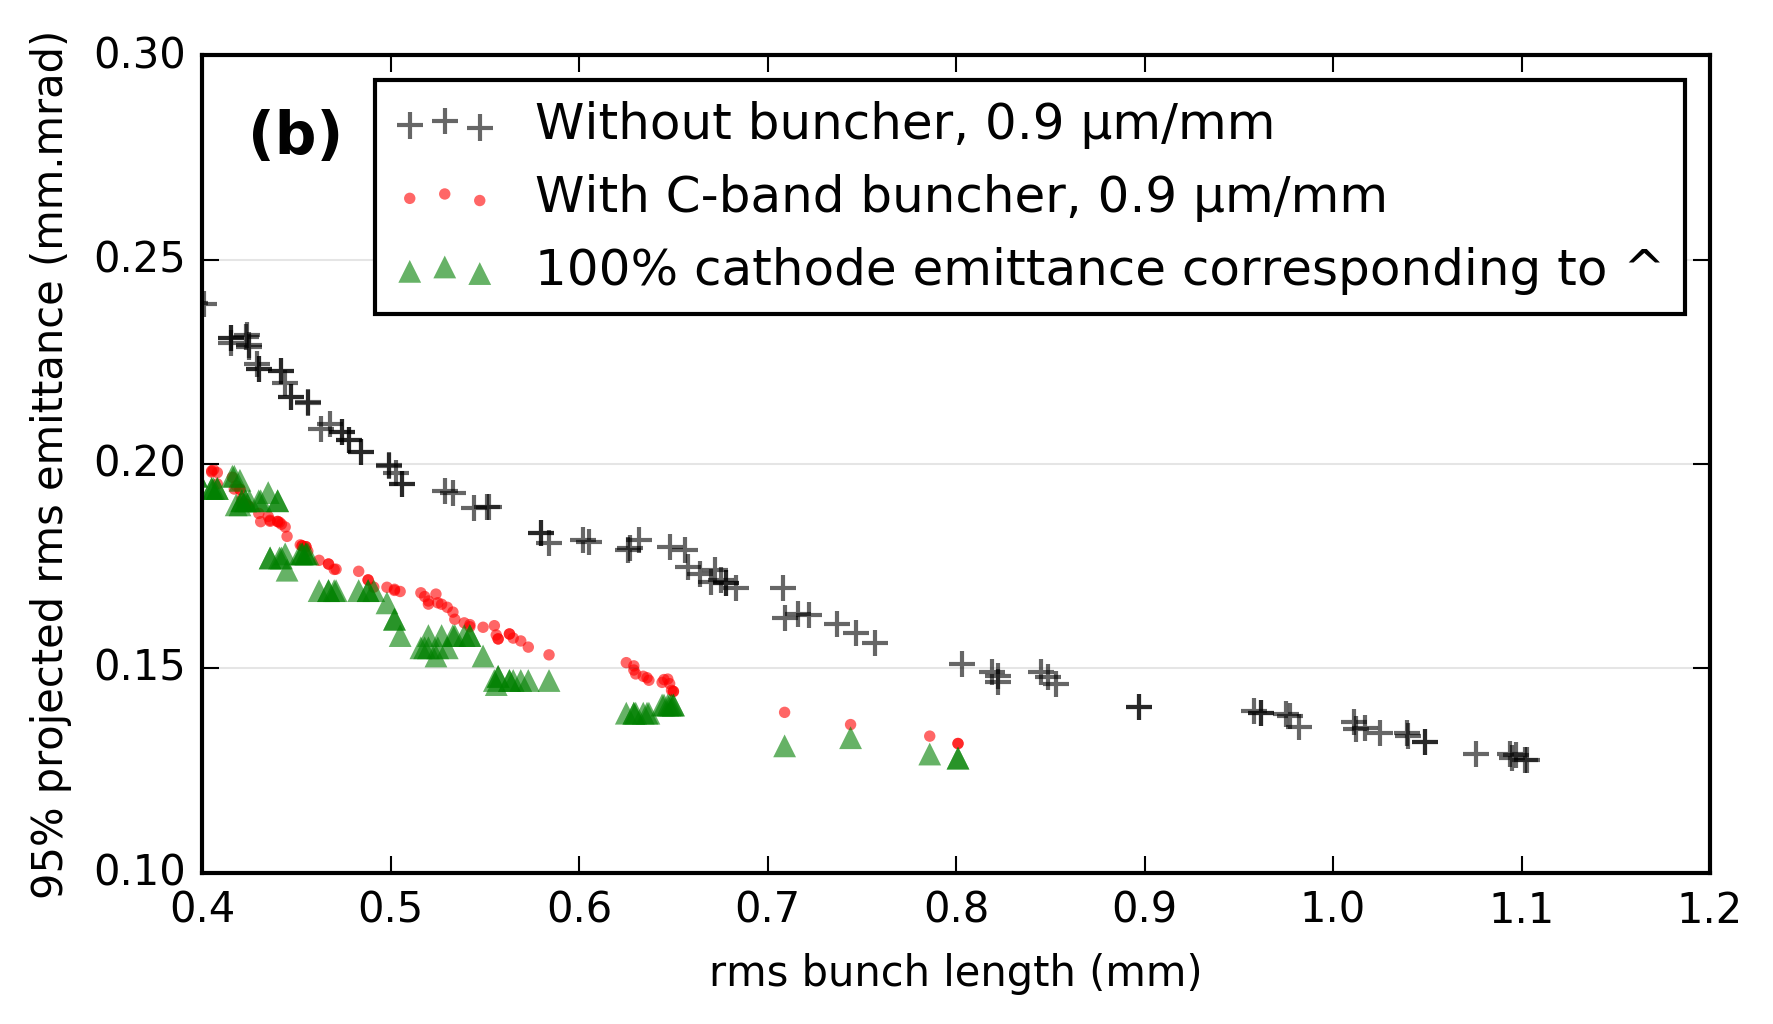
\includegraphics[width=0.6\textwidth]{s120-b}
	\caption{
	200\,pC 束团发射度 vs. rms 长度的一组最优解集。Astra 模拟中采用 10000 宏粒子。图中同时比较了 S 波段光阴极注入器加入 C 波段高频腔与否的发射度优化情形。}
	\label{Pareto120}
\end{figure}

图 \ref{laser_dimension} 是图 \ref{Pareto120} 中给出的优化解集所对应的激光尺寸参数。从图中可以看到,集成了高频腔后,电子枪拥有了在枪的下游对束团进行压缩的能力,从而保持相同的注入器出口峰值流强时,阴极表面的束流峰值流强就可以降低,因此激光纵向可以拉长,由于电荷密度基本不变,其横向尺寸可以缩小,这就减小了阴极上的热发射度。图上对应 \SI{30}{A} 峰值流强的位置,相较于无高频腔的情形其对应激光长度从 \SI{5}{ps} 拉长到了 \SI{10}{ps},而激光半径 $r$ 从 \SI{0.4}{mm} 降低到了 \SI{0.32}{mm}。若此时发射为笔形束的饱和发射情形,则激光长度与 $r^{3/2}$ 成反比,因此当激光长度拉长一倍时,激光半径的减小比例应为 37\%,然而如前所述,遗传算法优化器选择了 20\% 的减小量,这就暗示了引入了聚束腔后,笔形束的饱和发射(此时阴极束流亮度最高)并不是使注入器出口处亮度最高的情形;而对于无聚束腔的注入器优化结果证明阴极束流亮度最高的同时注入器出口处也取到最高亮度。引入聚束腔而导致的阴极束流最高亮度无法保持的现象的原因需要进一步探索。

图 \ref{laser_dimension} 还表明另一个现象:即使引入聚束腔,激光的束长也没有达到优化中设置的上限值 15\,ps。目前怀疑这是由于初始束团过长导致较大 RF 能散在螺线管线圈中的色散效应造成的。具体原因也有待进一步研究。

图 \ref{Pareto120} 中对应 \SI{30}{A} 峰值流强的优化解的切片发射度见图 \ref{slice_emittance}。图中可以看到,在加入一个聚束腔后,除头尾外整个束团的切片发射度较为统一,均在 \SI{0.15}{\mu m} 附近;相对于无聚束腔的情形,切片发射度得到了 25\% 的减小,且各切片的发射度也更加均匀。若设法将热发射度从 \SI{0.9}{\mu m/mm} 降至 \SI{0.5}{\mu m/mm},优化器给出的核心切片发射度可以降至 \SI{0.1}{\mu m}。图中显示无聚束腔情形核心切片发射度均在 \SI{0.2}{\mu m} 以上,这也说明了当前注入器出口处束流发射度最低也只能测到 \SI{0.2}{\mu m} 左右的原因。

\begin{figure}[htbp]
	\centering
	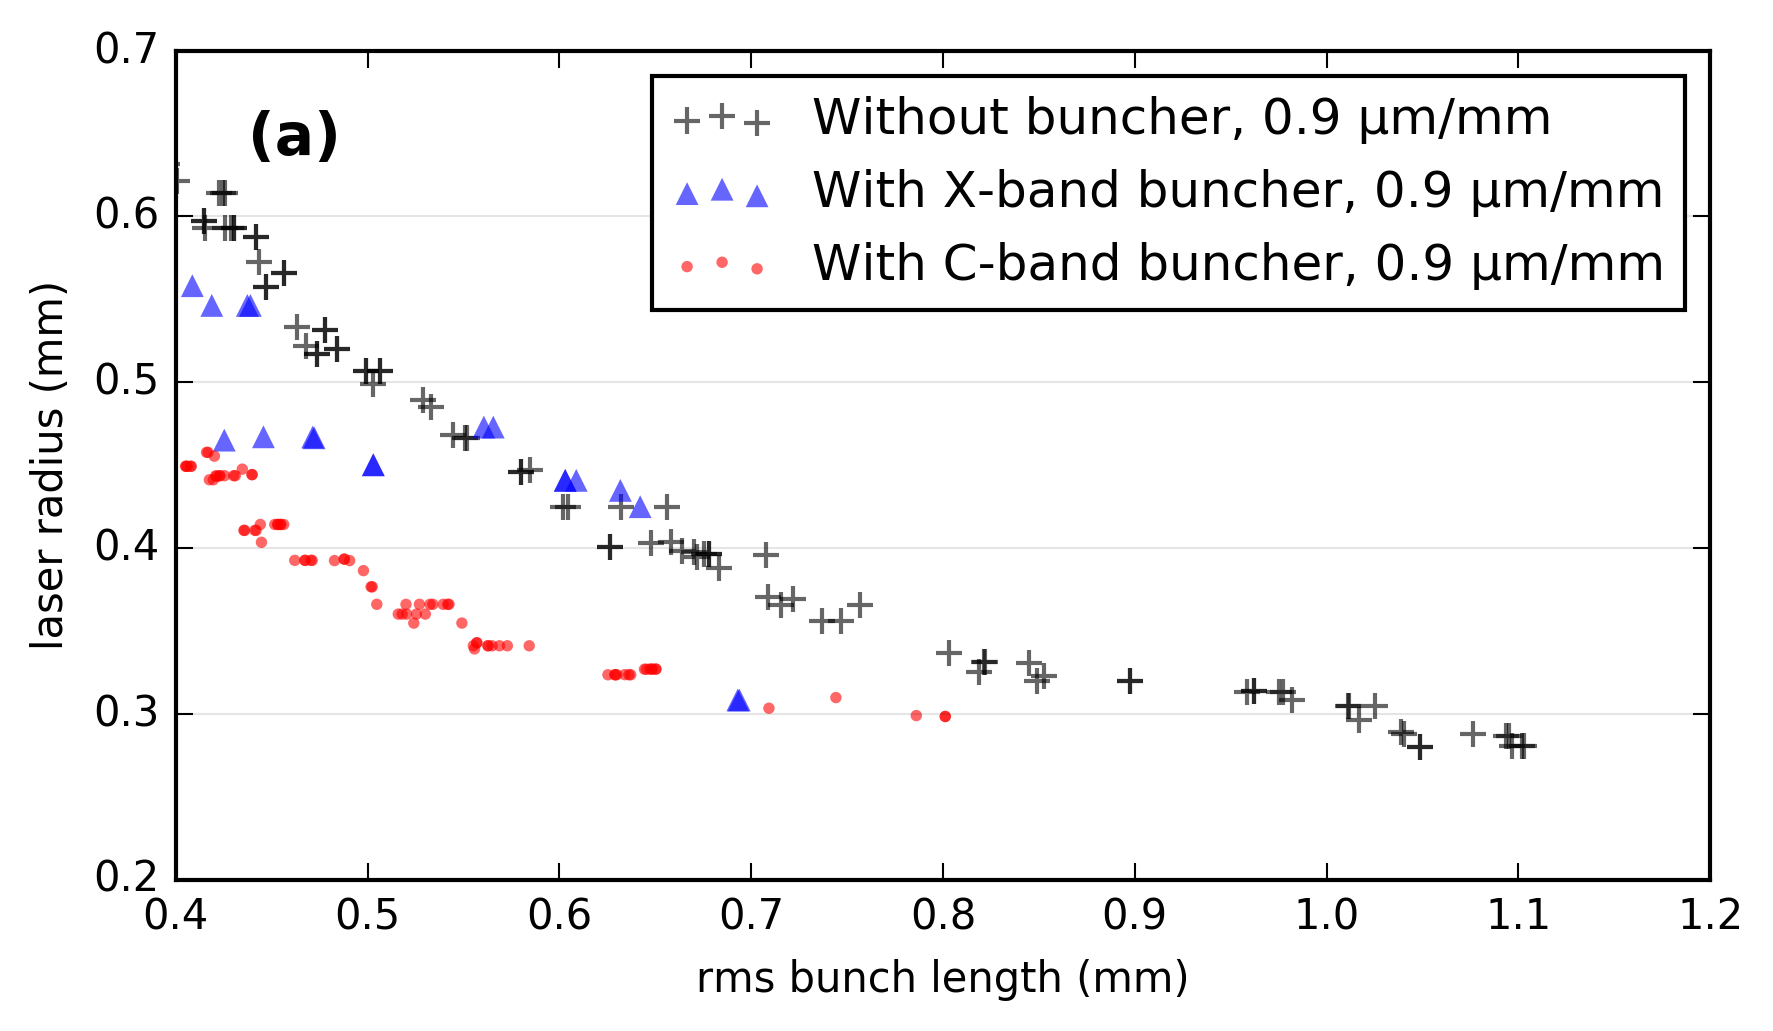
\includegraphics[width=0.6\textwidth]{laser-a}\\
	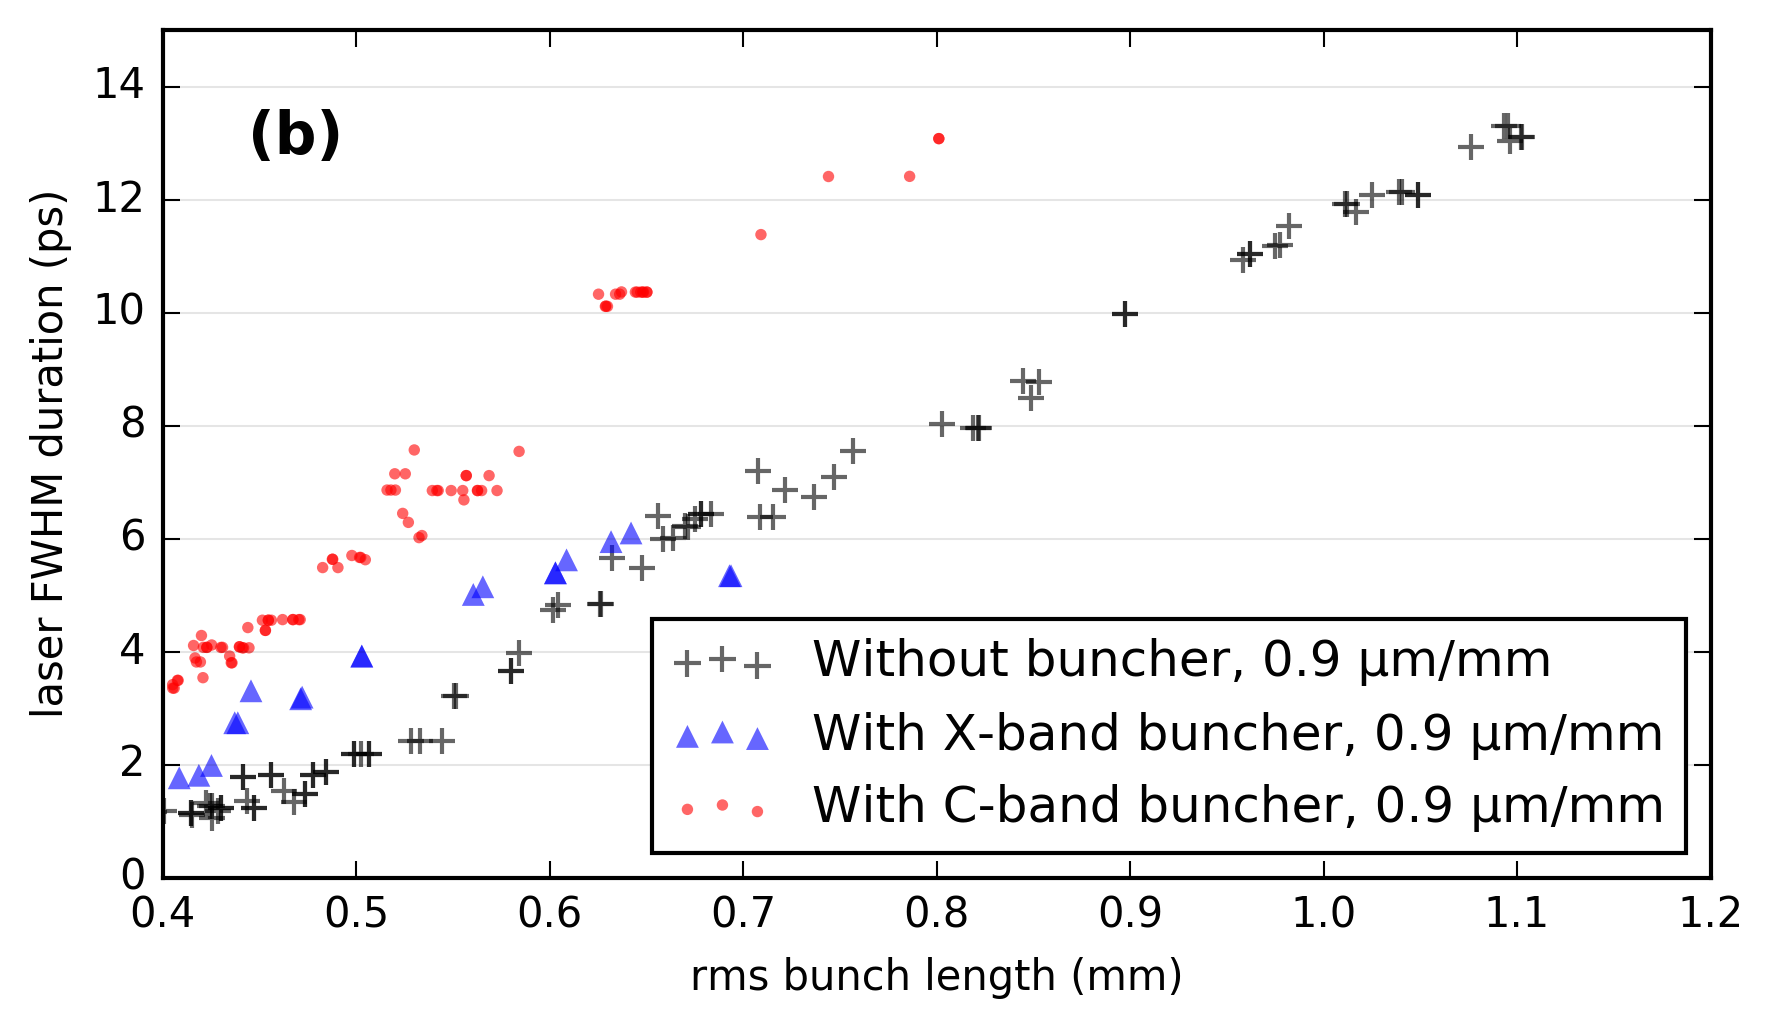
\includegraphics[width=0.6\textwidth]{laser-b}
	\caption{图 \ref{Pareto120} 给出优化结果所对应的激光半径和 FWHM 长度。}
	\label{laser_dimension}
\end{figure}

\begin{figure}[htbp]
	\centering
	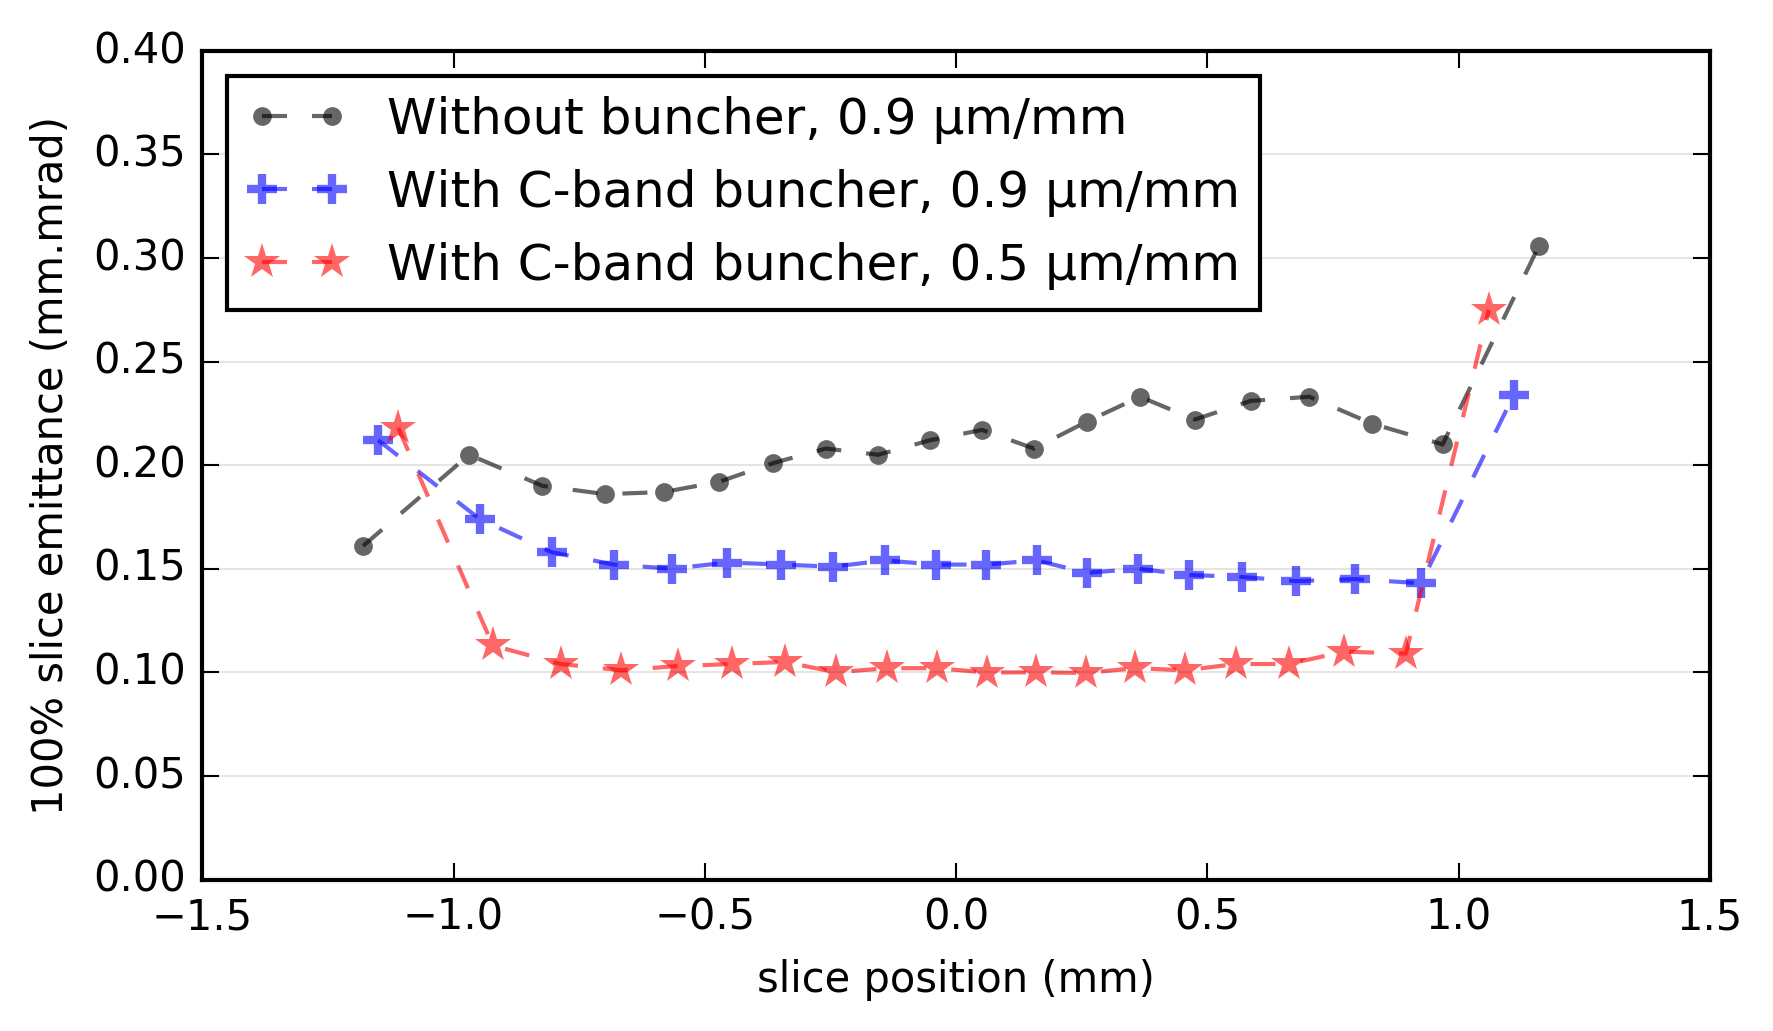
\includegraphics[width=0.6\textwidth]{slice}
	\caption{\SI{200}{pC} 束团,注入器出口处 \SI{30}{A} 峰值流强的优化解的切片发射度。Astra 模拟中采用了 20000 宏粒子。}
	\label{slice_emittance}
\end{figure}

\subsubsection{S/X 合并型双频腔注入器}
我们首先用遗传算法优化器优化了合并型 S/X 双频电子枪注入器,其束线布局见图 \ref{fig:injector-x}。束线包括一个 BNL 型 S 波段电子枪(腔梯度设置为 \SI{120}{MV/m}),一个发射度补偿螺线管线圈,一个 X 波段聚束腔和两节 S 波段行波加速管(每节加速管加速梯度 $<$ \SI{78}{MV})。光阴极上的激光纵向分布为均匀分布,横向分布为在一倍标准差处截断的高斯分布。激光的横向/纵向尺寸,S 波段电子枪相位,X 波段聚束腔梯度及相位,螺线管线圈强度,行波加速管的梯度和位置作为优化器的待优化变量。

图 \ref{Pareto120}(a)比较了 S/X 双频腔注入器、S/C 双频腔注入器与 S 波段电子枪注入器的 Pareto 前沿。从图中可以看到,在 rms 束团长度小于 \SI{0.65}{mm}(峰值流强小于 \SI{30}{A})时,加入 X 波段聚束腔的优化结果趋近于无聚束腔的情形,当 rms 束团长度大于 \SI{0.65}{mm},X 波段聚束腔的优化结果趋向于 C 波段聚束腔的优化结果。分离型和合并型双频电子枪性能的差异有待进一步分析。

\subsubsection{高频腔选取不同波段的优化结果对比}

\subsubsection{分离型和合并型双频电子枪性能差异的分析}

\section{非线性发射区注入器束流亮度的研究}

\section{小结}
By adding a harmonic buncher either before or after the emittance compensation solenoid, a two frequency photoinjector is proposed to further improve beam brightness by using cigar beam photoemission. Both the initial RF design and beam dynamics investigations with a GA optimizer are presented. The preliminary simulation results show that with a HOM cavity added, the emittance at injector exit can be reduced by $\sim$25\% at \SI{30}{A} peak current for \SI{200}{pC}, and slice emittance can be reduced to $\sim$\emit{0.10} with a  \SI{0.5}{\mu m/mm} thermal emittance. Nevertheless there're several issues yet to be solved. To name a few, the GA optimizer chooses not to take full advantage of the buncher by lengthening the laser pulse beyond \SI{10}{ps}; putting the buncher downstream the solenoid could achieve smaller emittance compared with buncher before the solenoid. We would continue to investigate the mechanisms behind all these issues in order to further improve the beam emittance.

%!TEX root = ../main.tex
\chapter{总结与展望}
\label{chap:summary}



%%% 其它部分
\backmatter

%% 本科生要这几个索引,研究生不要。选择性留下。
% 插图索引
% \listoffigures
% 表格索引
% \listoftables
% 公式索引
% \listofequations


%% 参考文献
% 注意:至少需要引用一篇参考文献,否则下面两行可能引起编译错误。
% 如果不需要参考文献,请将下面两行删除或注释掉。
% \bibliographystyle{thuthesis}
% \bibliography{ref/refs}


%% 致谢
%!TEX root = ../main.tex
% 如果使用声明扫描页,将可选参数指定为扫描后的 PDF 文件名,例如:
% \begin{ack}[scan-statement.pdf]
\begin{acknowledgement}
  衷心感谢导师唐传祥教授对本人的精心指导。他的言传身教将使我终生受益。

  在美国 UCLA 物理与天文学系 Pegasus 实验室进行九个月的合作研究期间,承蒙 Musumeci Pietro 副教授热心指导与帮助,不胜感激。感谢加速器实验室主任黄文会教授,以及实验室全体老师和同学们的热情帮助和支持!本课题承蒙国家自然科学基金资助,特此致谢。

  感谢 \thuthesis,它的存在让我的论文写作轻松自在了许多,让我的论文格式规整漂亮了许多。
\end{acknowledgement}


%% 附录
\begin{appendix}
\chapter{外文资料原文}
\label{cha:engorg}

\title{The title of the English paper}

\textbf{Abstract:} As one of the most widely used techniques in operations
research, \emph{ mathematical programming} is defined as a means of maximizing a
quantity known as \emph{bjective function}, subject to a set of constraints
represented by equations and inequalities. Some known subtopics of mathematical
programming are linear programming, nonlinear programming, multiobjective
programming, goal programming, dynamic programming, and multilevel
programming$^{[1]}$.

It is impossible to cover in a single chapter every concept of mathematical
programming. This chapter introduces only the basic concepts and techniques of
mathematical programming such that readers gain an understanding of them
throughout the book$^{[2,3]}$.


\section{Single-Objective Programming}
The general form of single-objective programming (SOP) is written
as follows,
\begin{equation}\tag*{(123)} % 如果附录中的公式不想让它出现在公式索引中,那就请
                             % 用 \tag*{xxxx}
\left\{\begin{array}{l}
\max \,\,f(x)\\[0.1 cm]
\mbox{subject to:} \\ [0.1 cm]
\qquad g_j(x)\le 0,\quad j=1,2,\cdots,p
\end{array}\right.
\end{equation}
which maximizes a real-valued function $f$ of
$x=(x_1,x_2,\cdots,x_n)$ subject to a set of constraints.

\newtheorem{mpdef}{Definition}[chapter]
\begin{mpdef}
In SOP, we call $x$ a decision vector, and
$x_1,x_2,\cdots,x_n$ decision variables. The function
$f$ is called the objective function. The set
\begin{equation}\tag*{(456)} % 这里同理,其它不再一一指定。
S=\left\{x\in\Re^n\bigm|g_j(x)\le 0,\,j=1,2,\cdots,p\right\}
\end{equation}
is called the feasible set. An element $x$ in $S$ is called a
feasible solution.
\end{mpdef}

\newtheorem{mpdefop}[mpdef]{Definition}
\begin{mpdefop}
A feasible solution $x^*$ is called the optimal
solution of SOP if and only if
\begin{equation}
f(x^*)\ge f(x)
\end{equation}
for any feasible solution $x$.
\end{mpdefop}

One of the outstanding contributions to mathematical programming was known as
the Kuhn-Tucker conditions\ref{eq:ktc}. In order to introduce them, let us give
some definitions. An inequality constraint $g_j(x)\le 0$ is said to be active at
a point $x^*$ if $g_j(x^*)=0$. A point $x^*$ satisfying $g_j(x^*)\le 0$ is said
to be regular if the gradient vectors $\nabla g_j(x)$ of all active constraints
are linearly independent.

Let $x^*$ be a regular point of the constraints of SOP and assume that all the
functions $f(x)$ and $g_j(x),j=1,2,\cdots,p$ are differentiable. If $x^*$ is a
local optimal solution, then there exist Lagrange multipliers
$\lambda_j,j=1,2,\cdots,p$ such that the following Kuhn-Tucker conditions hold,
\begin{equation}
\label{eq:ktc}
\left\{\begin{array}{l}
    \nabla f(x^*)-\sum\limits_{j=1}^p\lambda_j\nabla g_j(x^*)=0\\[0.3cm]
    \lambda_jg_j(x^*)=0,\quad j=1,2,\cdots,p\\[0.2cm]
    \lambda_j\ge 0,\quad j=1,2,\cdots,p.
\end{array}\right.
\end{equation}
If all the functions $f(x)$ and $g_j(x),j=1,2,\cdots,p$ are convex and
differentiable, and the point $x^*$ satisfies the Kuhn-Tucker conditions
(\ref{eq:ktc}), then it has been proved that the point $x^*$ is a global optimal
solution of SOP.

\subsection{Linear Programming}
\label{sec:lp}

If the functions $f(x),g_j(x),j=1,2,\cdots,p$ are all linear, then SOP is called
a {\em linear programming}.

The feasible set of linear is always convex. A point $x$ is called an extreme
point of convex set $S$ if $x\in S$ and $x$ cannot be expressed as a convex
combination of two points in $S$. It has been shown that the optimal solution to
linear programming corresponds to an extreme point of its feasible set provided
that the feasible set $S$ is bounded. This fact is the basis of the {\em simplex
  algorithm} which was developed by Dantzig as a very efficient method for
solving linear programming.
\begin{table}[ht]
\centering
  \centering
  \caption*{Table~1\hskip1em This is an example for manually numbered table, which
    would not appear in the list of tables}
  \label{tab:badtabular2}
  \begin{tabular}[c]{|m{1.5cm}|c|c|c|c|c|c|}\hline
    \multicolumn{2}{|c|}{Network Topology} & \# of nodes &
    \multicolumn{3}{c|}{\# of clients} & Server \\\hline
    GT-ITM & Waxman Transit-Stub & 600 &
    \multirow{2}{2em}{2\%}&
    \multirow{2}{2em}{10\%}&
    \multirow{2}{2em}{50\%}&
    \multirow{2}{1.2in}{Max. Connectivity}\\\cline{1-3}
    \multicolumn{2}{|c|}{Inet-2.1} & 6000 & & & &\\\hline
    \multirow{2}{1.5cm}{Xue} & Rui  & Ni &\multicolumn{4}{c|}{\multirow{2}*{\thuthesis}}\\\cline{2-3}
    & \multicolumn{2}{c|}{ABCDEF} &\multicolumn{4}{c|}{} \\\hline
\end{tabular}
\end{table}

Roughly speaking, the simplex algorithm examines only the extreme points of the
feasible set, rather than all feasible points. At first, the simplex algorithm
selects an extreme point as the initial point. The successive extreme point is
selected so as to improve the objective function value. The procedure is
repeated until no improvement in objective function value can be made. The last
extreme point is the optimal solution.

\subsection{Nonlinear Programming}

If at least one of the functions $f(x),g_j(x),j=1,2,\cdots,p$ is nonlinear, then
SOP is called a {\em nonlinear programming}.

A large number of classical optimization methods have been developed to treat
special-structural nonlinear programming based on the mathematical theory
concerned with analyzing the structure of problems.
\begin{figure}[h]
  \centering
  
\includegraphics{thu-lib-logo}
  \caption*{Figure~1\quad This is an example for manually numbered figure,
    which would not appear in the list of figures}
  \label{tab:badfigure2}
\end{figure}

Now we consider a nonlinear programming which is confronted solely with
maximizing a real-valued function with domain $\Re^n$.  Whether derivatives are
available or not, the usual strategy is first to select a point in $\Re^n$ which
is thought to be the most likely place where the maximum exists. If there is no
information available on which to base such a selection, a point is chosen at
random. From this first point an attempt is made to construct a sequence of
points, each of which yields an improved objective function value over its
predecessor. The next point to be added to the sequence is chosen by analyzing
the behavior of the function at the previous points. This construction continues
until some termination criterion is met. Methods based upon this strategy are
called {\em ascent methods}, which can be classified as {\em direct methods},
{\em gradient methods}, and {\em Hessian methods} according to the information
about the behavior of objective function $f$. Direct methods require only that
the function can be evaluated at each point. Gradient methods require the
evaluation of first derivatives of $f$. Hessian methods require the evaluation
of second derivatives. In fact, there is no superior method for all
problems. The efficiency of a method is very much dependent upon the objective
function.

\subsection{Integer Programming}

{\em Integer programming} is a special mathematical programming in which all of
the variables are assumed to be only integer values. When there are not only
integer variables but also conventional continuous variables, we call it {\em
  mixed integer programming}. If all the variables are assumed either 0 or 1,
then the problem is termed a {\em zero-one programming}. Although integer
programming can be solved by an {\em exhaustive enumeration} theoretically, it
is impractical to solve realistically sized integer programming problems. The
most successful algorithm so far found to solve integer programming is called
the {\em branch-and-bound enumeration} developed by Balas (1965) and Dakin
(1965). The other technique to integer programming is the {\em cutting plane
  method} developed by Gomory (1959).

\hfill\textit{Uncertain Programming\/}\quad(\textsl{BaoDing Liu, 2006.2})

\section*{References}
\noindent{\itshape NOTE: These references are only for demonstration. They are
  not real citations in the original text.}

\begin{translationbib}
\item Donald E. Knuth. The \TeX book. Addison-Wesley, 1984. ISBN: 0-201-13448-9
\item Paul W. Abrahams, Karl Berry and Kathryn A. Hargreaves. \TeX\ for the
  Impatient. Addison-Wesley, 1990. ISBN: 0-201-51375-7
\item David Salomon. The advanced \TeX book.  New York : Springer, 1995. ISBN:0-387-94556-3
\end{translationbib}

\chapter{外文资料的调研阅读报告或书面翻译}

\title{英文资料的中文标题}

{\heiti 摘要:} 本章为外文资料翻译内容。如果有摘要可以直接写上来,这部分好像没有
明确的规定。

\section{单目标规划}
北冥有鱼,其名为鲲。鲲之大,不知其几千里也。化而为鸟,其名为鹏。鹏之背,不知其几
千里也。怒而飞,其翼若垂天之云。是鸟也,海运则将徙于南冥。南冥者,天池也。
\begin{equation}\tag*{(123)}
 p(y|\mathbf{x}) = \frac{p(\mathbf{x},y)}{p(\mathbf{x})}=
\frac{p(\mathbf{x}|y)p(y)}{p(\mathbf{x})}
\end{equation}

吾生也有涯,而知也无涯。以有涯随无涯,殆已!已而为知者,殆而已矣!为善无近名,为
恶无近刑,缘督以为经,可以保身,可以全生,可以养亲,可以尽年。

\subsection{线性规划}
庖丁为文惠君解牛,手之所触,肩之所倚,足之所履,膝之所倚,砉然响然,奏刀騞然,莫
不中音,合于桑林之舞,乃中经首之会。
\begin{table}[ht]
\centering
  \centering
  \caption*{表~1\hskip1em 这是手动编号但不出现在索引中的一个表格例子}
  \label{tab:badtabular3}
  \begin{tabular}[c]{|m{1.5cm}|c|c|c|c|c|c|}\hline
    \multicolumn{2}{|c|}{Network Topology} & \# of nodes &
    \multicolumn{3}{c|}{\# of clients} & Server \\\hline
    GT-ITM & Waxman Transit-Stub & 600 &
    \multirow{2}{2em}{2\%}&
    \multirow{2}{2em}{10\%}&
    \multirow{2}{2em}{50\%}&
    \multirow{2}{1.2in}{Max. Connectivity}\\\cline{1-3}
    \multicolumn{2}{|c|}{Inet-2.1} & 6000 & & & &\\\hline
    \multirow{2}{1.5cm}{Xue} & Rui  & Ni &\multicolumn{4}{c|}{\multirow{2}*{\thuthesis}}\\\cline{2-3}
    & \multicolumn{2}{c|}{ABCDEF} &\multicolumn{4}{c|}{} \\\hline
\end{tabular}
\end{table}

文惠君曰:“嘻,善哉!技盖至此乎?”庖丁释刀对曰:“臣之所好者道也,进乎技矣。始臣之
解牛之时,所见无非全牛者;三年之后,未尝见全牛也;方今之时,臣以神遇而不以目视,
官知止而神欲行。依乎天理,批大郤,导大窾,因其固然。技经肯綮之未尝,而况大坬乎!
良庖岁更刀,割也;族庖月更刀,折也;今臣之刀十九年矣,所解数千牛矣,而刀刃若新发
于硎。彼节者有间而刀刃者无厚,以无厚入有间,恢恢乎其于游刃必有余地矣。是以十九年
而刀刃若新发于硎。虽然,每至于族,吾见其难为,怵然为戒,视为止,行为迟,动刀甚微,
謋然已解,如土委地。提刀而立,为之而四顾,为之踌躇满志,善刀而藏之。”

文惠君曰:“善哉!吾闻庖丁之言,得养生焉。”


\subsection{非线性规划}
孔子与柳下季为友,柳下季之弟名曰盗跖。盗跖从卒九千人,横行天下,侵暴诸侯。穴室枢
户,驱人牛马,取人妇女。贪得忘亲,不顾父母兄弟,不祭先祖。所过之邑,大国守城,小
国入保,万民苦之。孔子谓柳下季曰:“夫为人父者,必能诏其子;为人兄者,必能教其弟。
若父不能诏其子,兄不能教其弟,则无贵父子兄弟之亲矣。今先生,世之才士也,弟为盗
跖,为天下害,而弗能教也,丘窃为先生羞之。丘请为先生往说之。”
\begin{figure}[h]
  \centering
  
\includegraphics{thu-whole-logo}
  \caption*{图~1\hskip1em 这是手动编号但不出现索引中的图片的例子}
  \label{tab:badfigure3}
\end{figure}

柳下季曰:“先生言为人父者必能诏其子,为人兄者必能教其弟,若子不听父之诏,弟不受
兄之教,虽今先生之辩,将奈之何哉?且跖之为人也,心如涌泉,意如飘风,强足以距敌,
辩足以饰非。顺其心则喜,逆其心则怒,易辱人以言。先生必无往。”

孔子不听,颜回为驭,子贡为右,往见盗跖。

\subsection{整数规划}
盗跖乃方休卒徒大山之阳,脍人肝而餔之。孔子下车而前,见谒者曰:“鲁人孔丘,闻将军
高义,敬再拜谒者。”谒者入通。盗跖闻之大怒,目如明星,发上指冠,曰:“此夫鲁国之
巧伪人孔丘非邪?为我告之:尔作言造语,妄称文、武,冠枝木之冠,带死牛之胁,多辞缪
说,不耕而食,不织而衣,摇唇鼓舌,擅生是非,以迷天下之主,使天下学士不反其本,妄
作孝弟,而侥幸于封侯富贵者也。子之罪大极重,疾走归!不然,我将以子肝益昼餔之膳。”


\chapter{其它附录}
前面两个附录主要是给本科生做例子。其它附录的内容可以放到这里,当然如果你愿意,可
以把这部分也放到独立的文件中,然后将其 \cs{input} 到主文件中。

\end{appendix}

%% 个人简历
%!TEX root = ../main.tex
\begin{resume}

  \resumeitem{个人简历}

  1989 年 1 月 28 日出生于 黑龙江 省 牡丹江 市。

  2007 年 9 月考入 清华 大学 工程物理 系 核科学与技术 专业,2011 年 7 月本科毕业并获得 工学 学士学位。

  2011 年 9 月免试进入 清华 大学 工程物理 系攻读 博士 学位至今。

  \researchitem{发表的学术论文} % 发表的和录用的合在一起

  % 1. 已经刊载的学术论文(本人是第一作者,或者导师为第一作者本人是第二作者)
  \begin{publications}
    \item Zhang Z, Tang C. Analytical Study on Emittance Growth Caused by Roughness of a Metallic Photocathode. Physical Review Special Topics-Accelerators and Beams. 2015 May 29;18(5):053401. (SCI 收录, 检索号:CJ2LO.)
    \item Zhang Z, Tang C. Numerical Simulation on Emittance Growth Caused by Roughness of a Metallic Photocathode. In 6th International Particle Accelerator Conference (IPAC'15), Richmond, VA, USA, May 3-8, 2015 (pp. 2559-2562). (国际会议)
    \item Zhang Z, Qian H, Tang C, Zhang Z. A Spatially Separated Two Frequency RF Gun Design for Beam Brightness Improvement. In 7th International Particle Accelerator Conference (IPAC'16), Busan, Korea, May 8-13, 2016 (pp. 2572-2575). (国际会议)
  \end{publications}

  % 2. 尚未刊载,但已经接到正式录用函的学术论文(本人为第一作者,或者
  %    导师为第一作者本人是第二作者)。
%  \begin{publications}[before=\publicationskip,after=\publicationskip]
%    \item Yang Y, Ren T L, Zhu Y P, et al. PMUTs for handwriting recognition. In
%      press. (已被 Integrated Ferroelectrics 录用. SCI 源刊.)
%  \end{publications}

  % 3. 其他学术论文。可列出除上述两种情况以外的其他学术论文,但必须是
  %    已经刊载或者收到正式录用函的论文。
%  \begin{publications}
%    \item Wu X M, Yang Y, Cai J, et al. Measurements of ferroelectric MEMS
%      microphones. Integrated Ferroelectrics, 2005, 69:417-429. (SCI 收录, 检索号
%      :896KM)
%    \item 贾泽, 杨轶, 陈兢, 等. 用于压电和电容微麦克风的体硅腐蚀相关研究. 压电与声
%      光, 2006, 28(1):117-119. (EI 收录, 检索号:06129773469)
%    \item 伍晓明, 杨轶, 张宁欣, 等. 基于MEMS技术的集成铁电硅微麦克风. 中国集成电路,
%      2003, 53:59-61.
%  \end{publications}

  \researchitem{研究成果} % 有就写,没有就删除
  \begin{achievements}
	  \item 唐传祥, 张哲, 靳清秀, 等. 一种驻波电子直线加速器装置及其方法: 中国, CN103906340A. (中国专利公开号)
    \item 唐传祥, 张哲, 靳清秀, 等. 一种驻波电子直线加速器: 中国, CN203233589U. (中国专利公开号)
    \item 康克军, 唐传祥, 赵自然, 张哲. CT 设备: 中国, CN203083952U. (中国专利公开号)
    \item 康克军, 唐传祥, 赵自然, 张哲. CT 设备: 中国, CN203083953U. (中国专利公开号)
    \item 康克军, 唐传祥, 赵自然, 张哲. CT 设备: 中国, CN203178216U. (中国专利公开号)
  \end{achievements}

\end{resume}

\end{document}
